\documentclass[
	12pt,
	openright,
	oneside,
	a4paper,
    sumario=tradicional,
    brazil,
	english,
	]{abntex2}

\usepackage{adjustbox}
\usepackage{abntex2-UFV}
\usepackage[sfdefault]{atkinson}
\usepackage[T1]{fontenc}
\usepackage[utf8]{inputenc}
\usepackage{indentfirst}
\usepackage{graphicx}
\usepackage[table,xcdraw]{xcolor}
\usepackage{booktabs}
\usepackage{amsmath}
\usepackage{amssymb}
\usepackage{pdfpages}
\usepackage{mathtools}
\DeclarePairedDelimiter{\ceil}{\lceil}{\rceil}
\DeclarePairedDelimiter{\floor}{\lfloor}{\rfloor}
\usepackage{listings}
\usepackage{subcaption}
\usepackage{caption}
\usepackage{xurl}
\DisemulatePackage{setspace}
\usepackage{setspace}
\usepackage[linesnumbered,lined,commentsnumbered,ruled,vlined,portuguese]{algorithm2e}
\usepackage{bm}
\usepackage{multirow}
\usepackage{lipsum}
\usepackage{tikz}
\usepackage[authoryear,round]{natbib}
\usepackage{hyperref}
\usepackage{acronym}
\usepackage{ragged2e}
\usepackage{pdflscape}
\usepackage{float}

\bibliographystyle{abbrvnat}

\SetKwFor{ParaCada}{para cada}{fa\c{c}a}{fim para}
\hyphenation{fe-de-ral}
\hyphenation{scientiae}

\definecolor{codegreen}{rgb}{0,0.6,0}
\definecolor{codegray}{rgb}{0.5,0.5,0.5}
\definecolor{codepurple}{rgb}{0.58,0,0.82}
\definecolor{backcolour}{rgb}{0.95,0.95,0.92}

\lstdefinestyle{mystyle}{
  backgroundcolor=\color{backcolour},   
  commentstyle=\color{codegreen},
  keywordstyle=\color{magenta},
  numberstyle=\tiny\color{codegray},
  stringstyle=\color{codepurple},
  basicstyle=\ttfamily\footnotesize,
  breakatwhitespace=false,         
  breaklines=true,                 
  captionpos=b,                    
  keepspaces=true,                 
  numbers=left,                    
  numbersep=5pt,                  
  showspaces=false,                
  showstringspaces=false,
  showtabs=false,                  
  tabsize=2
}

\lstset{style=mystyle}
\renewcommand{\lstlistingname}{Code fragment}
\renewcommand{\lstlistlistingname}{List of code fragments}

\titulo{\normalsize{\textbf{A Lightweight Pipeline for Parcel-level Crop Classification via Data Centrism and Self-Supervision}}}

\autor{\normalsize{\textbf{Mateus Pinto da Silva}}}
\local{\normalsize{\textbf{Viçosa - Minas Gerais}}}
\data{\normalsize{\textbf{2026}}}
\orientador{Hugo Neves de Oliveira}
\coorientador{Jefersson Alex dos Santos}
\instituicao{Universidade Federal de Viçosa}
\curso{Pós-graduação em Ciência da Computação}
\membrobancaA{Membro 1}
\membrobancaB{Membro 2}
\databanca{\today}

\preambulo{Thesis submitted to the Federal University of Viçosa as part of the requirements of the Graduate Program in Computer Science for the attainment of the degree of \textit{Magister Scientiae}.}

\makeatletter
\hypersetup{
		pdftitle={\@title},
		pdfauthor={\@author},
    	pdfsubject={\imprimirpreambulo},
	    pdfcreator={LaTeX with abnTeX2},
		colorlinks=true,
    	linkcolor=black,
    	citecolor=magenta,
    	filecolor=magenta,
		urlcolor=magenta,
		bookmarksdepth=4
}
\makeatother

\begin{document}

% Estágio do texto
\definecolor{dark_green}{rgb}{0.0, 0.5, 0.0}   % verde escuro
\definecolor{dark_ametyst}{rgb}{0.6, 0.4, 0.8} % ametista mais escura
\definecolor{dark_brown}{rgb}{0.36, 0.25, 0.20} % marrom escuro

\newcommand{\todo}[1]{{\color{red}#1}}
\newcommand{\fromsurvey}[1]{{\color{black}#1}}
\newcommand{\fromgrsl}[1]{{\color{black}#1}}
\newcommand{\fromdatacentricai}[1]{{\color{black}#1}}
\definecolor{mygray}{gray}{0.85}

\newcommand{\code}[1]{%
  \begingroup\setlength{\fboxsep}{0.7pt}%
  \colorbox{mygray}{\textbf{#1}}%
  \endgroup
}

\newcommand{\refsize}{\scriptsize}

\newcommand{\currprop}{0.95\textwidth}

\newcommand{\refheightf}{-2.0}
\newcommand{\refheights}{-2.4}
\newcommand{\refheightt}{-2.8}

\newcommand{\hfir}{0.35}
\newcommand{\hsec}{0.00}
\newcommand{\hthi}{-0.35}
\newcommand{\hfou}{-0.70}
\newcommand{\hfif}{-1.05}
\newcommand{\hsix}{-1.40}
\newcommand{\hsev}{-1.75}
\newcommand{\heig}{-2.10}

\newcommand{\wcreation}{-6.375}
\newcommand{\wcuration}{-2.075}
\newcommand{\wtraining}{2.175}
\newcommand{\wevaluation}{6.4}

\newcommand{\wparcelconv}{-8.12}
\newcommand{\wparcelmt}{-7.35}
\newcommand{\wparcelssl}{-6.56}
\newcommand{\wparcelother}{-5.79}

\newcommand{\wmappingconv}{-4.85}
\newcommand{\wmappingssl}{-4.06}
\newcommand{\wmappingother}{-3.28}

\newcommand{\wyieldshallow}{-2.37}
\newcommand{\wyieldconv}{-1.59}
\newcommand{\wyieldlstm}{-0.80}
\newcommand{\wyieldssl}{0.0}
\newcommand{\wyieldother}{0.78}

\newcommand{\wlulcshallow}{1.70}
\newcommand{\wlulcconv}{2.48}
\newcommand{\wlulctransf}{3.26}
\newcommand{\wlulcssl}{4.04}

\newcommand{\wchangeconv}{4.97}
\newcommand{\wchangetransf}{5.77}
\newcommand{\wchangegen}{6.55}
\newcommand{\wchangessl}{7.34}
\newcommand{\wchangeother}{8.13}

\newcommand{\fignote}[1]{%
    \par
    \centering
    \small
    \begin{minipage}{0.9\linewidth}
        \justifying #1
    \end{minipage}
    \par
    \vspace{6pt}
}

\frenchspacing

\pretextual

{
    \singlespacing
    \imprimirfolhaderosto
    \clearpage
    \pagenumbering{arabic}
}

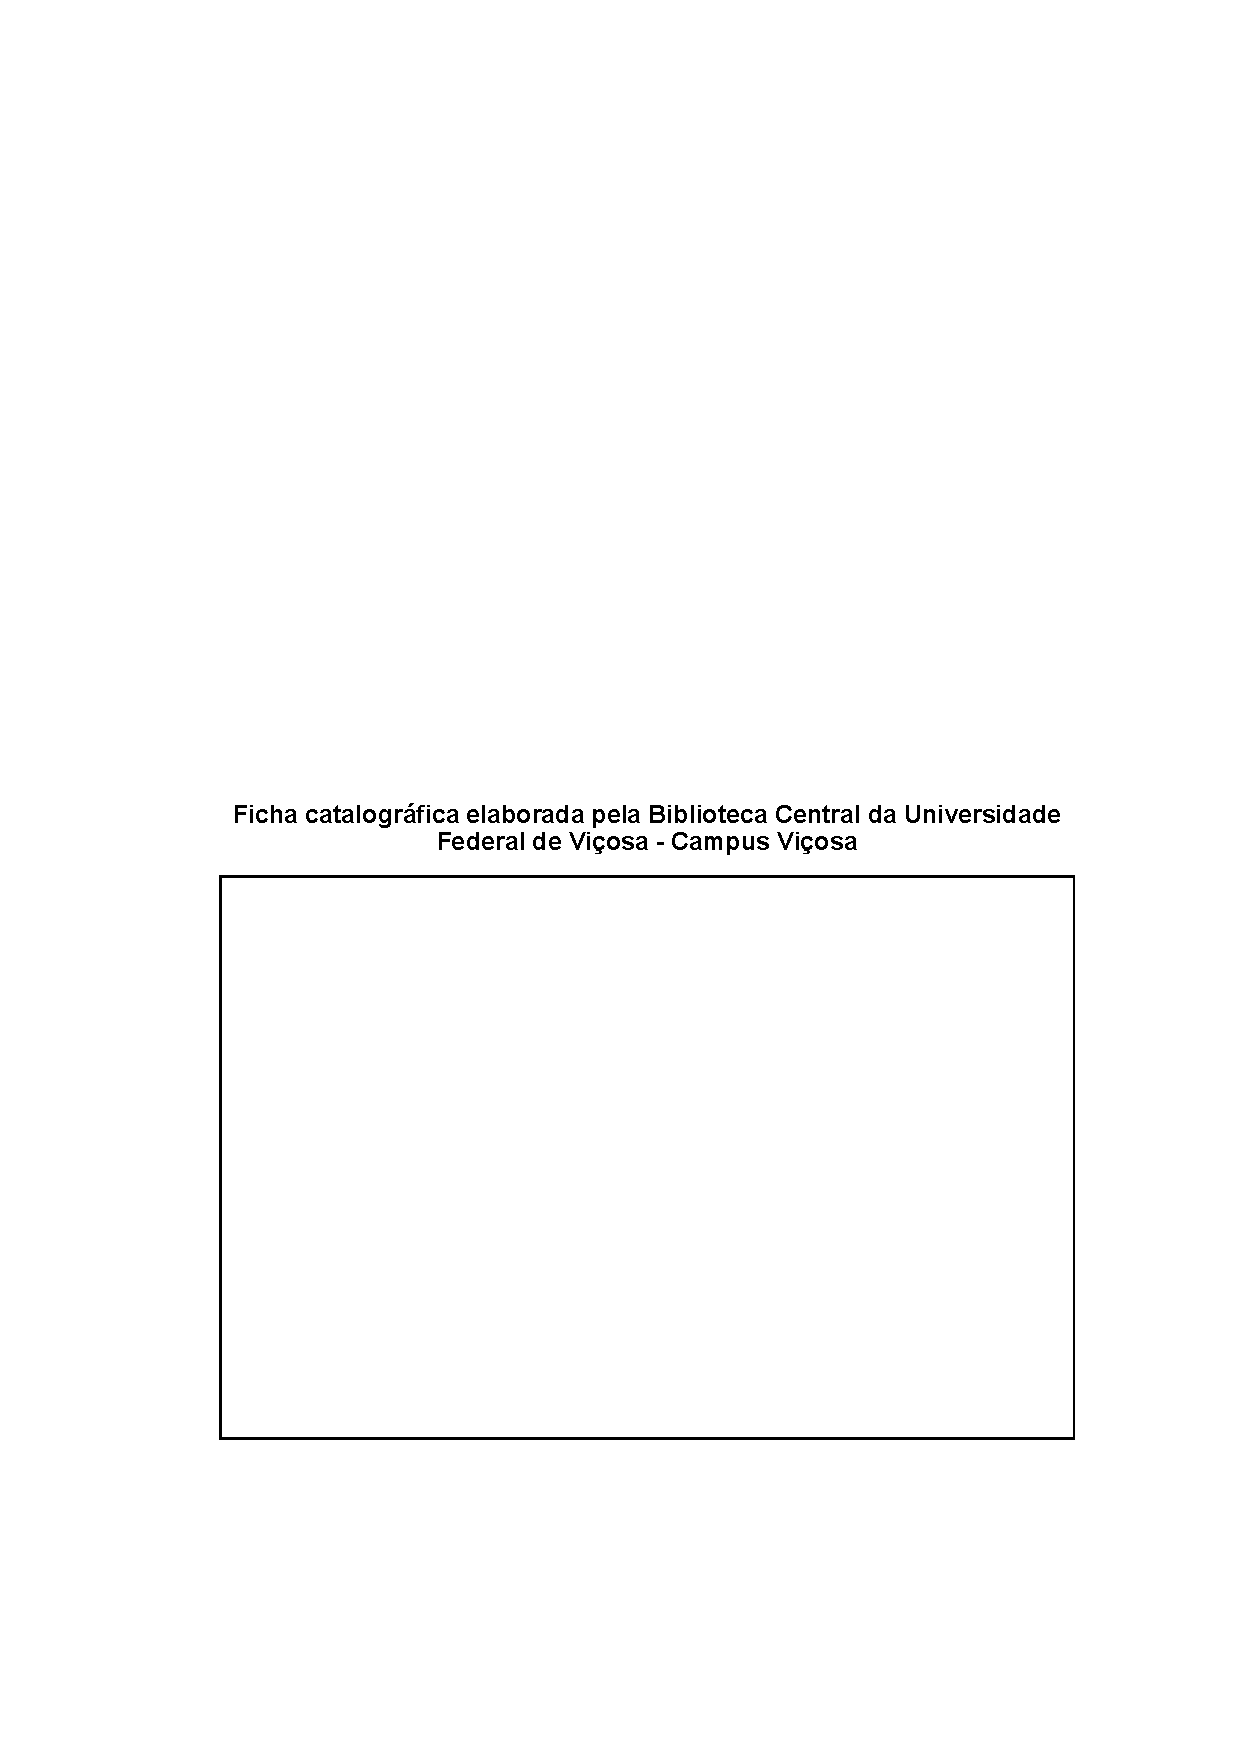
\includepdf[pages=-]{pdfs/ficha-catalografica-branca.pdf}

\imprimirfolhadeaprovacao

\selectlanguage{english}

\huge
\begin{center}
{\fontfamily{lmss}\selectfont Acknowledgements}
\end{center}
%\singlespacing
%\vspace{0.85cm}
\vspace{0.8cm}
\normalsize
%% ACKNOWLEDGEMENTS\\

To the Universidade Federal de Viçosa and the Graduate Program in Computer Science, for the opportunity to pursue my master's degree. I also thank Instituto Brasileiro de Geoegrafia e Estatística (IBGE) for providing the computational infrastructure necessary for the completion of this project.
 
To my advisor, Prof. Dr. Hugo Neves Oliveira, not only for his academic guidance, but also for his friendship, care, and for believing in me even before the start of this project.

To my co-supervisor, Prof. Dr. Jefferson Alex dos Santos, for his valuable contributions, insightful discussions, and critical feedback, which played a crucial role in refining the quality of this research.

To my family, for all their love, example, and dedication, and for teaching me the value of education.

To all my friends - whose list, fortunately, is far too long to mention individually - for listening to me talk about this work for two years without complaint.    
 
And finally, to God, for having created such an incredible and fascinating world to study and learn about.

\cleardoublepage
\cleardoublepage % Garante que comece numa página ímpar (frente)
\thispagestyle{empty} % Remove numeração e cabeçalho desta página

% Empurra o conteúdo para o fundo da página
\vspace*{\fill}

\begin{flushright}
   % A minipage garante que o texto fique contido na metade direita da página
   \begin{minipage}{0.5\textwidth}
      \raggedleft % Alinha o texto à direita dentro da caixa
      \textit{``Suppose we have only dreamed, or made up, all those things-trees and grass and sun and moon and stars and Aslan himself. Suppose we have. Then all I can say is that, in that case, the made-up things seem a good deal more important than the real ones. [...] I’m on Aslan’s side even if there isn’t any Aslan to lead it. I’m going to live as like a Narnian as I can even if there isn’t any Narnia. [...] Not that our lives will be very long, I should think; but that’s a small loss if the world’s as dull a place as you say.''} \\ % Sua frase aqui
      \vspace{0.5cm}
      --- \textsc{Puddleglum - Silver Chair (CS Lewis)} % Nome do autor
   \end{minipage}
\end{flushright}

% Margem inferior opcional para não colar no fim da folha
\vspace*{4cm} 

\cleardoublepage % Garante que a próxima seção comece na página correta

\begin{resumo}[Abstract]
 \begin{otherlanguage*}{english}
   %\noindent


\vspace{\onelineskip}

%\onehalfspacing
\setstretch{1.5}
{
This dissertation proposes and benchmarks a lightweight pipeline for large-scale parcel-level crop classification using time-series data. The key contributions include a scalable SITS download strategy compiled into a open source Python library, a novel parcel-level crop classification dataset construction methodology - including three generated datasets, two for the USA States of Texas and California and a subcontinental dataset encompassing agriculture from Brasil -, a benchmark of supervised classification techniques tested under varied data availability scenarios and a novel anomaly detection methodology \textbf{ORDER} (\textbf{O}open \textbf{R}ecognition for \textbf{D}iscriminative \textbf{E}rror \textbf{R}ebuttal), capable of detecting prediction anomalies of models without requiring retraining. The methodology combines plot design and cropland rasters, basic spectral descriptive statistics extraction from images using cloud computing, state-of-art and consolidated models and SSL pre-training strategies and a reinvention of a classic model for anomaly detection. We benchmarked our pipeline with the three mentioned datasets, builded upon Varda Global FieldID public parcel delineation and USDA NASS Cropland Data and Mapbiomas Brasil public crop class informations. To validate the methodology, we tested the shallow Support Vector Machine, Random Forest, and Multi Layer Perceptron models, the consolidated SITS-BERT and SITS-BERT++ transformer-based models in the literature, and the SITS-CNN (based on the modern ConvNeXt) and SITS-Mamba (based on the Mamba post-transformer model) models adapted by us, with pre-training using Masked Modeling, Momentum Contrast, Fast Siamese, and PMSN. Experimental results show that deep models, such as SITS-BERT++ and a Mamba model proposed by us, outperform Random Forest and Support Vector Machine approaches. The Mamba model, for instance, achieves an Weighted F1 score of 85.0\% in comparison with 77.7\% of a SVM model in the Brazil dataset. We show that SSL pretraining leads to better classification metrics in the finetuned models when compared to random initialization, specially in few-shot cenarios - SITS-BERT++ achieves a near 20\% Weighted F1 Score increase in Brazil when finetuned with only 1\% labeled samples. The ORDER anomaly detection methodology proved promising, generating increased classification metrics in all experiments with deep models, such as a 0.4\% increase in SITS-BERT++ trained from scratch in California dataset, working even when the model classification metrics are already high, a common issue in confidence estimation methods.
}

   \vspace{\onelineskip}

   \noindent
   \textbf{Keywords}: Crop Classification 1. Satellite Image Time Series 2. Anomaly Detection 3. Self-Supervised Learning 4. Open-set Recognition 5.
 \end{otherlanguage*}
\end{resumo}

\cleardoublepage
\pdfbookmark[0]{\listfigurename}{lof}
\listoffigures*
\cleardoublepage

\pdfbookmark[0]{\listtablename}{lot}
\listoftables*
\cleardoublepage

\chapter*{List of abbreviations and acronyms}
\addcontentsline{toc}{chapter}{List of abbreviations and acronyms}

\begin{acronym}[FastSiam] % Usando a mais longa para alinhamento
    \acro{AE}{AutoEncoder}
    \acro{AGDC}{Australian Geoscience Data Cube}
    \acro{ALOS}{Advanced Land Observation Satellites}
    \acro{ASTER}{Advanced Spaceborne Thermal Emission and Reflection Radiometer}
    \acro{BDC}{Brazil Data Cube}
    \acro{BERT}{Bidirectional Encoder Representations from Transformers}
    \acro{BiGRU}{Bidirectional Gated Recurrent Unit}
    \acro{BYOL}{Bootstrap Your Own Latent}
    \acro{CBERS}{China-Brazil Earth-Resources Satellite}
    \acro{CELoss}{Cross-Entropy Loss}
    \acro{CNES}{Centre National d'Études Spatiales}
    \acro{CNN}{Convolutional Neural Network}
    \acro{CV}{Computer Vision}
    \acro{DCAI}{Data Centric Artificial Intelligence}
    \acro{DeCUR}{Decoupling Common and Unique Representations}
    \acro{DINO}{Self-Distillation with No Labels}
    \acro{DL}{Deep Learning}
    \acro{DT}{Decision Tree}
    \acro{DoY}{Day Of the Year}
    \acro{EMR}{Eletromagnetic Radiation}
    \acro{EOS}{Earth Observing System}
    \acro{EO}{Earth Observation}
    \acro{ESA}{European Space Agency}
    \acro{EVI2}{Two-band Enhanced Vegetation Index}
    \acro{EVI}{Enhanced Vegetation Index}
    \acro{FCN}{Fully Convolutional Network}
    \acro{FastSiam}{Fast Siamese}
    \acro{GAN}{Generative Adversarial Network}
    \acro{GB}{Gradient Boosting}
    \acro{GMM}{Gaussian Mixture Model}
    \acro{GEE}{Google Earth Engine}
    \acro{GeMOS}{Generative Models for Open Set}
    \acro{GPT}{Generative Pre-trained Transformer}
    \acro{GPU}{Graphics Processing Unit}
    \acro{GRU}{Gated Recurrent Unit}
    \acro{HR}{High Resolution}
    \acro{HSI}{Hyperspectral Image}
    \acro{IBGE}{Instituto Brasileiro de Geografia e Estatística}
    \acro{INPE}{Instituto Nacional de Pesquisas Espaciais}
    \acro{IoU}{Intersect over Union}
    \acro{IRS}{Indian Remote Sensing}
    \acro{ISRO}{Indian Space Research Organisation}
    \acro{JAXA}{Japan Aerospace Exploration Agency}
    \acro{KNN}{K-Nearest Neighbors}
    \acro{LLM}{Largue Language Model}
    \acro{LR}{Low Resolution}
    \acro{LSTM}{Long Short-Term Memory}
    \acro{LULC}{Land Use and Land Cover}
    \acro{LGBM}{Light Gradient Boosting Machine}
    \acro{LiDAR}{Light Detection and Ranging}
    \acro{mAP}{Mean Average Precision}
    \acro{mAR}{Mean Average Recall}
    \acro{mIoU}{Mean Intersection over Union}
    \acro{MAE}{Masked AutoEncoder}
    \acro{MM}{Masked Image Modeling}
    \acro{MLP}{Multi-Layer Perceptron}
    \acro{ML}{Machine Learning}
    \acro{MODIS}{Moderate Resolution Imaging Spectroradiometer}
    \acro{MR}{Medium Resolution}
    \acro{MoCo}{Momentum Contrast}
    \acro{NASA}{National Aeronautics and Space Administration}
    \acro{NDVI}{Normalized Difference Vegetation Index}
    \acro{NDYI}{Normalized Difference Yellowness Index}
    \acro{NIR}{Near-Infrared}
    \acro{NLP}{Natural Language Processing}
    \acro{OA}{Overall Accuracy}
    \acro{ORDER}{Open-set Recognition for Discriminative Error Rebuttal}
    \acro{OSR}{Open Set Recognition}
    \acro{RF}{Random Forest}
    \acro{RNN}{Recurrent Neural Network}
    \acro{RS}{Remote Sensing}
    \acro{ReLU}{Rectified linear unit}
    \acro{S4L}{Self-Supervised Semi-Supervised Learning}
    \acro{SAM}{Segment Anything Model}
    \acro{SAR}{Synthetic Aperture Radar}
    \acro{SITS}{Satellite Image Time Series}
    \acro{SL}{Shallow Learning}
    \acro{SPOT}{Satellite pour l'Observation de la Terre}
    \acro{SSL}{Self-Supervised Learning}
    \acro{SVM}{Support Vector Machine}
    \acro{SWIR}{Short-Wave Infrared}
    \acro{SeCo}{Seasonal Contrast}
    \acro{SimCLR}{A Simple Framework for Contrastive Learning of Visual Representations}
    \acro{SimMIM}{Simple Masked Image Modeling}
    \acro{SimSiam}{Simple Siamese}
    \acro{SwAV}{Swapping Assignments between Views}
    \acro{UAV}{Unmanned Aerial Vehicle}
    \acro{USDA}{United States Department of Agriculture}
    \acro{USGS}{United States Geological Survey}
    \acro{VHR}{Very High Resolution}
    \acro{VICReg}{Variance-Invariance-Covariance Regularization}
    \acro{VICRegL}{Local Variance-Invariance-Covariance Regularization}
    \acro{VIS}{Visible}
    \acro{VRAM}{Video Random Access Memory}
    \acro{ViT}{Vision Transformer}
    \acro{dB}{Decibel}
\end{acronym}

\pdfbookmark[0]{\contentsname}{toc}
\tableofcontents*
\cleardoublepage

\textual

\chapter{Introduction}\label{chapter:introduction}

\fromsurvey{The \textit{Green Revolution} (1960s and 1970s) \citep{LLEWELLYN2018449} led to a significant increase in agricultural production \citep{evenson2003assessing} through technologies such as pesticides, fungicides, herbicides, and genetically modified crops. This development went hand in hand with the widespread establishment of monocultures and improved machinery for practically all agricultural processes. Local universities and state-owned agencies \citep{franco2001papel} played significant roles in this process. However, this revolution brought some negative aspects, such as technological dependence, deforestation, pollution, and the loss of biodiversity due to the established use of pesticides and monocultures \citep{glaeser2010green}.}

\fromsurvey{Today, as the population continues growing \citep{un_population_2024}, a further leap in agricultural productivity is required \citep{LLEWELLYN2018449}. However, achieving this leap is a greater challenge, as it is essential to mitigate the environmental impact of agribusiness. Moreover, this leap must be implemented in times of current climate problems that are already impacting agricultural productivity \citep{ortiz2021anthropogenic}. Therefore, the dream of sustainable agriculture, that is in harmony with the environment while being more productive, is more important than ever.}

\fromsurvey{In this context, \ac{RS} is a candidate tool to help accomplish this new ``greener revolution'' \citep{ahmed2024examination} as it allows monitoring whether crops are planted and harvested under optimal conditions, the use of precision agriculture \citep{liaghat2010review}, and other innovations such as the avoidance of poor crop rotation practices. For instance, precision agriculture allows agronomists to treat different regions of a field differently, e.g. applying chemicals locally rather than evenly across the plot \citep{zhang2002precision}, resulting in higher productivity while reducing environmental damage. In addition, \ac{RS} allows active monitoring of deforestation and reviewing what use or cover of land has been identified in the deforested area \citep{candra2020deforestation}. \ac{RS} can also predict agricultural productivity in different regions, allowing stakeholders to anticipate food shortages or other crises related to agricultural products \citep{quinn2010increased}.}

\fromsurvey{However, in large-scale crop monitoring, the price of expert data labeling for \ac{RS} can be a drawback \citep{ma2021multi}. The complexity increases with the heterogeneity and size of the \ac{SITS}, which may contain data such as optical, \ac{SAR}, \ac{LiDAR} and as well as thermal imagery, each with different characteristics \citep{joshi2023remote, Brandt2009} making active monitoring in near real-time by human experts infeasible (\autoref{fig:pastis_sits} shows an example of Sentinel 2 SITS labeling). \ac{ML}, especially \ac{DL}, offers a viable solution by enabling the analysis of heterogeneous data \citep{li2022deep} and scaling methods for global, near real-time monitoring. Such techniques have now replaced the traditional Shallow Learning techniques used in the past for Agricultural \ac{RS}, causing a transformation in the literature -- a change best explained through the last correlated survey of the area and the findings found through this review. These techniques can promote sustainable practices, compare patterns between regions with similar conditions, and detect or penalize deforestation, although the price of labeled datasets may still be a limitation.}

\begin{figure}[ht!]
\centering
\caption{Example of a Satellite Image Time Series (SITS) from Sentinel 2 with a labeling process.}
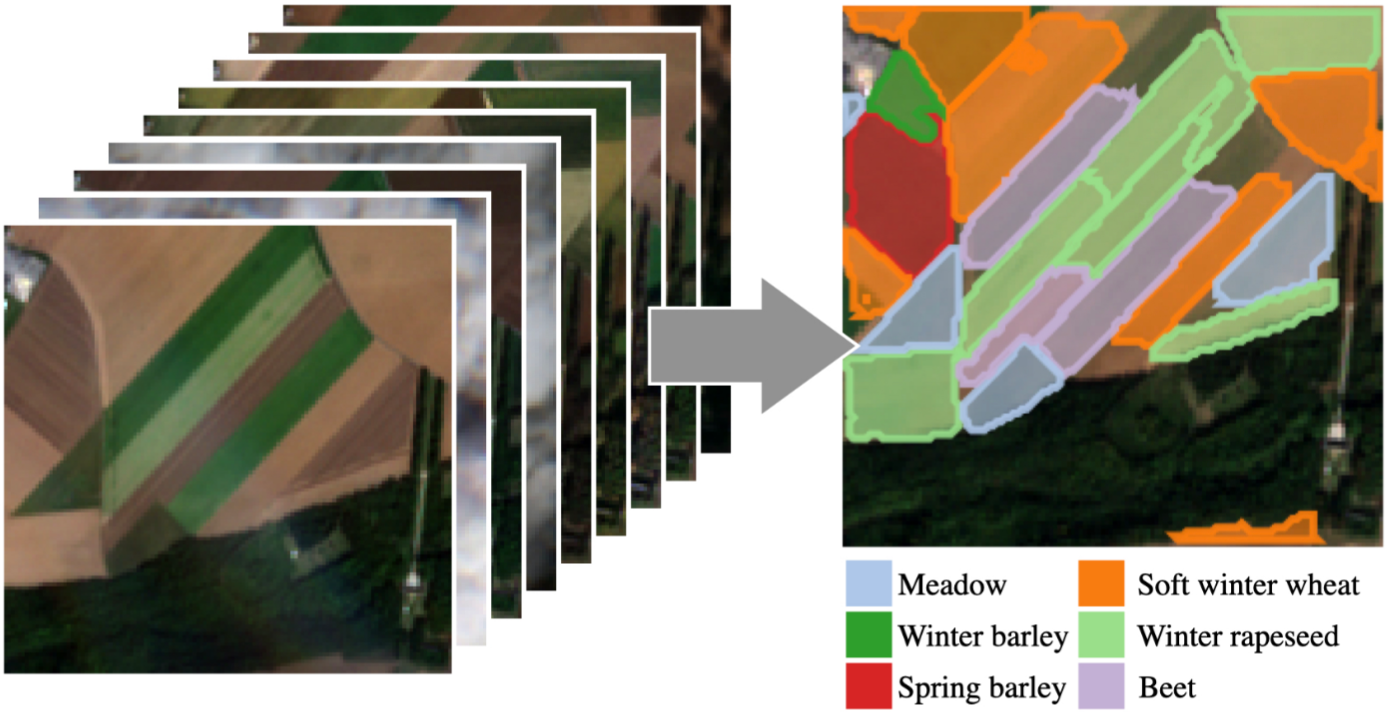
\includegraphics[width=0.75\linewidth]{figures/1_introduction/pastis-sits.png}
\fignote{Adapted from PASTIS dataset \citep{garnot2021panoptic}}
\label{fig:pastis_sits}
\end{figure}

\fromsurvey{It is important to point out that countries such as Brazil, Russia, India and China will play a crucial role in this new green revolution. These regions, in addition to their considerably large area, have significant preserved forests \citep{heino2015forest} and agricultural land \citep{pata2021linking} which makes continuous environmental monitoring essential and positions them as ideal candidates for the application of \ac{RS} techniques. However, due to limited financial resources in some emerging countries, satellite data from public missions becomes essential for supporting environmental applications in these areas.} Furthermore, it is important that the pipelines and models are also lightweight enough to run without the need for expensive hardware, since such countries may not have giant data centers available.

The reliability of predictions is a central challenge in operationalizing machine learning models for agricultural monitoring. The occurrence of incorrect classifications, or false positives generated by samples outside the training distribution, can severely compromise production estimates and the efficiency of resource allocation. It is possible that \ac{OSR} techniques such as \ac{GeMOS} \citep{vendramini2021opening} can, in addition to identifying class samples outside the training set, also possibly differentiate correct from incorrect predictions within known classes.

\fromsurvey{Moreover, the amount of unlabeled remote sensing data is considerable, as satellite images are constantly being acquired by various free-of-charge missions. This is one of the reasons why \ac{SSL} is very promising in the field of \ac{RS}, as it is able to extract patterns from unlabeled data to generate supervised signals by reconstructing masked data or data contrastivity. \ac{SSL} has became very popular in \ac{NLP} and is one of the reasons for the success of tools such as \ac{GPT} \citep{radford2018improving} and large language models such as \ac{BERT} \citep{devlin2019bert}. Thus, after pretraining a \ac{DL} model with \ac{SSL}, it is possible to train it with less labeled data, resulting in a model that is likely to be more robust and generalistic \citep{chen2020adversarial}.}

\fromsurvey{Thus, we comprehensively reviewed all publicly available labeled datasets for these applications, focusing on both agricultural and deforestation classes, including the few datasets whose study regions are emerging countries. In addition, we reviewed all satellite sensors that are publicly available to researchers and/or contain some publicly available datasets that could be useful for the research area. We also included unlabeled \ac{RS} datasets, as we have not yet found any unlabeled datasets specifically for \ac{RS} of agriculture or vegetation.}

Furthermore, it is clear that for large-scale crop monitoring, the use of paid remote sensing images becomes impractical. It is possible to imagine a pipeline divided into three main sequential stages:

\begin{enumerate}
    \item \textbf{Parcel Delineation} Identifying the geometries of agricultural plots on a given farm or in any given region.
    \item \textbf{Crop Mapping} Given the geometry of an agricultural plot, classify the species of plant grown in a given period of time.,
    \item \textbf{Crop Yielding} Given the geometry and the species of plant grown, predict what the yield (usually in tons per hectare) of that crop will be.
\end{enumerate}

In addition, there are two other applications that are more peripheral to crop monitoring, but equally important: Change Detection and Land Usage Land Cover. The first can be used to detect deforestation, which may be a step prior to planting a crop. The second can be used for more general mapping of a farm in order to detect the amount of water, for example, which can be used to refine a crop classification, since certain species require active irrigation.  

\begin{figure}[!ht]
  \caption{Diagram showing possible agricultural (a) and correlated (b) applications with Deep Learning and Remote Sensing.}
  \centering
  \begin{subfigure}[c]{0.48\columnwidth} % Reduced width
    \centering
    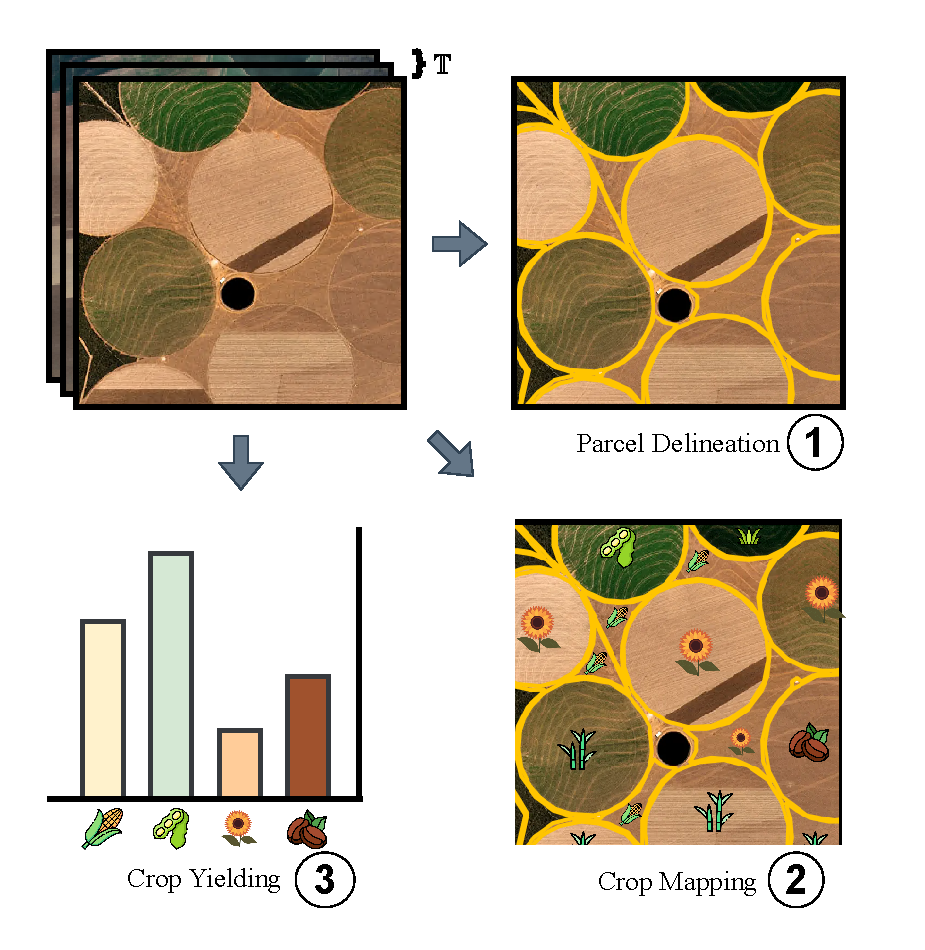
\includegraphics[width=\currprop]{figures/1_introduction/graphical_abstract_crop_new_fixed.pdf} % + 0.19
    \caption{}
    \label{fig:graphical_abstract_crop_tasks}
  \end{subfigure}
  \hfil % This provides the horizontal space
  \begin{subfigure}[c]{0.48\columnwidth} % Reduced width
    \centering
    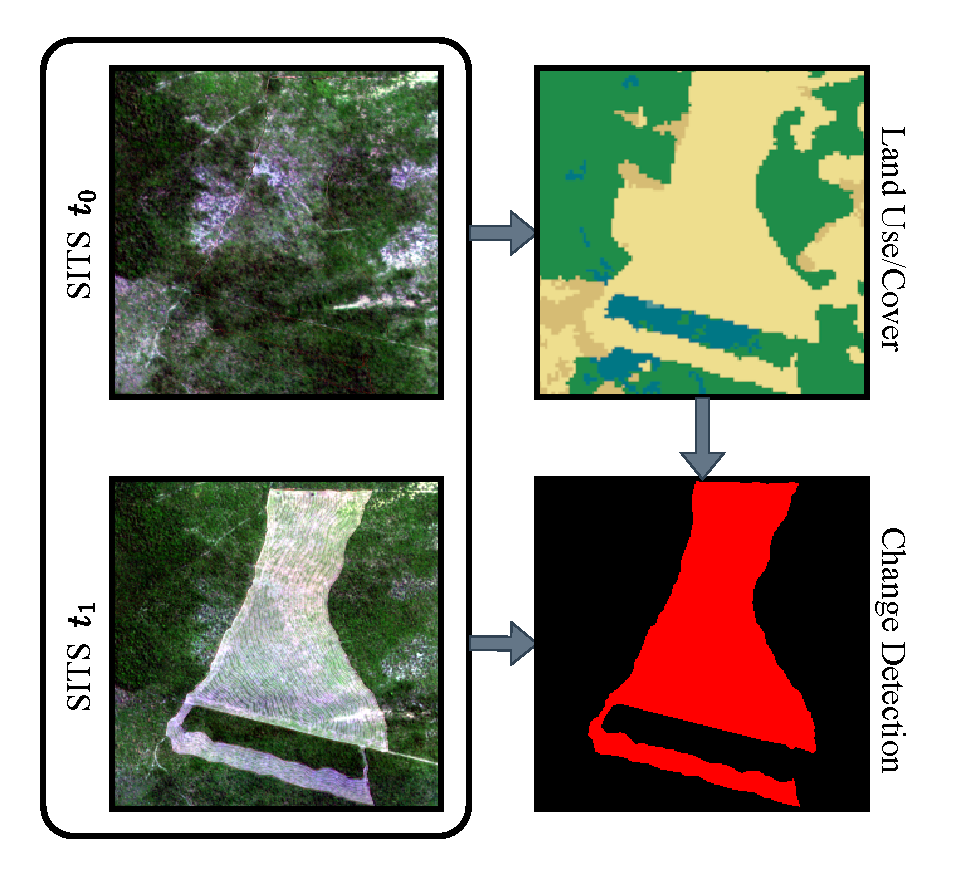
\includegraphics[clip,width=\currprop]{figures/1_introduction/graphical_abstract_lulc_cd_new.pdf}
    \caption{}
    \label{fig:graphical_abstract_lulc_cd}
  \end{subfigure}
  
  \fignote{This figure shows illustrative examples of the applications covered in this work. In Figure \ref{fig:graphical_abstract_crop_tasks}, we can observe a large-scale crop monitoring pipeline based on (1) parcel delineation, (2) crop mapping and (3) crop yielding prediction illustrated over multitemporal images. In Figure \ref{fig:graphical_abstract_lulc_cd}, two timestamps are used to compute land cover/usage and change detection. Most agricultural-related applications rely on multitemporal data across a range $\mathbb{T}$ of acquisition dates (a) or a pair $t_0$ and $t_1$ of dates (b).}
  
  \label{fig:graphical_abstract}
\end{figure}

In this study, we focus specifically on Crop Mapping, since Parcel Delineation already has foundational models that allow the application to be run without training data (see Section \ref{sec:parcel_segmentation}) and Crop Yielding has very few public datasets (see Section \ref{sec:labeled_datasets}) due to the industry's economic interest in the area, meaning that most datasets are private and focus on a subset of crop classes relevant to a geographic region. We propose a complete pipeline ranging from a rigorous strategy for building a crop mapping dataset from parcel geometries and public cropland rasters, a lightweight method for downloading samples from public mission sensors, evaluation of Shallow Learning and Deep Learning models for classification, SSL pre-training techniques, and procedures for anomaly detection.

Regarding the work developed throughout the master's program, a literature review was published at an international conference \citep{mateuzin2024} awarded with an extended version published in Computer \& Graphics \citep{daSilva2025} with a new culture classification model proposed using \ac{SSL}. In addition, part of the methodology of this dissertation work was also published as a separate paper \citep{pintodasilva2025lightweight}. Two co-supervisions of bachelor's degree final projects were conducted, one in the area of Open Set Recognition for Crop Classification and the other for super-resolution for agricultural Remote Sensing. Finally, three less related works were done, one as a result of teaching assistance in a programming course using \ac{LLM} \citep{alcantara2025assessing}, another for segmentation of 3D medical images \citep{Oliveira2025} and another about the role of data quality in remote sensing classification \citep{Correa2026rethinking}. At last, a Python library with tools for downloading and preprocessing data that can be fed to the pipeline was also published on PyPI (more details in Section \ref{sec:agl}).

\section{Research Questions}

To guide the investigation into the gaps identified in large-scale agricultural monitoring – scarcity of reliable labeled data, possible hardware limitations, use of only publicly available sensor data due to the high price of paid sensor data, and verification of correct/incorrect predictions with anomaly detection – this work is structured around six fundamental Research Questions (RQs).

\begin{enumerate}
    \item \textbf{RQ1:} To what extent can DCAI strategies - specifically, rigorous filtering of noisy public labels (such as USDA CDL or Mapbiomas) - enable the creation of crop classification datasets and improve the performance of crop classification models?
    \item \textbf{RQ2:} Do SSL pre-training strategies impact embedding generation and offer a significant advantage over supervised models when labels are scarce? If so, which strategy generates the best embeddings?
    \item \textbf{RQ3:} Is it possible to build a lightweight pipeline that achieves satisfactory performance for crop classification that can be run without expensive hardware? If so, which models are most suitable?
    \item \textbf{RQ4:} Is it possible to achieve satisfactory performance for crop classification using only public sensors?
    \item \textbf{RQ5:} Is it possible to improve confidence estimation or detect model anomalies - differ between right and wrong predictions - through generative models on embeddings, surpassing established baselines such as ConfidNet \citep{corbiere2019addressing} in the task of fault prediction?
\end{enumerate}

\section{Aims and Objectives}

The main objective of this work is to develop and validate a reliable, lightweight, data-centric pipeline for crop classification at the plot level, using public SITS, capable of distinguishing between known and unknown crops and predicting its own failures. The specific objectives are:

\begin{itemize}
    \item Analyze and curate publicly labeled agricultural datasets from large producers (US and Brazil), applying data-centric filtering techniques to mitigate label noise;
    \item Evaluate the suitability of public sensors (Sentinel-2) for capturing spectral-temporal patterns of crops.
    \item Implement and publicize a lightweight pipeline for downloading and preprocessing SITS time series of optical data from parcel geometries;
    \item Implement and compare DL/SL architectures in terms of metrics and computational cost.
    \item Investigate the impact of different SSL pre-training techniques on the quality of the generated embeddings and their transfer learning capability;
    \item Develop and validate a DCAI confidence estimation strategy based on generative model optimization (called \ac{ORDER}, based on \ac{GeMOS} \citep{vendramini2021opening}) and compare it with the ConfidNet \citep{corbiere2019addressing} baseline to detect incorrect predictions.
\end{itemize}

\section{Contributions}

To achieve the aforementioned objectives and address the research questions posed in this study, this thesis proposes a comprehensive methodology that spans from rigorous data curation and lightweight data acquisition to extensive model benchmarking and advanced anomaly detection. Specifically, the main contributions of this work to the fields of Agricultural Remote Sensing and Machine Learning are summarized as follows:

\begin{itemize}
    \item \textbf{Curation Methodology for creating parcel-level crop classification datasets:} We propose a rigorous protocol for filtering and cleaning noisy public labels based on a Cropland raster and parcel delineation, which generates a parcel-level crop classification dataset to train the models in the subsequent steps;
    \item \textbf{Lightweight SITS Download Methodology:} We develop an efficient method for downloading satellite image time series (SITS) using Google Earth Engine (GEE), optimizing the process to reduce computational costs and download time;
    \item \textbf{Evaluation of Simple vs. Complex Models:} Comparative analysis showing the effectiveness of lightweight architectures (MLPs and SL) compared to DL models, ranging from 1D CNN, LSTM, Transformer to the post-transformer MAMBA architecture;
    \item \textbf{SSL Pre-training Benchmark}: Comparative evaluation of reconstruction (MIM), contrastive (MoCo), non-contrastive (FastSiam), and hybrid (PMSN) strategies for pre-training models in agricultural SITS.
    \item \textbf{Development of the \ac{ORDER} Method:} We propose \ac{ORDER}, a hyperparameter search strategy applied to the \ac{GeMOS} \cite{vendramini2021opening} framework. Unlike standard anomaly detection, \ac{ORDER} maximizes the Area Under the Curve (AUC) by specifically considering the separability between correctly and incorrectly classified samples for each class;
    \item \textbf{Confidence Estimation Benchmarking:} We perform a comparative evaluation of model reliability using ConfidNet \citep{corbiere2019addressing} as a baseline against the proposed \ac{ORDER} approach, focusing on maximizing failure prediction;
    \item \textbf{Open Source Tools:} Publication of the time series download method, among other additions, in the AgriGEE.lite library to facilitate research in the area.
\end{itemize}

\section{Thesis Outline}

The remainder of this thesis is organized as follows. Chapter \ref{chapter:theoretical_background} introduces the necessary theoretical background, addressing concepts of Agricultural Remote Sensing, observation satellites, and Machine Learning principles, from \ac{SL} to \ac{DL}, also detailing \ac{SSL}. Next, Chapter \ref{chapter:related_works} presents a review of related works and a taxonomy of the area, covering applications directly related to agriculture -- Parcel Delineation, Crop Mapping, and Crop Yielding -- and indirect applications -- \ac{LULC} and Change Detection.

The Chapter \ref{chapter:meth_data} describes data acquisition and datasets made from \ac{SITS}, detailing the pipeline for creating parcel-level datasets for the regions of Texas, California, and Brazil, as well as the lightweight download strategy implemented in the AgriGEE.lite library. Subsequently, Chapter \ref{chapter:meth_model} explores the learning methods used in the study, including \ac{SL}, \ac{DL}, and \ac{SSL}, as well as techniques aimed at anomaly detection.

The experimental setup is defined in Chapter \ref{chapter:exp_setup}, which lists the evaluation metrics employed, hardware used, hyperparameter search space, tests performed, and data scenarios considered. Finally, Chapter \ref{chapter:results} reports the quantitative results obtained, both from pre-training and generated embeddings, as well as from fine-tuning. It also discusses the findings in the context of the current literature and technological changes in the field. At last, Chapter \ref{chapter:conclusion} presents the concluding remarks of this work, summarizing the contributions and answering the research questions.
\chapter{Theoretical Background}\label{chapter:theoretical_background}

This chapter establishes the theoretical foundations that underpin this research, organized into four sections, serving as a leveling ground for the reader. In the \autoref{sec:ag_contextualization} section, essential concepts of agricultural \ac{RS} are presented, including a review of vegetation indices, Earth observation satellites, and a review of public datasets available in the literature. Next, in the \autoref{sec:ml_contextualization} section, the principles of \ac{ML} are discussed, ranging from classic \ac{SL} models to state-of-the-art \ac{DL} architectures, such as Transformers and post-Transformer architectures. The \autoref{sec:ssl_contextualization} explores \ac{SSL}, detailing contrastive, masked modeling, and hybrid techniques widely used to train some of the latest models. Finally, the \autoref{sec:conf_contextualization} section describes the problem of confidence detection in predictions, including anomaly detection.


\section{Agricultural Remote Sensing}
\label{sec:ag_contextualization}

\fromsurvey{\ac{RS} can be defined as the field that studies, from a distance, objects and phenomena \citep{Jensen2014}. Remotely sensed data can be acquired from non-contact sensor systems, such as satellites, planes, and drones. All sensors are based on the study of \ac{EMR} and the ability of individual targets to reflect, absorb, and transmit this \ac{EMR} \citep{Jensen2014, Brandt2009}. According to the authors, there are two main types of sensors: (i) passive and (ii) active. Passive sensors are those that can only receive \ac{EMR}, such as optical and thermal sensors. Active sensors are those that can transmit and receive \ac{EMR}, such as \ac{SAR} and \ac{LiDAR}\footnote{Please refer to Jensen \citep{Jensen2014}.}.}

\fromdatacentricai{Except for \ac{LiDAR} data, remote sensing images are usually stored as raster files, usually in TIFF \citep{poynton1992overview} or NetCDF \citep{rew1990netcdf} formats. The term ``raster'' originally comes from the Latin rastrum, meaning ``rake,'' referring to something that ``sweeps'' a surface. In the context of computer graphics and geotechnology, it has been adopted to describe how digital images are organized in a matrix structure \citep{jensen2015introductory, novo2013sensoriamento}. The adoption of the term is also related to the process of acquiring remote sensing images, which often occurs through line-by-line scanning, similar to a systematic sweeping of the terrain.}

\fromsurvey{\ac{LiDAR} and \ac{SAR} sensors are known to be very useful for remotely sensed data. The former is filling an enormous gap in remotely sensed data: more accurate height variations, i.e. 3D data \citep{wangChallengesOpportunitiesLidar2021}. These 3D data can be used to estimate crops and canopy height, which, in its turn, is used for biomass estimation \citep{riveraLiDARApplicationsPrecision2023}. As for the latter, \ac{SAR}, \cite{liuResearchAdvancesSAR2019} explain that \ac{SAR} \ac{EMR} can penetrate clouds, which enables crop monitoring throughout the year without interference. The authors also stated that \ac{SAR} has been quite useful for crop identification because its backscatter is affected by biomass structure, solid condition and provides improved accuracy when used with different polarizations.}

\fromsurvey{Even though \ac{SAR} and \ac{LiDAR} sensors are extremely useful for remote sensing, they are not yet widely used due to their revisit time, which is lower than optical satellite data \citep{Jensen2014}}, This limitation has been further exacerbated by the reported malfunction of one of the most widely used \ac{SAR} sensors, Sentinel-1B, which became inoperative on December 23, 2021 \footnote{Mission ends for Copernicus Sentinel-1B satellite - \url{https://www.esa.int/Applications/Observing_the_Earth/Copernicus/Sentinel-1/Mission_ends_for_Copernicus_Sentinel-1B_satellite}}, resulting in a significant data gap, particularly in some regions (see Table \ref{tab:context-satellites}). \fromsurvey{Another drawback is that their process is far more complex than optical data. \ac{SAR} data needs to be chosen according to the necessity: the polarization, ascending or descending orbit, single look complex, etc. This data is also provided in \ac{dB}, a logarithmic scale. Besides, \ac{SAR} usually follows the Rayleigh distribution \citep{kuruogluModelingSARImages2004}, unlike most optical data that follow the normal distribution. This indicates preprocessing for \ac{SAR} data, which requires computational effort and specific knowledge for processing it. As for \ac{LiDAR} data, it is a point cloud that needs to be processed into a model to be later used as an input for machine learning models  \citep{riveraLiDARApplicationsPrecision2023}. In a nutshell, both \ac{SAR} and \ac{LiDAR} data are not as easy to process and explain as optical data is.}

\fromsurvey{When it comes to optical sensors, we can study how each target can respond to each size of electromagnetic wave, which usually vary from \ac{VIS} - from 450 to 750 nm - to \ac{NIR} - from 750 to 1300 nm - by its reflectance value. Based on that, researchers could describe the spectral behavior for each target, in a sense that the analyst can distinguish types of land cover (eg. water, vegetation, bare soil) and understand its characteristics \citep{plants12122347}. From these different spectral responses, it is even possible to differentiate crops, as shown in Figure \ref{fig:context_reflectances1}. This Figure presents different patterns for each type of crop (corn, sugarcane, coffee, canola, wheat, tobacco) according to their respective factor of reflectance.}

\fromsurvey{For a thorough observation in Figure \ref{fig:context_reflectances1}, wheat is more easily distinguished from the other crops, once its reflectance is higher for almost all wavelengths, mainly \ac{NIR} and \ac{SWIR}. On the other hand, tobacco can be distinguished better at \ac{VIS}, in wavelengths close to yellow and so forth.}

\begin{figure}[!ht]
    \centering
    \caption{\fromsurvey{Example of spectral behavior of different crops classes.}}
    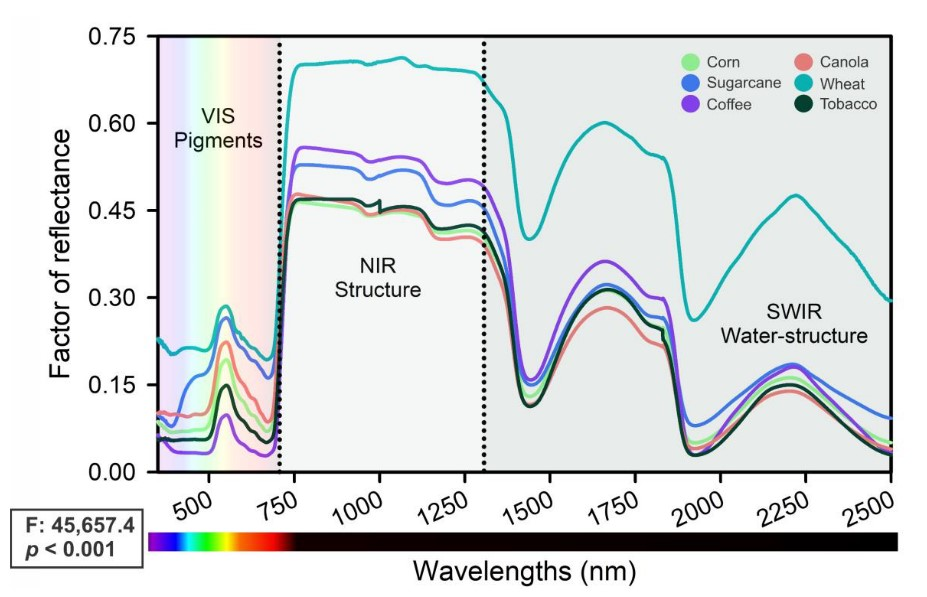
\includegraphics[width=0.95\linewidth]{figures/3_theoretical_background/veg_reflectance.jpg}
    \fignote{ The wavelengths refer to: visible (VIS), near-infrared (NIR) and short-wave infrared (SWIR). Adapted from \cite{plants12122347}}
    \label{fig:context_reflectances1}
\end{figure}

\subsection{Vegetation Indices}

\fromsurvey{From the spectral reflectance, researchers studied methods for better understanding targets and how to discriminate them. They created vegetation indices that, for agriculture, can help analysts to describe vegetation health and age. These indices aim to highlight part of the image with different vegetation cover; they are usually obtained by dividing two spectral bands with high and low reflectance values, respectively \citep{bannari1995review,gao2020remote, ReflectanciaDosMateriais2021}. They are related to spectral estimates for biochemical and biophysical analyses, such as the chlorophyll content and biomass \citep{ndvi1}. Wavelengths approximately between 700 nm up to 1400 nm (\ac{NIR} and \ac{SWIR}) reflect better vegetation than other land covers, such as dry soil and water, while red wavelengths ($\approx$ 660 nm) do not \citep{Jensen2014}.}

\fromsurvey{Some of the most used indices are \ac{NDVI} \citep{ndvi1}, \ac{EVI} \citep{evi1}, \ac{EVI2} \citep{evi2} and \ac{NDYI} \citep{ndyi1} As previously mentioned, all of them consider bands with high reflectance and low reflectance, respectively. \ac{NDVI} was one of the first indices used in \ac{RS}, using red reflectance values ($\rho_{red}$) and \ac{NIR} ($\rho_{NIR}$); it is presented in Equation \ref{eq:ndvi}. This index is extensively used for agriculture, and it has proven to indicate start of seasons and concern for field assessments \citep{FAOfoodandagricultureorganizationoftheunitednationsGuidelinesUseRemote2018}. On the other hand, \ac{EVI} uses the blue reflectance  ($\rho_{blue}$) together with aerosol resistance ($C_1$ and $C_2$) and canopy background ($L$); it is adjusted not to saturate in high-density canopy cover (Equation \ref{eq:evi}). \ac{EVI2} adjusted \ac{EVI} to only two bands, and the authors state that there is no statistical difference between them. As can be seen, if $L=0$, then \ac{EVI2} is very similar to \ac{NDVI}. \ac{EVI} and \ac{EVI2} are used. In general, \ac{NDVI} usually highlights crop flourishing and indicates the amount of humidity in the parcel. On the other hand, \ac{NDYI}, \ac{EVI} and \ac{EVI2} are used to highlight and understand vegetation peaks of crops and differentiate dense structures.}


\begin{equation}
\label{eq:ndvi}
    NDVI = \frac{\rho_{NIR} - \rho_{red}}{\rho_{NIR} + \rho_{red}}
\end{equation}

\begin{equation}
\label{eq:evi}
        EVI = 2.5 \frac{\rho_{NIR} - \rho_{red}} {L + \rho_{NIR} + C_1\rho_{red}-C_2\rho_{blue}}
\end{equation}

\begin{equation}
\label{eq:evi2}
    EVI2 = 2.5 \frac{\rho_{NIR} - \rho_{red}}{\rho_{NIR} + \rho_{red} + L}
\end{equation}

\begin{equation}
\label{eq:ndyi}
    NDYI = \frac{\rho_{green} - \rho_{blue}}{\rho_{green} + \rho_{blue}}
\end{equation}

\subsection{Earth Observation Satellites}
\label{sec:context_satellites}

\fromsurvey{Since the 1970s, earth observation satellites have been developed to monitor target tasks with specific spectral responses, including vegetation, soil, water, and climate variables. The United States' \ac{NASA} initiated the Landsat program in 1972, creating the longest continuous global land observation record \citep{masek2020,wulder2022}, while its \ac{EOS} expanded capabilities with sensors like \ac{MODIS} and \ac{ASTER} \citep{nasa2020}. The \ac{ESA} developed the Copernicus program with its Sentinel satellite series (2014-present) for open global monitoring \citep{esa2021}, building on earlier ERS and Envisat missions \citep{attema2007}. China's CNSA (China National Space Administration) deployed the Gaofen series (2013-present) and collaborated with Brazil's \ac{INPE} on the \ac{CBERS} program (since 1999) \citep{li2022,lino2000cbers}, with Brazil later launching its first independent satellite Amazonia-1 in 2021 \citep{amazonia2021}. France's \ac{CNES} pioneered commercial high-resolution imaging through \ac{SPOT} (1986-2012) and Pleiades (2011-present) satellites \citep{spot2012,gleyzes2012pleiades}, while India's \ac{ISRO} established regional monitoring via its \ac{IRS} program (1988-present) \citep{navalgund2007}. Also, \ac{JAXA} has missions such as the \ac{ALOS}, a program started in 2006, aiming to provide data for environmental and resource sciences.}


\fromsurvey{
Most EO optical satellites feature specific spectral bands, called \textbf{spectral resolution} \citep{jensen2016}, for different wavelengths:
\begin{itemize}
    \item \textbf{Blue} ($\approx 450-520$ nm),
    \item \textbf{Green} ($\approx 520-600$ nm),
    \item \textbf{Red} ($\approx 630-690$ nm),
    \item \textbf{Near-infrared} (NIR, $\approx 760-1300$ nm),
    \item \textbf{Shortwave infrared} (SWIR, $\approx 1550-1750$ nm and $\approx 2080-2350$ nm).
\end{itemize}}

\fromsurvey{Another crucial aspect of all kinds of remote sensing data is the \textbf{spatial resolution} (the length of one pixel side), classified as:
\begin{itemize}
    \item \textbf{\Acf{VHR}}: $\leq$ 2 m (e.g., WorldView-4),
    \item \textbf{\Acf{HR}}: 2-10 m (e.g., Sentinel-2),
        \item \textbf{\Acf{MR}}: 10-100 m (e.g., Landsat-9),
        \item \textbf{\Acf{LR}}: $\geq$ 100 m (e.g., MODIS) \citep{belward2015}.
\end{itemize}}

\fromsurvey{Also, a critical parameter is the imaging frequency for a given area \citep{wulder2019}, called \textbf{temporal resolution} or \textbf{revisit time}.}

\fromsurvey{The Earth observation data ecosystem includes significant contributions from private companies such as Planet, Maxar, and Airbus, which operate constellations from low up to high-resolution satellites \citep{planet2023,maxar2022,airbus2021}. While these commercial systems provide valuable capabilities for specific applications, our study focuses exclusively on publicly available datasets from programs like Landsat  - \ac{NASA}/\ac{USGS} -  and Sentinel (\ac{ESA}), which offer long-term, research-friendly, open data policies essential for scientific research and global environmental monitoring \citep{masek2020,esa2021}. This emphasis on open data ensures reproducibility and equitable access to Earth observation information across the scientific community. In this direction, some recent initiatives like the \ac{BDC} and \ac{AGDC} simplified \ac{EO} data access by providing easy-to-consume, analysis-ready multitemporal and multisensor data cubes \citep{camara2020,giuliani2020earth}.}

\fromsurvey{Table \ref{tab:context-satellites} summarizes the main satellites referenced in this review, with consolidated information from the \textbf{eoPortal}\footnote{\url{https://www.eoportal.org/}} catalog \citep{eoportal2023}.}


\begin{table}[!ht]
\centering
\caption{\fromsurvey{Main satellite missions used by the selected datasets.}}
\label{tab:context-satellites}

\resizebox{\textwidth}{!}{
\begin{tabular}{lllllllllll}
\hline
\textbf{Mission} && \textbf{Launch} && \textbf{Sensor}&& \textbf{\begin{tabular}[c]{@{}l@{}}Spatial\\ Resolution\end{tabular}} && \textbf{\begin{tabular}[c]{@{}l@{}}Spectral\\ Resolution\end{tabular}}&& \textbf{\begin{tabular}[c]{@{}l@{}}Revisit\\ (days)\end{tabular}} \\ \hline
Landsat-1 (L1)*&& 1972&& MSS&& $\sim$80 m&& VIS, NIR&& 18\\ \hline
Landsat-2 (L2)*&& 1975&& MSS&& $\sim$80 m&& VIS, NIR&& 18\\ \hline
Landsat-3 (L3)*&& 1978&& RBV&& \begin{tabular}[c]{@{}l@{}}$\sim$40 m,\\ $\sim$80 m\end{tabular}&& PAN, VIS, NIR && 18\\ \hline
Landsat-4 (L4)*&& 1982&& TM && $\sim$30 m&& \begin{tabular}[c]{@{}l@{}}VIS, NIR,\\ SWIR, Thermal\end{tabular} && 16\\ \hline
Landsat-5 (L5)*&& 1984&& TM && $\sim$30 m&& \begin{tabular}[c]{@{}l@{}}VIS, NIR,\\ SWIR, Thermal\end{tabular} && 16\\ \hline
SPOT && 1986&& \begin{tabular}[c]{@{}l@{}}HRV, HRVIR,\\ Vegetation\end{tabular} && 1.5-20 m&& VIS, NIR&& 2-3 \\ \hline
POES, MetOp&& 1998&& AVHRR&& $\sim$1.1 km&& VIS, NIR, Thermal && 0.5 \\ \hline
Landsat-7 (L7) && 1999&& ETM+ && $\sim$30 m&& \begin{tabular}[c]{@{}l@{}}VIS, NIR,\\ SWIR, Thermal\end{tabular} && 16\\ \hline
MODIS&& 1999&& Terra, Aqua&& \begin{tabular}[c]{@{}l@{}}250 m, 500 m\\ 1 km\end{tabular} && \begin{tabular}[c]{@{}l@{}}VIS, NIR,\\ SWIR, Thermal\end{tabular} && 1-2 \\ \hline
QuickBird-2&& 2001&& Pan, Ms&& \begin{tabular}[c]{@{}l@{}}0.61 m,\\ 2.44 m\end{tabular}&& VIS, NIR&& 3-7 \\ \hline
ALOS && 2006 &&  \begin{tabular}[c]{@{}l@{}}PALSAR (L-band)\\ AVNIR-2 \\ PRISM\end{tabular} && \begin{tabular}[c]{@{}l@{}}7-44 m\\ 10 m \\ 2.5 m\end{tabular} &&  \begin{tabular}[c]{@{}l@{}}HH+HV or VV+VH\\ RGB-NIR \\ PAN\end{tabular} && 46\\ \hline 
GeoEye-1 && 2008&& MS, PAN&& \begin{tabular}[c]{@{}l@{}}0.41 m,\\ 1.65 m\end{tabular}&& VIS, NIR&& 3-5 \\ \hline
WorldView-2(WV2) && 2009&& Pan, Ms&& \begin{tabular}[c]{@{}l@{}}0.46 m,\\ 1.84 m\end{tabular}&& VIS, NIR&& 1.1 \\ \hline
\begin{tabular}[c]{@{}l@{}}Suomi-NPP,\\ NOAA-20\end{tabular} && 2011&& VIIRS&& 375 m && \begin{tabular}[c]{@{}l@{}}VIS, NIR,\\ SWIR, Thermal\end{tabular} && 1 \\ \hline
Landsat-8 (L8) && 2013&& OLI, TIRS&& $\sim$30 m&& \begin{tabular}[c]{@{}l@{}}VIS, NIR, SWIR,\\ Thermal, Cirrus\end{tabular} && 16\\ \hline
Planet && 2013&& PlanetScope&& 3-5 m && VIS, NIR&& 1 \\ \hline
Sentinel-1 (S1)&& 2014&& SAR C-Band && 10 m&& VV, VH, HV&& 12\\ \hline
CBERS-4&& 2014&& \begin{tabular}[c]{@{}l@{}}PAN, MUX,\\ WFI\end{tabular}&& 5-20 m&& VIS, NIR&& 26\\ \hline
GaoFen-2 (GF2)** && 2014&& PAN, MS&& \begin{tabular}[c]{@{}l@{}}1 m,\\ 4 m\end{tabular}&& VIS, NIR&& 5 \\ \hline
WorldView-3 (WV3)&& 2014&& \begin{tabular}[c]{@{}l@{}}Pan, MS,\\ SWIR\end{tabular}&& \begin{tabular}[c]{@{}l@{}}0.31 m,\\ 1.24 m,3.7 m\end{tabular}&& VIS, NIR, SWIR&& 1 \\ \hline
ALOS-2 && 2014 && PALSAR-2 (L-Band) && 10 m && HH+HV or VV+VH && 16\\ \hline
Sentinel-2 (S2)&& 2015&& MSI&& 10-60 m && \begin{tabular}[c]{@{}l@{}}VIS, NIR,\\ SWIR, RedEdge\end{tabular} && 5 \\ \hline
Sentinel-3 (S3)&& 2016&& \begin{tabular}[c]{@{}l@{}}SLSTR,\\ OLCI, SRAL\end{tabular}&& \begin{tabular}[c]{@{}l@{}}300 m,\\ 1 km\end{tabular} && \begin{tabular}[c]{@{}l@{}}VIS, NIR,\\ SWIR, Thermal\end{tabular} && 1-2 \\ \hline
CBERS-4A && 2019&& PAN, MUX && 5-10 m&& PAN, VIS, NIR && 31\\ \hline
Landsat-9 (L9) && 2021&& \begin{tabular}[c]{@{}l@{}}OLI-2,\\ TIRS-2\end{tabular}&& $\sim$30 m&& \begin{tabular}[c]{@{}l@{}}VIS, NIR, SWIR,\\ Thermal, Cirrus\end{tabular} && 16\\ \hline
ALOS-4 && 2024 && PALSAR-3 (L-Band) && 10 m && HH, HV, VV, VH && 14\\ \hline 
\end{tabular}
}
\caption*{\fromsurvey{*Out of order; **Not open access. \\ VIS: Visible; NIR: near-infrared; SWIR: short-wave infrared; PAN: panchromatic; VV, VH, HV are SAR polarizations referring to Vertical-Vertical, Vertical-Horizontal, Horizontal-Vertical, and Horizontal-Horizontal}.}
\end{table}

\subsection{Pre-existing datasets}

\fromsurvey{Datasets play a crucial role in creating a Machine Learning model, mainly for agriculture, once it can contain \textit{in-situ} data or previous knowledge of the region of interest to be created. Both cases are used for field validation; to be more specific, the \textit{in situ} data can retrieve the reflectance information of the target, creating its chart for spectral behavior \citep{Brandt2009} while field knowledge can aid in \ac{LULC} classification. During the dataset search, we did not find any other review article that mapped datasets before from the previous version of this work \citep{mateuzin2024}. Another point is that datasets tend not to generalize well from one region to another, which is related to differences in biomes, topography, climate and agricultural calendars \citep{gadiraju2023remote, kerner2024multi, huber2024leveraging}, although Transfer Learning can be beneficial \citep{gadiraju2023remote, huber2024leveraging, kerner2024multi, khaki2021simultaneous}. For this reason, we point out the importance of mapping as many datasets as possible.}

\fromsurvey{We have searched for all publicly available datasets to date, though in this study we present those considered to be the most important by either number of citations or data size. We divided those datasets into two categories: (i) labeled, created for supervised learning and (ii) non-labeled, used for representation learning, such as Self-Supervised Learning, as well as for generating synthetic data or for unsupervised learning; this second category of datasets has information of general remotely sensed data since we found a lack of agricultural specific unlabeled datasets. Table \ref{tab:context_labeled_datasets} presents a summary of labeled datasets related to agriculture, considering their respective names, applications, and regions of interest, as well as which EO satellites were used. For more information on these datasets (i.e. labeled classes, state-of-the-art methods, evaluation criteria, etc), the readers are referred to the original papers and/or landing pages for each dataset.}

\subsubsection{Labeled Datasets}\label{sec:labeled_datasets}

\fromsurvey{The filters used for selecting the labeled datasets were: (i) we kept all datasets we found of emerging countries; (ii) small datasets or with regions already in other selected datasets were not considered; (iii) datasets merged into other datasets were not considered as well, and, finally, (iv) we considered only the most recent version for each dataset. In addition to that, Table \ref{tab:context_labeled_datasets} mention models based on remotely sensed data, such as ERA5 \citep{ERA5} and ETH-GCHM \citep{mwildRegionalClimateSimulation1996}, which are climate and weather analyzes, as well as Aster \citep{asterdem} and SRTM \citep{srtm} which are elevation models based on satellite radar data. For unlabeled datasets, there were no filters for selecting them, due to their low quantity.}


\begin{table}[!ht] % [!hb]
\centering
\caption{\fromsurvey{Synthesis of Remote Sensing Labeled Datasets.}}
\label{tab:context_labeled_datasets}
\resizebox{\textwidth}{!}{
\begin{tabular}{lllllllllll}
\hline
\textbf{Name} & \textbf{Application}& \textbf{Region} & \textbf{Input data}\\ \hline
3DFGCC* \citep{ji2020learning} & Crop Mapping& China & GF2\\ \hline
AgriSen-COG \citep{selea2023agrisen} & \begin{tabular}[c]{@{}l@{}}Crop mapping,\\ Parcel Delineation\end{tabular}& \begin{tabular}[c]{@{}l@{}}Austria, Belgium, \\ Catalonia, Denmark, \\ Netherlands\end{tabular} & S2 \\ \hline
AI4Boundaries \citep{d2023ai4boundaries} & Parcel Delineation& \begin{tabular}[c]{@{}l@{}}Western Europe, \\ Scandinavia\end{tabular}& S2, Aerial \\ \hline
BreizhCrops \citep{breizhcrops2020}& \begin{tabular}[c]{@{}l@{}}Crop Mapping,\\ Parcel Delineation\end{tabular}& Brittany& S2 \\ \hline
Crop Yield Prediction USA \citep{selea2023agrisen} & Crop Yielding & USA & Pixel level\\ \hline
Cropharvest \citep{tseng2021cropharvest} & Crop Mapping& Worldwide & S1, S2, ERA5, SRTM Elevation \\ \hline
CropNet \citep{fudong:kdd24:crop_net}& Crop Yielding & USA & S2, weather, yielding\\ \hline
DENETHOR \citep{kondmann2021denethor}& \begin{tabular}[c]{@{}l@{}}Crop Mapping,\\ Parcel Delineation\end{tabular}& Germany & S1, S2, Planet \\ \hline
Fields of The World (FTW) \citep{kerner2024fields} & \begin{tabular}[c]{@{}l@{}}Parcel Delineation,\\ Crop Mapping\end{tabular}& Worldwide & S2 \\ \hline
Global dataset of historical yields \citep{iizumi2020global} & Crop Yielding & Worldwide & County \\ \hline
LEM+ \citep{oldoni2020lem+}& Crop Mapping& Brazil& Plot level \\ \hline
PASTIS-HD \citep{garnot2021panoptic} & \begin{tabular}[c]{@{}l@{}}Crop Mapping,\\ Parcel Delineation\end{tabular}& French& S1, S2, SPOT VHR \\ \hline
Purdue Agro-climatic (PAC) \citep{LIU201761} & Crop Yielding & USA Corn Belt & \begin{tabular}[c]{@{}l@{}}Weather, Soil moisture,\\ soil temperature\end{tabular} \\ \hline
S4A \citep{sykas2022sentinel}& \begin{tabular}[c]{@{}l@{}}Crop Mapping, \\ Parcel Delineation\end{tabular} & Catalonia, France & S2 \\ \hline
Sentinel 2 Crop Mapping \citep{gallo2022in_season} & Crop Mapping& Lombardia & S2 \\ \hline
SICKLE \citep{Sani_2024_WACV}& \begin{tabular}[c]{@{}l@{}}Crop Yielding,\\ Crop Mapping,\\ Parcel Delineation\end{tabular} & India & L8, S1, S2 \\ \hline
TimeMatch \citep{nyborgTimeMatchDataset2021} & Crop Mapping& \begin{tabular}[c]{@{}l@{}}Austria, Denmark,\\ France\end{tabular}& S2 \\ \hline
TreeSatAI \citep{astruc2024omnisat}& Crop Mapping (trees)& Germany & S1, S2 \\ \hline
Varda Global FieldID HUB \citep{GlobalFieldID} & Parcel Delineation& Worldwide & Label Only \\ \hline
BEN-MM* \citep{9552024}& LULC & Worldwide& S2\\ \hline
BigEarthNet v2.0 \citep{clasen2024reben}& LULC & \begin{tabular}[c]{@{}l@{}}Central, Western, \\ Southern Europe\end{tabular} & S1, S2\\ \hline
EuroSAT* \citep{helber2019eurosat}& LULC & Europe& S2\\ \hline
Five-Bilion-Pixels \citep{FBP2023}& LULC & \begin{tabular}[c]{@{}l@{}}China, Vietnam, \\ Japan, France\end{tabular} & GF2 \\ \hline
FLAIR* \citep{ign2022flair1}& LULC & French& Aerial, S2\\ \hline
fMoW* \citep{Christie_2018_CVPR}& LULC & Worldwide& QB2, GeoEye-1, WV2 and WV3\\ \hline
fMoW-S2* \citep{congFunctionalMapWorld2022}& LULC & Worldwide& S2\\ \hline
GEO-Bench \citep{lacoste2024geo}& LULC (Benchmark) & Worldwide& S2, L8\\ \hline
GeoZcx \citep{ZHANG2020183}& Change Detection & China& GE Mosaics\\ \hline
HRSCD* \citep{azv7-ta17-20}& Change Detection & France& S2\\ \hline
LEVIR \citep{Chen2020}& Change Detection & USA& GE Mosaics\\ \hline
MillionAID* \citep{9393553}& LULC & Worldwide& Aerial\\ \hline
MMEarth* \citep{nedungadi2024mmearth} & LULC & Worldwide& \begin{tabular}[c]{@{}l@{}}S1, S2, ERA5, Aster DEM,\\ ETH-GCHM\end{tabular} \\ \hline
RS-4M* \citep{wang2024scaling}& LULC & Worldwide& S2, S1, L8/9, Aerial\\ \hline
SAMRS* \citep{wang2024samrs}& LULC & Worldwide& GF2, Aerial \\ \hline
SatlasPretrain* \citep{bastani2023satlaspretrain} & LULC & Worldwide& S2, Aerial\\ \hline
SCD* \citep{yang2020semantic} & Change Detection & China& Aerial\\ \hline
Sen12Flood \citep{sen12flood_dataset} & Flooding & Worldwide& S1, S2\\ \hline
SEN12MS* \citep{schmitt2019sen12ms}& LULC & Worldwide& S2\\ \hline
SYSU-CD \citep{shi21deeply}& Change Detection & China& Aerial\\ \hline
TimeSen2Crop \citep{9408357}& LULC & Austria& S2\\ \hline
FBIS-22M \citep{lavreniuk2025delineateflowfastcountrylevel}& Parcel Delineation & Europe & VHR Sats\\ \hline
\end{tabular}
}
\caption*{*Terabyte sized\\Where, \\GF2, S1, S2, L8, L9 SPOT and Planet refer to EO satellites in Table \ref{tab:context-satellites}; \\Aerial refers to aerial imagery; \\GE Mosaics refer to imagery mosaics from Google Earth}
\end{table}

\subsubsection{Unlabeled Datasets}

\begin{table*}[!ht] %[htbp]
\caption{\fromsurvey{Synthesis of Remote Sensing Unlabeled Datasets}}
\label{tab:context_unlabeled_datasets}
\centering
\resizebox{\textwidth}{!}{
\begin{tabular}{lllllllllll}
\hline
\textbf{Name} & \textbf{Description} & \textbf{Input Data} \\ \hline
CACo  \citep{mall_2024_10913174} & 1 million samples divided into 4 parts & S2 \\ \hline
Major TOM  \citep{francis2024major} & 2.5 trillion pixels of 1C and 2A imagery, 1,068x1,068 pixel patches & S1, S2 \\ \hline
SeCo  \citep{Manas_2021_ICCV} & 1 million multispectral patches, 10\% cloud cover & S2 \\ \hline
SeeFar  \citep{lowman2024seefar} & 384$\times$384 patch size, RGBNIR, images with different resolutions & SPOT, S2, L8, L9 \\ \hline
SSL4EO-L  \citep{stewart2024ssl4eo} & 264$\times$264 patch size, 5 milion image patches & L4, L5, L7, L8, L9 \\ \hline
SSL4EO-S12  \citep{wang2023ssl4eo} & 264$\times$264 patch size, 3 million patches & S1, S2 \\ \hline
TOV  \citep{tao2023tov} & unbalanced version with 3 million patches, balanced with 0.5 million & Aerial \\ \hline
\end{tabular}
}
\end{table*}

\section{Machine Learning Principles} \label{sec:ml_contextualization}

\Acf{ML} is a subfield of Computer Science that focuses on developing algorithms and models that enable computers to learn from data and make predictions or decisions without being explicitly programmed for each specific task \citep{goodfellow2016deep}. Unlike traditional programming (see Figure \ref{fig:traditional_programming_pipeline}), which follows strict rules, \ac{ML} systems (see Figure \ref{fig:machine_learning_pipeline}) identify patterns in data and adjust their parameters to improve their performance over time. The concern then shifts from ``How do I program the computer to perform a task?'' to ``How do I create models that learn from the data and how do I evaluate them?''

\begin{figure}[!ht]
  \centering
  \caption{Visual comparison between Classical Programming and Machine Learning.}
  \begin{subfigure}[c]{0.48\columnwidth} % Reduced width
    \centering
    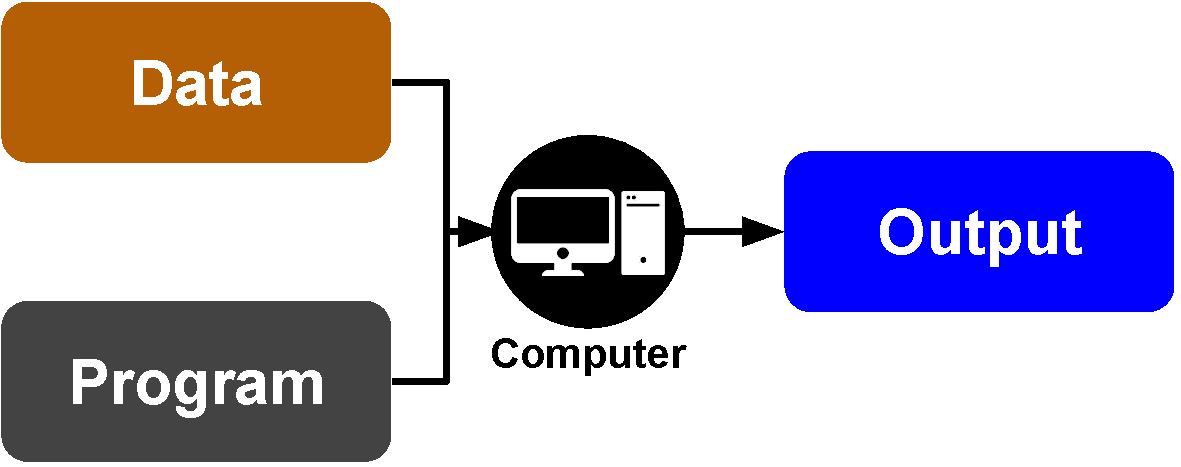
\includegraphics[width=\currprop]{figures/3_theoretical_background/shallow_learning/traditional_programming_pipeline.pdf} % + 0.19
    \caption{}
    \label{fig:traditional_programming_pipeline}
  \end{subfigure}
  \hfil % This provides the horizontal space
  \begin{subfigure}[c]{0.48\columnwidth} % Reduced width
    \centering
    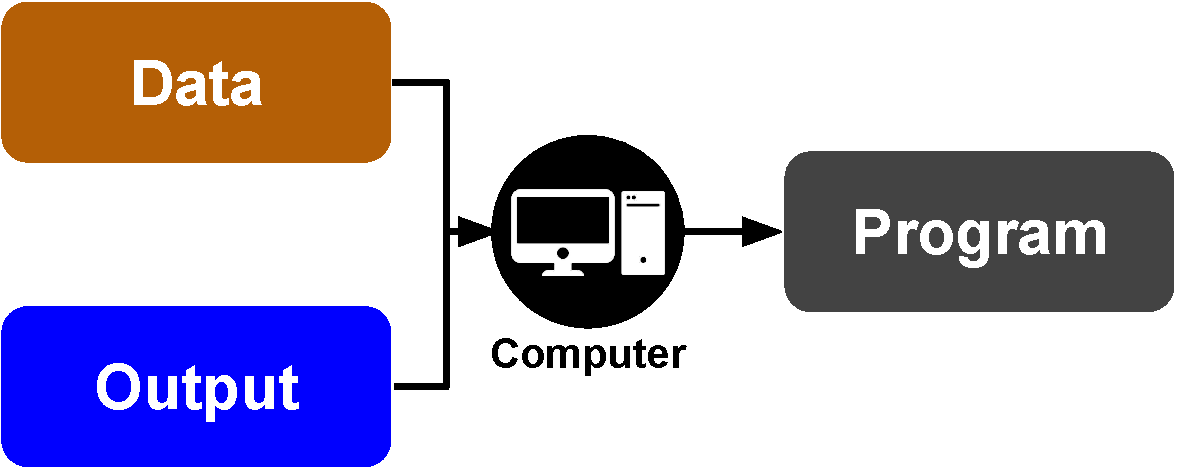
\includegraphics[clip,width=\currprop]{figures/3_theoretical_background/shallow_learning/machine_learning_pipeline.pdf}
    \caption{}
    \label{fig:machine_learning_pipeline}
  \end{subfigure}

  \fignote{(a) shows Classical Programming paradigm, while (b) shows the new Machine Learning paradigm.}
\end{figure}

\subsection{Shallow Learning models}

In this context, \ac{SL} is a \ac{ML} approach that works well for tabular data, but requires preprocessing steps for unstructured data (such as images, videos, texts, or \ac{SITS}) converting them into tabular data, a complete subfield called Feature Engineering \cite{zheng2018feature}. In addition to the requirement for handcrafted features, such models are generally older and less complex compared to current models, and the name ``shallow'' contrasts with \ac{DL}, which will be explained in more detail in Section \ref{sec:deep_learning}. Also, \ac{SL} models often require less data for training and are faster to train and implement, as well as being more interpretable, which makes it easier to understand how decisions are made by the model. However, to use them, it is necessary to choose those handcrafted features (extraction and selection), which can be challenging, especially in areas such as \ac{CV} and \ac{RS}.

\subsubsection{K-Nearest Neighbor (KNN)}

\acf{KNN} is an \ac{SL} classification model based on the principle that similar instances in a dataset tend to be located close to each other in the feature space space \citep{cover1967nearest}. Unlike other models that construct an explicit mathematical function during training, \ac{KNN} is classified as a lazy learner, as it does not generate a discriminative model in advance; instead, it stores the entire training dataset and postpones computational processing until the moment of inference. 

The algorithm's operation is based on calculating the distance between the sample to be classified and all examples in the training set -- usually the Euclidean distance, although other metrics such as Manhattan or Minkowski can be applied. The model selects the $K$ closest neighbors and defines the class of the new object by majority vote (see Figure \ref{fig:knn}). In the context of regression, \ac{KNN} estimates the output value using the arithmetic or weighted average of the values of the $K$ neighbors. However, its computational search cost increases linearly with the number of samples ($O(n)$) and is highly sensitive to the scale of the variables, requiring normalization steps and, often, dimensionality reduction techniques (such as PCA).

\begin{figure}[ht!]
    \centering
    \caption{Diagram of a K-nearest neighbor model.}
    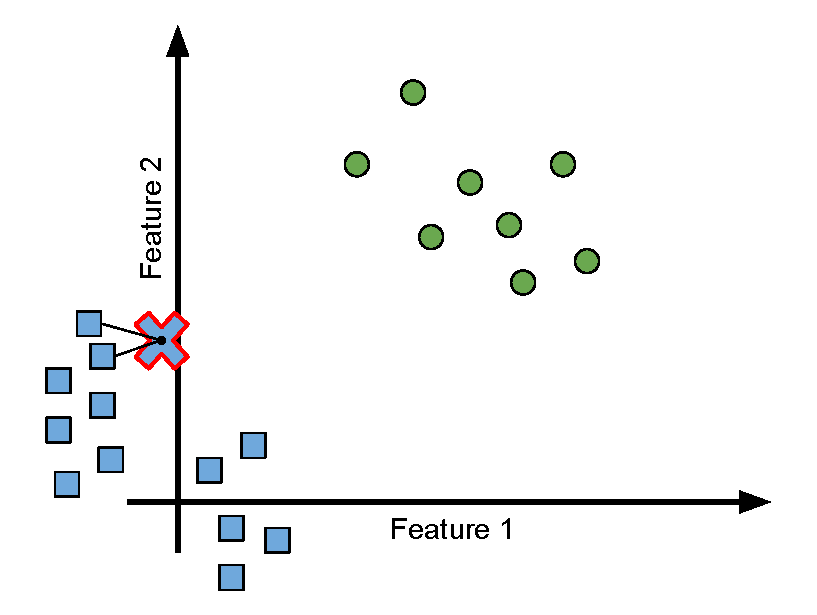
\includegraphics[width=.7\linewidth]{figures/3_theoretical_background/shallow_learning/knn.pdf}
    \fignote{One should notice that, in this model K=2 so, when a prediction sample is given (the X in the figure), the two most near training samples classes are verified, than their class will be assigned to the given prediction sample.}
    \label{fig:knn}
\end{figure}

\Ac{KNN} is widely used as a test for \ac{SSL} pre-training due to its simplicity and ability to provide a quick assessment of the quality of the generated embeddings, being retrained at each new pre-training epoch.

\subsubsection{Support Vector Machine (SVM)}

\Acf{SVM} is a widely used supervised learning algorithm for classification and regression tasks \citep{boser1992training}. SVM works by finding the optimal hyperplane that separates different classes of data in feature space, maximizing the margin between classes (see the Figure \ref{fig:svm}). In cases where the data is not linearly separable (such as spectral bands in \ac{RS}), \ac{SVM} can use the ``kernel trick'' to transform the data into a higher-dimensional space where linear separation is possible. \ac{SVM} is known for its effectiveness on high-dimensional datasets and its robustness against overfitting, especially when configured with the correct parameters.

\begin{figure}[ht!]
    \centering
    \caption{Diagram of a Support Vector Machine model.}
    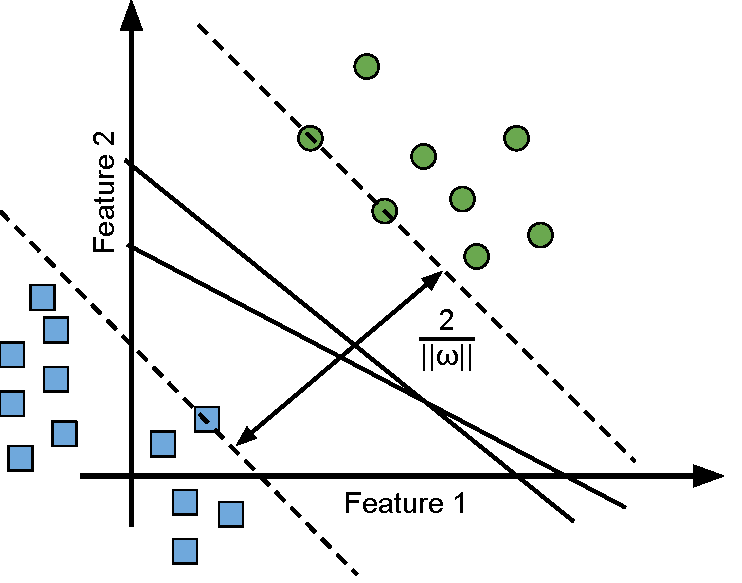
\includegraphics[width=.7\linewidth]{figures/3_theoretical_background/shallow_learning/svm.pdf}
    \label{fig:svm}
\end{figure}

The main idea behind the kernel trick is to map the input data to a higher-dimensional space where linear separation between classes can be achieved. Instead of explicitly calculating the coordinates of the data in this higher-dimensional space, the kernel trick allows us to directly calculate the inner products between the data vectors in the original space using specific kernel functions. The most common kernels include the Linear Kernel (for data that is already linearly separable), the Polynomial Kernel (which introduces curvature), and, notably, the Radial Basis Function (RBF) Kernel, which is one of the most widely used due to its effectiveness in dealing with complex separations in \ac{RS}.

Despite its theoretical robustness and good performance on many datasets, \ac{SVM} presents some practical challenges. First, the high computational cost and training time can be significant, especially with increasing data volume (very large datasets, such as pixels of multiespectral satellite images). Training time generally scales between $O(n^2)$ and $O(n^3)$ (where $n$ is the number of training samples), making it less efficient for large volumes of raw data than, for example, \ac{RF}. Second, \ac{SVM} performance is highly sensitive to the choice and adjustment of Kernel parameters (hyperparameters) and the penalty parameter ($C$). As such, \ac{SVM} usually requires several different long training sessions (with different hyperparameters), making the model quite costly.

\subsubsection{Random Forest (RF)}
\label{sec:rf}

\Acf{RF} is a \ac{SL} model that combines multiple simpler models, \acf{DT}, to improve the quality and robustness of predictions \citep{breiman2001random}. A \ac{DT} (see the black bounding box in Figure \ref{fig:random_forest}) works by recursively dividing a dataset into smaller, more homogeneous subsets based on input characteristics (variables) \citep{quinlan1986induction}. Although simple and interpretable, a single \ac{DT} is often susceptible to overfitting, which means that it may perform well on training data but poorly on test data. However, on the plus side, it is one of the most interpretable models in the entire field of machine learning, precisely because it approximates the way humans think about tasks or define classes, as exemplified above.

\begin{figure}[ht!]
    \centering
    \caption{Diagram of a Random Forest model.}
    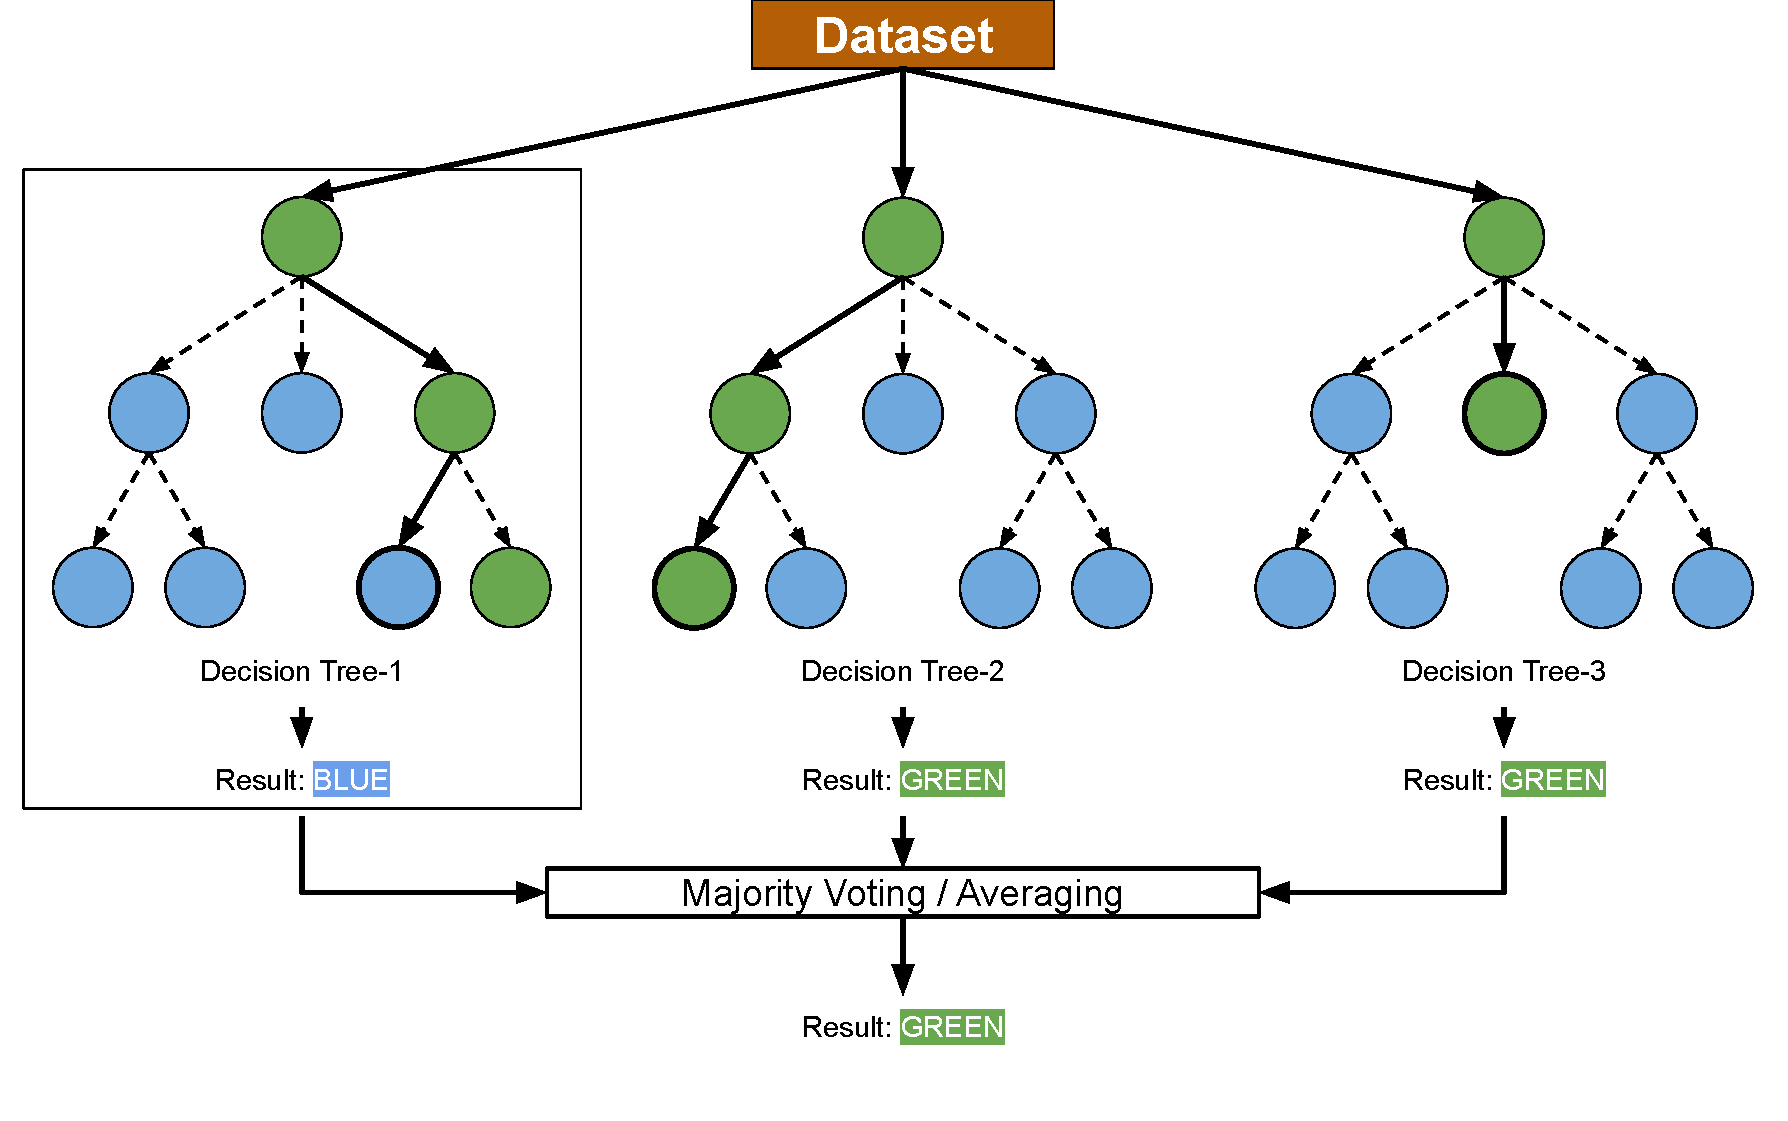
\includegraphics[width=1\linewidth]{figures/3_theoretical_background/shallow_learning/random_forest.pdf}
    \fignote{The black bounding box is highlighting a decision tree, the core subpart of a RF.}
    \label{fig:random_forest}
\end{figure}

In \ac{RS}, \ac{RF} is a classification tool that is still widely used today, mainly for \ac{LULC}. It is widely used because it does not require data preprocessing, being one of the few models that is robust to data scale. Thus, it is quite common to classify image pixels or satellite mosaics, creating thematic maps in shallow semantic segmentation. Due to its training speed and lack of preprocessing requirements, it is also a widely used model as a baseline for more advanced techniques.

\subsubsection{Gradient Boosting (GB)}

\Acf{GB} models, on the other hand, are very similar to \ac{RF} (see Section \ref{sec:rf}), as they also build multiple \ac{DT} to improve predictive performance \citep{friedman2001greedy}. However, while \ac{RF} builds trees independently and joins them together, \ac{GB} builds trees sequentially, where each new tree attempts to correct the errors of the previous trees. This process is known as boosting, and the goal is to minimize a specific loss function by iteratively adding weak models that improve the overall performance of the model.

\begin{figure}[ht!]
    \centering
    \caption{Diagram of a Gradient Boosting (GB) model.}
    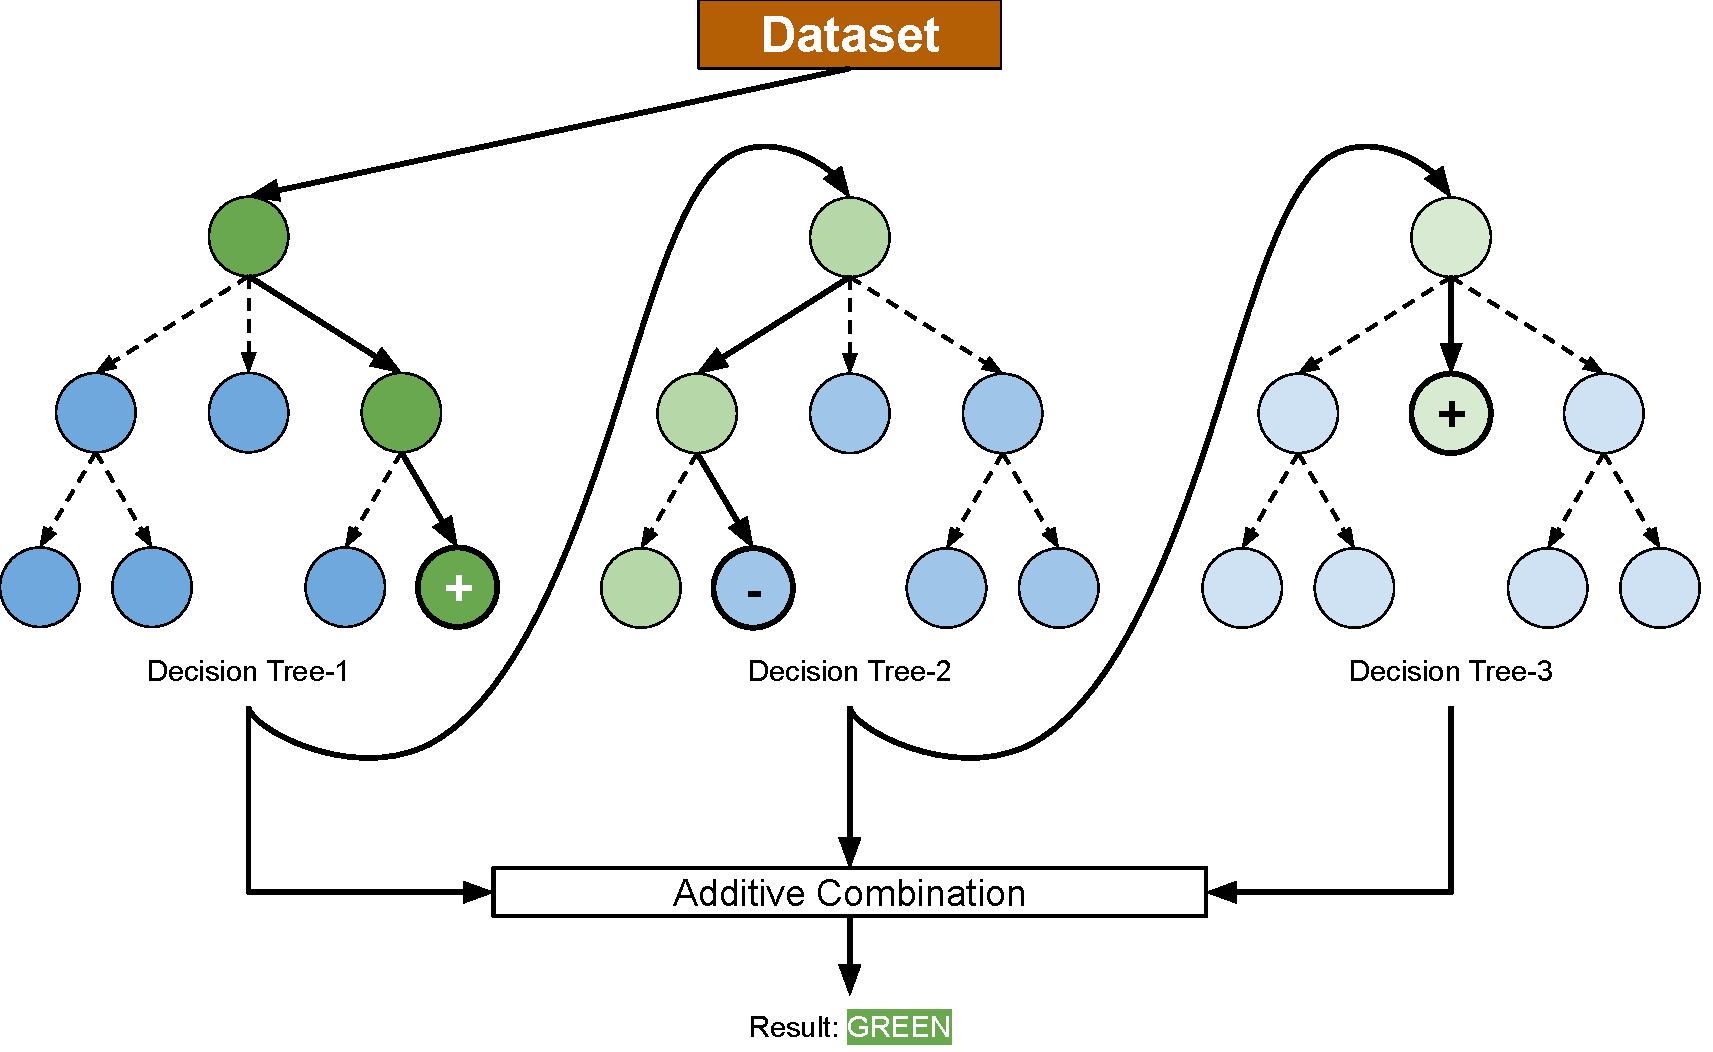
\includegraphics[width=1\linewidth]{figures/3_theoretical_background/shallow_learning/gradient_boosting.pdf}
    \fignote{One should notice that the Decision Trees refine each other's decisions.}
    \label{fig:gradient_boosting}
\end{figure}

In \ac{RS}, \ac{GB} has uses that are extremely similar to RF, functioning as a more costly
alternative - both in terms of computational cost and scientist time - but ofter with better results. Two famous implementations of \ac{GB} stand out: XGBoost and LightGBM. The main difference in standard hyperparameter optimization strategies between LightGBM and XGBoost lies in the treatment of the tree: LightGBM uses depth-based (leaf-wise) tree growth, generally resulting in deeper and more asymmetric \ac{DT} by default, while XGBoost typically uses level-wise growth, producing balanced \ac{DT}, which directly affects the standard parameters of maximum depth and number of leaves, both of which are widely used in \ac{RS}.

\subsubsection{Multi-Layer Perceptron (MLP)}
\label{sec:mlp}

The \ac{MLP} is a classic Artificial Neural Network (ANN) architecture consisting of multiple layers of fully connected neurons, i.e., each neuron in one layer is connected to all neurons in the next layer \citep{rosenblatt1958perceptron, rumelhart1986learning}. Such a model is also called a Feedforward Neural Network (FNN). The \ac{MLP} is composed of an input layer, one or more hidden layers, and an output layer. The hidden layers apply nonlinear activation functions, such as \ac{ReLU} or sigmoid, to introduce nonlinearity to the model.

\begin{figure}[ht!]
    \centering
    \caption{Diagram of a Multi-Layer Perceptron.}
    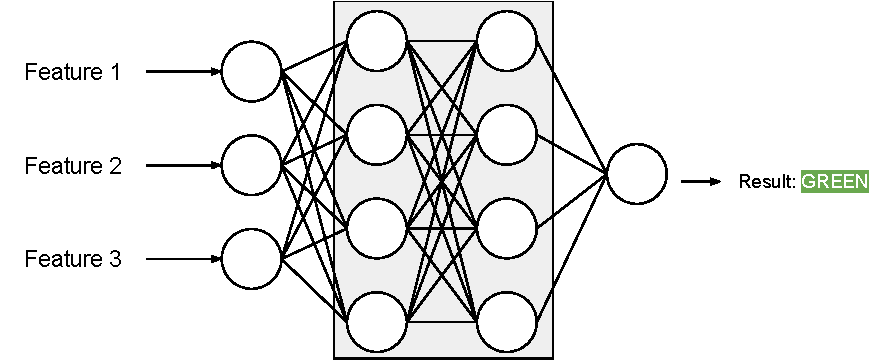
\includegraphics[width=.8\linewidth]{figures/3_theoretical_background/deep learning/mlp.pdf}
    \label{fig:mlp}
\end{figure}

Historically, \ac{MLP} represents the foundational architecture for \ac{DL} models. While deep configurations exist, simpler implementations with few hidden layers are often categorized alongside shallow methods. Today, \acs{MLP}s are still used at the end of other more complex neural networks to perform the final step of mapping the extracted features to the desired classes or output values. Also, this model is often used as baselines.

\subsubsection{K-Means}

K-Means is possibly the best known and most widely used Unsupervised \ac{SL} model \citep{macqueen1965some, lloyd1982least}. Unsupervised Learning is a \ac{ML} technique where the model is trained using an unlabeled dataset, i.e., the input examples do not have associated desired outputs. The goal of the model is to identify patterns, structures, or clusters in the data without the guidance of predefined labels. K-Means is a clustering algorithm that aims to partition a data set into K distinct groups, where each group is represented by a centroid. The algorithm works iteratively, assigning each data point to the nearest centroid and then recalculating the centroids based on the new assignments. This process continues until the assignments of the data points no longer change significantly or until a maximum number of iterations is reached.

\begin{figure}[ht!]
    \centering
    \caption{The impact of applying K-Means in a Unlabeled Dataset.}
    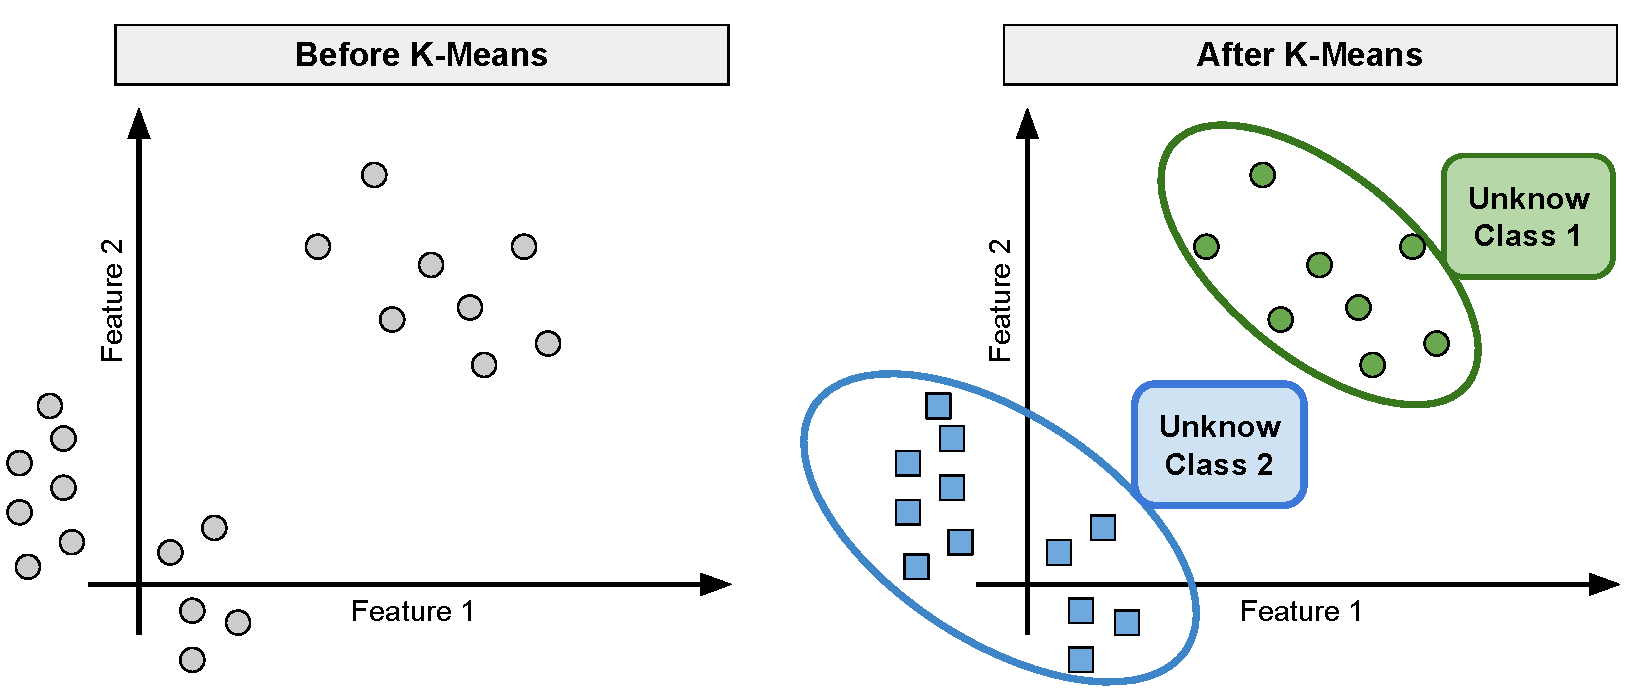
\includegraphics[width=1\linewidth]{figures/3_theoretical_background/shallow_learning/kmeans.pdf}
    \label{fig:kmeans}
\end{figure}

The big challenge is to define the value of $K$, which can be done using methods such as the elbow method or silhouette score. In \ac{RS}, K-Means is often used for image segmentation, where the goal is to group pixels with similar spectral characteristics, facilitating the identification of different types of \ac{LULC}, serving both to facilitate exploratory analysis and to assist in subsequent supervised classification tasks.

\subsubsection{Gaussian Mixture Model (GMM)}

The \acf{GMM} is an \ac{SL} unsupervised model that assumes that all data points are generated from a mixture of a finite number of Gaussian distributions with unknown parameters \citep{dempster1977maximum}. While K-Means performs hard clustering, where each point belongs exclusively to a centroid/cluster, \ac{GMM} performs soft clustering, in which the model provides the probability of a given data point belonging to each of the clusters, allowing for a more robust handling of uncertainties and class overlaps.

The model is adjusted using the Expectation-Maximization (EM) algorithm. In the Expectation step, the algorithm estimates the probability of each point belonging to each Gaussian component; in the Maximization step, the Gaussian parameters (mean, covariance, and mixture weight) are updated to maximize the likelihood of the observed data. Also similar to K-Means, to use \ac{GMM} it is necessary to determine the number of components (clusters) to be used (see Figure \ref{fig:gmm}).

\begin{figure}[ht!]
    \centering
    \caption{Diagram of a Gaussian Mixture Model.}
    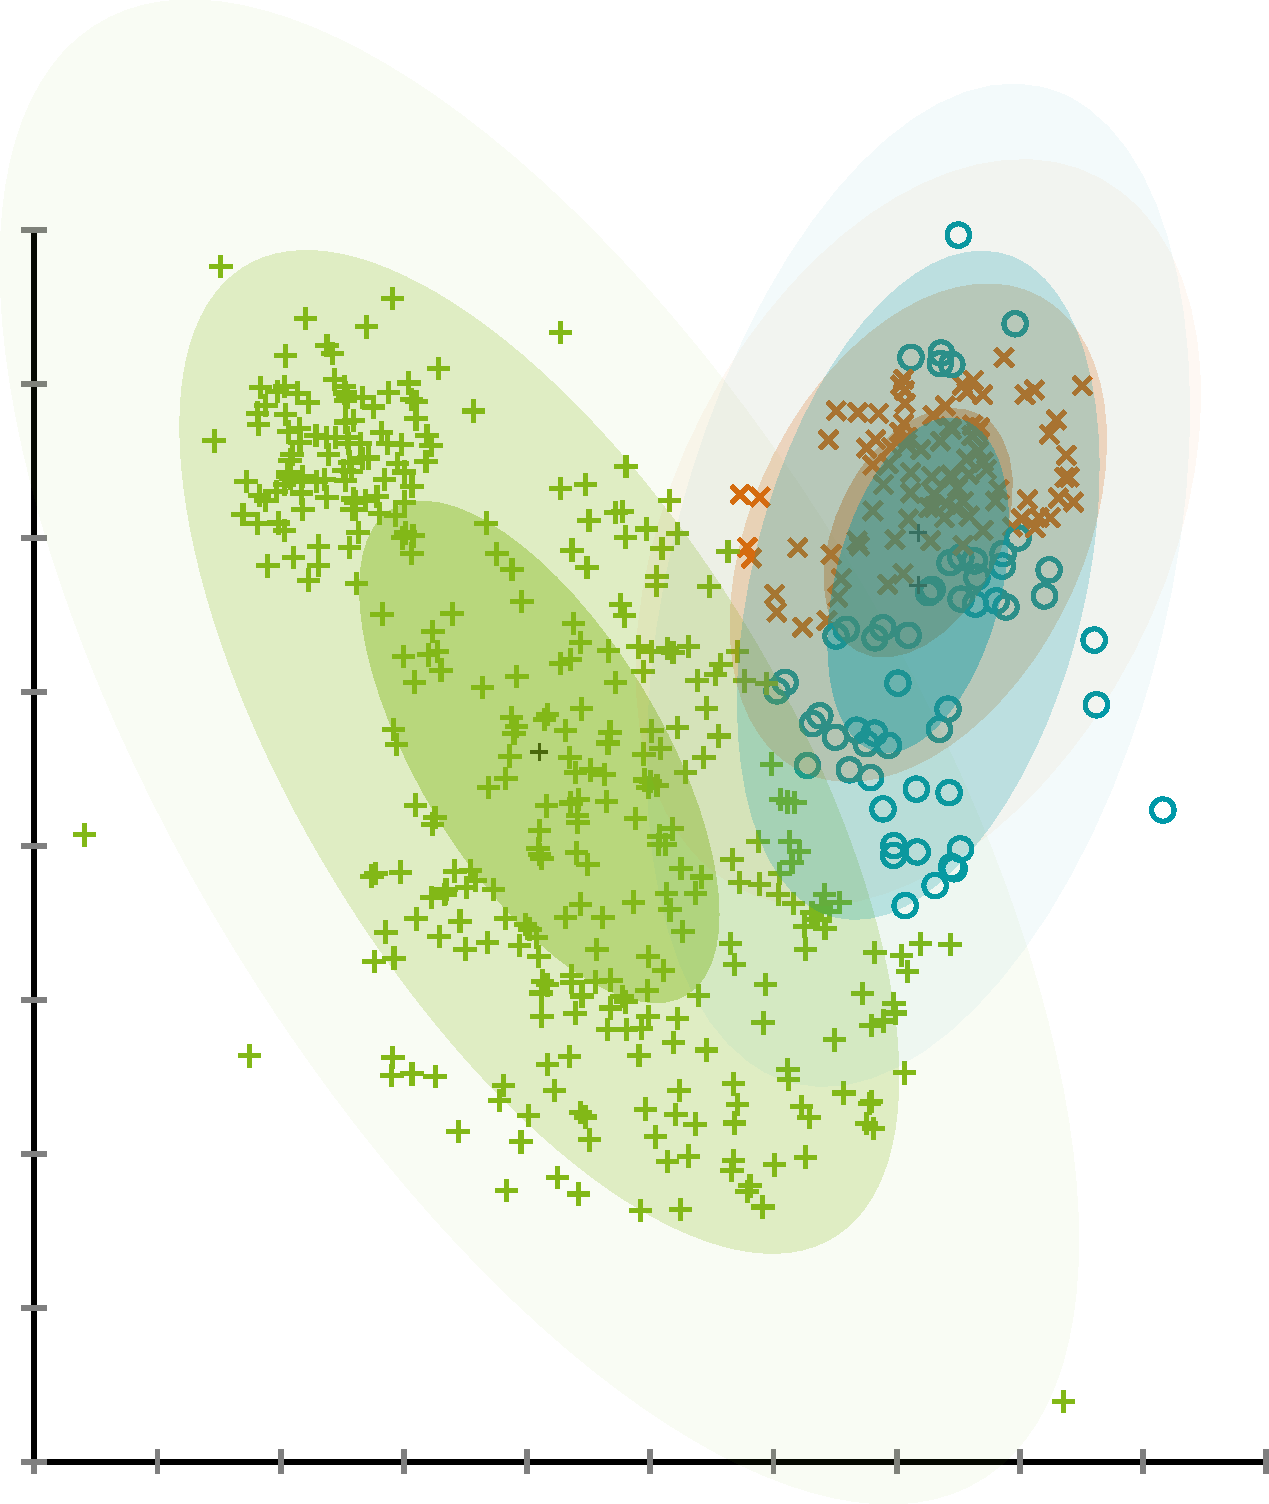
\includegraphics[width=.7\linewidth]{figures/3_theoretical_background/shallow_learning/gmm.pdf}
    \fignote{This example shows a GMM with number of components=3. Adapted from \href{https://dm.cs.tu-dortmund.de/mlbits/cluster-em-gmm-demo/}{TU Dortmund}}
    \label{fig:gmm}
\end{figure}


\subsection{Deep Learning models}
\label{sec:deep_learning}

On the other hand, \ac{DL} is a Machine Learning approach that uses latent data representations, meaning that the model itself learns to extract relevant features from raw data, eliminating the need for manual handcrafted feature extraction (with the exception, of course, of data normalization, which helps in model training convergence) \cite{bishop2023deep}. The best-known \ac{DL} models are Artificial Neural Networks (ANNs), which are composed of multiple layers of interconnected artificial neurons \cite{goodfellow2016deep}. Each neuron receives inputs, applies an activation function, and transmits the output to the neurons in the next layer. A loss function is defined to quantify the difference between the model's predictions and the actual values, and the model is trained using optimization algorithms, such as gradient descent, to adjust the weights of the connections between neurons in order to minimize this loss. In supervised learning, the most common loss functions include cross-entropy for classification and mean squared error for regression, which directly compare the model's predictions with the actual labels during training. Unsupervised techniques is also used in \ac{DL} to learn representations of data without explicit labels with different loss functions.

\subsubsection{Convolutional Neural Network (CNN)}
\label{sec:cnn}

A \ac{CNN} is a \ac{DL} model specially designed to process images \citep{lecun1989backpropagation}. \ac{CNN} are composed of convolutional layers that apply filters (or kernels) to extract local features from the input data, such as edges, textures, and spatial patterns. These layers are followed by pooling layers, which reduce the dimensionality of the data while retaining the most important features. Finally, an \ac{MLP} (see Section \ref{sec:mlp}) is generally used to perform classification or regression based on the extracted features.

\begin{figure}[ht!]
    \centering
    \caption{Diagram of a Convolutional Neural Network.}
    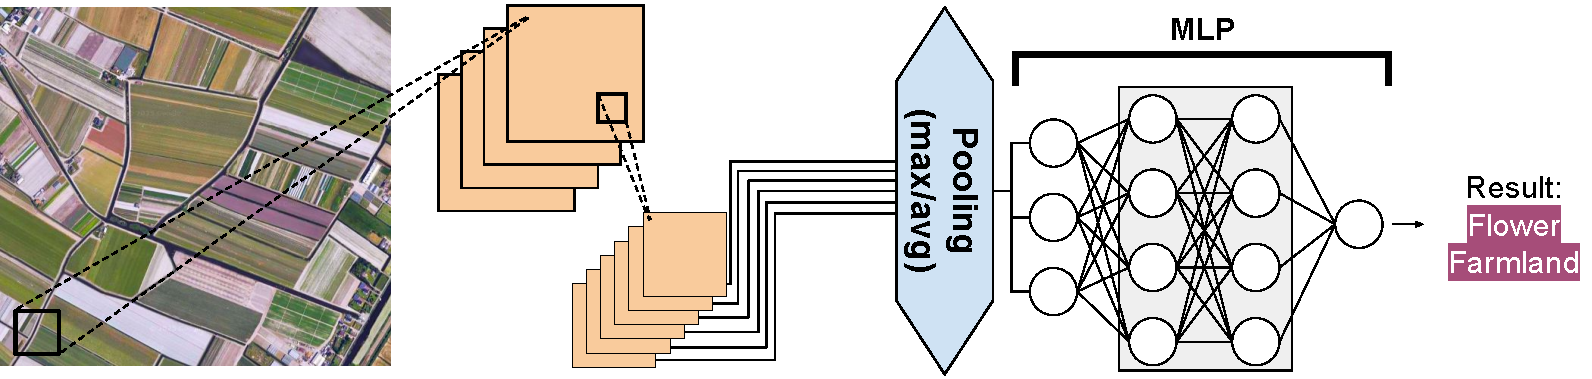
\includegraphics[width=1\linewidth]{figures/3_theoretical_background/deep learning/cnn.pdf}
    \label{fig:cnn}
\end{figure}

The motivation behind \ac{CNN} is to avoid the extremely high number of parameters that an \ac{MLP} would have when dealing with images, which generally have high dimensionality. For example, a $256\times256$ pixel Sentinel 2 image has $655360$ entries ($256 \times 256 \times 10$), which would result in millions of parameters in a typical \ac{MLP}. \acs{CNN}s allow kernels- such as Sobel and Canny kernels- to be trained and customized for each dataset, drastically reducing the number of parameters and making training possible.

The history of \acp{CNN} began with its use for character recognition \citep{lecun1989backpropagation} and the consolidation of LeNet-5 \citep{lecun2002gradient}, but it was AlexNet \citep{krizhevsky2012imagenet} that revolutionized the field by demonstrating the potential of GPUs -- which led to their widespread use throughout the field of machine learning -- and the \ac{ReLU} function in deep networks. This was followed by approaches such as VGG \citep{simonyan2014very}, focused on depth with small filters, and GoogleNet \citep{szegedy2015going}, which introduced Inception modules for multiscale processing, a technique refined in subsequent versions \citep{szegedy2016rethinking,szegedy2017inception}. A definitive milestone was ResNet \citep{he2016deep}, whose residual connections that dealt with Vanishing Gradients enabled networks with hundreds of layers, underpinning models such as ResNeXt \citep{xie2017aggregated}, based on cardinality, and DenseNet \citep{huang2017densely}, which prioritizes feature reuse (see Figure \ref{fig:cnn_hist}).

\begin{figure}[ht!]
    \centering
    \caption{Historical diagram of the evolution of Convolutional Neural Networs.}
    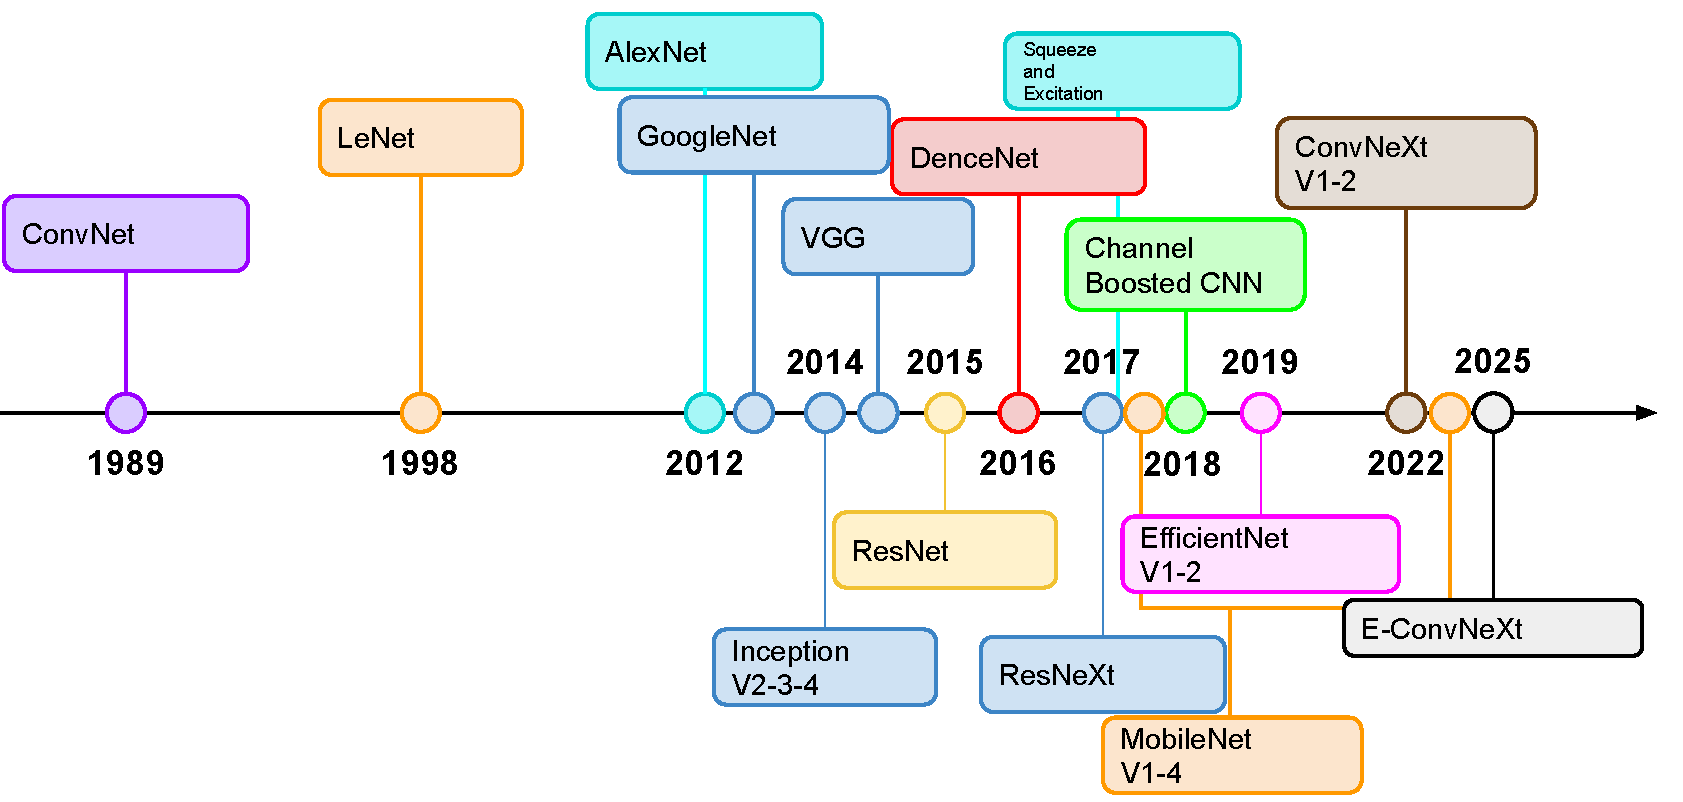
\includegraphics[width=1\linewidth]{figures/3_theoretical_background/deep learning/cnn_history.pdf}
    \label{fig:cnn_hist}
\end{figure}

Recently, efficiency has become the priority with the EfficientNet family \citep{tan2019efficientnet,tan2021efficientnetv2}, which optimized the width and depth scaling of networks. Being contemporary, the MobileNet series \citep{howard2017mobilenetsefficientconvolutionalneural,sandler2019mobilenetv2invertedresidualslinear,howard2019searchingmobilenetv3,qin2024mobilenetv4universalmodels} leveraged depthwise separable convolutions to balance latency and accuracy in resource-constrained environments. Concurrently, Squeeze-and-Excitation networks \citep{hu2019squeezeandexcitationnetworks} introduced channel-wise attention mechanisms to explicitly model interdependencies between channels, enhancing representational power with minimal computational overhead. In response to the rise of Transformers, the ConvNeXt architecture \citep{liu2022convnet} modernized \acp{CNN} with contemporary design choices, evolving to V2 \citep{woo2023convnext} with the use of masked autoencoders and to E-ConvNeXt \citep{wang2025convnext}, focused on low-resource devices. Complementarily, approaches such as Channel Boosted CNN \citep{khan2018new} explored channel diversity via transfer learning in an attempt to keep \acp{CNN} competitive in the face of new computer vision paradigms, especially in scenarios with low computational resources or little data.

\subsubsection{Semantic Segmentation Models}
\label{sec:fcn}

Some adaptions were done to convert \ac{CNN}s (see Section \ref{sec:cnn}) for semantic segmentation tasks, where the goal is to classify each pixel in an image into a specific class. One of the first adaptations, and still widely used today, is the \acf{FCN} \citep{long2015fully}. The strategy used was to replace the typical final \ac{MLP} of \ac{CNN} with deconvolution (or upsampling) layers, allowing the network to process images of any size and produce corresponding segmentation maps (see Figure \ref{fig:fcn}) .

\begin{figure}[ht!]
    \centering
    \caption{Diagram of a Fully Convolutional Network model.}
    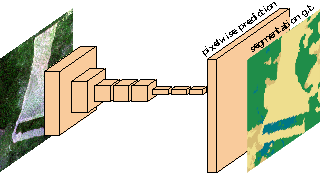
\includegraphics[width=.75\linewidth]{figures/3_theoretical_background/deep learning/fcn.pdf}
    \fignote{Adapted from Long et al \citep{long2015fullyconvolutionalnetworkssemantic}}
    \label{fig:fcn}
\end{figure}

This architecture is especially useful in \ac{RS} for LULC and Parcel Delineation applications -- as they are intrinsically semantic segmentation applications -- in addition to some uses in Crop Mapping or Crop Yielding. Furthermore, variations in which two \ac{FCN} are combined and have their embeddings concatenated are also used for Change Detection.

Aside from the FCN strategy, another common strategy for semantic segmentation networks is that of encoder-decoder networks, such as the U-Net model. U-Net was designed for biomedical image segmentation tasks, but is also possibly the most historically used \ac{DL} model in \ac{RS} \citep{ronneberger2015u}. The main innovation of U-Net is its ``U''-shaped structure, which consists of a path of reduced spatial resolution and increased number of channels (encoder) and subsequently a path of increased spatial resolution and decreased number of channels (decoder). The encoder follows a design pattern similar to that of \ac{CNN}, using blocks containing convolutional layers, \ac{ReLU} activation, and max pooling. On the other hand, the decoder is composed of upsampling and convolution layers, which help to reconstruct the spatial resolution of the image. This architecture allows the network to capture contexts of different scales while maintaining accurate spatial information. The Decision Factor of U-Net is the skip connections that link the corresponding layers of the encoder and decoder, allowing detailed information to be transferred directly to the reconstruction process, significantly improving segmentation accuracy (see Figure \ref{fig:unet}).

\begin{figure}[ht!]
    \centering
    \caption{Diagram of a U-Net model.}
    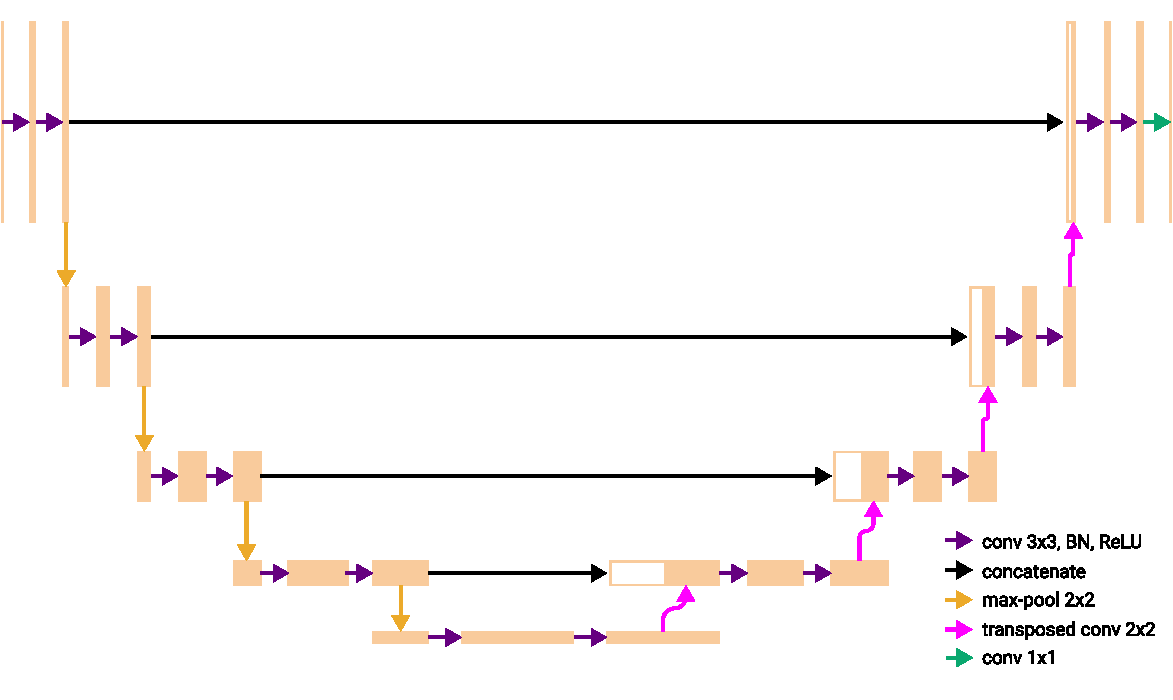
\includegraphics[width=0.8\linewidth]{figures/3_theoretical_background/deep learning/unet.pdf}
    \fignote{One should notice that the model layers ressemble a U. Adapted from \href{https://innolitics.com/articles/medical-image-segmentation-overview/}{Innolitics}}
    \label{fig:unet}
\end{figure}

Several variations of U-Net have been proposed over the years, such as U-Net++ and Attention U-Net, which introduce improvements in skip connections to increase the accuracy and efficiency of the model. In addition, there are also variations that change the encoder to classics \acs{CNN}s architectures such as ResNet or EfficientNet - without using the final \ac{MLP} (see Section \ref{sec:mlp}) - aiming to improve the model's feature extraction capability.


\subsubsection{AutoEncoder (AE)}

\Acf{AE} is a \ac{DL} architecture designed to learn compressed representations of input data, usually for dimensionality reduction or feature learning later used in another model \citep{hinton2006reducing}. An autoencoder consists of two main parts: the encoder and the decoder. The encoder maps the input data to a lower-dimensional latent space, compressing the information, while the decoder reconstructs the original data from this compressed representation (see Figure \ref{fig:autoencoder}).

\begin{figure}[ht!]
    \centering
    \caption{Diagram of a AutoEncoder model.}
    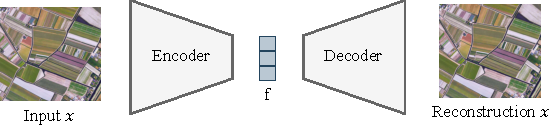
\includegraphics[width=0.85\linewidth]{figures/3_theoretical_background/deep learning/autoencoder.pdf}
    \fignote{Adapted from \href{https://uvadlc-notebooks.readthedocs.io/en/latest/tutorial_notebooks/tutorial9/AE_CIFAR10.html}{UvA Deep Learning Tutorials}}
    \label{fig:autoencoder}
\end{figure}

There are several types of autoencoders, including Denoising Autoencoders, which learn to reconstruct noisy data, and Variational Autoencoders (VAEs), which introduce a probabilistic approach to data generation - allowing, for example, the generation of data that mixes different classes. In \ac{RS}, autoencoders are often used for pretraining models, but this topic will be better addressed in Section \ref{sec:ssl_contextualization}.

\subsubsection{Generative Adversarial Network (GAN)}

\Acf{GAN} is a DL architecture composed of two neural models that compete with each other: the generator and the discriminator. The generator creates synthetic data from a random input, while the discriminator attempts to distinguish between real and generated data. During training, both models are trained, the generator learns to create increasingly realistic data, while the discriminator becomes more effective at identifying false data (see Figure \ref{fig:gan}). The convergence of this process is theoretically guaranteed by the ``Nash equilibrium'', in which both the generator and the discriminator have no significant gains in changing their strategy, although this is usually only seen approximately in practice.

\begin{figure}[ht!]
    \centering
    \caption{Diagram of a Generative Adversarial Network model.}
    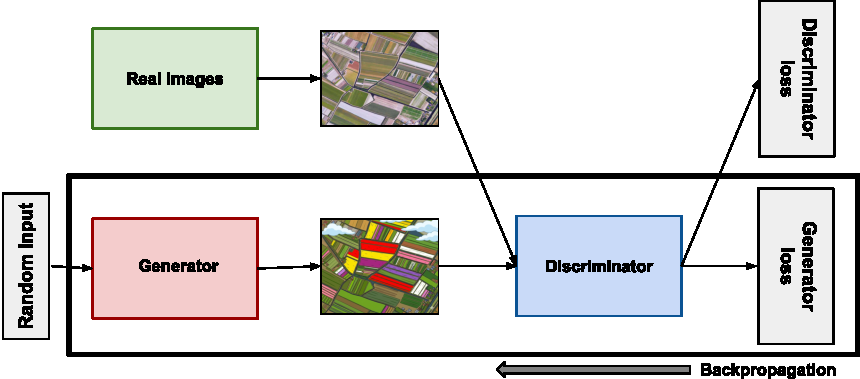
\includegraphics[width=1\linewidth]{figures/3_theoretical_background/deep learning/gan.pdf}
    \fignote{Adapted from \href{https://developers.google.com/machine-learning/gan/generator}{Google Developers}}
    \label{fig:gan}
\end{figure}

In \ac{RS}, \acs{GAN}s are used for various applications, such as synthetic image generation, image translation between different domains (e.g., from radar images to optical images), and especially for super-resolution of satellite images \citep{goodfellow2014generative}. In addition, \acs{GAN}s are also used to augment limited datasets by generating additional samples that help improve the performance of supervised models, which is useful for scenarios with very little data, as is often the case with Crop Yielding. However, \acs{GAN}s are known to potentially generate artifacts in the images they produce, which can be a challenge in applications that require high fidelity, in addition to the impossibility of auditing the generated data, making them difficult to use in applications such as deforestation Change Detection.


\subsubsection{Recurrent Neural Network (RNN)}
\label{sec:rnn}

A \ac{RNN} is a \ac{DL} model designed to handle sequential data, used in \ac{RS} for time series processing, whether pixels or images, through hybrid models with \ac{CNN}. \acs{RNN}s have recurrent connections that allow information from previous steps in the sequence to be retained and used to influence predictions in subsequent steps.

\acs{RNN}s work through a hidden state ($h_t$) that is updated at each step of the sequence ($x_t$), allowing the model to capture temporal dependencies in the data and produce an output ($y_t$) at each step (see Figure \ref{fig:rnn}). However, they suffer from the problem of gradient vanishing, which makes it difficult to learn long-term dependencies in long sequences.

\begin{figure}[ht!]
    \centering
    \caption{Diagram of a Recurrent Neural Network model.}
    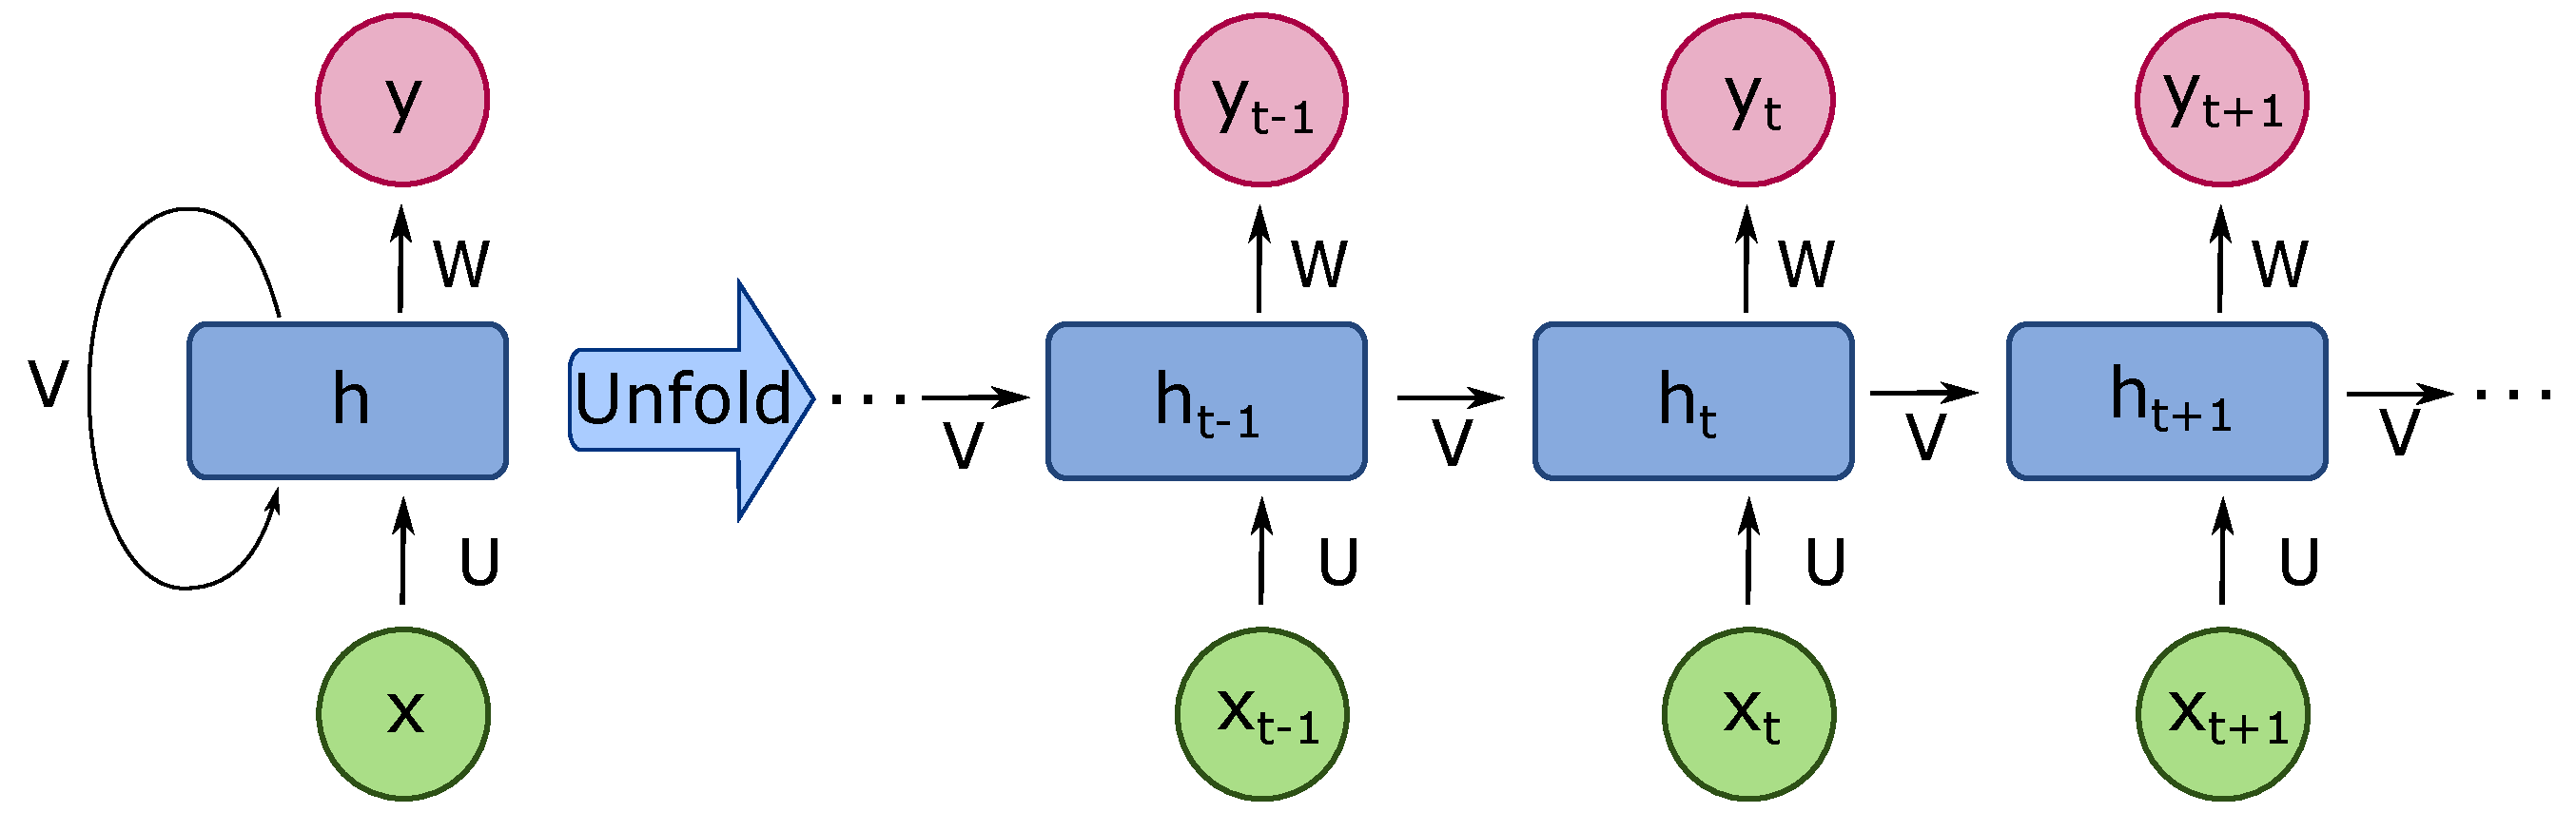
\includegraphics[width=.7\linewidth]{figures/3_theoretical_background/deep learning/rnn.pdf}
    \fignote{Adapted from \href{https://commons.wikimedia.org/wiki/File:Recurrent_neural_network_unfold.svg}{RNN - Wikimedia}}
    \label{fig:rnn}
\end{figure}

\subsubsection{Long Short-Term Memory (LSTM)}
\label{sec:lstm}

A \ac{LSTM} is an evolution of \ac{RNN} designed to mitigate vanishing gradients, allowing the model to capture long-term dependencies in sequential data \citep{graves2012long}. \acs{LSTM}s introduce a special cell structure (see Figure \ref{fig:lstm}) that includes input, forget, and output gates, allowing the model to control the flow of information and retain or discard information as needed.

\begin{figure}[ht!]
    \centering
    \caption{Diagarm of a Long Short-Term Memory model.}
    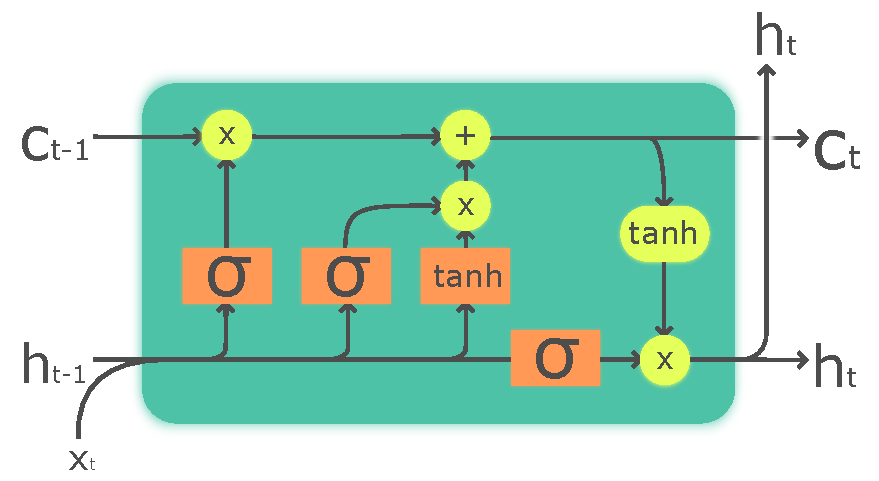
\includegraphics[width=.7\linewidth]{figures/3_theoretical_background/deep learning/lstm.pdf}
    \fignote{Adapted from \href{https://commons.wikimedia.org/wiki/File:The_LSTM_Cell.svg}{LSTM - Wikimedia}}
    \label{fig:lstm}
\end{figure}

The basis of the \ac{LSTM} is the cell state ($C_t$), a data line that runs through the entire chain and is protected by three gates that regulate what enters and what leaves. The Forget Gate ($\sigma$) decides, based on the current input ($x_t$) and the previous hidden state ($h_{t-1}$), which information from $C_{t-1}$ will be discarded or retained. Next, the Input Gate (composed of a Sigmoid $\sigma$ and a $\tanh$) determines which new data is important and adds it to the state cell. The new cell state ($C_t$) is then a combination of the old memory (filtered by the Forgetting Gate) and the new information (added by the Input Gate). Finally, the Output Gate ($\sigma$) decides which parts of $C_t$ (scaled by a tanh function) will be exposed as the hidden state ($h_t$) for the next time step, which is the actual output of the \ac{LSTM} unit to the subsequent layer and the next time step, completing the memory and prediction cycle.

A common variation of this architecture is the \acf{GRU}, which simplifies the LSTM by merging the forget and input gates into a single ``update gate'' and combining the cell state and hidden state \citep{cho2014learning}. This results in a more computationally efficient model with fewer parameters while maintaining similar performance in many tasks. Furthermore, the \acf{BiGRU} enhances this by processing the sequence in both forward and backward directions simultaneously \citep{schuster1997bidirectional}. This allows the model to capture context from both past and future states at any given time point, which is particularly useful for understanding the complete temporal evolution of a signal.

In \ac{RS}, \acs{LSTM}s and \acs{GRU}s have already been used for Crop Classification \citep{russwurm2023end} and Crop Yielding \citep{cheng2022wheat,jeong2022predicting}, due to the nature of time series in both applications. They are usually used pixel by pixel, i.e., each time series for each pixel is processed individually.

\subsubsection{Transformer}
\label{sec:transformer}

Transformer is a DL architecture originally developed for \acs{NLP}s tasks \citep{vaswani2017attention}, but which has been adapted for several other areas, including computer vision. This architecture has revolutionized the field of \ac{DL} due to its ability to capture long-range dependencies in sequential data, forming the basis for the construction of both commercial \acs{LLM}s such as ChatGPT \citep{openai2024gpt4technicalreport} and open source models such as Gemma \citep{gemmateam2025gemma3technicalreport}.

\begin{figure}[ht!]
    \centering
    \caption{Diagram of a Transformer model.}
    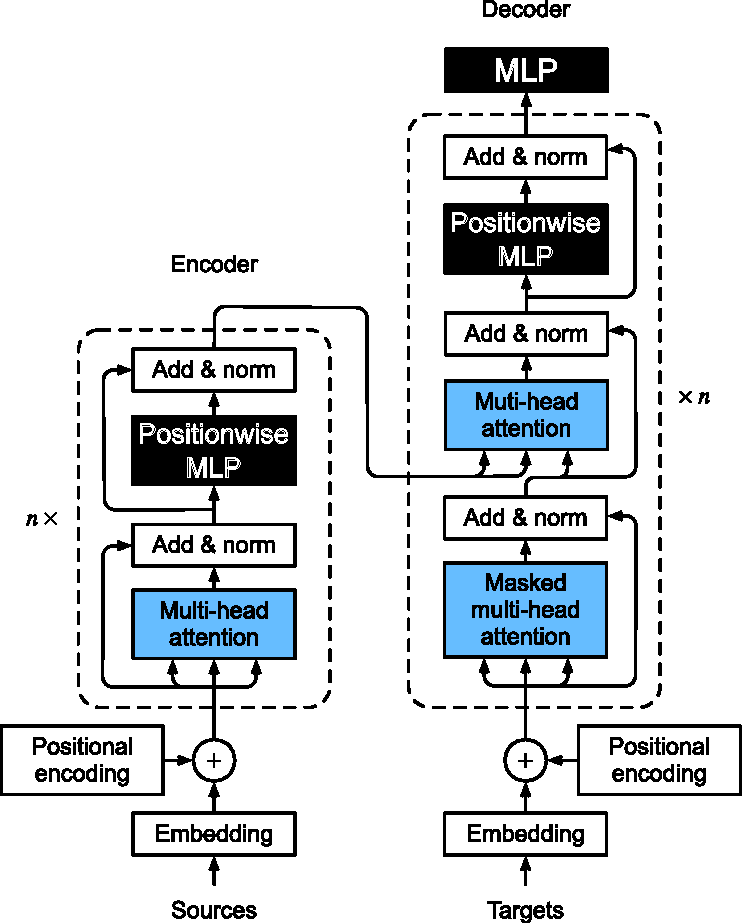
\includegraphics[width=0.7\linewidth]{figures/3_theoretical_background/deep learning/transformer.pdf}
    \fignote{Adapted from \href{https://pt.d2l.ai/chapter_attention-mechanisms/transformer.html/}{Dive into Deep Learning}}
    \label{fig:transformer}
\end{figure}

The model works by converting and processing data sequences through two interconnected structures, the Encoder (left) and the Decoder (right), which operate in $N$ repeated layers. The process begins by converting the inputs and targets into embeddings that are added (or concatenated, depending on the implementation) to a positional encoding to preserve the order of the elements. In the Encoder, Multi-head attention mechanisms simultaneously analyze the relationships between all parts of the input to create a rich representation of the context, which is refined by MLPs and normalizations for each point in the series. This contextualized representation is then sent to the Decoder, which combines the history of what has already been generated (using Masked multi-head attention to prevent access to future words) with the information coming from the Encoder, processing everything to generate the probability of the next output through a final \ac{CNN} (see graphically in Figure \ref{fig:transformer}).

Transformers were used in \ac{RS}, especially through some variations, such as the Vision Transformer (ViT) \citep{lin2023mmst} and the adapted \ac{BERT} \citep{shravan2024sits}, which will be explained later. In addition, the attention mechanism introduced by Transformers has been incorporated into several \ac{DL} architectures to improve the ability to capture spatial and temporal dependencies in \ac{RS} data.

\subsubsection{Vision Transformer (ViT)}

\Acf{ViT} is an adaptation of the Transformer architecture (see Setion \ref{sec:transformer}) for computer vision tasks such as image classification and semantic segmentation \citep{dosovitskiy2020image}. \ac{ViT} divides an image into small patches (e.g., $16\times16$ pixels), which are then flattened and transformed into embeddings, similar to words in \ac{NLP}. These embeddings are summed (or concatenated) with a positional encoding to preserve the spatial information of the patches before being fed into the Transformer model. The rest of the architecture follows the Transformer pattern, with Multi-head attention layers and \ac{MLP}s to process the embeddings of the patches and capture the relationships between them (see Figure \ref{fig:vit}), however, since the goal is not to generate a new image, the decoder is not used (which makes the architecture a subclass of Transformers called ``encoder-only'').


\begin{figure}[ht!]
    \centering
    \caption{Diagram of a Vision Transformer model.}
    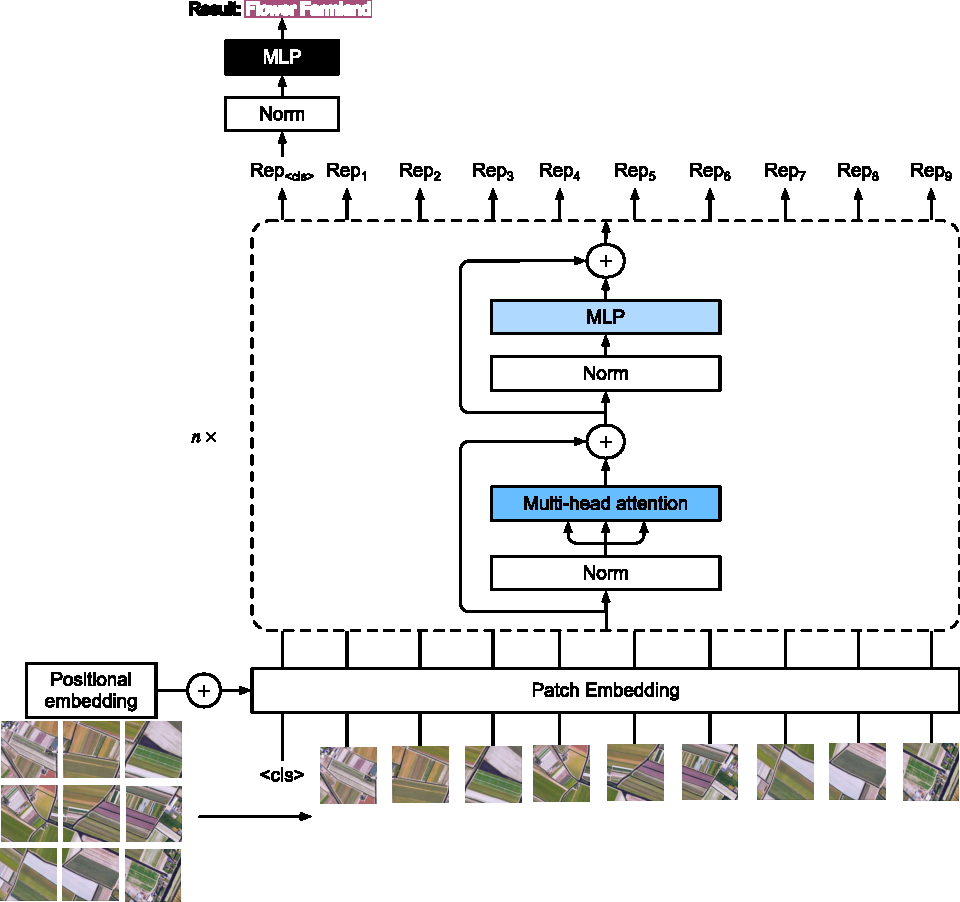
\includegraphics[width=0.7\linewidth]{figures/3_theoretical_background/deep learning/vit.pdf}
    \fignote{Adapted from \href{https://d2l.ai/chapter_attention-mechanisms-and-transformers/vision-transformer.html}{Dive into Deep Learning}}
    \label{fig:vit}
\end{figure}

Several variations of \ac{ViT} have been proposed, such as Swin Transformer, which introduces hierarchical attention mechanisms to improve the ability to capture features at different scales called Shifted windows, much like what \ac{CNN} do with their convolutional and pooling layers. The central idea is to subdivide the image several times, but each subdivision has its grid shifted relative to the previous one, allowing the model to capture both local and global features efficiently. A variation widely used in \ac{RS} is SwinNet, which combines the Swin Transformer as an encoder with an \ac{FCN}-based decoder (see Section \ref{sec:fcn}) to perform semantic segmentation.

\subsubsection{Bidirectional Encoder Representations from Transformers (BERT)}

\Acf{BERT} is a \ac{DL} model based on the Transformer architecture (see Section \ref{sec:transformer}) designed for NLP tasks \citep{devlin2019bert}. \ac{BERT} is trained using an unsupervised pre-training approach, where the model learns to predict masked words in a sentence (Masked Language Modeling) and to predict the next sentence in a pair of sentences (Next Sentence Prediction). It is known that predicting the next word is not necessary \citep{liu2019roberta}. This approach allows \ac{BERT} to capture the bidirectional context of words, considering both the context to the left and right of a word in a sentence. Subsequently, the model can be fine-tuned for a specific task, such as grammatical classification using less labeled data (see Figure \ref{fig:bert}). Note that details about \ac{SSL} pre-training, which is the case with BERT, will be better addressed in Section \ref{sec:ssl_contextualization} (the BERT pre-training, which is a Masked Modeling pre-training, it is discussed in details in Section \ref{sec:ssl_mim}).

\begin{figure}[ht!]
    \centering
    \caption{Diagram of a Bidirectional Encoder Representations from Transformers model.}
    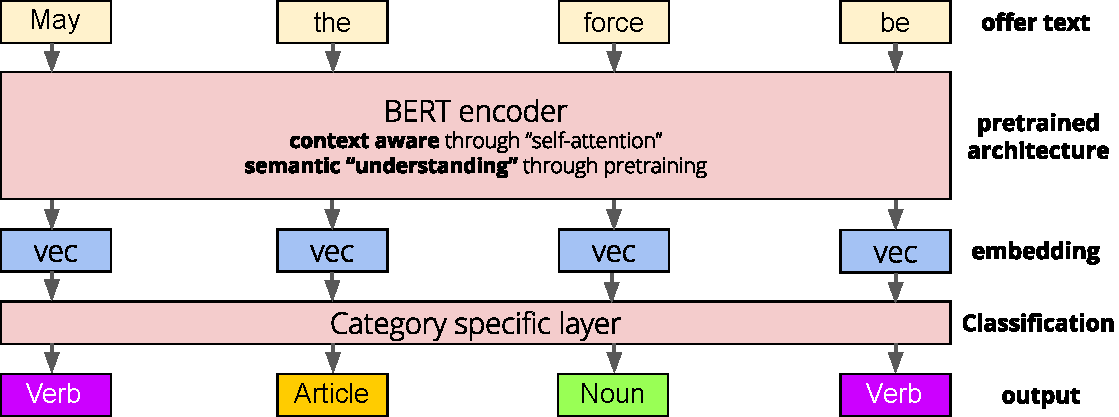
\includegraphics[width=.85\linewidth]{figures/3_theoretical_background/deep learning/bert.pdf}
    \fignote{Adapted from \href{https://dida.do/projects/numeric-attribute-extraction-from-product-descriptions}{Dida.do}}
    \label{fig:bert}
\end{figure}

Although \ac{BERT} was designed to handle \ac{NLP} data, its basic idea of Bidirectional Encoder has been adapted for other purposes such as DNA analysis \citep{zhou2025dnabert}, protein analysis \citep{brandes2022proteinbert}, and item recommendation \cite{sun2019bert4rec}. In Remote Sensing, variations of \ac{BERT} have been adapted to process \ac{SITS}, using spectral bands linearly projected directly into the \ac{BERT} Encoder.

\subsubsection{Mamba and the post-Transformer question}

Although Transformers (see Section \ref{sec:transformer}) have established the state of the art in several tasks, their architecture presents a fundamental limitation: the computational and memory complexity of the self-attention mechanism scales quadratically ($O(L^2)$) with respect to the sequence length $L$. There are even ethical discussions about the environmental impacts caused by LLMs, which almost entirely use Transformers. Which model performs as well as a Transformer but is linear ($(O(L))$) or linear-logarithmic ($(O(L\times \log L))$) is perhaps the major current question in the field of Machine Learning, with the other major question being whether such a model can even exist.

One attempt to address this is through state-space models (SSMs), with the Mamba model as its main representative. Mamba introduces a selection mechanism that allows the model to filter out irrelevant information and focus on specific contextual data, operating with linear complexity ($O(L)$).

\begin{figure}[ht!]
    \centering
    \caption{Diagram of a Mamba model.}
    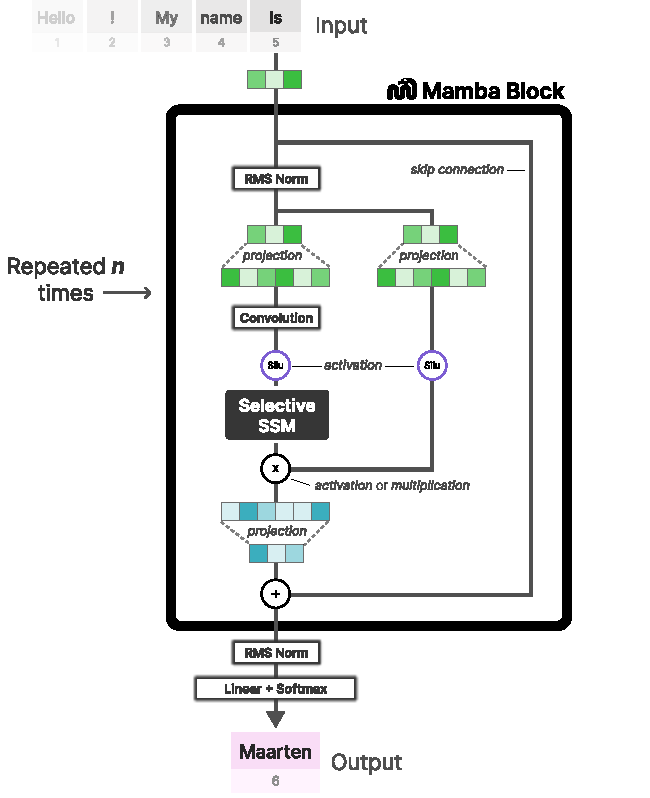
\includegraphics[width=0.75\linewidth]{figures/3_theoretical_background/deep learning/mamba.pdf}
    \fignote{Adapted from \href{https://www.maartengrootendorst.com/blog/mamba/}{
Maarten Grootendorst Blog}}
    \label{fig:mamba}
\end{figure}

The Mamba architecture is based on Selective State Space Models (S6), which allow model parameters to be functions of the input, giving it a contextual reasoning capability comparable to that of Transformers. In the field of computer vision, this approach gave rise to Vision Mamba (Vim) \citep{zhu2024vision} and VMamba \citep{liu2024vmamba}, which adapt linear scanning to two-dimensional data through the Cross-Scan Module, allowing the model to capture spatial dependencies in images without the high cost of global attention.
\section{Self-Supervised Representation Learning}
\label{sec:ssl_contextualization}

% \fromsurvey{In a scenario where the efficacy of transfer learning via fine-tuning from pretrained supervised networks is limited due to geographical domain shift \citep{nyborg2022timematch}, more robust strategies are required, such as knowledge distillation \citep{bazzi2020distilling}, domain adaptation \citep{wang2021phenology} or self-supervised learning \citep{yuan2020self,yuan2022sits,xu2024self}. This is aggravated by the lack of vast labeled datasets (see Table \ref{tab:context_labeled_datasets}), which prompted research in the field of Deep Learning for \ac{RS} seems to move towards unsupervised representation learning. In this sense, Foundational Models (FMs) are one of the most prominent family of representational methods, capable of learning richer representations from multi-modal data, enabling zero-shot predictions on a variety of tasks. FMs seem better suited for remote sensing tasks due to the lack of labeled data \citep{huo2025remote}, but there are many challenges, including data acquisition, training efficiency, data shift, and practical application challenges to use FMs in real-world scenarios \citep{yin2025fms}.}

%\fromsurvey{As described by \citep{liu2021self}, the two most common ways of computing such representations directly from unlabeled data are: (i) generative modeling; and (ii) self-supervision. In the remaining sections of this manuscript, we focus on the latter approach and its application to agricultural tasks.}


\Acf{SSL} \fromsurvey{consists of extracting supervision signals from unlabeled data, usually widely available in \ac{RS}. These procedurally computed labels are then used for pretraining learning models, which can be fine-tuned for downstream tasks using smaller amounts of labeled data \citep{balestriero2023cookbookselfsupervisedlearning}. Several visual \ac{SSL} methods \citep{he2021maskedautoencodersscalablevision} are inspired by techniques used in the pretraining phases of \acs{LLM}s such as \ac{BERT} \citep{devlin2019bert}, wherein the model is trained to recover masked words from the context of neighboring words.}

It is well known in the literature that Transfer Learning between supervised trainings does not work very well for \ac{RS}, given that the models do not generalize well between different regions, especially in agriculture, since there are climatological, soil, and even subspecies differences, where the same crop class has different subspecies for each region. Furthermore, supervised datasets are scarce (as demonstrated in \autoref{tab:context_labeled_datasets}). Therefore, \ac{SSL} proves to be a particularly useful tool for agricultural \ac{RS}, considering all these problems described, in addition to the abundance of unlabeled data, since satellites are constantly acquiring data, and there are several publicly available missions (as demonstrated in \autoref{tab:context-satellites}), plus the main characteristic of \ac{SSL} of learning intrinsic features of the target data.

\newcommand{\figscale}{0.5}

\begin{figure}[ht!]
    \centering
    \caption{Overview of the self-supervised pretraining and finetuning process.}
    \begin{subfigure}[c]{0.975\columnwidth}
        \centering
        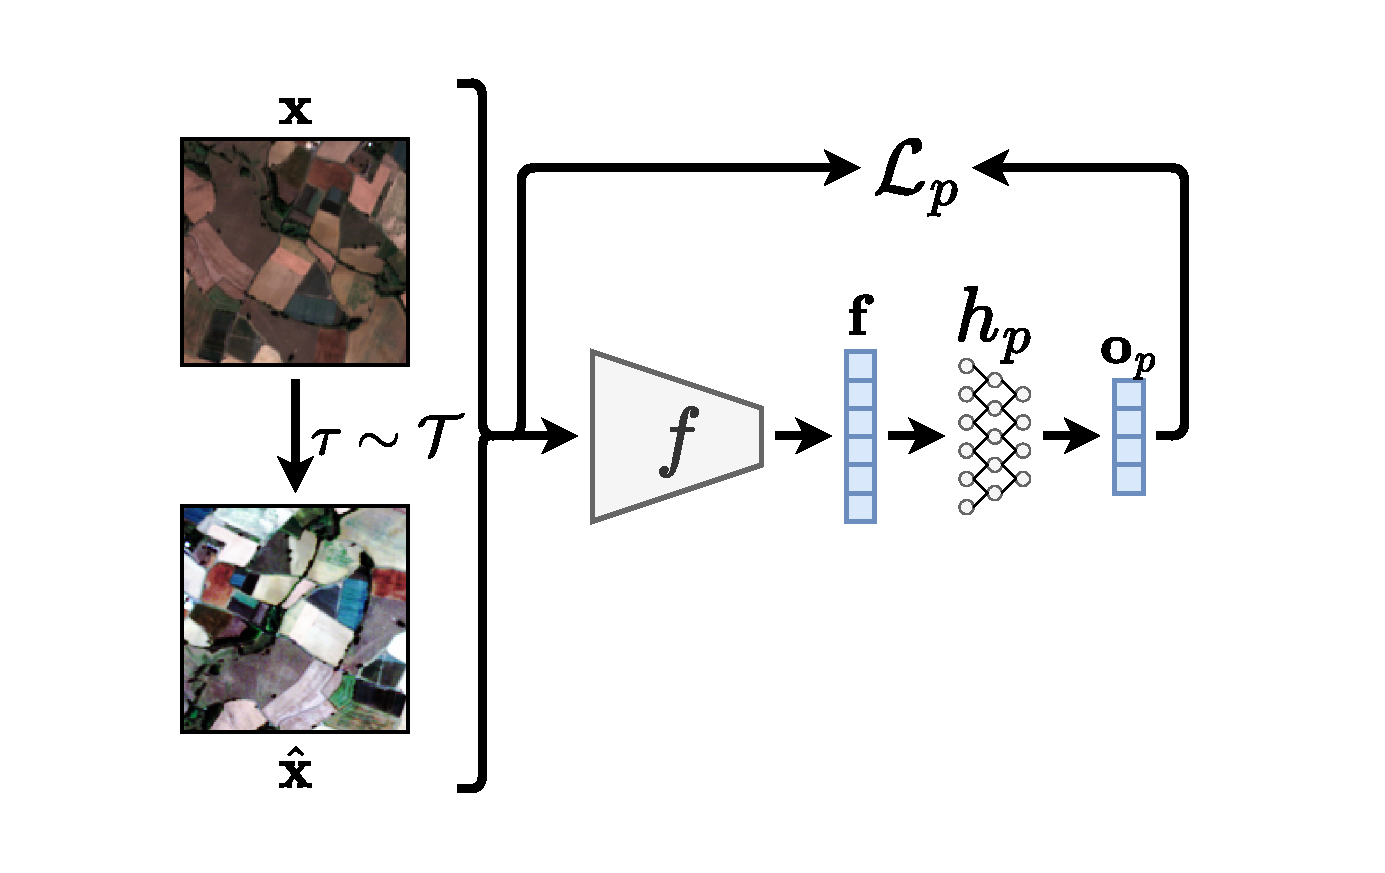
\includegraphics[clip,trim=1.15in 0.45in 0.45in 0.45in,scale=\figscale]{figures/3_theoretical_background/ssl/representation_learning_pre-training.pdf}
        \caption{\fromsurvey{}}
        \label{fig:ssl_overview_pre-training}
    \end{subfigure}
    \\
    \begin{subfigure}[c]{0.975\columnwidth}
        \centering
        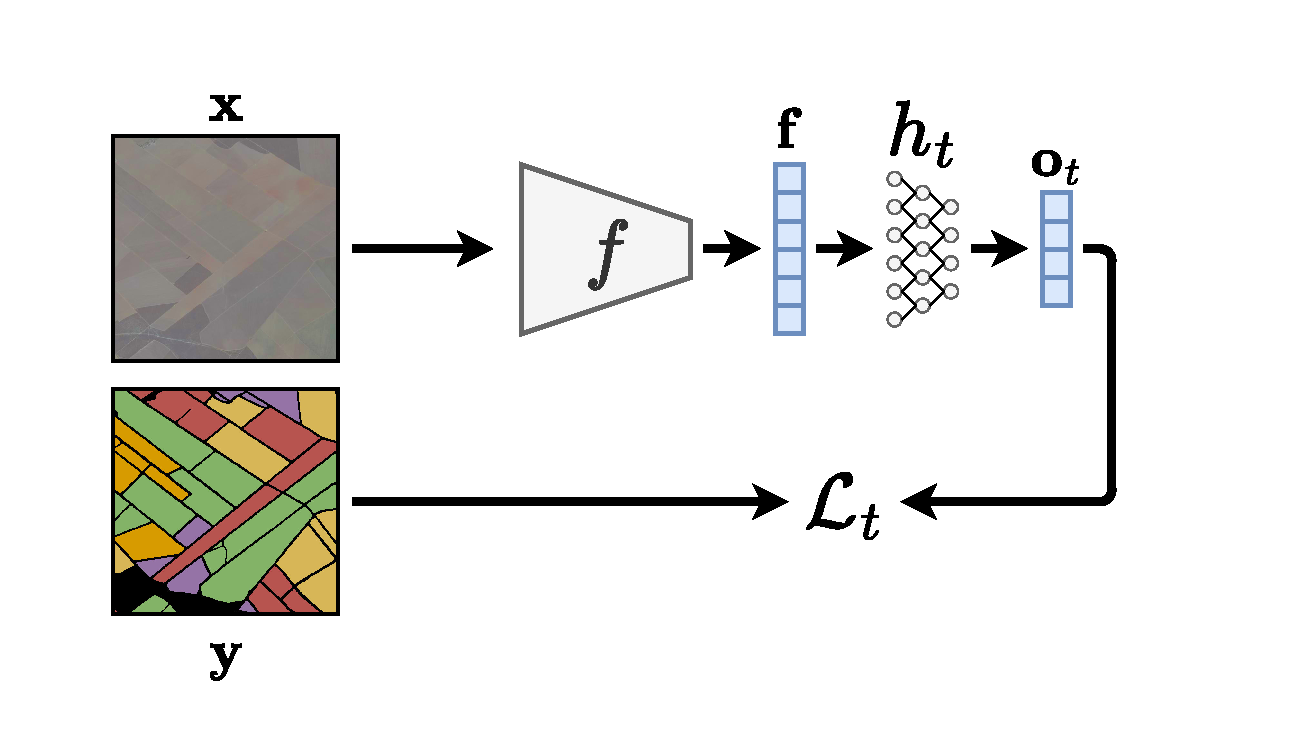
\includegraphics[clip,trim=0.75in 0.45in 0.45in 0.45in,scale=\figscale]{figures/3_theoretical_background/ssl/representation_learning_finetuning.pdf}
        \caption{\fromsurvey{}}
        \label{fig:ssl_overview_finetuning}
    \end{subfigure}
    \fignote{Overview of the self-supervised pretraining process (a) of a model $f$ using a loss $\mathcal{L}_p$ (a), followed by a fine-tuning step (b) to a target labeled task via a loss $\mathcal{L}_t$ (b). One should notice that only the backbone $f$ is maintained, while the pretraining head $h_p$ is swapped for a novel, randomly initialized target task head $h_t$.}
    \label{fig:ssl_overview}
\end{figure}

\fromsurvey{Visual \ac{SSL} began with transform prediction, i.e., procedurally augment an image using geometric, color, or masking transforms and train a model to predict which transform parameter was applied to that image. More formally, given an image $\mathbf{x}$, one can apply a randomly sampled transform $\tau \sim \mathcal{T}$ to generate the transformed version $\hat{\mathbf{x}}$. $\hat{\mathbf{x}}$ can then be passed forwarded through a backbone model $f$, yielding feature vector $\mathbf{f}$. The backbone $f$ and head $h$ are, therefore, trained to predict which randomly sampled transformation $\tau$ was applied to $\mathbf{x}$. For instance, classifying which rotation \citep{gidaris2018unsupervised} or affine transform \citep{kanazawa2016warpnet} a given image underwent. Some tasks not commonly used as data augmentations were also used, like jigsaws on the image, and the pretext task was to classify the correct order for the reconstruction of the original image \citep{kanazawa2016warpnet}. A prototypical transform prediction \ac{SSL} approach can be seen in Figure \ref{fig:ssl_transform}.}

\begin{figure}[ht!]
    \centering
    \caption{Overview of transform prediction self-supervised learning}
    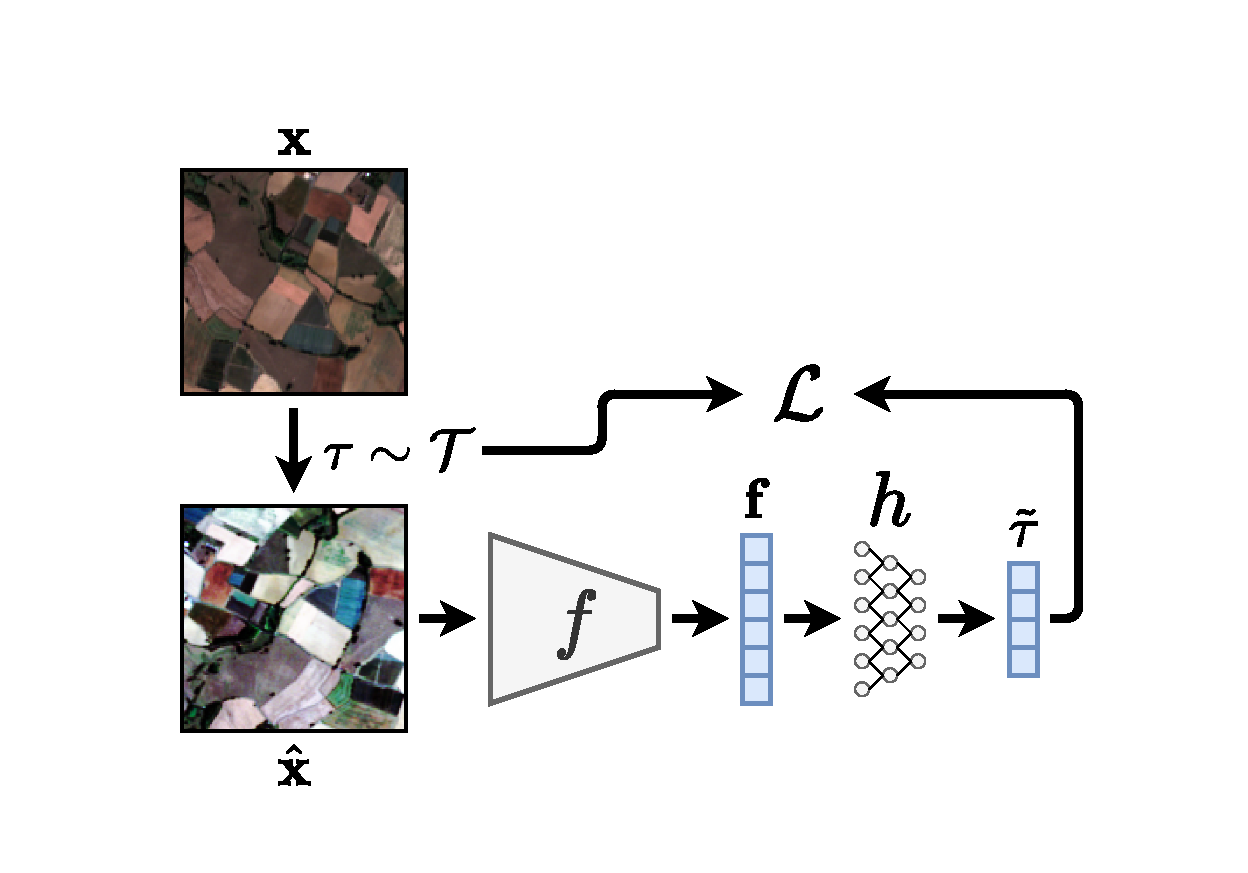
\includegraphics[clip,trim=0.75in 0.45in 0.45in 0.45in,scale=\figscale]{figures/3_theoretical_background/ssl/transform_prediction.pdf}
    \fignote{The original image $\mathbf{x}$ is transformed using $\tau \sim \mathcal{T}$ into $\hat{\mathbf{x}}$, which is fed through the networks $f$ and $h$ to predict $\tilde{\tau}$. A classification or regression loss $\mathcal{L}$ is then used to enforce that $\tilde{\tau} \approx \tau$.}
    \label{fig:ssl_transform}
\end{figure}

\fromsurvey{Little work has been done on transform prediction for \ac{RS}. \cite{wen2021rotation} used rotation prediction for object recognition using \ac{SAR} data, improving few-shot recognition performance. Again, \cite{xu2021self} employed the same methodology for object recognition for optical data. The latter also notes that doing this during semi-supervised hybrid training (see more in Section \ref{sec:ssl_semi}) presents slightly better results.}

\subsection{Similarity-based Self-Supervision}
\label{sec:ssl_similarity}

\fromsurvey{However, transform prediction \ac{SSL} has severe limitations, such as generating covariant embeddings with respect to the transformations applied to the input, as well as unrepresentative representations caused by the backbone learning to identify shortcuts instead of relevant features \citep{minderer2020automatic}. 
In order to extract more representative representations, \ac{SSL} has migrated to similarity-based techniques. Such methods approximate embeddings for multiple views of a single image, rendering the backbones invariant to these data augmentations instead of covariant to them. By doing this, the pretraining procedure encourages the representation to discriminate across instances, generating more sparse embeddings.}


\fromsurvey{Figure \ref{fig:ssl_sim} depicts a similarity-based \ac{SSL} strategy. From a single image $\mathbf{x}$, two views $\mathbf{x}_1 = \tau_1(\mathbf{x})$ and $\mathbf{x}_2 = \tau_2(\mathbf{x})$ are generated by applying two randomly sampled transformations $\tau_1, \tau_2 \sim \mathcal{T}$. $\mathbf{x}_1$ and $\mathbf{x}_2$ are then passed through a backbone $f$, yielding the feature representations $\mathbf{f}_1$ and $\mathbf{f}_2$, which are then passed through a projection head $h$, resulting in the projected vectors $\mathbf{p}_1$ and $\mathbf{p}_2$. The whole ensemble is then trained by encouraging similarity between $\mathbf{p}_1$ and $\mathbf{p}_2$ via a similarity loss $\mathcal{L}_{sim}$.}


\begin{figure}[ht!]
    \centering
    \caption{Overview of similarity self-supervised pretraining.}
    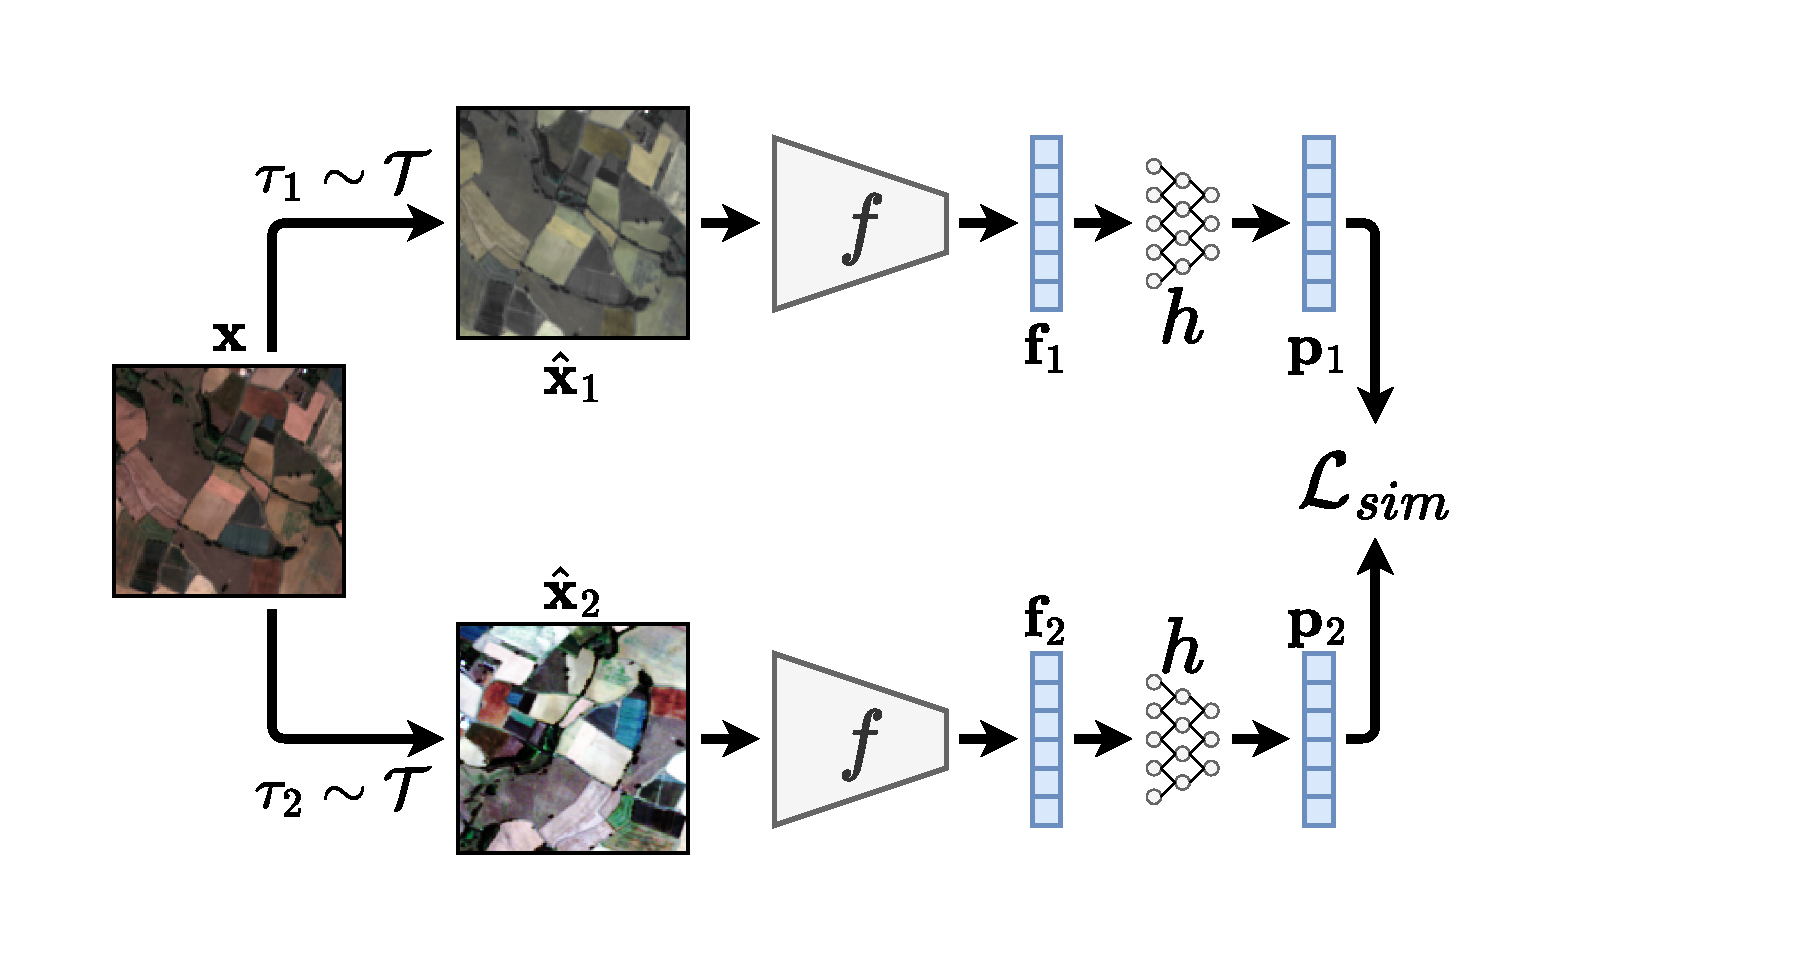
\includegraphics[clip,trim=0.75in 0.45in 2.4in 0.45in,scale=\figscale]{figures/3_theoretical_background/ssl/similarity.pdf}
    \fignote{ Two views $\mathbf{x}_1$ and $\mathbf{x}_2$ from a sample $\mathbf{x}$ computed using the transformations $\tau_1$ and $\tau_2$ are passed through a backbone $f$ and a projection head $h$, yielding projections $\mathbf{f}_1$ and $\mathbf{f}_2$, which are then encouraged to be similar via a similarity loss $\mathcal{L}_{sim}$.}
    \label{fig:ssl_sim}
\end{figure}

\subsubsection{Contrastive Self-Supervised Learning}
\label{sec:ssl_contrastive}

\fromsurvey{In order to avoid the mode collapse problem caused by enforcing similarity between different views of the same image (positive pairs), contrastive \ac{SSL} methods employ very large batch sizes to hold several negative pairs in each learning iteration. Thus, pretraining such contrastive methods may require several \acs{GPU}s with large \ac{VRAM} capacity. \ac{SimCLR} \citep{chen2020simple}, for instance, is a highly influential contrastive \ac{SSL} strategy that requires very large batch sizes. In this approach, the normalized temperature-scaled cross-entropy loss (NT-Xent) is used, leveraging negative pairs from other samples in the batch and achieving a top-1 \ac{OA} of 79.8\% in ImageNet.}

\fromsurvey{Multiple strategies employ smarter ways to leverage negative pairs to avoid the need for large batch sizes. \Acf{MoCo} \citep{he2020momentum, chen2020improved, chen2021empirical} uses a dictionary implemented with a Round Robin queue that stores previously batched negative samples. This makes it possible to decouple the problem of the number of negative pairs from the batch size. In \ac{MoCo}, the key encoder is updated smoothly using a moving average of the query encoder (momentum). This approach leverages the InfoNCE loss to minimize the distance between a query and its positive key and maximize the distance to negative keys, resulting in 81\% in ImageNet in its more recent version.}

\fromsurvey{Another approach to addressing large batch sizes was taken by \cite{caron2020unsupervised} propose \Acf{SwAV} as a pretraining \ac{SSL} strategy. \ac{SwAV} works by predicting online clusters for each augmented multiresolution view of the images via the Sinkhorn-Knopp algorithm. The method does not use direct comparisons between embeddings generated by the augmentations, which eliminates the need for large batch sizes. Instead of traditional instance-wise contrastive learning, \ac{SwAV} is understood as a contrastive clustering approach. As a result, \ac{SwAV} achieved 75.3\% in the same test procedure as \ac{SimCLR} and \ac{MoCo}. \ac{SwAV} was the first \ac{SSL} method to overcome supervised pretraining in ImageNet in transfer learning tasks to other downstream RGB datasets.}

\fromsurvey{Barlow Twins \citep{zbontar2021barlow} use negative samples from the batch itself without the need for a large batch size. This is achieved via a more thorough grid search on the optimizer's hyperparameters. Using a Siamese network that processes two augmented views of the data, Barlow Twins generates a cross-correlation matrix of the augmented embeddings -- twins -- of the batch and trains the network to approximate the identity matrix. By approximating the values of the main diagonal to 1, it forces the invariance of the augmentations. By approximating the other values of the matrix to 0, it avoids collapse. The method has performance comparable to previous methods, including some non-contrastive methods (see Section \ref{sec:ssl_non_contrastive}).}

\fromsurvey{\Acf{SeCo} \citep{yao2021seco} specifically addresses video tasks such as action recognition, untrimmed activity recognition, and object tracking. For this, the models are pretrained on videos, and three pretrained tasks were designed for this: intra-frame discrimination, which determines whether two image patches belong to the same video frame, inter-frame discrimination, which determines whether two image patches belong to the same video, and temporal order validation, which checks whether a sequence of patches is in the correct temporal order. This leads to an improvement in action recognition \ac{OA} of 2.96\% and 6.47\% on UCF101 and HMDB51 against supervised ImageNet pretraining.}

\fromsurvey{Traditional contrastive \ac{SSL} has been employed in RS tasks. \cite{ayush2021geography} adapted \ac{MoCo} by adjusting its augmentations that originally were designed for natural images. For this, temporal views of the same image are used as positive pairs, while images from different positions are used as negative samples. In addition, the prediction of the geolocation of the region of interest is incorporated into the pretext task. For this, the coordinates of the images are previously clustered using K-Means, and the prediction of which cluster each image belongs to is added to the loss. Results indicate that the method outperforms \ac{MoCo} in \ac{RS} tasks. \Acf{DeCUR} \citep{wang2024decoupling} follows the Barlow Twins paradigm, separating inter-modal representations (shared across data modalities) and intra-modal representations (unique within each data modality), enabling the model to learn both shared characteristics and modality-specific features. \ac{DeCUR} outperforms multiple \ac{SSL} methods designed for natural images in both classification and semantic segmentation of images. \ac{SeCo} \citep{yao2021seco} was also used in \ac{RS} \citep{Manas_2021_ICCV} settings, in this case with very few modifications. The results obtained were better in several downstream tasks compared to \ac{MoCo}. These results reinforce the need for domain-specific augmentations in visual \ac{SSL}.}

\subsubsection{Non-Contrastive Self-Supervised Learning}
\label{sec:ssl_non_contrastive}

\fromsurvey{More recently, techniques that do not depend on negative samples have emerged, which completely get rid of the need for memory to store them, either in large batches or in other structures. \Acf{BYOL} \citep{grill2020bootstrap} showed that negative pairs are not needed for avoiding mode collapse. \ac{BYOL} employs two networks: \textit{online} and \textit{target}; wherein the \textit{online} network is trained in a traditional fashion and the \textit{target} is updated with an exponential moving average. The \textit{target} network incorporates a prediction head that projects the embeddings to avoid the collapse of the representations, getting 79.6\% on the same test of \ac{SimCLR}, but using a ResNet with 200 layers. \Acf{DINO} \citep{caron2021emerging} was heavily inspired by \ac{BYOL}, transforming it into a complete knowledge distillation architecture. \ac{BYOL} is heavily focused on optimizing convolutional networks such as ResNet, while \ac{DINO} shows that \acs{ViT}s, show interesting emergent properties of their pretraining. \acs{ViT}s pretrained with \ac{DINO} have internal activations more present in the most informative pixels in the images representing the classes, even with pretraining without labels, achieving 77\% in ImageNet with \acs{ViT}-B/8.}

\fromsurvey{\Acf{SimSiam} \citep{chen2021exploring} considerably simplified non-contrastive \ac{SSL} by approximating embeddings through a Siamese architecture, with one of the branches having an \ac{MLP} as a predictor, and the other applying a stop-gradient operation. The authors describe the method in several ways, including a \ac{SwAV} without online clustering and a \ac{BYOL} without an exponential moving average of the weights, achieving performance very close to contrastive methods. Compared to other non-contrastive methods, \ac{SimSiam} is minimalist, only including what really makes similarity-based \ac{SSL} work without negative pairs. \cite{pototzky2022fastsiam} further improved \ac{SimSiam} into \ac{FastSiam} by regularizing the pretraining by using multiple views instead of only two, achieving similar results, but with only a single \ac{GPU} used during training and a very small batch size.}

\fromsurvey{\cite{bardes2021vicreg} addressed mode collapse in another way, using two forms of regularization in the embeddings: a term that maintains the variance of each embedding dimension above a threshold and a term that decorrelates each pair of variables, creating the \Acf{VICReg} method. \ac{VICReg} does not use negative pairs, while also not using stop-gradient operations, achieving performances comparable to contrastive methods. \Acf{VICRegL} \citep{bardes2022vicregl} builds upon VICReg by adding a new branch to the network responsible for processing local visual information. Even though \ac{VICRegL} results in a 1.1\% drop in classification \ac{OA} in ImageNet, this strategy is shown to be more suited to semantic segmentation and detection tasks. VICRegL yields an 8.1\% mIoU improvement in Pascal VOC, showing that targeted \ac{SSL} pretraining can be better suited to downstream tasks other than image classification.}

\subsection{Masked Modeling}
\label{sec:ssl_mim}

\fromsurvey{Another group of widely used methodologies that draws inspiration directly from \ac{NLP} is \Acf{MM}, in which a portion of the input data for each sample is masked and the pretext task becomes reconstructing the original input data. A typical \ac{MM} approach can be seen in Figure \ref{fig:ssl_mim}. The original image $\mathbf{x}$ is initially sliced into patches, forming the patched image $\mathbf{w}$. A percentage of the patches is masked (hidden), forming $\hat{\mathbf{w}}$, while the masked pixels form the image comprising the invalid pixels $\mathbf{w}_i$. The valid patches are linearized, forming $\hat{\mathbf{w}}_v$ which is passed through the ViT backbone $f$ that serves as an encoder, resulting in the encoded representations $\mathbf{e}_v$. The masked patches are appended to $\mathbf{e}_v$, resulting in $\mathbf{e}_w$, which is passed through the decoder $g$. The output of the ensemble of networks is $\mathbf{d}_w$ representing an embedding with information about the reconstruction of the valid and invalid patches. From $\mathbf{d}_w$, only the originally masked patches are reconstructed in image $\tilde{\mathbf{w}}_i$, which is compared to $\mathbf{w}_i$ via a reconstruction loss $\mathcal{L}_{rec}$.}

\begin{figure}[ht!]
    \centering
    \caption{Overview of masked image self-supervised pretraining.}
    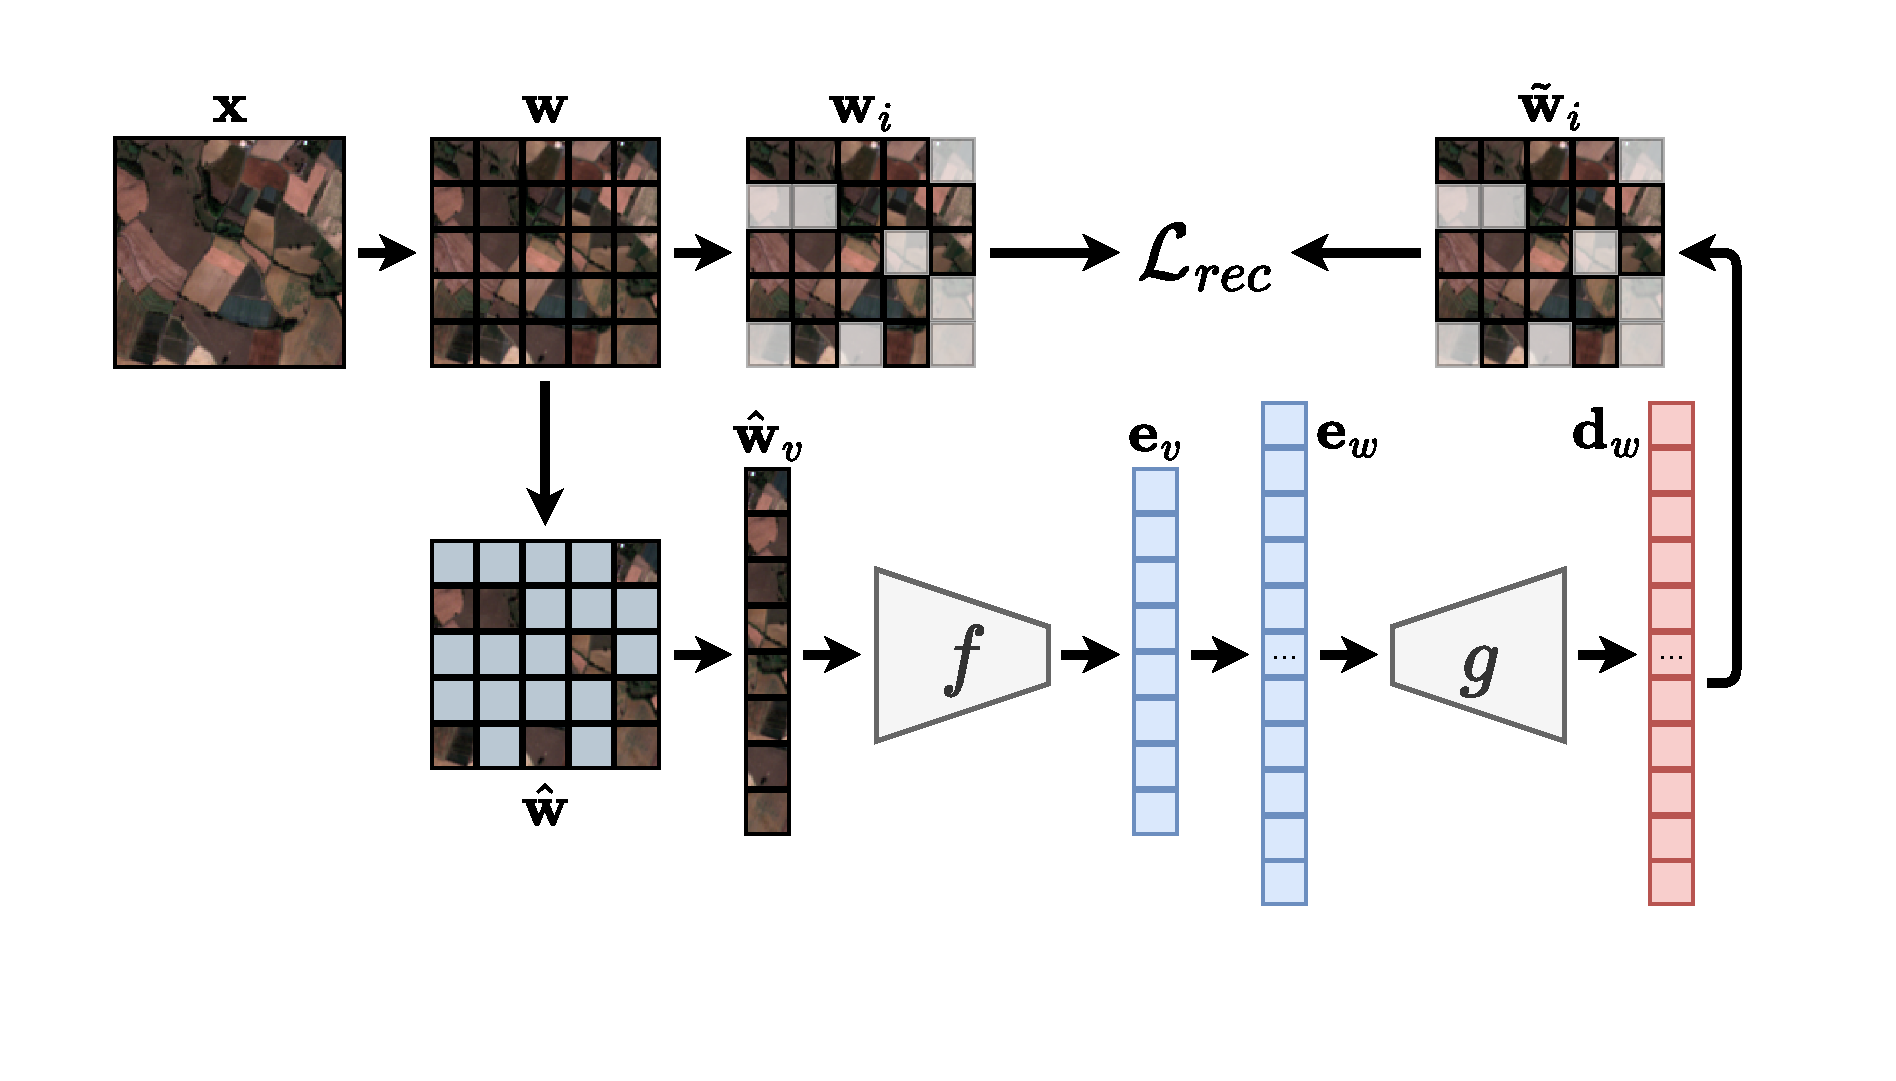
\includegraphics[clip,trim=0.55in 0.4in 0.95in 0.45in,scale=\figscale]{figures/3_theoretical_background/ssl/masked_image_modeling.pdf}
    \fignote{Initially, image $\mathbf{x}$ is windowed, forming $\mathbf{w}$, which yields the valid patch list $\hat{\mathbf{w}}_v$. The patches in $\hat{\mathbf{w}}_v$ are then passed through encoder $f$, resulting in the encoded vector $\mathbf{e}_v$, appended to reinsert the representations of the invalid (masked) patches, resulting in $\mathbf{e}_w$. $\mathbf{e}_w$ is then passed through the decoder $g$, resulting in the reconstruction embedding $\mathbf{d}_w$. From $\mathbf{d}_w$, the reconstruction of the masked patches $\tilde{\mathbf{w}}_i$ is compared to $\mathbf{w}_i$ via a loss $\mathcal{L}_{rec}$. Afterwards, $f$ is repurposed for fine-tuning to a downstream task.}
    \label{fig:ssl_mim}
\end{figure}

\fromsurvey{Following the \ac{MM} paradigm, \Acf{MAE} \citep{he2021maskedautoencodersscalablevision} masks patches from a ViT. The authors showed that the best strategy is to pretrain with 75\% of the patches randomly masked, achieving 76.6\% in ImageNet with a ViT-H/14. Furthermore, it was shown that reconstructing an image without masking patches results in ineffective pretraining, since it is not a complex enough task to force the networks to learn representative features. \Acf{SimMIM} \citep{xie2022simmim} is an approach that works as an advancement and simplification of \ac{MAE}, using direct regression of the RGB values of masked pixels and a lightweight linear decoder head, rendering it a highly efficient pretraining strategy.}

\fromsurvey{Generalist approaches for RS using the idea of data masking have also been developed. \cite{reed2023scale} adapted \ac{MAE} for this domain, introducing a positional encoding based on the spatial resolution of the images. In addition, their Scale-\ac{MAE} separately reconstructs low and high-frequency components using a Laplacian decoder, allowing multiscale learning, while the classic \ac{MAE} reconstructs only the original image. This makes Scale-\ac{MAE} more robust for remote sensing by dealing with multiple scales. The authors demonstrate the improvement in several downstream tasks, including also demonstrating embedding improvement via K-Nearest Neighbors analysis. \cite{xiong2024neural} extended the method based on the idea of neuroplasticity, being able to deal with any number of spectral bands and sensor modalities. Their approach uses a hyper-network-based dynamic weight generator that adjusts its architecture for new sensors, having as input the central reflectance value of each of the bands in addition to the images.}

\fromsurvey{More recent work uses a method that combines MIM with Similarity-based \ac{SSL}, in which views are approximated, but with some having patches of their data masked. Masked Siamese Network (MSN) \citep{assran2022masked} approximates two views of the same image through Negative Cosine Similarity. In the anchor view, some data is masked, while the target view undergoes more aggressive color and geometric augmentations, aiming to render the model invariant to them. Prior Matching for Siamese Networks (PMSN) \citep{assran2022hidden} demonstrated that, although the previous methods do not require pretraining labels, it is still assumed that the classes that exist in the datasets are approximately balanced. To address this, the authors modified the loss function to include a power-law in order to force a balancing of classes per batch, improving the performance on imbalanced data, but degrading the performance on balanced datasets.}

\begin{figure}[ht!]
    \centering
    \caption{\fromsurvey{Overview of masked image similarity self-supervised pretraining.}}
    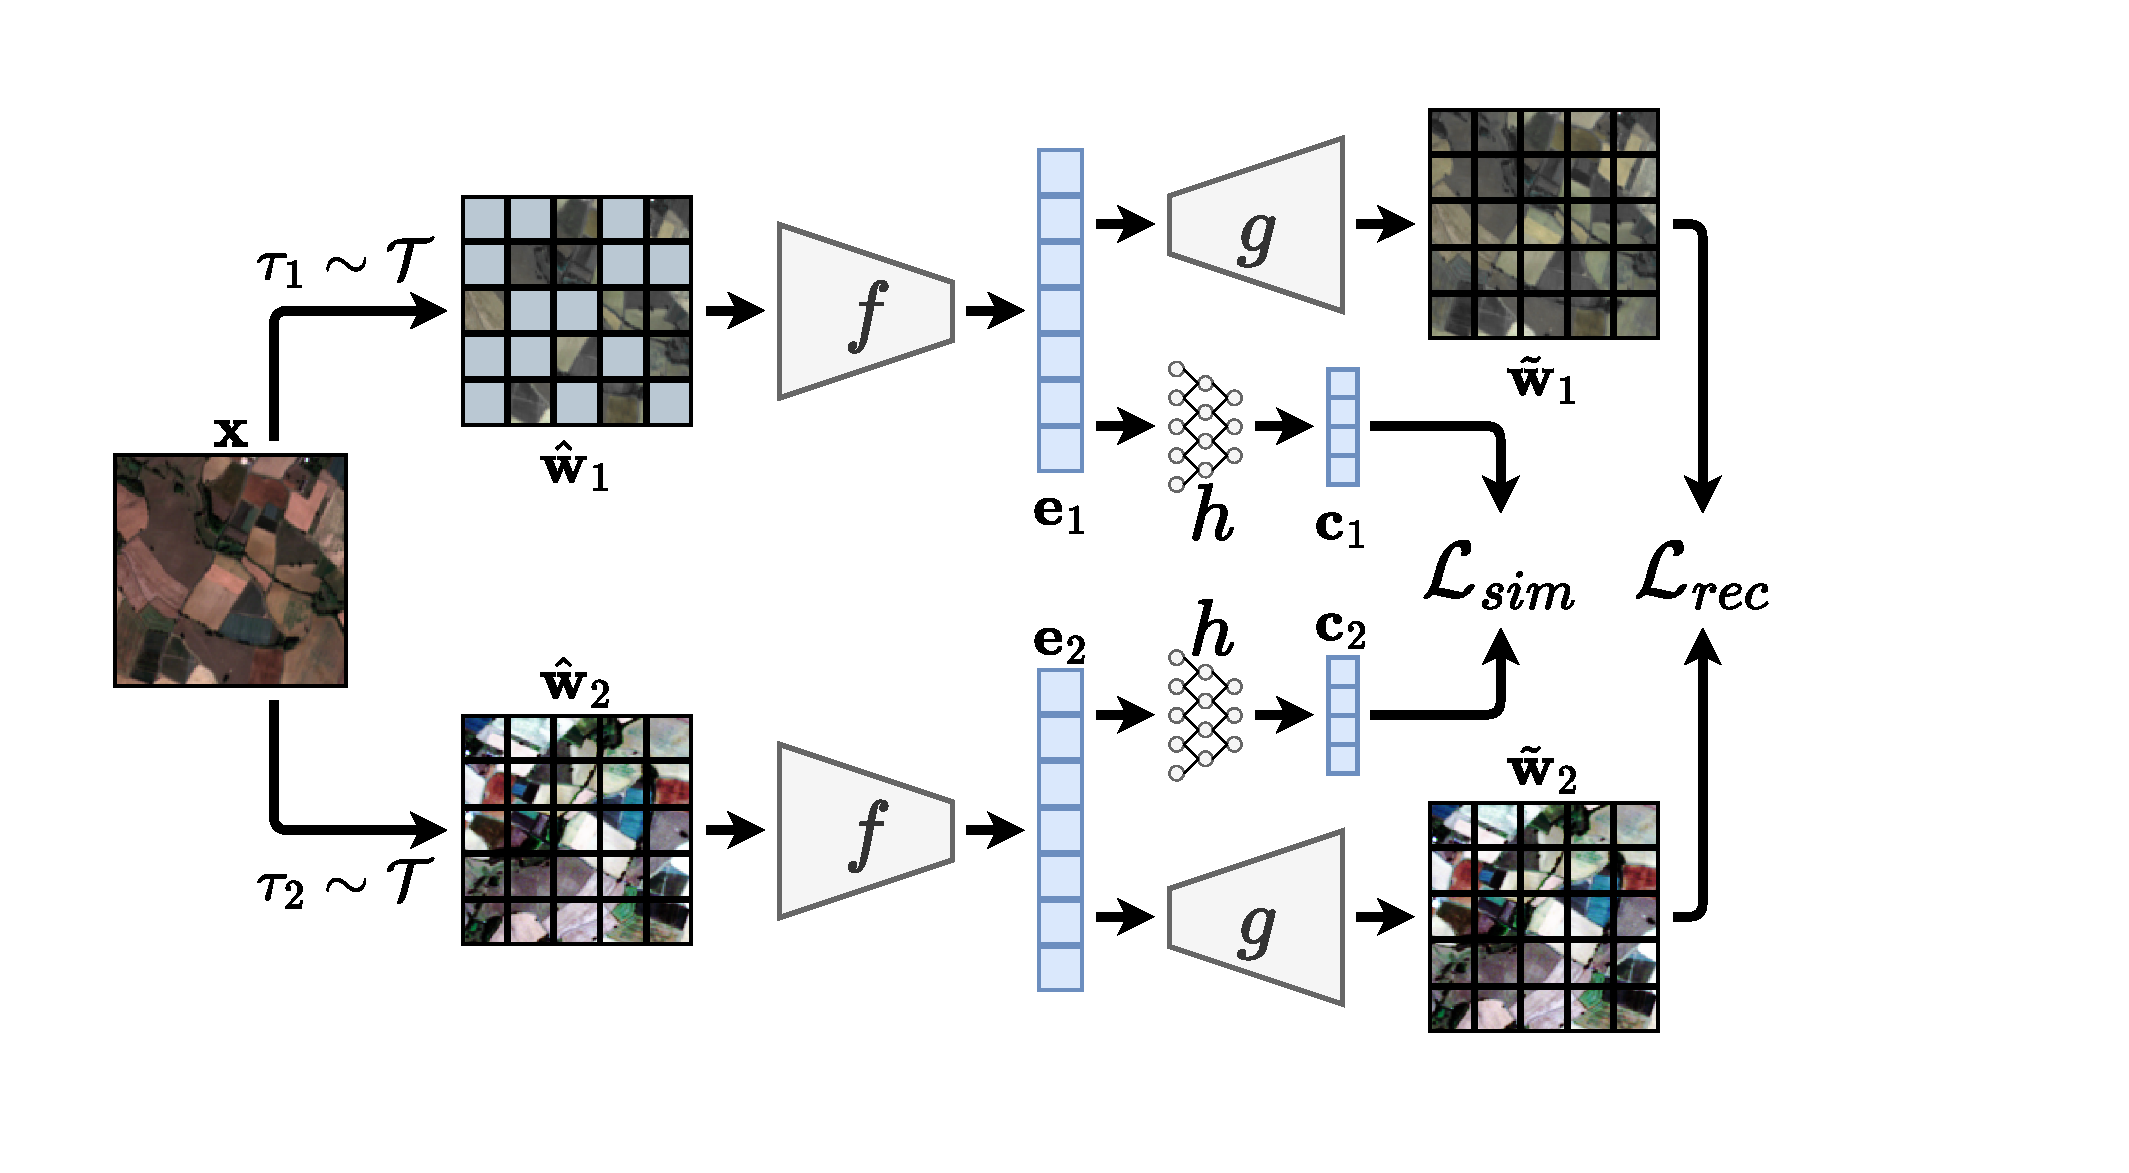
\includegraphics[clip,trim=0.75in 0.45in 2.2in 0.45in,scale=\figscale]{figures/3_theoretical_background/ssl/masked_image_modeling_similarity.pdf}
    \label{fig:ssl_mim_sim}
\end{figure}

\subsection{Semi-Supervised Hybrid Techniques} \label{sec:ssl_semi}

\fromsurvey{A very small area with few published works seeks to combine characteristics of semi-supervised learning with self-supervised learning, based on the hypothesis that \ac{SSL} can benefit from a small number of labeled samples. For this, strategies are used in which the \ac{SSL} pretext task on unlabeled data is performed during finetuning for the downstream task, in a semi-supervised fashion. Following this strategy, \cite{zhai2019s4l} then proposed the \Acf{S4L} method that classifies two augmentations of an image labeled with CELoss, and predicts transforms for these two augmentations added to two more from the unlabeled dataset, achieving the best performance in \ac{OA} on the ILSVRC-2012 Dataset, although comparisons with other methods are lacking. Few methods in this family have been used in \ac{RS}. \cite{singh2018self} used rotation prediction to aid classification, combining the two losses into a so-called Mixup Loss. The results were slightly better using this method, especially considering that rotation prediction in satellite images is quite complex since the directions in the images do not contain much semantic meaning.}
\section{Confidence Estimation and Anomaly Rebuttal}
\label{sec:conf_contextualization}

The use of \ac{DL} models in critical applications - such as autonomous driving, medical diagnosis, and, in the context of this work, large-scale agricultural monitoring - makes the reliability of these models a primary concern. It is not enough to simply search for models with high evaluation metrics; it is essential that such models be capable of assessing the reliability of their own predictions and identifying when a prediction is subject to significant uncertainty.

Historically, the standard approach to estimating the confidence of a classification model has been to use Maximum Class Probability (MCP), obtained directly from the softmax layer of the network, which is usually the last layer of a classification Deep Neural Network. However, the literature points out that MCP has significant conceptual flaws for confidence prediction. The main problem lies in the fact that modern neural networks are overconfident~\citep{NEURIPS2021_61f3a6db,pmlr-v162-wei22d}, assigning high probabilities even to incorrect predictions. This results in considerable overlap in the confidence distributions between hits and misses, making the raw use of network outputs poor confidence rankings.

\cite{corbiere2019addressing} proposes ConfidNet, an auxiliary neural network that estimates the reliability of a classification model's predictions, proposing the use of True Class Probability (TCP) as a target metric to distinguish failures, since the output of the last layer tends to be overconfident, even in incorrect predictions. In terms of methodology, ConfidNet is trained on the feature extraction layers of an already trained classifier, whose weights are kept frozen during the initial phase. Subsequently, the backbone of the original classifier is copied and its weights are fine-tuned together with the auxiliary confidence prediction network. The network minimizes an MSE calculated between the confidence predicted by ConfidNet and the probability that the original classifier assigned to the ground truth of that specific sample. As for the network architecture itself, it consists of linear layers with ReLU activation, ending with a sigmoid activation to ensure that the output is in the range of 0 and 1. This technique can be applied to any classifier network and will therefore be used as a baseline in this work.

While traditional classification assumes a closed set scenario, where all possible classes are known during training, the \acf{OSR} scenario, i.e., open set, assumes that the model must correctly classify known classes while identifying samples belonging to unknown classes~\citep{10582552}. \ac{OSR} techniques can be adapted to the confidence problem by treating incorrect predictions as anomalies or outliers in the model's embedding space. In this context, \acf{GeMOS}~\citep{vendramini2021opening} proposes a plug-and-play framework that couples a \ac{GMM} per predicted class on the embeddings of the network's intermediate layers extracted by a supervised \ac{CNN} trained on a closed set, with the training of the \ac{GMM}s limited to the training samples for which the network made correct predictions. During inference, the model calculates a likelihood score that indicates how well a sample fits the distribution of the predicted class, where low likelihood values suggest that the sample is an anomaly (or a classification error). Similarly, \cite{10418501} also suggests using \ac{GMM}s to model the distribution of embeddings, but using superpixels for \ac{OSR} in semantic segmentation.

\begin{figure}[ht!]
\centering
\caption{Comparison between closed set and open set classification.}
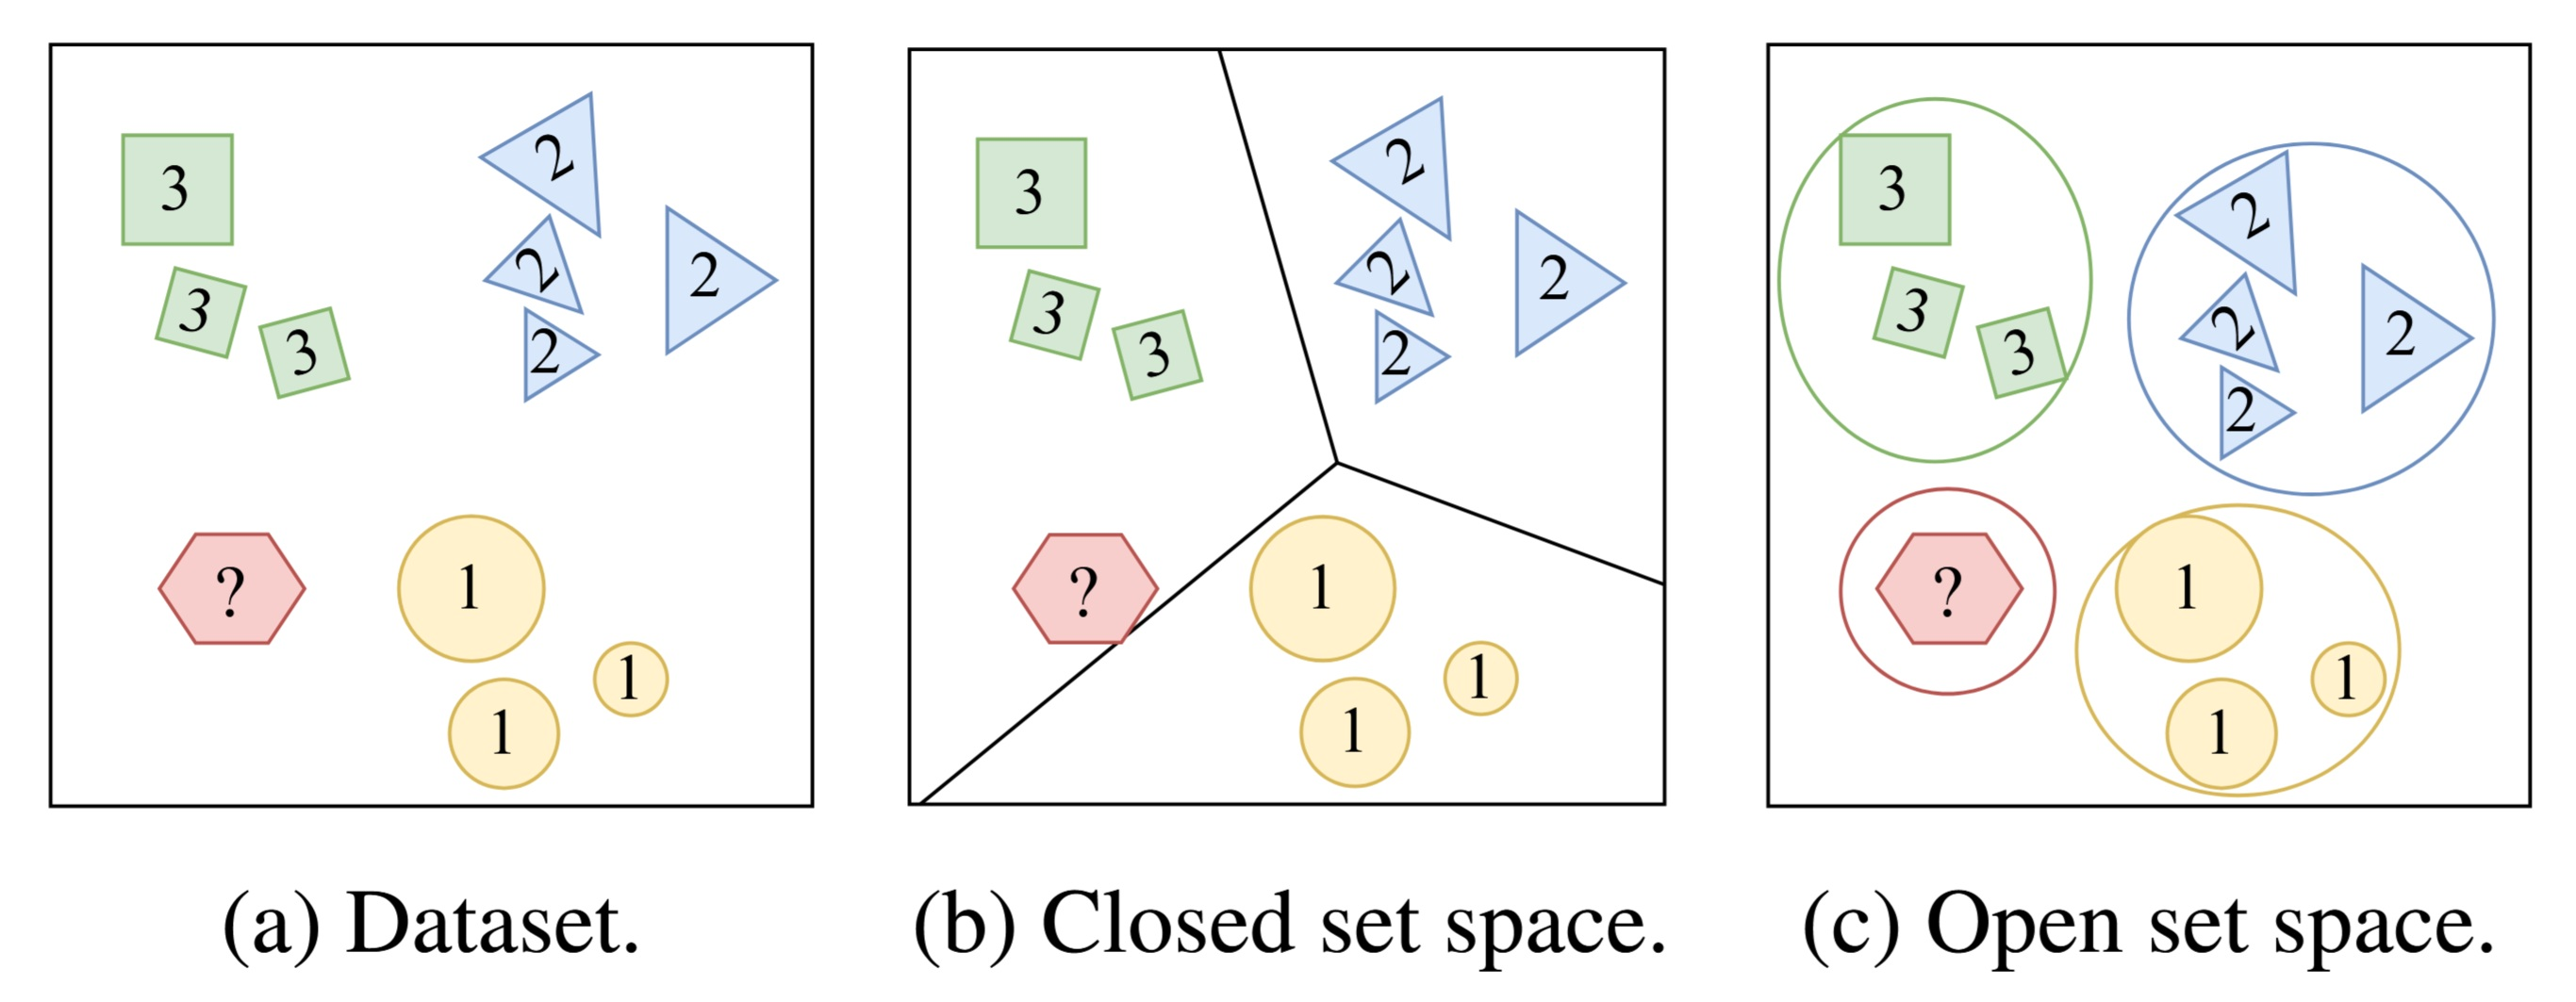
\includegraphics[width=0.95\linewidth]{figures/3_theoretical_background/gemos.jpg}
\fignote{One should notice that, in Closed Set (b) the sample ``?'', from a new class, would be classified erroneously as class 3. In Open set (c), the sample would be classified as an ``unknown'' class - Adapted from \cite{vendramini2021opening}}
\label{fig:osr}
\end{figure}

In addition to generative models on embeddings, other techniques seek semantic consistency by reconstructing the input data. The Conditional Reconstruction for Open-set Semantic Segmentation (CoReSeg) method~\citep{9897407} uses a conditional reconstruction approach, where the network attempts to reconstruct the input image only on known classes, which are those present in the training dataset. The premise is that objects of known classes will be well reconstructed, while unknown objects or classification errors will result in a high reconstruction error.
\chapter{Related Works}\label{chapter:related_works}

This chapter presents a literature review focusing especially on work with public mission sensors, and is organized as follows: section \autoref{sec:rreview} presents previous surveys and reviews relevant to the work. Section \ref{sec:taxonomy} proposes a taxonomy to categorize applications in the area, and the following sections detail such applications, such as Parcel Delineation (\autoref{sec:parcel_segmentation}), Crop Mapping (\autoref{sec:crop_mapping}), Crop Yielding (\autoref{sec:crop_yielding}), LULC (\autoref{sec:lulc}), and Change Detection (\autoref{sec:change_detection}). Finally, \autoref{sec:rdiscussion} presents a critical discussion of the state of the art, identifying gaps in the literature.

\section{Reviews}\label{sec:rreview}

Some systematic reviews have been conducted covering aspects of agricultural \ac{RS} using machine learning. \fromsurvey{As an example, the work conducted by \cite{yuan2020deep} serves as introductory material for the use of \ac{DL} focusing on environmental applications. In contrast, \cite{ma2019deep} cover both urban and agricultural \ac{RS}, though their focus is on urban applications. The most referenced application is \ac{LULC}, with almost twice as many papers as second place, Object Detection. Data Fusion only appears in fifth place. As the most common architecture, \acs{CNN}s are the architecture of choice in this domain, being five times more used than \ac{AE}. The use and good results with \ac{HR} and \ac{VHR} images continued. However, there are a few multi-temporal methodologies cited that are useful in agriculture.  Also, due to its release date, this review does not cover the current rapid growth of attention-based architectures in agricultural \ac{RS} applications, including Transformers and Data Fusion applications.}

\fromsurvey{Another review was conducted by \cite{li2022deep} that studied multimodal Data Fusion in \ac{RS} considering 598 papers, from 2015 to 2022, focusing on tasks like classification (i.e. segmentation), cloud removal, and object detection. The research incorporated multiple data types such as medium and high-resolution imagery, \ac{LiDAR}, and \ac{SAR} data. They identified \acs{CNN}s as the predominant models. Despite a notable rise in publications about this subject, the authors highlighted a deficiency of datasets specifically for agricultural uses in their study. Additionally, they mentioned an issue with the interpretability and validity of synthetic data produced through Data Fusion.}

\fromsurvey{\cite{aleissaee2023transformers} mapped the use of \acs{ViT}s in \ac{RS} using 60 papers. Primarily, high-resolution multispectral imagery was used, sometimes in combination with \ac{SAR} data. The majority of papers cited in this work refer to either classification or detection problems. The survey also noted that pretraining using \ac{RS} data instead of natural images - in most cases, ImageNet Dataset \citep{deng2009imagenet} - tends to provide better outcomes. Nevertheless, this survey did not include unsupervised pretraining, i.e., \ac{SSL}; the authors noted the absence of large-scale datasets for unsupervised pretraining. Additionally, techniques applied to \ac{SITS} were not charted in this study.}

\fromsurvey{As noted in previous efforts \citep{liu2024diffusion}, following the trend of traditional computer vision literature, \ac{RS} researchers have started to adopt diffusion models, especially since 2023. In addition, the authors argue that satellite imagery presents some noise: optical imagery presents atmospheric dispersion of \ac{EMR}, which is usually improved by so-called atmospheric corrections models \citep{li2018amosphericcorrection}; on the other hand, \ac{SAR} data has speckle inherent due to the out-of-phase reflection of \ac{EMR} from the target \citep{dasari2015sarspeckle}.For this reason, diffusion models tend to perform well because they learn latent representations that are robust to noise due to diffusion. Although the first applications were for data synthesis (i.e., Super Resolution and Cloud Removal), there are already applications for image interpretation. The authors did not specifically address agricultural applications.}

\fromsurvey{When it comes to applications, \cite{joshi2023remote} reviewed Crop Mapping and Yield in 81 selected papers. Unlike the abovementioned surveys, the authors stated that low and medium resolution optical imagery was most frequently used. Sentinel-1 MSI/Sentinel-2 data are usually used for crop mapping, while the most commonly used satellite for crop yield is \ac{MODIS}. As for \ac{DL} architectures, the most widely used model is \ac{CNN}, with more than twice the number of uses of second place, \ac{RNN}. U-Net stands out in \ac{CNN}, especially U-Net 3D for considering time series. Moreover, attention mechanisms are frequently incorporated into these architectural frameworks. Concerning the challenges identified, the authors noted a deficiency of datasets, which hinders the development of models capable of generalizing effectively. Furthermore, there is a lack of research dedicated to the interpretability of predictions.}

\fromsurvey{Both \cite{weiss2020remote} and \cite{joshi2023remote} present more recent reviews of the \ac{RS} literature, though with little information on automating image understanding using \ac{DL} and ML in general. Multiple studies indicate that crop mapping with optical data combined with \ac{SAR} leads to better results. For crop yielding, combining satellite data with \textit{in-situ} data, soil, and climate information is often an effective approach.}

\fromsurvey{Most recently, \cite{kamilaris2018deep} published the latest survey on \ac{DL} in agricultural \ac{RS}, in 2018. Authors noted that the use of \ac{DL} for \ac{RS} can generate better outcomes, hence being an alternative for shallow learning. The authors pointed out that, even today, there is a limited number of publicly available agricultural \ac{RS} datasets. Nonetheless, due to its publication date, methodologies such as \ac{SSL} were not presented in this survey.}

\fromsurvey{Also, in a more specific direction, \cite{sishodia2020applications}, reviewed the main Precision Farming methods. The survey highlighted the importance of this \ac{RS} technique for increasing agricultural productivity while minimizing environmental and social impacts. However, the review does not provide much information regarding \ac{DL} though it emphasized the method was likely to become increasingly important in meeting this challenge.}

\fromsurvey{\cite{9875399} made an extensive survey of Self-Supervised Learning methods applied to the context of urban and agricultural \ac{RS} in 2022. Traditional methods that utilize red, green, and blue (RGB) images inspired techniques for analyzing multi- and hyperspectral satellite images; similar approaches for time series were also influenced by these methods. In contrast, there are no experimental analyses for agricultural datasets. The only application tested in this work was \ac{LULC}, which is shown to be less effective for agricultural studies compared to other applications. In addition, due to its publication date, only studies up to 2021 were analyzed, and, as shown in Section \ref{sec:taxonomy}, the area has advanced significantly using modern techniques better adapted to \ac{RS} and agricultural \ac{RS}.}

\fromsurvey{\cite{begue2018remote} presented a similar review, focusing on \ac{RS} for mapping cropping practices. The authors categorize applications into crop succession, cropping patterns, and crop management techniques. However, the survey uses data from both public and commercial missions. Furthermore, due to the publication date, the survey does not include techniques such as attention models and \ac{SSL}.}

\fromsurvey{Finally, \cite{weiss2020remote} present a meta-review of the main surveys in the area of \ac{RS} for agriculture. Their study considered research up to 2019, although they did not mention the number of studied reviews. The study also includes the use of machine learning techniques on satellite data, as well as on \ac{UAV} and \ac{LiDAR}, despite not presenting a direct comparison between their results. The paper provides a summary of the typical data types employed in various applications.}

\section{Taxonomy}
\label{sec:taxonomy}

Regarding our fine-grained review, we researched papers for all useful applications in an agricultural monitoring pipeline using \ac{RS}, with a greater focus on \ac{DL} and Self-Supervised Learning. It should be noted that some papers outside the query were added due to their importance to the field. \fromsurvey{We found 905 articles on this topic, 2 of which were published under the same name in different journals. Most are from Scopus, ACM, IEEE and arXiv journals, using the FindPapers algorithm \citep{grosman2020findpapers}, considering papers from $1^{st}$ January 2019 to $2^{nd}$ December 2024. We emphasize that we only selected papers that use optical and radar images from satellites. \ac{UAV} and \ac{LiDAR} sensors on board UAVs or satellites were not considered, as there are differences in spatial resolution and data processing, which would lead to difficulties in comparing the different techniques.}

\fromsurvey{The query used for selecting papers is as follows:}

\begin{quote}
	Query = ``([\textsc{deep learning}] OR [\textsc{DL}] OR [\textsc{self-supervised}] OR [\textsc{self-supervised learning}] OR [\textsc{SSL}] OR [\textsc{MoCo}] OR [\textsc{SeCo}] OR [\textsc{SimSiam}] OR [\textsc{VicregL}] OR [\textsc{DINO}] OR [\textsc{BYOL}] OR [\textsc{Masked Auto Encoder}] OR [\textsc{SWaV}] OR [\textsc{SimCLR}]) AND ([\textsc{crop}] OR [\textsc{land cover}] OR [\textsc{change detection}] OR [\textsc{deforestation}] OR [\textsc{agriculture}]) ND NOT ([\textsc{survey}] OR [\textsc{review}]) AND NOT ([\textsc{urban}]) AND ([\textsc{remote sensing}]) AND NOT ([\textsc{lidar}] OR [\textsc{uav}])''
\end{quote}

\fromsurvey{To visualize our results, we show in Figure \ref{fig:tax_publishedpapers} a diagram of publications per publisher, which shows that the vast majority of publications in this area were published by Scopus, followed by IEEE. In addition, the number of publications per year is shown in Figure \ref{fig:tax_papersperyear}. The increase in published papers between 2023 and 2024 is evident and can be attributed to several factors, one of which is the accessibility of cloud computing. In addition, we have conducted an analysis of the frequency with which these approaches have been used over time (see Figure \ref{fig:tax_approaches_years}).}

\begin{figure}[htbp]
	\centering
	\caption{\fromsurvey{Diagram for papers and their publishers.}}
	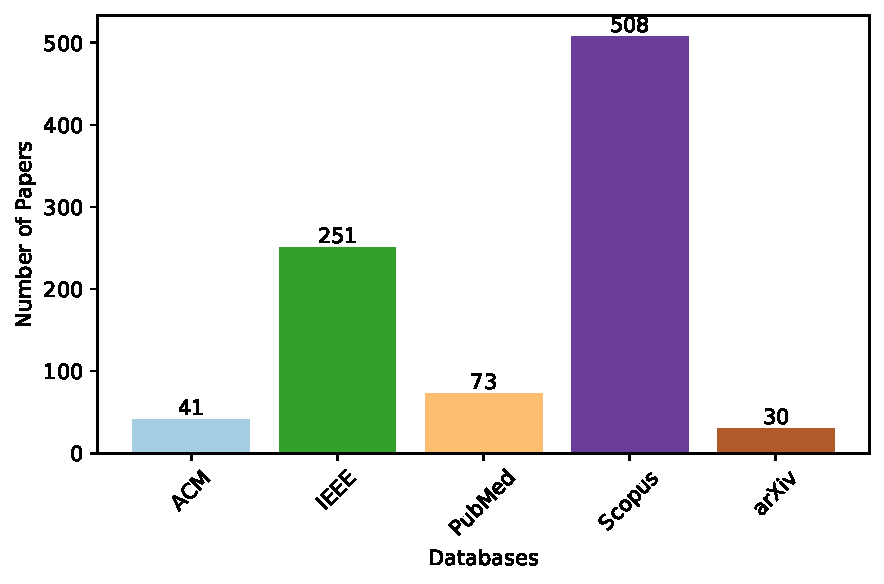
\includegraphics[width=.85\linewidth]{figures/4_related_works/taxonomy/count_published_papers.pdf}
	\label{fig:tax_publishedpapers}
\end{figure}


\begin{figure}[htbp]
	\centering
	\caption{\fromsurvey{Number of published papers per year.}}
	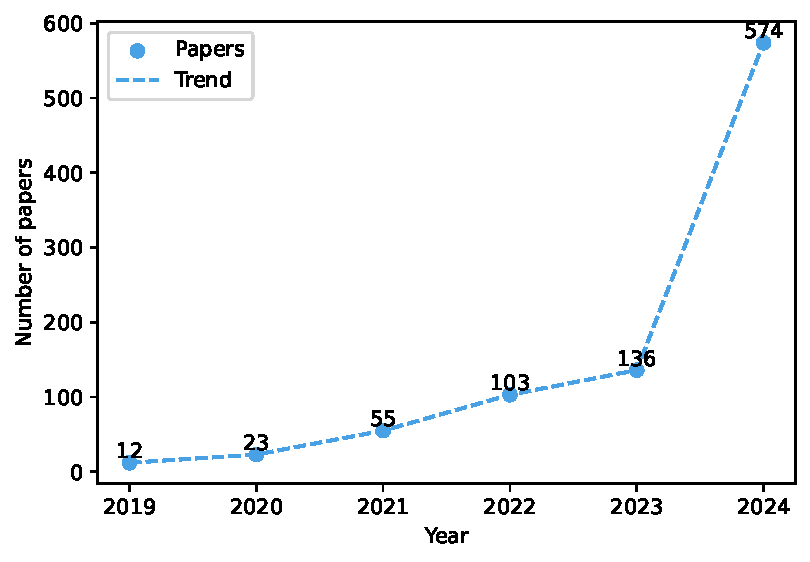
\includegraphics[width=.85\linewidth]{figures/4_related_works/taxonomy/papers_per_year.pdf}
	\label{fig:tax_papersperyear}
\end{figure}


\begin{figure}[htbp]
	\centering
	\caption{\fromsurvey{Cumulative approach of used approaches over the years.}}
	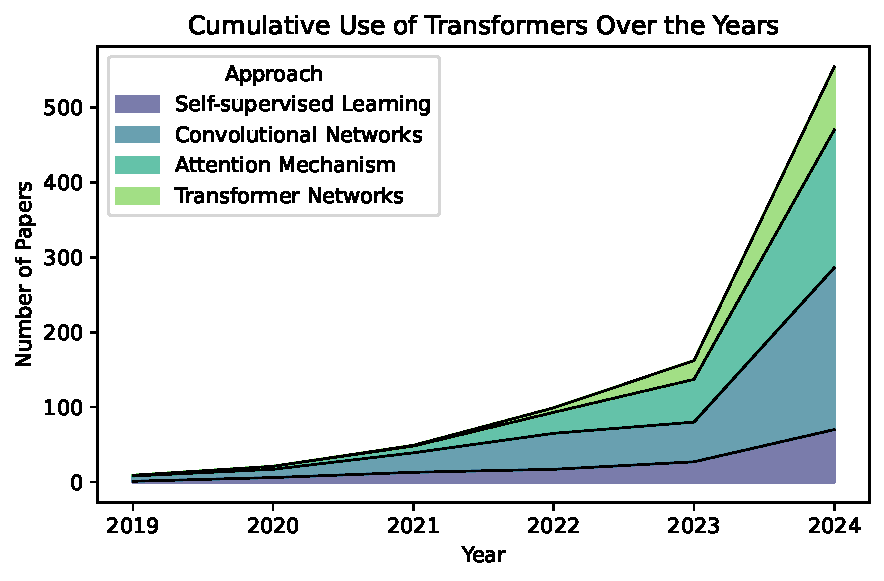
\includegraphics[width=.85\linewidth]{figures/4_related_works/taxonomy/cumulative_approaches.pdf}
	\label{fig:tax_approaches_years}
\end{figure}


\fromsurvey{As far as applications in agriculture are concerned, 503 of the 903 works referred to agriculture, i.e. $\approx. 56\%$ of all works found. To analyze their application, we created the Venn diagram in Figure \ref{fig:tax_vennapp}, which shows how frequently they are used in these 503 articles. The diagram shows that the documents related to crop mapping clearly outnumber the documents for the second most common application, change detection. The other applications appear to have been used relatively evenly for \ac{DL} research over the last five years.}

\begin{figure}[htbp]
	\centering
	\caption{\fromsurvey{Venn diagram for applications for selected papers.}}
	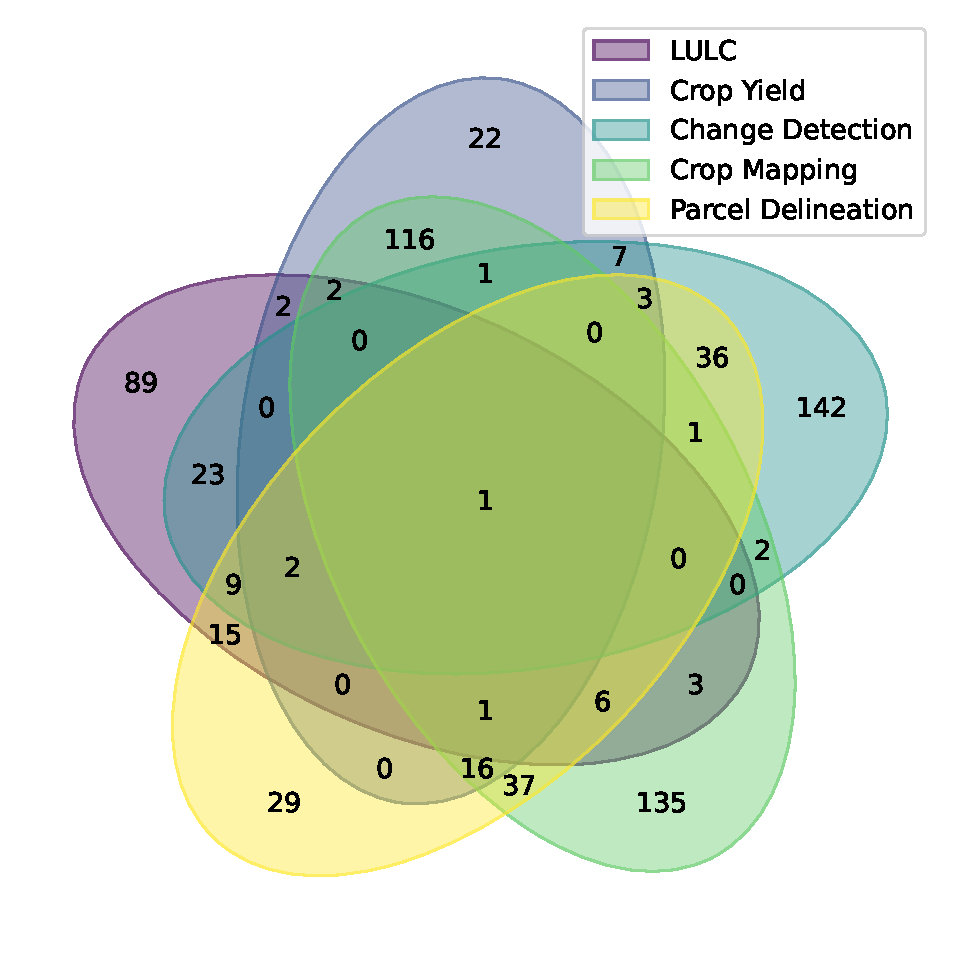
\includegraphics[width=.7\linewidth]{figures/4_related_works/taxonomy/venn_diagram_application.pdf}
	\label{fig:tax_vennapp}
\end{figure}

\fromsurvey{According to the results in Figure \ref{fig:tax_vennapp}, there are only a few overlaps between the selected topics: \ac{LULC}, Crop Yield, Change Detection, Crop Mapping, and Parcel Delineation. Although all these segments of agricultural \ac{RS} are studied separately, for some reason, they are not studied together. \ac{LULC} studies usually show agricultural classes and these studies also show forests, which together with Change Detection, can help in monitoring deforestation, such as PRODES in Brazil \citep{Almeida2022PRODES}. As for the other segments, Crop Yield, Crop Mapping, and Parcel Delineation, complement each other to form a complete and comprehensive study of \ac{RS} for agriculture \citep{sishodia2020applications}.}

\setcitestyle{super}
\begin{figure*}[!ht]
    \centering
    \caption{Proposed taxonomy for Deep Learning Remote Sensing related works.}
    \begin{tikzpicture}[
        tax_node/.style={rectangle, draw=gray!60, fill=gray!15, very thick, minimum size=5mm},align=center]
        
        \node (pic) at (0, 0) {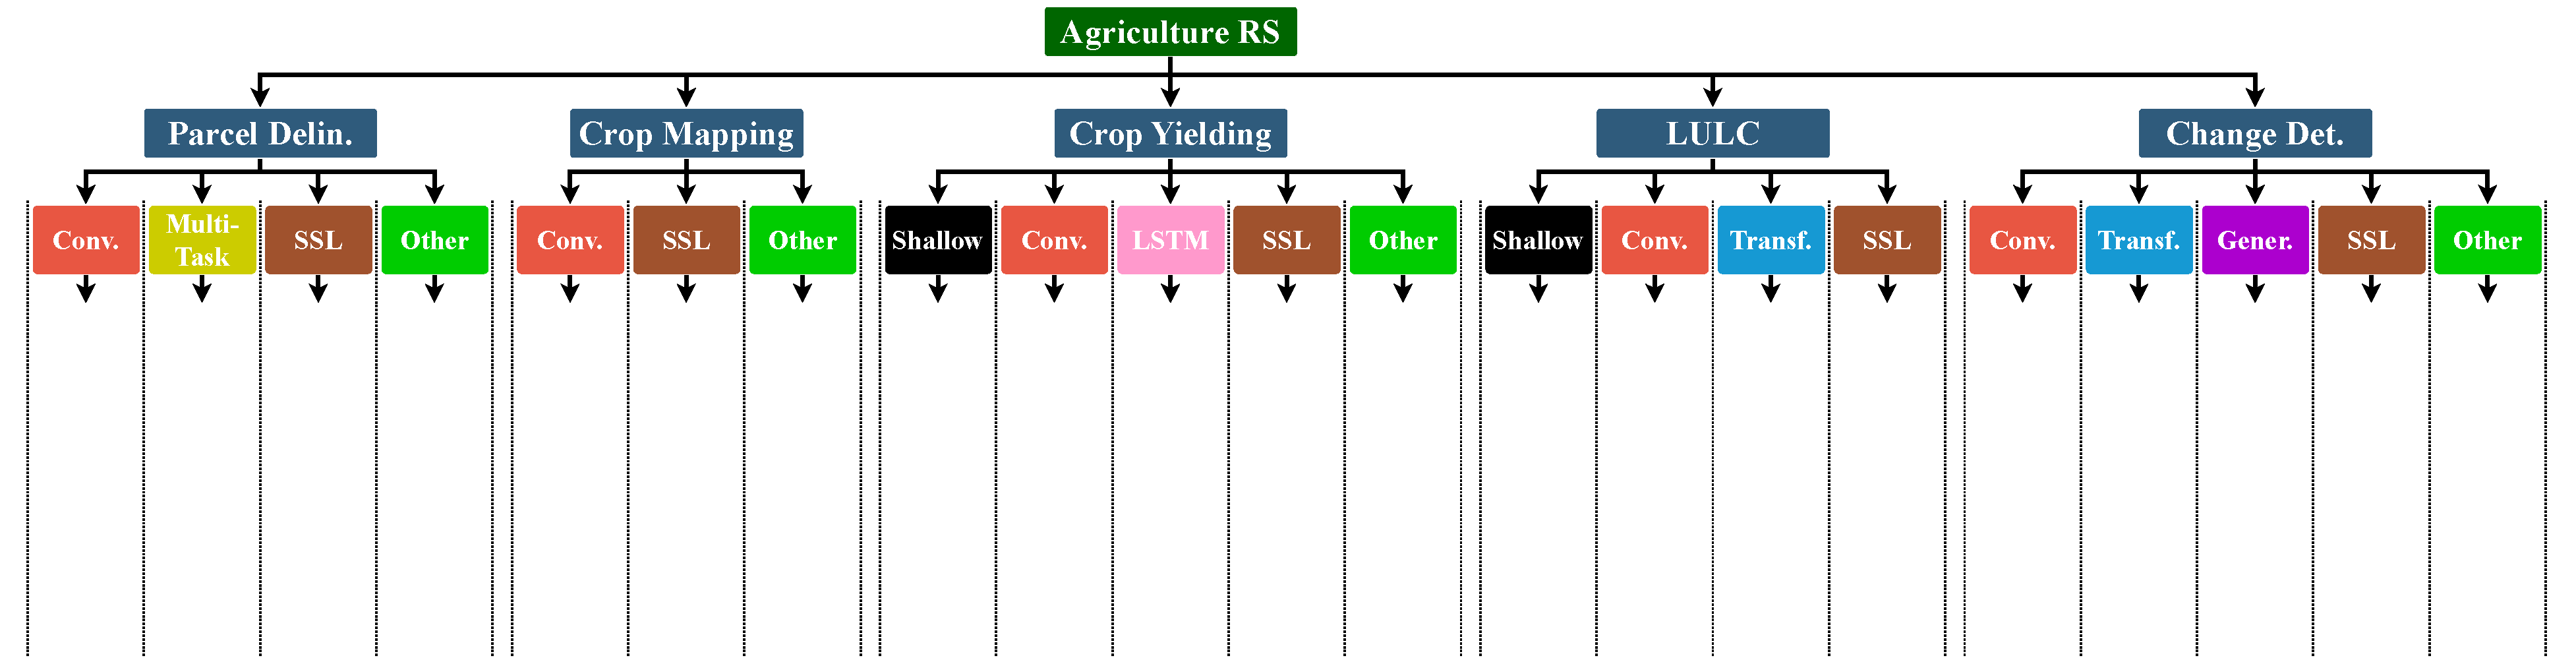
\includegraphics[clip,trim=0in -1in 0in 0in,width=\currprop]{figures/4_related_works/taxonomy/taxonomy.pdf}};
        
        %%%%%%%%%%%%%%%%%%%%%%%%%%%%%%%%%%%%%%%%%%%%%%%%%
        %%%%%%%%%%%%%%%%%%%%%%%%%%%%%%%%%%%%%%%%%%%%%%%%%
        % Parcel Segmentation.
        
        \node (parcel_conv1) at (\wparcelconv, \hfir) 
        {\refsize \cite{xu2022delineation}};
        \node (parcel_conv2) at (\wparcelconv, \hsec) 
        {\refsize \cite{xie2023edge}};
        \node (parcel_conv3) at (\wparcelconv, \hthi) 
        {\refsize \cite{zhang2023novel}};
        \node (parcel_conv4) at (\wparcelconv, \hfou) 
        {\refsize \cite{waldner2020deep}};
        
        \node (parcel_mt1) at (\wparcelmt, \hfir) 
        {\refsize \cite{li2023using}};
        \node (parcel_mt2) at (\wparcelmt, \hsec) 
        {\refsize \cite{yan2024tsanet}};
        \node (parcel_mt3) at (\wparcelmt, \hthi) 
        {\refsize \cite{10664585}};
        \node (parcel_mt4) at (\wparcelmt, \hfou) 
        {\refsize \cite{zhao2023fastsegment}};
        \node (parcel_mt5) at (\wparcelmt, \hfif) 
        {\refsize \cite{10644049}};
        
        \node (parcel_ssl1) at (\wparcelssl, \hfir) 
        {\refsize \cite{calhoun2022self}};
        
        \node (parcel_other1) at (\wparcelother, \hfir) 
        {\refsize \cite{huang2022unsupervised}};
        \node (parcel_other2) at (\wparcelother, \hsec) 
        {\refsize \cite{osco2023segment}};
        \node (parcel_other3) at (\wparcelother, \hthi) 
        {\refsize \cite{kerner2024multi}};

        %%%%%%%%%%%%%%%%%%%%%%%%%%%%%%%%%%%%%%%%%%%%%%%%%
        %%%%%%%%%%%%%%%%%%%%%%%%%%%%%%%%%%%%%%%%%%%%%%%%%
        % Crop Mapping.
        
        \node (mapping_conv1) at (\wmappingconv, \hfir) 
        {\refsize \cite{yaramasu2020pre}};
        \node (mapping_conv2) at (\wmappingconv, \hsec) 
        {\refsize \cite{xu2020deepcropmapping}};
        \node (mapping_conv3) at (\wmappingconv, \hthi) 
        {\refsize \cite{gallo2021sentinel}};
        \node (mapping_conv4) at (\wmappingconv, \hfou) 
        {\refsize \cite{farmonov2023crop}};
        \node (mapping_conv5) at (\wmappingconv, \hfif) 
        {\refsize \cite{gallo2022in_season}};
        
        \node (mapping_ssl1) at (\wmappingssl, \hfir) 
        {\refsize \cite{yuan2020self}};
        \node (mapping_ssl2) at (\wmappingssl, \hsec) 
        {\refsize \cite{yuan2022sits}};
        \node (mapping_ssl3) at (\wmappingssl, \hthi)
        {\refsize \cite{xu2024self}};

        \node (mapping_other1) at (\wmappingother, \hfir)
        {\refsize \cite{XU2021112599}};
        \node (mapping_other2) at (\wmappingother, \hsec) 
        {\refsize \cite{mena2023comparative}};
        \node (mapping_other3) at (\wmappingother, \hthi) 
        {\refsize \cite{abbas2023towards}};
        \node (mapping_other4) at (\wmappingother, \hfou) 
        {\refsize \cite{russwurm2023end}};
        \node (mapping_other5) at (\wmappingother, \hfif) 
        {\refsize \cite{mirzaei2023enhancing}};
        
        %%%%%%%%%%%%%%%%%%%%%%%%%%%%%%%%%%%%%%%%%%%%%%%%%
        %%%%%%%%%%%%%%%%%%%%%%%%%%%%%%%%%%%%%%%%%%%%%%%%%
        % Crop Yielding.
        
        \node (yielding_shallow1) at (\wyieldshallow, \hfir) 
        {\refsize \cite{huber2022extreme}};
        \node (yielding_shallow2) at (\wyieldshallow, \hsec) 
        {\refsize \cite{cheng2022wheat}};
        \node (yielding_shallow3) at (\wyieldshallow, \hthi) 
        {\refsize \cite{sabo2023deeper}};
        \node (yielding_shallow4) at (\wyieldshallow, \hfou) 
        {\refsize \cite{goel2024crop}};
        
        \node (yielding_conv1) at (\wyieldconv, \hfir) 
        {\refsize \cite{lu2024goa}};
        \node (yielding_conv2) at (\wyieldconv, \hsec) 
        {\refsize \cite{huber2024leveraging}};
        
        \node (yielding_lstm1) at (\wyieldlstm, \hfir) 
        {\refsize \cite{gavahi2021deepyield}};
        \node (yielding_lstm2) at (\wyieldlstm, \hsec) 
        {\refsize \cite{jeong2022predicting}};
        \node (yielding_lstm3) at (\wyieldlstm, \hthi) 
        {\refsize \cite{lang2023integrating}};
        
        \node (yielding_ssl1) at (\wyieldssl, \hfir) 
        {\refsize \cite{lin2023mmst}};
        
        \node (yielding_other1) at (\wyieldother, \hfir) 
        {\refsize \cite{ma2021multi}};
        \node (yielding_other2) at (\wyieldother, \hsec) 
        {\refsize \cite{liu2022rice}};
        \node (yielding_other3) at (\wyieldother, \hthi) 
        {\refsize \cite{ilyas2023automated}};
        
        %%%%%%%%%%%%%%%%%%%%%%%%%%%%%%%%%%%%%%%%%%%%%%%%%
        %%%%%%%%%%%%%%%%%%%%%%%%%%%%%%%%%%%%%%%%%%%%%%%%%
        % LULC.
        
        \node (lulc_shallow1) at (\wlulcshallow, \hfir) 
        {\refsize \cite{abdi2020land}};
        \node (lulc_shallow2) at (\wlulcshallow, \hsec) 
        {\refsize \cite{dou2024large}};
        
        \node (lulc_conv1) at (\wlulcconv, \hfir) 
        {\refsize \cite{CNN_sun2021supervised}};
        \node (lulc_conv2) at (\wlulcconv, \hsec) 
        {\refsize \cite{CNN_xu2022land}};
        \node (lulc_conv3) at (\wlulcconv, \hthi) 
        {\refsize \cite{CNN_zhan2023multi}};
        \node (lulc_conv4) at (\wlulcconv, \hfou) 
        {\refsize \cite{CNN_zhao2022cnn}};
        \node (lulc_conv5) at (\wlulcconv, \hfif) 
        {\refsize \cite{AT_zhu2021spectral}};
        \node (lulc_conv6) at (\wlulcconv, \hsix) 
        {\refsize \cite{farmonov2023crop}};
        \node (lulc_conv7) at (\wlulcconv, \hsev) 
        {\refsize \cite{AT_zheng2022rotation}};
        
        \node (lulc_transf1) at (\wlulctransf, \hfir) 
        {\refsize \cite{TRAN_sun2022spectral}};
        \node (lulc_transf2) at (\wlulctransf, \hsec) 
        {\refsize \cite{yao2023extended}};
        
        \node (lulc_ssl1) at (\wlulcssl, \hfir) 
        {\refsize \cite{tarasiou2022embeddingearthselfsupervisedcontrastive}};
        \node (lulc_ssl2) at (\wlulcssl, \hsec) 
        {\refsize \cite{moore2023selfsupervisedapproachlandcover}};
        \node (lulc_ssl3) at (\wlulcssl, \hthi) 
        {\refsize \cite{calhoun2022self}};
        \node (lulc_ssl4) at (\wlulcssl, \hfou) 
        {\refsize \cite{moore2023selfsupervisedapproachlandcover}};
        \node (lulc_ssl5) at (\wlulcssl, \hfif) 
        {\refsize \cite{XUE2025110959}};

        %%%%%%%%%%%%%%%%%%%%%%%%%%%%%%%%%%%%%%%%%%%%%%%%%
        %%%%%%%%%%%%%%%%%%%%%%%%%%%%%%%%%%%%%%%%%%%%%%%%%
        % Change Detection.
        
        \node (change_conv1) at (\wchangeconv, \hfir) 
        {\refsize \cite{gao2019change}};
        \node (change_conv2) at (\wchangeconv, \hsec) 
        {\refsize \cite{li2021combined}};
        \node (change_conv3) at (\wchangeconv, \hthi) 
        {\refsize \cite{song2022csanet}};
        \node (change_conv4) at (\wchangeconv, \hfou) 
        {\refsize \cite{ye2023adjacent}};
        \node (change_conv5) at (\wchangeconv, \hfif) 
        {\refsize \cite{miao2023snunet3+}};
        \node (change_conv6) at (\wchangeconv, \hsix) 
        {\refsize \cite{huang2023smads}};
        
        \node (change_transf1) at (\wchangetransf, \hfir) 
        {\refsize \cite{chen2021remote}};
        \node (change_transf2) at (\wchangetransf, \hsec) 
        {\refsize \cite{yan2023transy}};
        \node (change_transf3) at (\wchangetransf, \hthi) 
        {\refsize \cite{shafique2023ssvit}};
        \node (change_transf4) at (\wchangetransf, \hfou) 
        {\refsize \cite{zhang2023multi}};
        \node (change_transf5) at (\wchangetransf, \hfif) 
        {\refsize \cite{tang2024siamese}};
        \node (change_transf6) at (\wchangetransf, \hsix) 
        {\refsize \cite{chen2024visiontwinnet}};
        
        \node (change_gen1) at (\wchangegen, \hfir) 
        {\refsize \cite{du2019unsupervised}};
        \node (change_gen2) at (\wchangegen, \hsec) 
        {\refsize \cite{tang2021unsupervised}};
        
        \node (change_ssl1) at (\wchangessl, \hfir) 
        {\refsize \cite{tao2023tov}};
        \node (change_ssl2) at (\wchangessl, \hsec) 
        {\refsize \cite{feng2024feature}};
        
        \node (change_other1) at (\wchangeother, \hfir) 
        {\refsize \cite{10460113}};
        \node (change_other2) at (\wchangeother, \hsec) 
        {\refsize \cite{hou2019w}};
        \node (change_other3) at (\wchangeother, \hthi) 
        {\refsize \cite{du2023concatenated}};
        \node (change_other4) at (\wchangeother, \hfou) 
        {\refsize \cite{zhao2023triple}};
        \node (change_other5) at (\wchangeother, \hfif) 
        {\refsize \cite{bandara2024ddpmcddenoisingdiffusionprobabilistic}};
        \node (change_other6) at (\wchangeother, \hsix) 
        {\refsize \cite{wen2024gcdddpmgenerativechangedetection}};
        \node (change_other7) at (\wchangeother, \hsev) 
        {\refsize \cite{jia2024siamesemeetsdiffusionnetwork}};
        
    \end{tikzpicture}
    \fromsurvey{Classification of the selected articles under the proposed categories of the taxonomy presented in this work. Each category can be further divided into more refined groups according to the methods' characteristics. Each method may fall under more than one group, as they are not mutually exclusive.}
    \label{fig:taxonomy_paper_alocation}
\end{figure*}

\setcitestyle{authoryear, round}


\section{Parcel Delineation}
\label{sec:parcel_segmentation}

\fromsurvey{Parcel delineation, also known as cropland delineation, is the application that separates a given region into agricultural plots. This application operates on an image or time series of images (i.e. sequence of images), aiming to output a list of polygons that circumvent agricultural tiles. In addition, the application can be seen as semantic segmentation \citep{xu2022delineation}, instance segmentation, or object detection \citep{osco2023segment}. In this sense, several traditional metrics can be used to determine the output quality, such as \ac{OA}, \ac{IoU}, \ac{mAP} and \ac{mAR}. However, agricultural plots can be quite irregular, which means that such metrics do not represent the quality of model predictions very well, since they were designed for Bounding Boxes. For this purpose, the GTC error metric \citep{LONG2022102871} based on object detection was developed, which considers the over- and underclassified areas, weighing them according to the areas of each plot.}

\fromsurvey{Recently, the \Acf{SAM} was introduced and adapted to the \ac{RS} context \citep{osco2023segment}. Preliminary tests using \ac{VHR} and \ac{UAV} imagery demonstrated its potential. However, it has not been tested on \ac{LR}, \ac{MR}, or \ac{HR} images, and all the datasets evaluated by the authors were derived from \ac{UAV} sensors. The authors also highlighted the need for auxiliary inputs, such as text or bounding boxes, refining the predictions, and recommending further investigation of the model's applicability to \ac{RS}. It is important to note that, using \ac{SAM}, the \ac{SAM} UKFields project generated a dataset of agricultural plots (see Table \ref{tab:context_labeled_datasets}) for the regions of England, Wales, Scotland, and Northern Ireland using harmonic terms from MSI/Sentinel-2 \ac{NDVI} time series, regardless of the quality of this parcel delimitation has not been qualified.}

\fromsurvey{Authors generally used \acs{CNN}s or variations to delineate agricultural parcels. \cite{xu2022delineation} used a U-Net with separable depth-wise convolution layers called DSCUnet to raw segment and classify agricultural areas, then, a Richer Convolutional Features Network was employed to refine the boundary delineation of the parcels from agricultural classified regions obtained by the former step, using single \ac{VHR} images from the Gaofen-2 satellite. The authors pointed to misclassification issues when the study area contains small buildings close to agricultural parcels. \cite{xie2023edge} propose the High-Resolution Network (HRNet), a \ac{CNN} integrated with an attention module that retains feature information at different scales via parallel multiresolution branches. These branches are merged and fed into two modules: (i) an object-contextual module, which enhances the representation of contextual information and outputs parcel edge results, and (ii) a connectivity attention module, designed to extract connection and directional information. The outputted parcels are post-processed to merge erroneously oversegmented plots. Similarly, \cite{zhang2023novel} utilized DeepLabV3 on \ac{VHR} imagery, integrating public maps with \ac{MR} MSI/Sentinel-2 time series, to detect agricultural geometries using sequences of \ac{NDVI} values. Another notable contribution in this context is the work of Waldner and Diakogiannis \citep{waldner2020deep}, who proposed a \ac{DL} approach to extract field boundaries using a modified U-Net architecture known as Fractal ResUNet. The method was designed to operate efficiently on medium-resolution satellite data such as Sentinel-2, combining convolutional layers with residual and fractal blocks to improve boundary detection in large-scale agricultural landscapes.}

\fromsurvey{However, there is a tradeoff in these methods: the better the classification of the boundaries between the plots, the smaller the plots become when compared to the labels. The closer the plots are to the original areas, the thinner their boundaries with their neighbors, and the greater the chances of merging plots incorrectly. Siamese/multi-stream architectures are a growing trend in parcel delineation to balance this tradeoff. \cite{li2023using} used a two-branched convolutional Semantic Edge-Aware multi-task Neural network (SEANet) architecture: the first branch was responsible for drawing parcels, and the second one was to fine-delimit their boundaries. The two pieces of information were combined using a multitask loss formed by a Binary Cross-Entropy and a Dice Loss to deal with class imbalance and training instability. The method was tested for single-image segmentation using Gaofen-2 and Sentinel-2 satellite imageries. \cite{yan2024tsanet} also used a dual-stream architecture with each branch using the same idea as the former paper but with \ac{SITS} as input and weighting joining the same losses instead of a simple sum, which allows choosing between better pixel-level metrics or more consistent parcels. This approach is very similar to Two-Stream Attention Network (TSANet), and both were tested in the same study region (close to the entire area of the Netherlands) with MSI/Sentinel-2, although on different datasets, achieving similar results. \cite{10664585} advanced the technique and used the frozen decoder of a simplified version of the Foundation Model called Fast\acs{SAM} \citep{zhao2023fastsegment} as the decoder of a multi-branch architecture named Two-Flow Network (TFNet), achieving a 0.6\% \ac{OA} improvement and 0.025\% GTC error reduction on the same SEANet dataset, showing that a hybrid model can work. Finally, \cite{10644049} did similar research, developing the Boundary-Field Interaction Network (BFINet) strategy but using a Pyramid Vision Transformer as a pretrained decoder in ImageNet, as well as adding modules to refine spatial details in high-level features and merge multiscale semantic information, specially designed to deal with small and irregular plots, achieving a 0.11\% improvement in \ac{OA} and 0.95\% GTC error reduction compared to SEANet, but on another dataset than the one originally used, which prevents direct comparison with TFNet.}

\fromsurvey{At last, \cite{kerner2024multi} showed that datasets do not generalize well to different regions and present that the possibility of simple Transfer Learning of a dataset from one geographic area or satellite sensor to a different target dataset may improve the metrics in the target dataset. The authors showed that this approach works best for datasets with little labeled data by improving up to 6\% the achieved F1-Score. There are also some different strategies,  \cite{huang2022unsupervised} employed an unsupervised parcel delineation using a Convolutional Graph Neural Network adapting the traditional Graph-based Unsupervised Superpixel-Aggregation method, balancing a loss function that considers both spatial and spectral affinities, generating better results than other unsupervised techniques generating results with MSI/Sentinel-2 for regions of China.}

Some self-supervised learning contrastive (see Section \ref{sec:ssl_contrastive}) methods were used as pretraining for Parcel Delineation models. Calhoun et al. \citep{calhoun2022self} showed that SwAV pretraining, first conducted on ImageNet and then with continued pretraining on \ac{RS} data, demonstrated that Transfer Learning performed in this way yields better results than the traditional approach. However, several tasks were analyzed by the authors, and the task that showed the least improvement was precisely Parcel Delineation, with only a 0.07 increase in \ac{IoU}. Furthermore, it was observed that the larger the labeled dataset, the smaller the impact of \ac{SSL} pretraining.

\fromsurvey{Finally, according to \cite{xie2023edge}, \acs{CNN}s seem to have reached their limit in this task, and researchers have begun testing new architectures. Both \cite{li2023using} and \cite{yan2024tsanet} proposed examples of the most prominent architecture focusing on dual stream and/or multitasking and removing noise from non-existent plots. The literature reports several available datasets for parcel delineation, although \cite{kerner2024multi} claims there is little geographical variety to these areas. Further, foundational models like \ac{SAM} show innovation potential but require additional research to adapt them for broader \ac{RS} applications beyond \ac{VHR} imagery.} Regarding the use of \ac{SSL} pre-training, there is very little work in this area, and only minimal improvements have been reported.

\ac{SAM}-based approaches continue to evolve, addressing limitations in zero-shot generalization for agricultural applications. \cite{xie2025fabsamfarmlandboundarydelineation} proposed fabSAM, a hybrid framework combining a Deeplabv3+-based prompter with a fine-tuned \ac{SAM} decoder. This method achieved significant improvements over zero-shot \ac{SAM}, surpassing it by 23.47\% in \ac{mIoU} on the AI4Boundaries dataset by effectively generating mask and point prompts from intermediate segmentation outputs. Concurrently, \cite{lavreniuk2025delineateflowfastcountrylevel} introduced Delineate Anything (DelAny), an instance segmentation model based on YOLOv11 and trained on the massive FBIS-22M dataset (22.9 million field instances). DelAny demonstrated superior zero-shot performance across diverse agro-ecological zones, achieving over 100\% higher \ac{mAP} and 400$\times$ faster inference compared to SAM2. This resolution-agnostic approach reformulates delineation as instance segmentation to prevent field merging, enabling the generation of topologically consistent national-scale maps.

\section{Crop Mapping}
\label{sec:crop_mapping}

\fromsurvey{Crop mapping is the application in which, given a parcel or a map, a classification per parcel or pixel is generated for certain crops, usually using a time series of \ac{RS} images. Datasets from a given region may not generalize well to other areas due to climatic or agricultural calendar differences \citep{gadiraju2023remote}. Crop mapping is usually divided between (i) post-harvest, with the season already complete, and (ii) in-season classification, also called early prediction.}

\subsection{Post-harvest classification}

\fromsurvey{Post-harvest classification is the sub-application of Crop Mapping in which the result is obtained after the harvest, i.e. with all available agricultural time series data. This sub-application is more common in the literature, as it is simpler due to the greater amount of data available.}

\fromsurvey{CNNs are one of the most used strategies for Crop Mapping, as in \cite{gallo2021sentinel} that used a 3D \ac{CNN} Features Pyramid Network to classify \ac{SITS} crops pixel-wise using multispectral images from MSI/Sentinel-2, using a CELoss to construct the Crop Parcels and an MSELoss to determine in which time interval it is more probable to be Crop Season. Integrating attention mechanisms in a \ac{CNN} is the strategy adopted by \cite{farmonov2023crop} to extract long-term features and classify crops at the pixel level, achieving 97.89\% of \ac{OA} with hyperspectral images. The method proposed by \cite{yaramasu2020pre} used a bidirectional Long Short-Term Memory (LSTM) with a convolutional structure for generating embeddings as a temporal encoder with a pretrained ImageNet Very Deep Convolutional Networks (VGG), specifically in its VGG11  version\footnote{In VGG11, 11 stands for the total number of weight layers: 8 convolutional and 3 fully connected- used.} as a spatial encoder to predict crop mapping using crop rotation from previous years with Landsat \ac{SITS} as training.}

SSL pre-training was also employed in the application of Crop Mapping, especially in Transformer and post-Transformer models. \fromsurvey{MIM strategies were used. \ac{SITS}-\ac{BERT} \citep{yuan2020self} leverage generative pretraining for \ac{BERT} models via masking a pixel \ac{SITS} with high-value pixels to simulate clouds and training the network for reconstructing it. \ac{SITS}-\ac{BERT} proposes a modification of the transformer's positional encoder to incorporate the \ac{DoY} in order to integrate information from the agricultural calendar. Like all other \ac{SSL} methods, the pretraining is followed by fine-tuning to incorporate semantic information about crop types. \cite{yuan2022sits} further refined their strategy by using a convolutional transformer architecture to handle time series of 5x5 patches. The pretraining followed the same methodology, seeking to reconstruct the central pixel of each patch. The results were slightly better than the predecessor model, achieving an improvement of approximately 1.7\% in \ac{OA}.}

\fromsurvey{There are also contrastive \ac{SSL} models in Crop Mapping that pretrain transformer backbones. Xu et al. \citep{xu2024self} used them for Post-harvest Crop Classification, creating the model \ac{SITS}-MoCo, in which the band values are used as input series in the transformer, while the \ac{DoY} is used as input order for Positional Encoding, in addition to \ac{NDVI} Seq2Vec as pooling to reduce dimensionality in the time series to use the information in the classification head. As pretraining, MoCo was used, wherein multiple domain-specific augmentations were employed, including removal of random bands, random band switches, displacement of the time series, and changes in timestamp values, among others. The authors states that the model achieves state-of-the-art performance, even when compared to modern Masked Image Modeling methods \citep{yuan2020self,yuan2022sits}.} More recently, building upon the of \ac{SITS}-\ac{BERT}, \cite{shravan2024sits} introduced \ac{SITS}-BERT++, incorporating a dual activation function strategy, utilizing Swish for the overall model architecture to improve gradient flow, while retaining GeLU for the classification \ac{MLP}. Additionally, temporal data augmentations were also used. Also, a multihead attention mechanism was used in the top of the model in the pre-training reconstruction stage. These enhancements resulted in an improvement of nearly 3\% \ac{OA}    on the California dataset compaired to the original \ac{SITS}-\ac{BERT} \citep{yuan2020self}.

\subsection{In-season classification}

\fromsurvey{In-season classification is the sub-application of crop mapping that produces the result before the harvest. It is usually desirable to correctly classify crops as early as possible, given the economic advantages, especially with the reduced use of satellite images, which provides a cost reduction. It is a more complex application than post-harvest classification, as there is less data available.}

\fromsurvey{Several approaches focus on early recognition using \acs{CNN}s and recurrent models, as \cite{gallo2022in_season} that utilized a 3D \ac{CNN} to classify parcels over time, enabling early-season predictions. \cite{yaramasu2020pre} employed a bidirectional ConvLSTM for in-season crop mapping. \cite{xu2020deepcropmapping} developed an \ac{LSTM} capable of making predictions both during and after the season, with minimal performance differences between early and late predictions.}

\fromsurvey{\cite{russwurm2023end} presented a classification head that can be attached to any \ac{SITS} crop mapping model, allowing for in-season crop mapping. This classification head outputs the probability of the classification being correct given the number of timestamps compared to the full season, trained with an Earliness-Rewarded Loss, turning the model into a multimodal approach. The methodology was tested with an \ac{LSTM} model, being able to predict the Crops using from 16\% to 40\% of the \ac{SITS}.}

\subsection{Mixed strategies}

\fromsurvey{It is worth mentioning some other mixed strategies also researched. For example, \cite{abbas2023towards} proposed a temporal encoder capable of learning a crop mapping representation from a given region, then retrained in another area with a different agricultural calendar, done by transformers PE output computed on the source region is used as a proxy to quantify the temporal shift concerning the PE output obtained on the target region.}

\fromsurvey{An extensive analysis of the interpretability of Crop Mapping models presented by \cite{xu2024new} showed that the most significant band for crop differentiation is usually \acs{SWIR}1 ($\approx$ 1600nm). Additionally, the authors claim that, when trained with the entire season, the last timestamps are mostly widely used for prediction rather than early parts of the season. \cite{XU2021112599} proposed a Bayesian Active Learning Network capable of identifying which samples have to be labeled to represent a greater increase in information from the dataset, which can help reduce high labeling costs.}

\fromsurvey{\cite{yang2022ppce} designed a new loss function called Phenological Prior Cross Entropy (PPCE) based on traditional \ac{CELoss}, which weights probabilities based on \ac{NDYI} to capture the common yellowness of the flowering period of crops and on \ac{NDVI} for the senescence period. It prioritizes the correction of misclassified pixels based on phenological likelihood. }

\fromsurvey{\cite{mena2023comparative} tested the fusion of optical and \ac{SAR} data, as well as climatological data for Crop Mapping. It was reported that the fusion of these data types improves classification, especially with feature-level fusion using gates, resulting in a 0.34\% improvement in accuracy on the tested datasets. \cite{mirzaei2023enhancing} also employed Data Fusion, but only between \ac{SAR} and optical data; they created tabular features and used a Conditional Adversarial Generative Network (CTGAN) to generate synthetic data of the most underrepresented classes.}

\section{Crop Yielding}
\label{sec:crop_yielding}

\fromsurvey{Crop yield prediction is a regression application that typically uses the geometry of a crop region and the growth cycle dates to forecast production. Several methods combine satellite images with other sources of information, such as weather data and soil information. It is a difficult application to generalize, and there is little amount of datasets for it, which means that Shallow Learning is still used in addition to \ac{DL} techniques, as stated by \cite{goel2024crop}. Moreover, methodologies are rarely directly compared, as many datasets are private. Therefore, various techniques are used to address the issue of limited data volume.}

\fromsurvey{Shallow learning methods are still widely used. \cite{huber2022extreme} compared two \ac{DL} methodologies, \ac{CNN} and \ac{CNN} \ac{LSTM}, with the Shallow Learning XGBoost methodology for soybean crop yield, concluding that the traditional method performed better. However, the authors also claimed that larger datasets can improve the metrics of \ac{DL} techniques. \cite{sabo2023deeper} compared shallow and \ac{DL} methods, concluding that traditional ones performed better in their experiments due to the small size of the available dataset for barley, durum, and soft wheat crop yielding. \cite{cheng2022wheat} also compared the traditional techniques, Random Forest, Gradient Boosting Decision Tree, used in the XGBoost framework, and \ac{SVM} with \ac{LSTM} concluding that the \ac{LSTM} model performs better in the winter wheat forecast using data from MSI/Sentinel-2.}

\fromsurvey{\cite{ilyas2023automated} used a hybrid set of \ac{DL} feature extractors with a fuzzy bagging classifier composed of shallow learning methods for crop yield. The authors aimed to forecast several types of crops (flaxseed, lentils, rice, sugarcane, and wheat) using satellite imagery and climate data. As there was little data available, they used a set of techniques to increase the generalization of the learned representation. In the same direction, \cite{ma2021multi} used a Bayesian Neural Network, which is known to increase the model's generalization, allowing a more successful Transfer Learning. The authors tested the methodology in the USA Corn Belt forecasting.}

\fromsurvey{\cite{lu2024goa} used a \ac{CNN} BiGRU network with attention layers to predict soybeans for a county-level in USA based on SR data, climate data, and photosynthetic-related parameters. \cite {khaki2021simultaneous} also used an end-to-end \ac{CNN} that forecasts, at the same time, Soy and Corn crops. The architecture has two regressors using the same shared backbone, predicting when the crops are ready for harvest. \cite{huber2024leveraging} presented some Deep Transfer Learning techniques in \acs{CNN}s to overcome catastrophic forgetting and negative transfer problems. The Transfer Learning example is the adaptation of the US soybean yield prediction to the Argentina soybean yield prediction with MSI/Sentinel-2 data.}

\fromsurvey{Some architectures used \ac{LSTM} to handle temporal dependencies of Crop Yielding. In that direction, \cite{jeong2022predicting} used a mixed \ac{LSTM} architecture with \ac{CNN} based on \ac{MODIS} imagery, meteorological data, and geographic data (geographic coordinates and country identifier) for early prediction (two months before the harvest). \cite{gavahi2021deepyield} used a similar architecture with 3D \acs{CNN}s and the addition of Land Cover information provided by \ac{MODIS}. \cite{lang2023integrating} compared \ac{LSTM} with Shallow Learning methods, concluding that \ac{LSTM} presents better results for county-level early prediction cotton forecasting.}

\fromsurvey{Improving temporal dependencies, \cite{liu2022rice} presented a Transformer architecture followed by a convolutional layer using satellite and environmental data, also presenting a graphical analysis of the explainability of attention mechanisms, predicting rice yield two months before harvest.} 

\acs{ViT}s were also used, but through contrastive \ac{SSL} pretraining (see Section \ref{sec:ssl_contrastive}). \cite{lin2023mmst} \fromsurvey{presented a Multi-Modal Spatial-Temporal Vision Transformer which employs a multi-modal transformer trained with Sentinel-2 and weather data, claiming that the method is climate-aware. The multimodal pretraining approach presented better results than the Convolutional \ac{LSTM} hybrid models in experiments with multiple \ac{RS} imaging modalities, with pretraining using the standard \ac{SimCLR} used as a baseline.}

\section{Land Use and Land Cover}
\label{sec:lulc}

\fromsurvey{\Acf{LULC} is a semantic segmentation application in which, given an \ac{RS} image or mosaic, it classifies the image into labels, such as water bodies, bare soil, vegetation, forest and urban areas \citep{Brandt2009}. Producing \ac{LULC} maps is one of the most common tasks using \ac{RS} data. It is useful for generating classification maps \citep{8518619}, and it is possible to notice geographic changes by comparing them over time. \ac{LULC} studies are useful for agricultural purposes as they enable, for example, monitoring changes in water bodies, soil deterioration, deforestation, or even road construction.}

\fromsurvey{Shallow Learning continued to be used in some situations for \ac{LULC}, especially \ac{LR}/MR satellites. Abdi \citep{abdi2020land} compared traditional methods (Support Vector Machine, XGBoost, and RF) with an FFN with Tanh activation, and concluded that SVM performs better (OA 75.8\% ± 1.7\%) and that the worst model in the experiment is \ac{DL} (OA 73.3\% ± 0.23\%) using MSI/Sentinel-2 time series. \cite{dou2024large} argued that the limited amount of multispectral bands in Landsat missions leads \acs{CNN}s to problems in stable features from the spectral domain; hence, they presented a hybrid methodology called deep-shallow learning that uses \acs{CNN}s to receive raw Landsat images and generate Deep Features for several Shallow Learning Classifiers, whose output probabilities are inserted into another \ac{CNN} to effectively generate \ac{LULC}, generating an \ac{OA} of 88.95\% against 84.97\% for a 1D-CNN.}

\fromsurvey{For \ac{LULC} applications, \acs{CNN}s were also used. \cite{CNN_sun2021supervised} introduced an end-to-end Fully Convolutional Segmentation Network for \ac{HSI} classification. The FCSN addresses the limitations of traditional \ac{CNN}-based methods, particularly their poor generalization capabilities and coarse labeling of \ac{HSI} cubes. Unlike traditional methods that focus on the center pixel, this method classifies all pixels in an \ac{HSI} cube simultaneously. \cite{CNN_xu2022land} introduced an interactive segmentation network that leverages user input to improve land cover mapping accuracy in high-resolution images, showcasing significant advancements over purely automatic methods. \cite{CNN_zhan2023multi} improved accuracy through multiscale feature reconstruction and interclass attention weighting, addressing issues such as ambiguous boundaries and intraclass variance. Building on this foundation, Zhao \citep{CNN_zhao2022cnn} evaluates various \ac{DL} architectures, concluding that 3D \acs{CNN}s and \acs{ViT}s are most effective for spatio-temporal representation in \ac{RS} time series, highlighting the utility of both optical and \ac{SAR} images for land cover classification. Integrating attention mechanisms in \acs{CNN}s with \ac{HSI} images has significantly improved accuracy and feature extraction. \cite{AT_zhu2021spectral} incorporated a global joint attention mechanism to improve spectral and spatial feature discrimination, achieving superior classification accuracy under challenging conditions. Similarly, \cite{farmonov2023crop} applied a Wavelet-Attention on \ac{CNN} with a spectral attention mechanism to improve crop type mapping accuracy, demonstrating the effectiveness of attention modules in agricultural monitoring. Furthermore, \cite{AT_zheng2022rotation} employed a rotation-invariant attention network to address rotational variances in \ac{HSI} data, showcasing the flexibility and robustness of attention mechanisms to improve classification performance.}

\fromsurvey{Transformers started to be used for the \ac{LULC} application.  \cite{TRAN_sun2022spectral} presented a method combining the \ac{CNN} and transformer model. They used 3D and 2D convolutions for low-level feature extraction, a Gaussian-weighted tokenizer for feature transformation, and a transformer encoder for deep feature representation. Compared to traditional \ac{CNN} methods, this method improved semantic feature extraction, reduced computational costs, and showed better experimental results on standard datasets.  \cite{yao2023extended} also used Transformers but in a multimodal approach to include heterogeneous \ac{RS} data, using parallel branches of position-shared \acs{ViT}s extended with separable convolution modules, each branch made to process a type of data. Using a dataset with hyperspectral and LiDAR data and balancing the weights of each branch, the \ac{OA} was 88.95\% \textit{versus} 87.71\% only for hyperspectral data.}

\fromsurvey{Contrastive \ac{SSL} (see Section \ref{sec:ssl_contrastive}) has also been used in \ac{LULC}. Tarasiou and Zafeiriou \citep{tarasiou2022embeddingearthselfsupervisedcontrastive} adapted to MoCo, also with a queue for negative samples, generating the segmentation map using single images. As augmentations, random selections of time series images were used, in addition to horizontal and vertical flips. A single georeferenced pixel is treated as a positive pair, while all other pixels are treated as negative pairs. The method achieves an improvement of up to 25\% absolute \ac{mIoU} over the same architecture without pretraining.}

\fromsurvey{LULC has also benefitted from MIM (see Section \ref{sec:ssl_mim}) strategies.  \cite{XUE2025110959} employed a \acs{ViT} that receives hyperspectral multitemporal data, height data, and \ac{VHR} images to create land use and coverage maps. As a pretraining strategy, the authors modify MAE to receive these three inputs and apply cross-attention across their representations. The downstream classifier is trained using shallow learning on the frozen features extracted by the \acs{ViT}, thus being a hybrid method.}

\fromsurvey{LULC studies large and heterogeneous area datasets, and the target mapping labels usually include natural or anthropized classes. Even considering only farms, it is possible to identify several classes, such as water bodies, buildings, roads, farmlands, and forests. The application has been using SL for \ac{LR}/MR due to the low number of features possible to be generated \citep{dou2024large}. As for \ac{HR}/VHR or hyperspectral satellites, the research area has been following closely the area of computer vision, replacing traditional \acs{CNN}s \citep{CNN_sun2021supervised} with versions with attention modules \citep{AT_zheng2022rotation} or even using Transformers \citep{TRAN_sun2022spectral, yao2023extended}}, possibly using or not using \ac{SSL} pre-training.

\section{Change Detection}
\label{sec:change_detection}

\fromsurvey{In \ac{RS}, Change Detection is the classification of dissimilarities in the region of interest, given two, or more, timestamps as input according to  \cite{rs14040871}, producing a classification map identifying the pixels that most likely changed.  \cite{diniz2015deter} stated that, in agriculture, it is quite common for detecting deforestation and fire scars, but it can also detect crop areas or river floods. Such an application is vital for active earth observation monitoring in near real-time. Generally, the papers include tests with datasets that involve both Change Detection of buildings and useful data for agriculture.}

\fromsurvey{Many convolutional models have been used, especially in symmetric and/or siamese networks, which are useful for comparing two different instances as proposed by  \cite{li2021combined} and by  \cite{ye2023adjacent}. Some methods even use adaptations of architectures widely used in \ac{RS}, like U-Net-based methods presented by  \cite{miao2023snunet3+} and by  \cite{huang2023smads}. These architectures tend to perform well, however, they do not exhibit gradual performance improvements with large volumes of data like the transformer-based ones, and they tend to perform worse than them. Several types of \ac{RS} data are used. For example,  \cite{gao2019change} presented a Deep Cascade Network for Change Detection using \ac{SAR} images. This data is quite interesting as it penetrates clouds. Due to the speckle noise in \ac{SAR} data and increasing network depth, exploding gradients and overfitting are common. To address this, residual learning with fusion mechanisms is used in \acs{CNN}s. The methodology presents better results when compared to similar ones that also use \ac{SAR}, which were all evaluated on a farmland dataset.}

\fromsurvey{Some methodologies also use convolutional networks with attention mechanisms, such as the method proposed by  \cite{song2022csanet} that works with hyperspectral images using a symmetric network, aiming for Bi-Temporal Change Detection, using self-attention on each image, and cross-temporal attention to integrate their different features. The method outperforms state-of-the-art models in the three datasets tested: irrigated agriculture, wetland agriculture, and river movement.}

\fromsurvey{Various methodologies were used for Change Detection with transformers, although often in hybrid form with other models \citep{shafique2023ssvit, zhang2023multi, tang2024siamese, chen2024visiontwinnet}.  \cite{chen2021remote} used a symmetric architecture that mixes a ResNet without its last layer (as a backbone) and a transformer as an encoder/decoder to highlight the most relevant semantic features of each image to be compared and classified pixel-wise using an \ac{FCN}. The methodology performed satisfactory outcomes, as the semantic features highlight modified objects in each dataset, such as buildings in a city dataset or rivers in a geographic change dataset.  \cite{yan2023transy} achieved even better results using a symmetric architecture with a Swin Transformer as the backbone and a Progressive Attention Module method for pixel-wise classification of image changes.}

\fromsurvey{The unsupervised learning paradigm was used by \cite{du2019unsupervised} that proposed a symmetric network model but with an unsupervised method that selects pixels that have changed with high confidence for pseudo-label generation. In the same direction, \cite{tang2021unsupervised} also used an unsupervised methodology, though they used GNN (Graph Neural Networks) as the model and Metric Learning to produce pseudo-labels.}

\fromsurvey{Alternative architectures and other paradigms were employed as well. \cite{du2023concatenated} used generative pretraining for optical and \ac{SAR} data separately, followed by U-Net++ for Change Detection. GANs (Generative Adversarial Networks) were used by \cite{hou2019w} and by \cite{du2023concatenated} for pixel-wise classification, converting the problem from Change Detection to Image Translation. \cite{zhao2023triple} employed data fusion within the methodology for classifying change detection.}

\fromsurvey{More recently, diffusion model methodologies have also been used. \cite{bandara2024ddpmcddenoisingdiffusionprobabilistic} used a U-Net trained to remove synthetic noise added to RGB MSI/Sentinel-2 images, creating a model capable of generating \ac{RS} images. This network was duplicated with its weights frozen (similar to a Siamese Network), and a simple classifier that uses features generated for a before-and-after image was trained to predict the Change Detection map. \cite{wen2024gcdddpmgenerativechangedetection} presented a methodology that claimed itself as an evolution of the previously presented model, using a diffusion model to predict the Change Detection map with end-to-end training. \cite{10460113} presented an evolution of the second presented model, but using a hybrid Transformer-Convolutional model as a noise remover instead of a U-Net. \cite{jia2024siamesemeetsdiffusionnetwork} were also inspired by the first model, although their research moved towards a different direction: they used a feature extractor that does not use diffusion, and given its input features, trained a diffusion U-Net to generate the Change Detection map.}

\fromsurvey{At last, \ac{SSL} contrastive pretraining (see Section \ref{sec:ssl_contrastive}) has reached Change Detection. \cite{tao2023tov} used a mean teacher distillation approach, wherein the teacher has its weights updated with an exponential moving average. In addition, using domain knowledge, negative hard samples are chosen and weighted based on the similarity between the embeddings with the positive pairs, thus reducing the number of negative samples needed. \cite{feng2024feature} directly modified Barlow Twins for the context of Change Detection. Instead of creating the correlation matrix between pairs of views of the same image, it creates it from a pair of absolute differences between a timestamp before and a timestamp after some change. In this way, the model is encouraged to learn features that represent changes that may occur in pairs of images from the same region acquired at distinct times. Furthermore, authors pair the original Barlow Twins loss with loss components that ensure robustness to radiometric and lighting variations, in addition to a temporal consistency regularization.}

\section{Discussion About Literature}\label{sec:rdiscussion}

\fromsurvey{In sum, the results of this paper indicate that agricultural remote sensing has indeed undergone quite profound changes during the time covered by the papers. First, the most common methods are no longer Shallow Learning \citep{sabo2023deeper}, and the community seemed to have migrated to \ac{DL} \citep{xu2022delineation} in all applications defined in the Taxonomy (Section \ref{sec:taxonomy}). This change confirms the prediction made by \cite{kamilaris2018deep} in 2018. This is due to the reasons for this same change in traditional computer vision: 1) better training strategies for deeper networks \citep{krizhevsky2012imagenet}; 2) increased computational capacity, largely based on the adoption of the use of \acs{GPU}s instead of CPUs; and 3) the considerable increase in the amount of data \citep{deng2009imagenet}, in addition to advances in\ac{RS} technologies. Nowadays, \ac{DL} models for remotely sensed data can leverage the number of available satellites, together with the advances in their spatial, temporal and spectral resolutions (see Table \ref{tab:context-satellites}). One approach that has proven to be highly effective in leveraging these points is fusion models \citep{zhao2023triple, ye2023adjacent} because it is now possible to use a greater variety of sensors together and provide more datasets and, therefore, more analyses in remote sensing of agriculture.}

\fromsurvey{Another field that is leveraging the mentioned points above is self-supervised learning, even though the use of \ac{SSL} is still emerging in \ac{RS} in general \citep{xu2024self, wang2024decoupling, xiong2024neural}. In general, \ac{SSL} for remotely sensed data is utterly beneficial: remotely sensed data change in space and in time, so handcrafted labeling tends to become more expensive by the day. As a result, unlabeled data with high certainty of prediction seems to be a fair option. For this reason, all applications presented herein include methods that benefit from \ac{SSL} \citep{yuan2020self, tarasiou2022embeddingearthselfsupervisedcontrastive, calhoun2022self, lin2023mmst, tao2023tov}.}

\fromsurvey{However, the current research has mainly focused on contrastive and masking techniques, while non-contrastive techniques remain to be explored since some methods such as SimSiam \citep{chen2021exploring} and FastSiam \citep{pototzky2022fastsiam} require lower infrastructure. As with computer vision, the DL area in \ac{RS} follows the \ac{SSL} trends in a delayed manner while adapting them to incorporate domain-specific knowledge. As far as we researched, the first non-contrastive pre-training method for crop classification is proposed in this paper.}

\fromsurvey{In terms of models, the literature seems to be generally moving towards Transformer models \citep{aleissaee2023transformers} to deal with time series. The reason for this is that Transformers were the natural evolution of \ac{LSTM}s, models previously used for this type of task. This change was made because, although the \ac{LSTM} architecture is designed to handle distant dependencies, Transformers handle dependencies of any distance naturally due to their attention mechanism \citep{zhou2021informer}.  Furthermore, due to the sequential processing of \ac{LSTM} data and its natural training instability (often requiring operations such as Gradient Clipping) \citep{pascanu2013difficulty}, Transformers proved to be a great fit for \ac{SSL} pre-training thanks to their more stable training and parallel data processing. In spite of that, \acs{CNN}s \citep{farmonov2023crop} equipped with attention modules have been widely used due to its ability to focus on which bands are most important to highlight a given crop (Channel Attention) \citep{ecaNet, tang2021channel}, recalibrate the importance of the \acs{CNN}'s own internal channels (Squeeze-and-Excitation Blocks) \citep{senet} or even use the temporal attention mechanism in order to focus on the most important timestamps (Temporal Attention) \citep{li2019temporal}.}

\fromsurvey{An encountered drawback is that, especially for Crop Yielding, data are highly regionalized, presenting vast sparsity. As a result, there are still studies using Shallow Learning \citep{sabo2023deeper}, mainly with boosting models, such as XGBoost or Support Vector Machines \citep{huber2022extreme, cheng2022wheat}. These models tend to deal best with scarce labeled data due to their inherent characteristics.}

\fromsurvey{When it comes to EO sensors, the most widely used are those from the Landsat mission that can provide time series going back to 1985. The sensors in these satellites are equipped with SWIR and thermal bands that are highly efficient for studies of vegetation in general, mainly agriculture. The second most used sensor is MSI onboard Sentinel-2, which came with a better spatial and temporal resolution than the Landsat family. MODIS sensor onboard Terra and Aqua satellites can provide daily information: in spite of having a low spatial resolution, this sensor has bands that aid scientists to predict not only vegetation indices but also climate and meteorological information over the imaged area. Finally, the Sentinel-1 satellite with SAR C-band is also being highly used. This increase may be related to two factors: (i) more dissemination of remote sensing processing data for SAR, and (ii) the usage of Google Earth Engine (GEE), which provides processed SAR data and cloud processing \citep{mullissa2021sentinel1}. All these satellites are provided by either NASA or ESA; these agencies have open source policies for their data, which enables academia and companies to fully use them. Another agency with open source policy is INPE (Brazil) that, together with China, provide CBERS missions. Previous CBERS satellites have shown serious radiometric and geometric calibration errors and, for this reason, they are not widely use for studies in Brazil. However, new WFI and MUX sensors onboard INPE satellites are now corrected and have been used for studies in monitoring Amazon Rainforest \citep{almeida2022metodologiaprodes}. Moreover, commercial satellite data, such as Planet, Maxar and Airbus, are extremely expensive, which affects their popularity in research and datasets. Commercial satellite also usually have only RGB-NIR, which limitates their application in agriculture, even though their very high resolution are recommended for parcel delineation.}

\fromsurvey{There are few datasets for remote sensing in agriculture in the literature (see Table \ref{tab:context_labeled_datasets}), especially considering that the applications usually do not generalize well regionally. However, there are several studies that indicate that Transfer Learning - i.e. supervised pretraining - can be used and improves the quality of the models. Comparing studies in the literature can be tricky as authors rarely use the same datasets. Therefore, there is a need to create larger and global datasets for benchmarking, perhaps by pooling multiple datasets. In this sense, Fields of the World stands out as a great dataset for Parcel Delineation, consisting of several other smaller datasets. It is possible that the next application to receive a similar dataset will be Crop Mapping, as there are already a significant number of small datasets for this application. Crop Yielding contains the smallest number of datasets and the smallest average data size per dataset. This is possibly due to its commercial value, which makes it private data. There is also a lack of large Change Detection datasets that specifically address deforestation, especially of important forests such as the Amazon Rainforest.}

\fromsurvey{As for unlabeled datasets (see Table \ref{tab:context_unlabeled_datasets}), there are few datasets, but they contain enough data for pretraining models with the current Self-Supervised pretraining methods, including those that require a large amount of data, such as ViTs. The rapid emergence of these datasets is due to the extremely high availability of unlabeled data in this domain, especially from public missions, which make up the bulk of these datasets. Literature shows that pretraining with remote sensing datasets has better metrics than pretraining with traditional image datasets in several downstream tasks. Therefore, there are not many reasons to apply pretraining to ImageNet, for example. In fact, there are considerable efforts to make the most popular backbone pretraining weights such as ResNets, VGGs, and ViTs available with MoCo and MAE, which makes it easier for new researchers to enter the field, especially those who do not have such a large infrastructure to perform self-supervised pretraining. One shortcoming, however, is that there is only one dataset in which the pretraining classes are balanced, and an imbalance of classes in the pretraining datasets - even without labels - can lead to bias in fine-tuning. There is also a lack of pretraining datasets specifically suited to agricultural tasks and/or those dealing with native vegetation.}

\fromsurvey{Thus, the research area presents some unique challenges and they are currently being looked at. The difficulty of comparing methods that operate on different sensors in different datasets is quite great. For this reason, the area seems to be migrating to the construction of global datasets, to the use of multisensor datasets, and to foundational models using \ac{SSL} \citep{xiong2024neural}, in order to unify comparisons and allow the adoption and improvements of state-of-the-art methodologies.}
\chapter{Data Acquisition, SITS Datasets and Preprocessing}
\label{chapter:meth_data}

This chapter describes the methodology for acquiring, curating, and preprocessing the RS data used in this work, including an overview of the datasets used. The \autoref{sec:data_sources} presents the primary data sources, including plot boundaries and crop reference maps. The \autoref{sec:dataset_creation} details the pipeline developed for creating plot-level crop classification datasets with rigorous filtering. The \autoref{sec:lit_pipe} explores the lightweight strategy for downloading SITS using cloud computing. The \autoref{sec:datasets_overview} details the datasets generated for the Texas, California, and Brazil regions. Finally, the \autoref{sec:agl} presents the open-source AgriGEE.lite library, developed by us to encapsulate the lightweight method among other functions, in order to facilitate the reproducibility of the research or the initiation of others.

\section{Data Sources}\label{sec:data_sources}

The quality and reliability of \ac{ML} models depend primarily on the data sources used. This section details the databases used, addressing their characteristics, authors, resolutions, and specific applications. The \autoref{sec:varda} describes Varda Global FieldID, used for plotting agricultural areas. Subsequently, the \autoref{sec:mapbiomas} and \ref{sec:usda} present, respectively, Mapbiomas Brasil and the USDA Cropland Data Layer, which provide crop classification labels for the agricultural crop classes in the study regions.

\subsection{Varda Global FieldID}
\label{sec:varda}

Varda Global FieldID\footnote{Varda Global FieldID: \url{https://fieldid.varda.ag/hub/downloads}} is an international initiative developed by Varda, whose main objective is to create a standardized and universal system for identifying and tracking agricultural parcels delineations on a global scale (see Figures \ref{fig:varda_ba}, \ref{fig:varda_rs} and \ref{fig:varda_fresno}). This project is a collaborative effort to gather, harmonize, and make available geospatial information on agricultural parcels from multiple institutional, governmental, commercial, and community sources, with a unique identifier for each cultivated area. 

\begin{figure}[!ht]
    \centering
    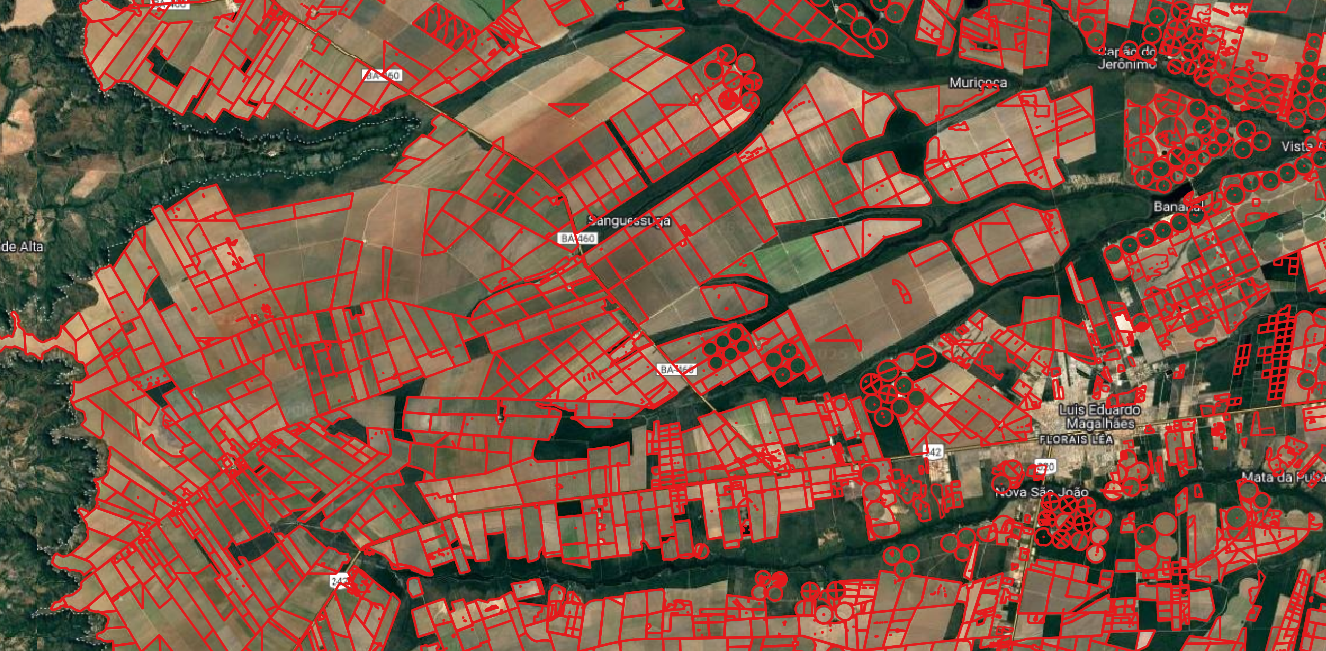
\includegraphics[clip,trim=0.275in 0.55in 0.275in 0.55in,width=1\textwidth]{figures/6_methodology/varda/varda_lem.png}
    \caption{VARDA plots in the municipality of Luis Eduardo Magalhães, Bahia - Brazil.}
    \label{fig:varda_ba}
    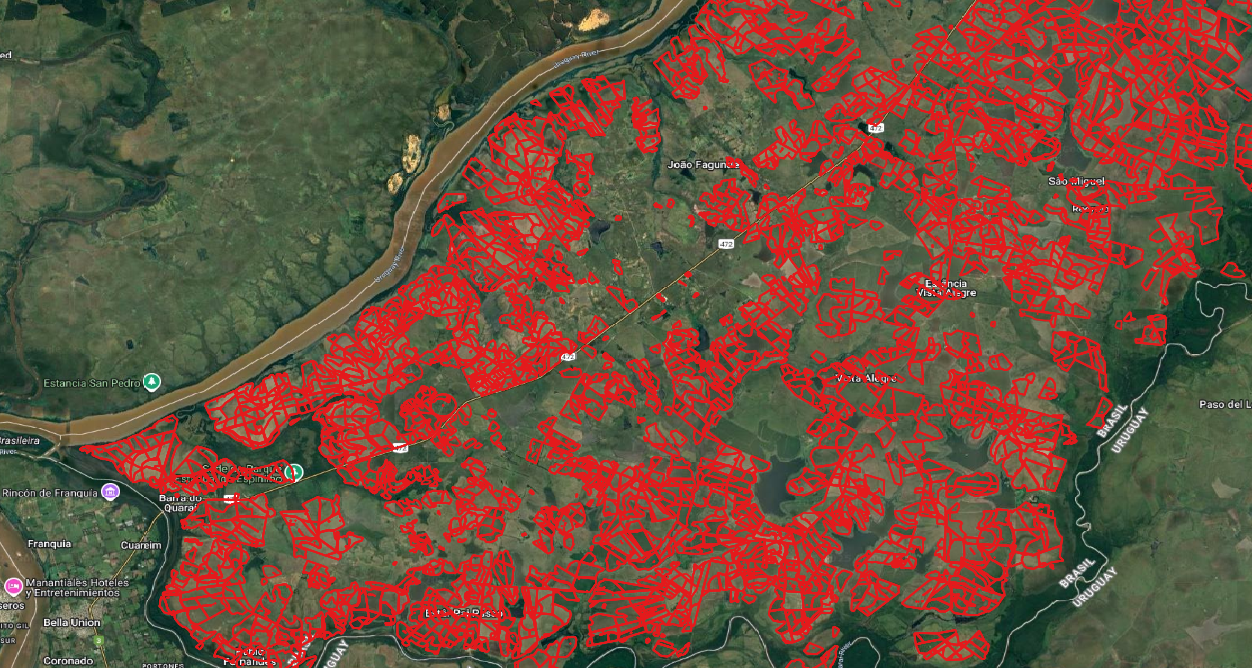
\includegraphics[clip,trim=0.275in 0.55in 0.275in 0.55in,width=1\textwidth]{figures/6_methodology/varda/varda_quarai.png}
    \caption{VARDA plots in the municipality of Barra do Quaraí, Rio Grande do Sul - Brazil.}
    \label{fig:varda_rs}
    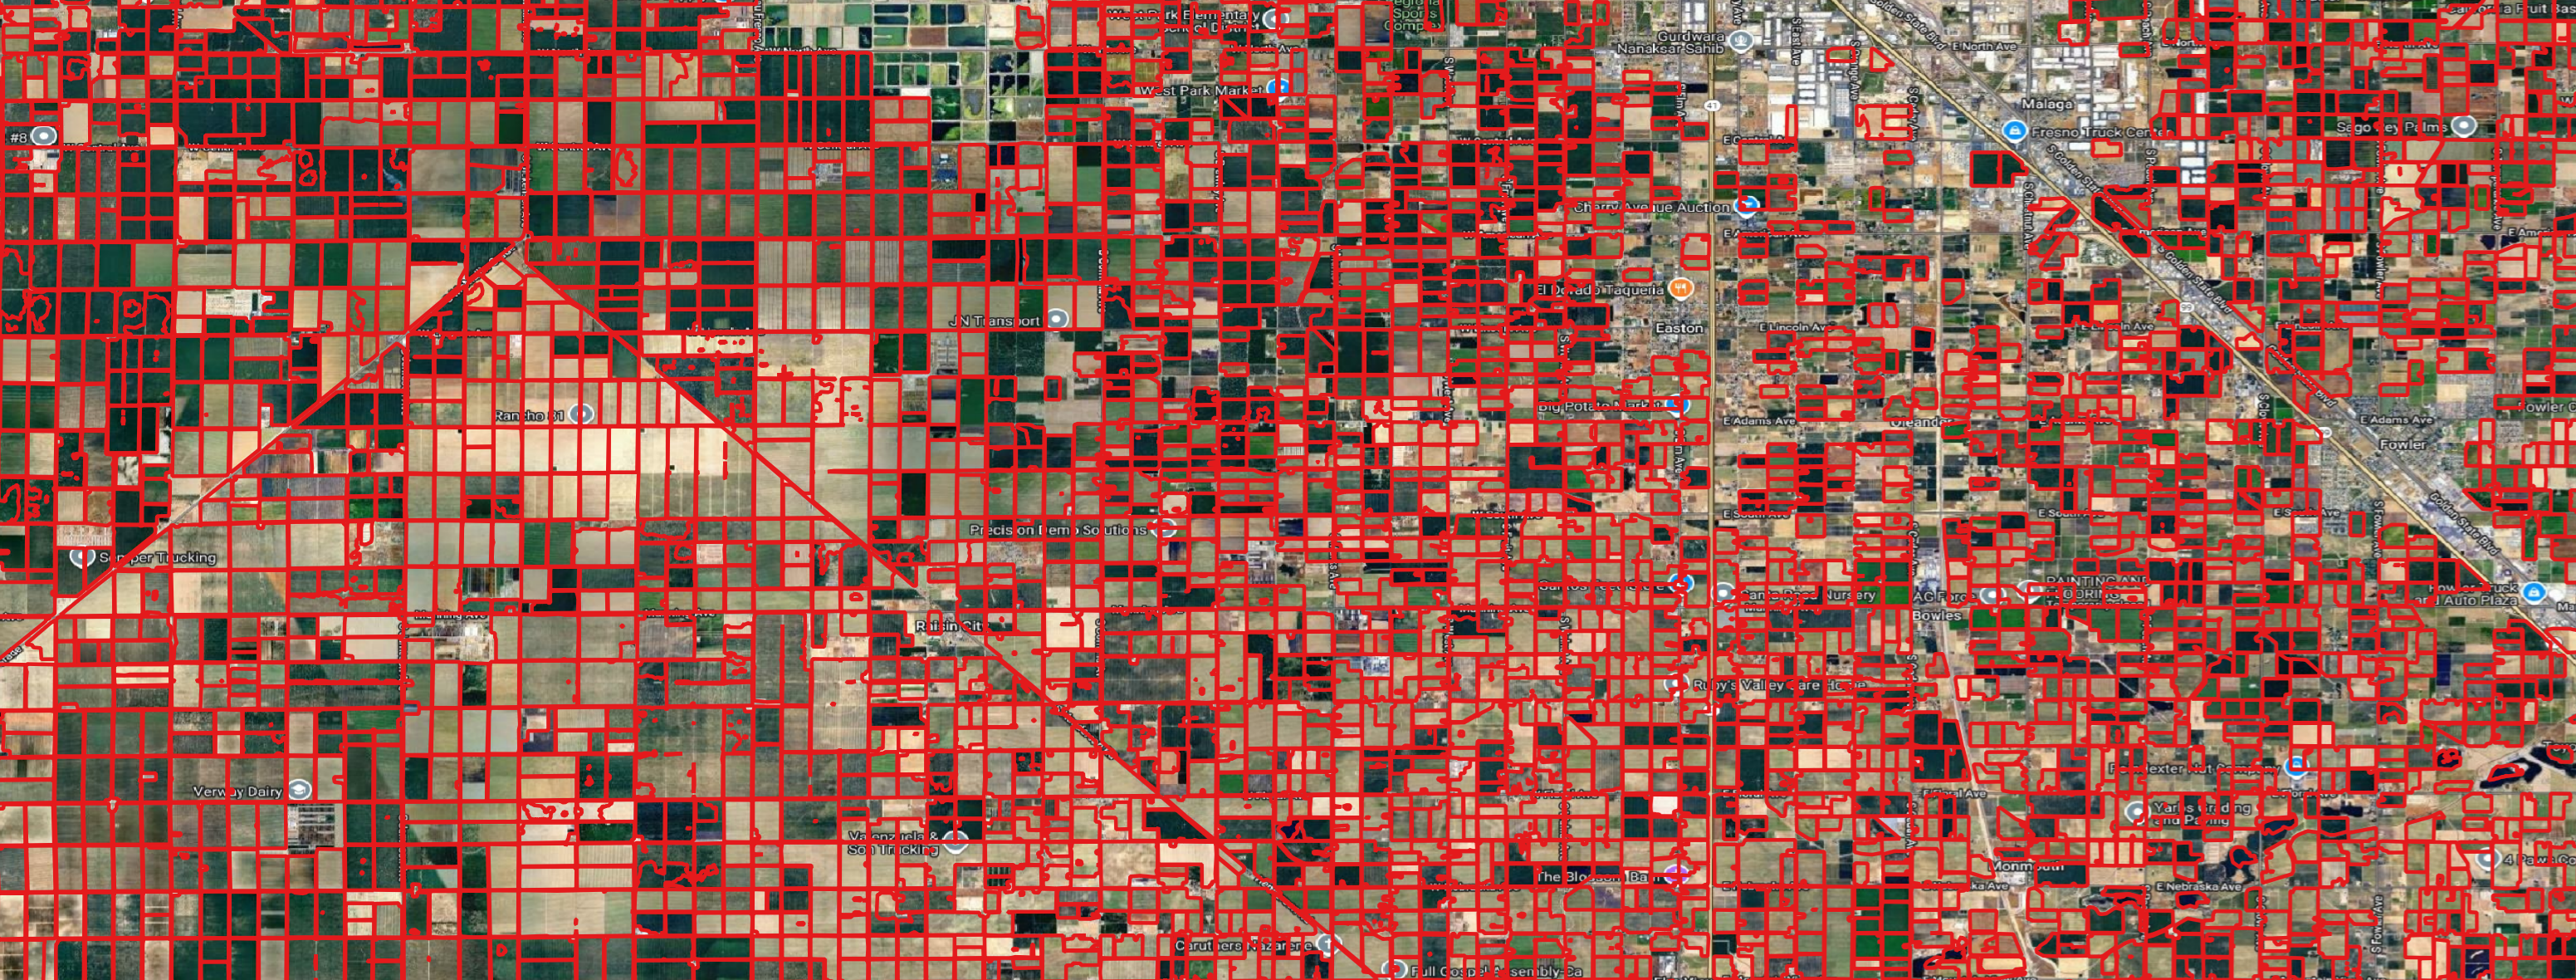
\includegraphics[clip,trim=0.275in 0.55in 0.275in 0.55in,width=1\textwidth]{figures/6_methodology/varda/varda_fresno.png}
    \caption{VARDA plots in the municipality of Fresno, California - USA.}
    \label{fig:varda_fresno}
\end{figure}

The database is updated monthly and contains data from Argentina, Belgium, Brazil, Canada, the Czech Republic, Germany, Denmark, Spain, Estonia, Finland, France, the United Kingdom, India, Italy, Japan, Lithuania, Latvia, the Netherlands, Norway, Poland, Sweden, the United States, and South Africa. In addition to the monthly files, it is possible to obtain data from APIs, which were not used in this study. It is quite noticeable, due to common errors in convolutional models (see Figure \ref{fig:varda_errors}), that most of the plots were generated using \ac{DL} models with the Sentinel 2 MSI sensor, which has a maximum spatial resolution of 10 meters. Access to Global FieldID is free for consultation and download when used in academic research and non-commercial projects.

\begin{figure}[!ht]
    \centering
    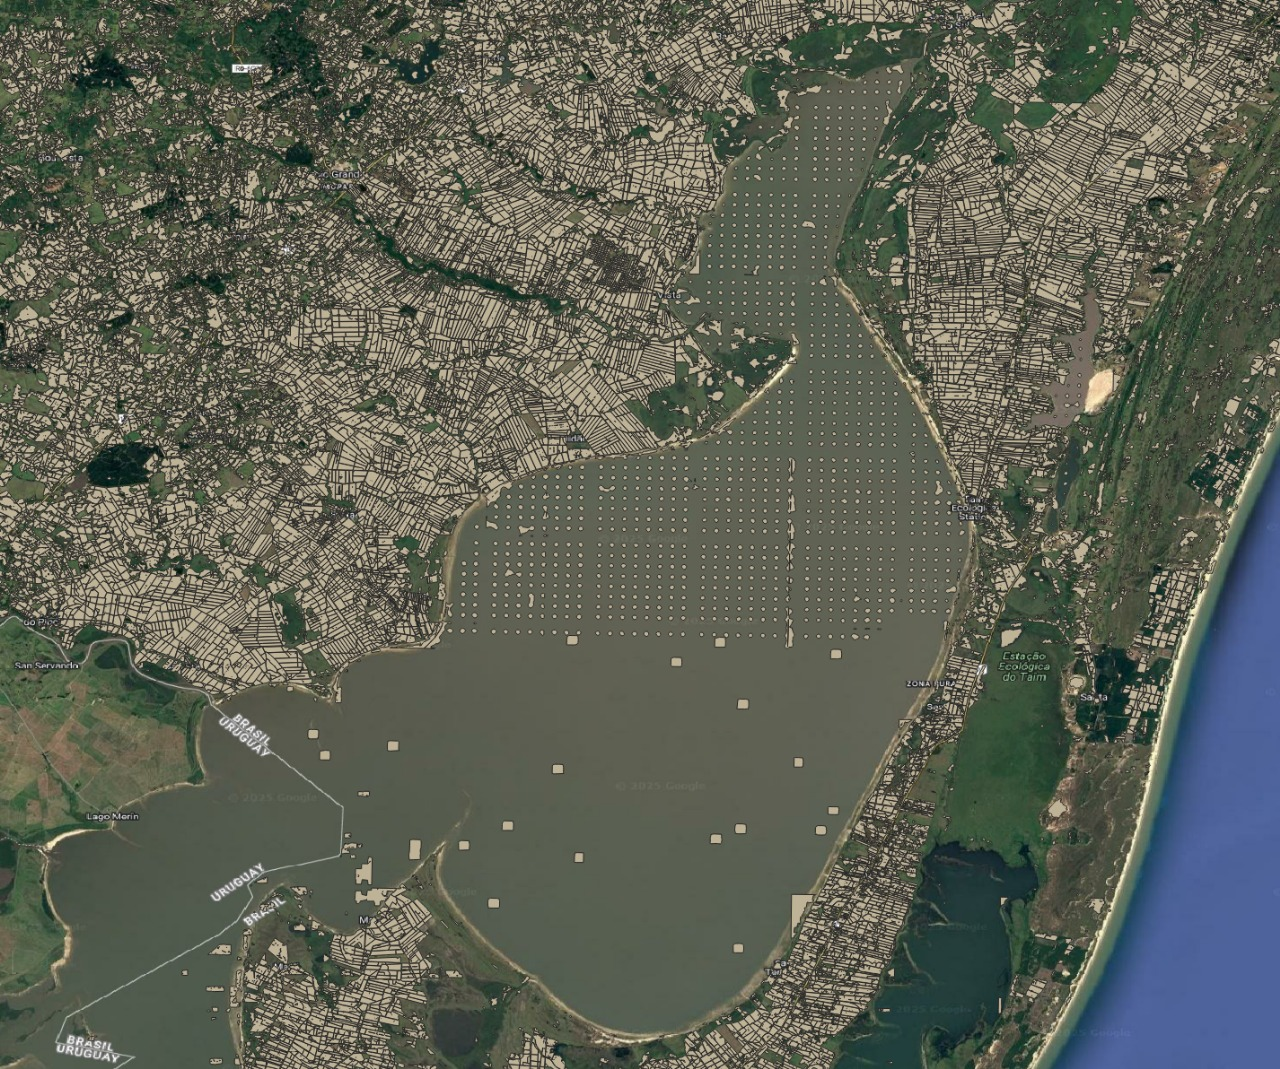
\includegraphics[clip,trim=0.275in 0.55in 0.275in 0.55in,width=1\textwidth]{figures/6_methodology/varda/varda_erros.jpg}
    % }
    \caption{Agricultural plots mistakenly identified in the water in Lagoa dos Patos, in the extreme south of Brazil, on the border between Brazil and Uruguay.}
    \label{fig:varda_errors}
\end{figure}

Parcels smaller than 1 hectare were filtered out, as they are practically just noise in the VARDA dataset. In addition, it is noteworthy that there are many missing parcels, i.e., parcels that exist in reality but are not present in the dataset - especially in regions where parcels are not so well delimited, such as in southern Brazil.

In terms of data quantity, the VARDA dataset is well spread geographically. For Brazil, there is more data for the southeast region and Bahia, but this is in line with the expected number of agricultural parcels across the country (see Figure \ref{fig:varda_qnt}). In California, there are 277,634 parcels, and in Texas, there are 658,018 parcels - all after filtering out parcels smaller than 1 hectare. The main use of Varda Global FieldID in this work is to delineate each agricultural plot geometry, since the databases with agricultural labels (explained below) do not present such information, and may even unify plots that contain the same crop class, for example.

\begin{figure}[!ht]
    \centering
    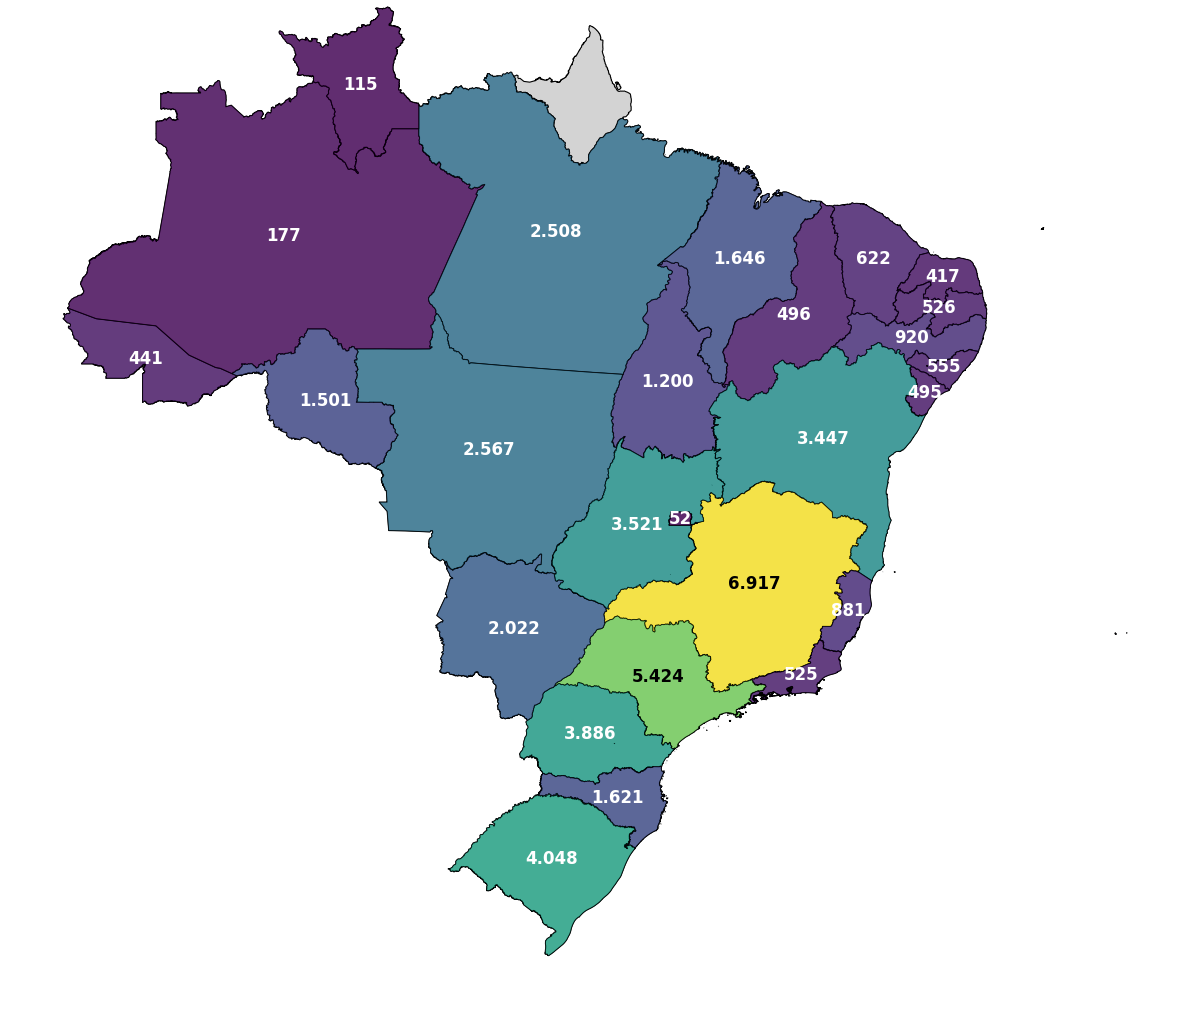
\includegraphics[clip,trim=0.275in 0.55in 0.275in 0.55in,width=0.7\textwidth]{figures/6_methodology/varda/varda_samples_per_uf.png}
    \caption{Number of VARDA parcels in thousands per state in Brazil.}
    \label{fig:varda_qnt}
\end{figure}

\subsection{Mapbiomas Brazil}
\label{sec:mapbiomas}

MapBiomas Brazil \citep{souza2017mapbiomas} is a multi-institutional initiative launched in 2015 by universities, NGOs, and technology companies with the goal of producing annual maps of \ac{LULC} in Brazil at a spatial resolution of 30 meters, covering the historical series from 1985 to the present. The project is organized by biomes (Amazon, Atlantic Forest, Caatinga, Cerrado, Pampa, and Pantanal) and by cross-cutting themes, including Agriculture, Pasture, Forestry, Mining, Coastal Zone, and Urban Area. The methodology is based on the classification of annual mosaics of Landsat images (TM, ETM+, OLI-TIRS sensors), processed on the Google Earth Engine platform. The images undergo cloud/shadow removal and temporal composition optimized for each biome and cross-cutting theme, aiming to maximize spectral contrast between classes. Classification is performed mainly by Random Forest algorithms, one for each year and biome/theme, with training samples collected mainly from stable areas between 1985-2022. For specific agricultural classes and other specific uses, U-Net is also employed.

In the cross-cutting theme of Agriculture, the MapBiomas methodology subdivides the class into temporary and perennial crops, distinguishing up to ten agricultural classes, which are: Citrus, Coffee, Forest Plantation, Palm Oil, Pasture, Other Perennial Crops, Rice, Soybean, Sugar Cane, and Other Temporary Crops (see Figure \ref{fig:mapbiomas}). The detection of these crops involves the use of temporal mosaics per scene, allowing characteristic phenological patterns to be captured.

\begin{figure}[!ht]
    \centering
    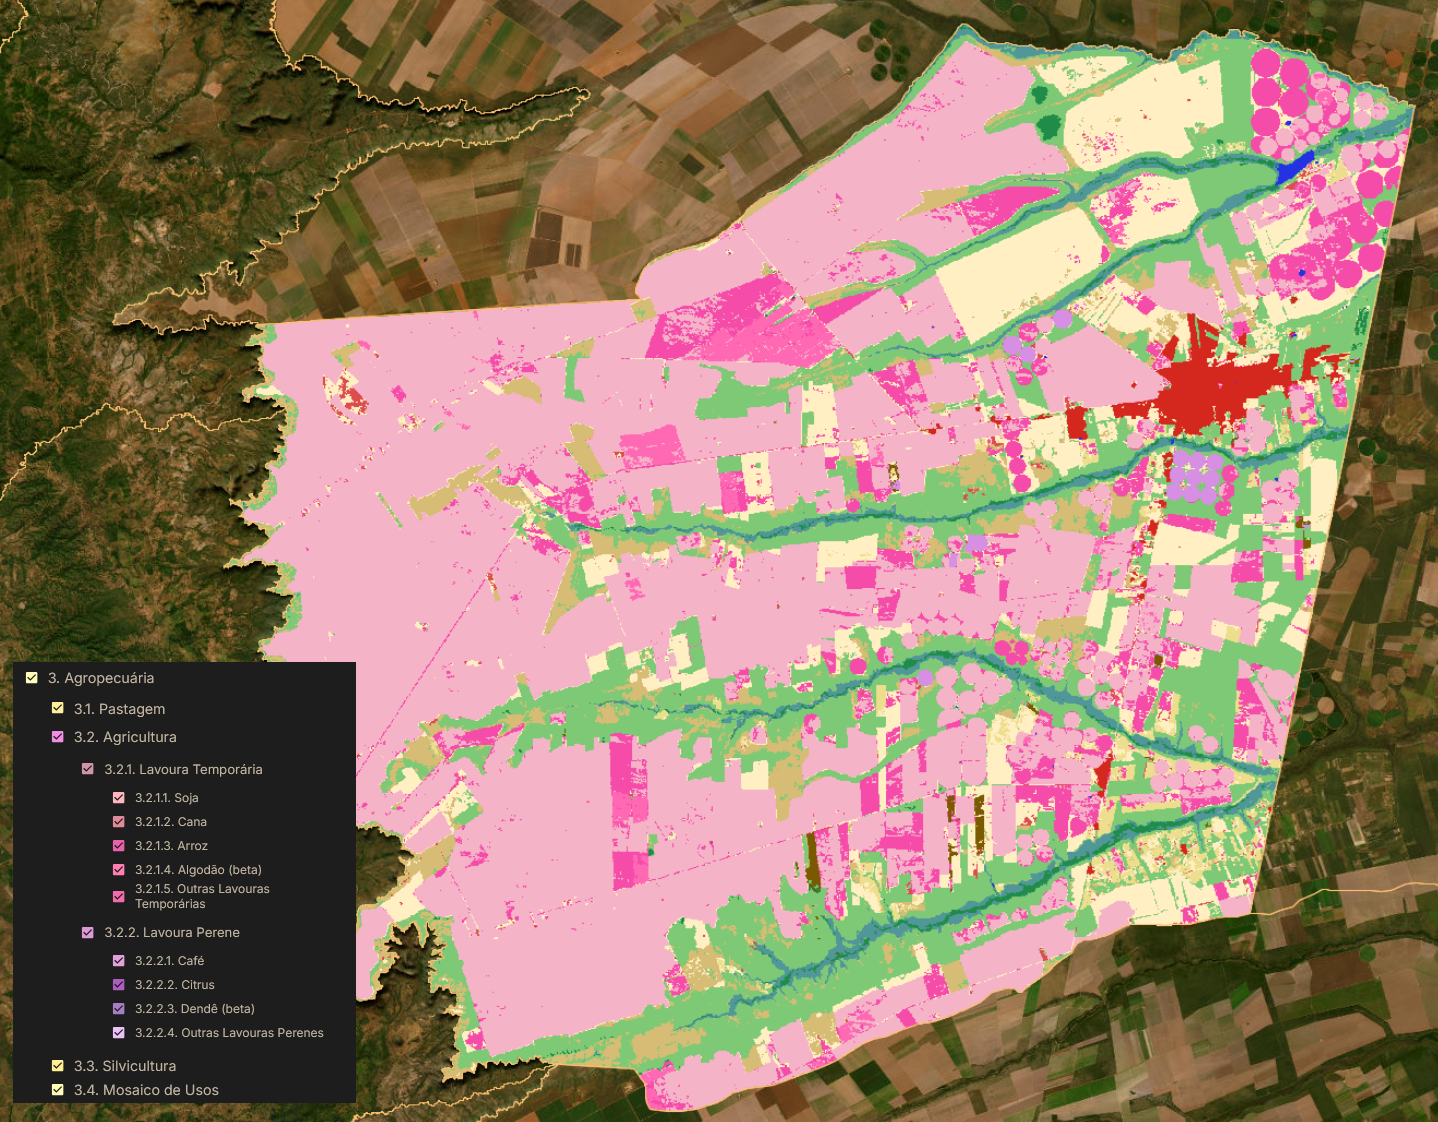
\includegraphics[width=.95\textwidth]{figures/6_methodology/mapbiomas.png}
    \caption{The Mapbiomas 2023 Cropland Raster classification for the city of Luís Eduardo Magalhães, Bahia.}
    \label{fig:mapbiomas}
\end{figure}

Spatial and temporal filters are applied in post-processing to remove noise, correct unrealistic transitions, and stabilize time series. The rules of prevalence between biomes and themes ensure consistency in map integrations. The accuracy assessment of Collection 9 was conducted with approximately 85,000 independent samples per year, for the entire national territory, from 1985 to 2022. Of these, about 10,000 were used for training in the Amazon biome. The validation set, with approximately 75,000 samples/year, was labeled by experts via visual interpretation of Landsat images, MODIS-NDVI series, and high-resolution images. The average overall accuracy for Level 2 of the legend- which contains the classes used for agriculture - was 89.8\%.

However, some details of the Mapbiomas data used in this study are important to highlight. First, Mapbiomas is very clear that its data is LULC and not agricultural land use, which implies that areas classified as agricultural may not actually be in active agricultural use, i.e., an area of temporary crops may mean that temporary crops are normally planted there, but in that specific year it may be fallow or planted with another crop not included in the classification. Therefore, some confusion between certain crops is to be expected, for example between sugarcane and soybeans, as soybean planting is used to regenerate the soil before planting sugarcane, which is a very common crop rotation in Brazil.

The primary use of Mapbiomas Brasil in this work is to extract the labels of the crop classes present in the country. Note that there are other sources of crop class data for Brazil, notably the CONAB maps\footnote{Conab (Companhia Nacional de Abastecimento): \url{https://portaldeinformacoes.conab.gov.br/mapeamentos-agricolas.html}}, but Mapbiomas Brasil, as far as we researched, is the only source with a single map that covers the entire country containing all the main agricultural crops.

\subsection{USDA Cropland Raster}
\label{sec:usda}

The Cropland Data Layer (CDL) is an annual, georeferenced raster product specific to agricultural crops produced by the National Agricultural Statistics Service (NASS) of the \ac{USDA} (see Figure \ref{fig:usda}). The program, which began in 1997 and expanded its coverage to the entire continental United States in 2008, uses satellite imagery and ground truth data to map agricultural land use and cover.

\begin{figure}[!ht]
    \centering
    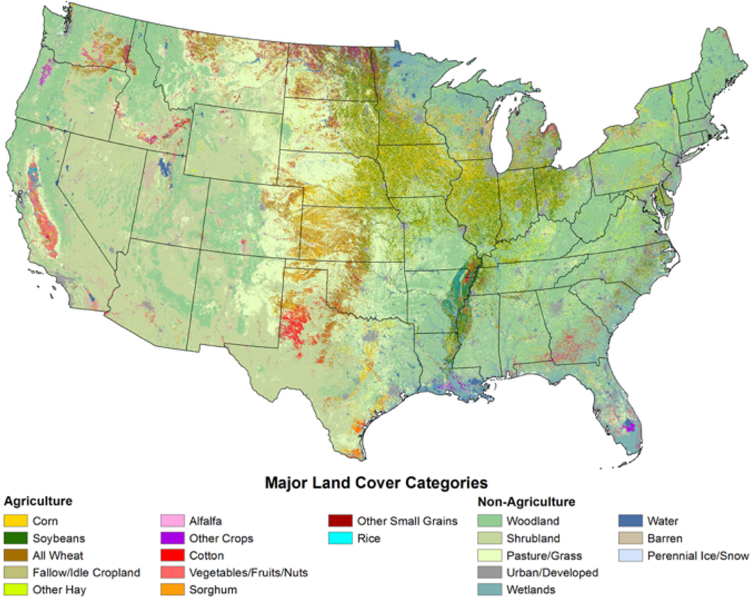
\includegraphics[width=.95\textwidth]{figures/6_methodology/USDA.png}
    \caption{The USDA Cropland Raster.}
    \label{fig:usda}
\end{figure}

Recently, for the 2024 crop year, the program underwent a methodological update, increasing the spatial resolution to 10 meters and migrating the processing flow to the GEE, using \ac{RF}. Previously (2008-2023), the resolution was 30 meters and mostly used \ac{DT}, although we used the 30 meter spatial resolution because we also used data prior to 2023.

The current methodology integrates optical images from OLI/TIRS (Landsat 8 and 9) and MSI (Sentinel-2A and 2B) sensors, harmonized and composited into 10-day medians to reduce cloud cover. In addition to the visible, NIR, SWIR, and RedEdge bands, auxiliary data such as the USGS 3DEP Digital Elevation Model and the official US LULC product, the National Land Cover Database (NLCD), are used.

The strength of the CDL lies in the quality of its training data. For agricultural classes, the model is trained with data from the Farm Service Agency (FSA) Common Land Unit (CLU). The CLU consists of administrative data reported directly by farmers participating in government programs, providing robust and detailed ground truth. For non-agricultural classes, NLCD data is used as a reference. The CDL distinguishes more than 100 land cover categories, focusing on major commodities (such as corn, soybeans, wheat, and cotton) and specialty crops (such as almonds, walnuts, and citrus).

Product accuracy is assessed annually using independent validation sets derived from the FSA CLU. For the 2024 product, producer accuracy for major commodity categories is generally between 85\% and 95\%. The primary use of USDA Cropland Raster in this work is the same as Mapbiomas Brasil, but for US datasets: to remove the labels of the crop classes present in the country.

\section{Pipeline for creating parcel-level crop classification datasets}\label{sec:dataset_creation}

The Figure \ref{fig:meth_datasets} presents the proposed pipeline for creating crop classification datasets at the plot level. The method integrates agricultural plot design data with Cropland Rasters, using Google Earth Engine (GEE) for cloud processing and statistical filtering based on agricultural spectral indices.

\begin{figure}[ht!]
    \centering
    \caption{Graphical abstract showing the pipeline for creating parcel-level crop classification dataset.}
    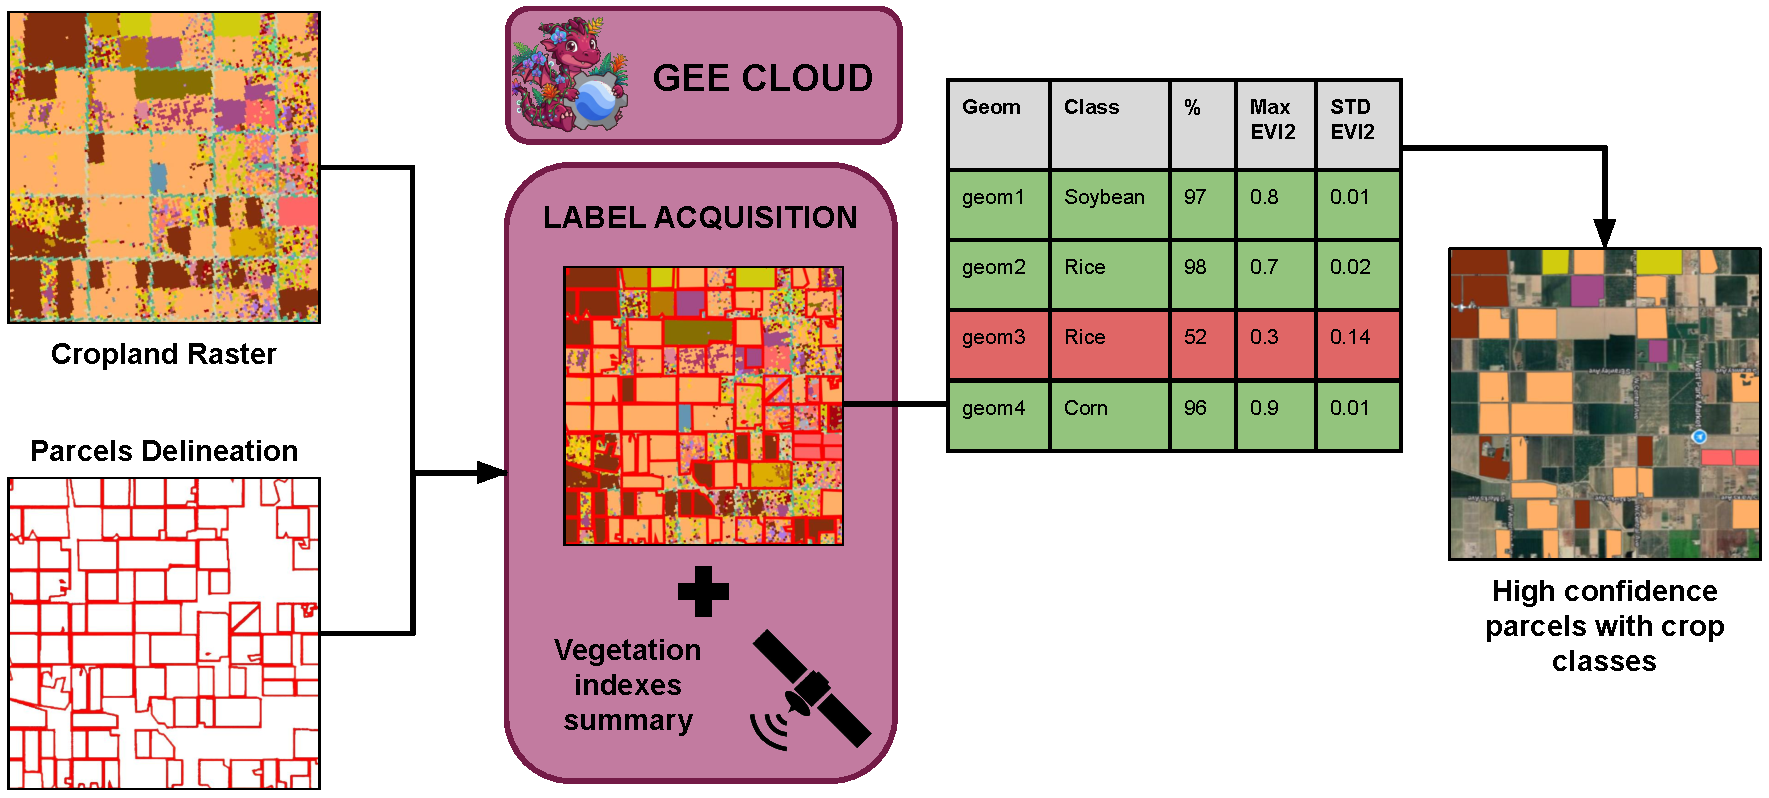
\includegraphics[width=.95\linewidth]{figures/6_methodology/creating_datasets.pdf}
    \label{fig:meth_datasets}
\end{figure}

First, basic descriptive statistics for each geometry are extracted. The crop class of a plot is determined by the most frequent label within that polygon in the corresponding year. To support the subsequent filtering step, the necessary vegetation indices are calculated via GEE Cloud, allowing verification of the plot's agronomic viability.

After that, a filtering step is applied to discard malformed or inconsistent parcels. This process imposes the following exclusion criteria:

\begin{itemize}
\item \textbf{Label Consistency:} It is verified that the dominant crop class in the parcel corresponds to at least 90\% of its pixels. Plots with excessive mixing of classes (as illustrated by \textbf{geom3} in the table in Figure \ref{fig:meth_datasets}) are removed.
\item \textbf{Confidence and Cultivation:} It is ensured that the average confidence of the class pixels is greater than  and that, using the binary cultivation channels, at least 90\% of the pixels are marked as cultivated, if this information exists in the Cropland Raster.
\item \textbf{Agricultural Filter (EVI2):} An agricultural filter was incorporated to eliminate geometries that were not effectively cultivated. Using GEE, the timestamp with the highest \ac{EVI2} is identified, corresponding to the vegetative peak. Samples with a maximum median EVI2 of less than 0.2 or with a spatial standard deviation greater than 0.2 are discarded to remove, respectively, non-agricultural samples or poorly cut parcels.
\end{itemize}

The final result of this pipeline (right side of Figure \ref{fig:meth_datasets}) is a consolidated set of high confidence agricultural parcels, containing only well-delimited geometries with consistent labels, ready for model fine-tuning.

\section{Lightweight SITS download strategy}
\label{sec:lit_pipe}

Figure \ref{fig:meth_download} illustrates the data acquisition flow, designed to operate entirely on Google Earth Engine (GEE) Cloud through the AgriGEE.lite library we developed (which will be better explained in Section \ref{sec:agl}). This approach converts raw and noisy images into treated and statistically representative time series (Treated Resulting \ac{SITS}). The process is divided into four sequential steps described below:

\begin{figure}[ht!]
    \centering
    \caption{Graphical abstract showing the Lightweight SITS download strategy.}
    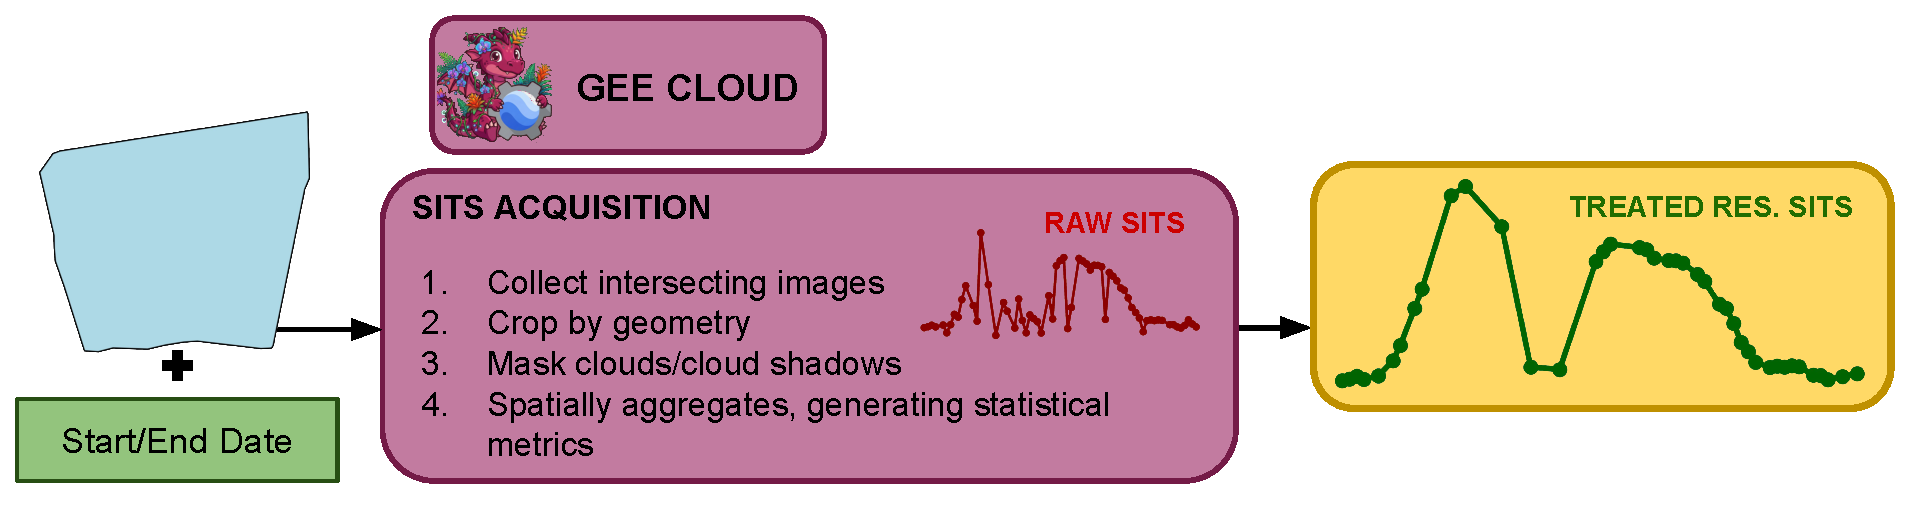
\includegraphics[width=.95\linewidth]{figures/6_methodology/ligthweight_dowload.pdf}
    \label{fig:meth_download}
\end{figure}

\textbf{1. Collect intersecting images} The first step consists of consulting the satellite image catalog, using the corresponding start and end dates. Although the methodology is sensor-agnostic, this work uses Sentinel-2 surface reflectance data, collecting all available scenes that spatially intersect the input geometry.

\textbf{2. Crop by geometry} To ensure that only the area of interest is processed, the collected images are clipped using the parcel outline. 

\textbf{3. Mask clouds/cloud shadows} The third step applies a quality filter. For Sentinel 2, the Cloud Score+ S2 mask is used to remove pixels with a cloud probability greater than 70\%. The pipeline preserves a timestamp as long as at least 20 pixels remain free of clouds or shadows in the parcel. This maximizes the temporal density of the series, recovering information on partially cloudy dates.

\textbf{4. Spatially aggregates, generating statistical metrics} Finally, the pipeline performs spatial aggregation of the remaining valid pixels. For each date, up to 1,000 pixels are randomly sampled within the cropped geometry, and statistics for each spectral band are calculated; in this study, only the median is used. The choice of the median, rather than the mean, aims to mitigate the influence of extreme residual values coming from flaws in the cloud mask. Furthermore, it is important to note that agriculture tends to be uniform within the plot. The result is a lightweight time series, composed of a pseudo-pixel with a single representative value per band per date, drastically reducing the dimensionality of the data while preserving the phenological spectral signature of the crop.

\section{Texas, California and Brazil datasets}
\label{sec:datasets_overview}

To validate the proposed methodology, three distinct datasets based on \ac{SITS} were developed, covering the entire Brazilian territory and the states of California and Texas in the United States. The Brazilian dataset used  Mapbiomas Brasil rasters for class labels (see Section \ref{sec:mapbiomas}), while the datasets for California and Texas used \ac{USDA} cropland data (see Section \ref{sec:usda}). In all scenarios, the definition of agricultural parcels geometries utilized the parcel delineation from Varda Global FieldID (see Section \ref{sec:varda}). The samples consist of the median of the 10 spectral bands of the Sentinel-2/MSI sensor, processed with the Google Cloud Score+\footnote{Google Cloud Score+: \url{https://developers.google.com/earth-engine/datasets/catalog/GOOGLE_CLOUD_SCORE_PLUS_V1_S2_HARMONIZED}} mask to remove clouds and cloud shadows, ensuring the medians only used spectral information from the crops. The US datasets have been previously introduced by us \citep{pintodasilva2025lightweight}, whereas the Brazilian dataset is a new contribution of this work. However, it is imperative to highlight that the creation and public release of the Texas and California datasets stand as a major standalone contribution of this research to the global remote sensing community. By providing highly curated, parcel-level \ac{SITS} benchmarks for prominent North American agricultural regions, these datasets establish a reliable and open-access foundation for evaluating machine learning models under distinct climatic and phenological conditions. Their publication not only ensures the reproducibility of the proposed pipeline but also actively encourages future studies in domain adaptation, transfer learning, and scalable crop monitoring across diverse geographical contexts.

In terms of temporal coverage and design, the datasets reflect the specific agricultural calendars of their respective regions. The Brazilian dataset covers the years 2022 and 2023, using the local agricultural calendar which begins on October 1 and ends on September 30, with parcel geometries dated January 2025. Conversely, the data from California and Texas span from 2019 to 2023 and follow the calendar year (January 1 to December 31), using parcel geometries from July 2024. The selection of these specific dates for the geometries was strategic, targeting the month corresponding to the predominant vegetative peak in each region to improve edge accuracy. Also, it is important to mention that the historical plot delineations are not maintained by the Varda Global Field ID, or that they prevent geometries from each year from being used.

Although class imbalance is very common in agricultural machine learning and exists in all three datasets, the specific class distributions vary significantly. Figures \ref{fig:bar_brazil}, \ref{fig:bar_california}, and \ref{fig:bar_texas} illustrate the crop counts for Brazil, California, and Texas, respectively. In the Brazilian dataset, it is noteworthy that the most common class is Pasture, with almost twice as many classes as the second largest class, Other Temporary Crops. Furthermore, another notable difficulty is that Pasture, Other Temporary Crops, and Other Perennial Crops are classes that contain more than one Crop Type each, making these classes particularly difficult and possibly noisier. Additionally, because Soybeans and Rice are perennial Crop Classes, some confusion with Other Temporary Crops is expected, while Citrus and Palm Oil are likely to be confused with Other Perennial Crops for the same reason.

\begin{figure}[ht!]
    \centering
    \caption{Crop classes distribution in Brazil SITS dataset.}
    \label{fig:bar_brazil}
    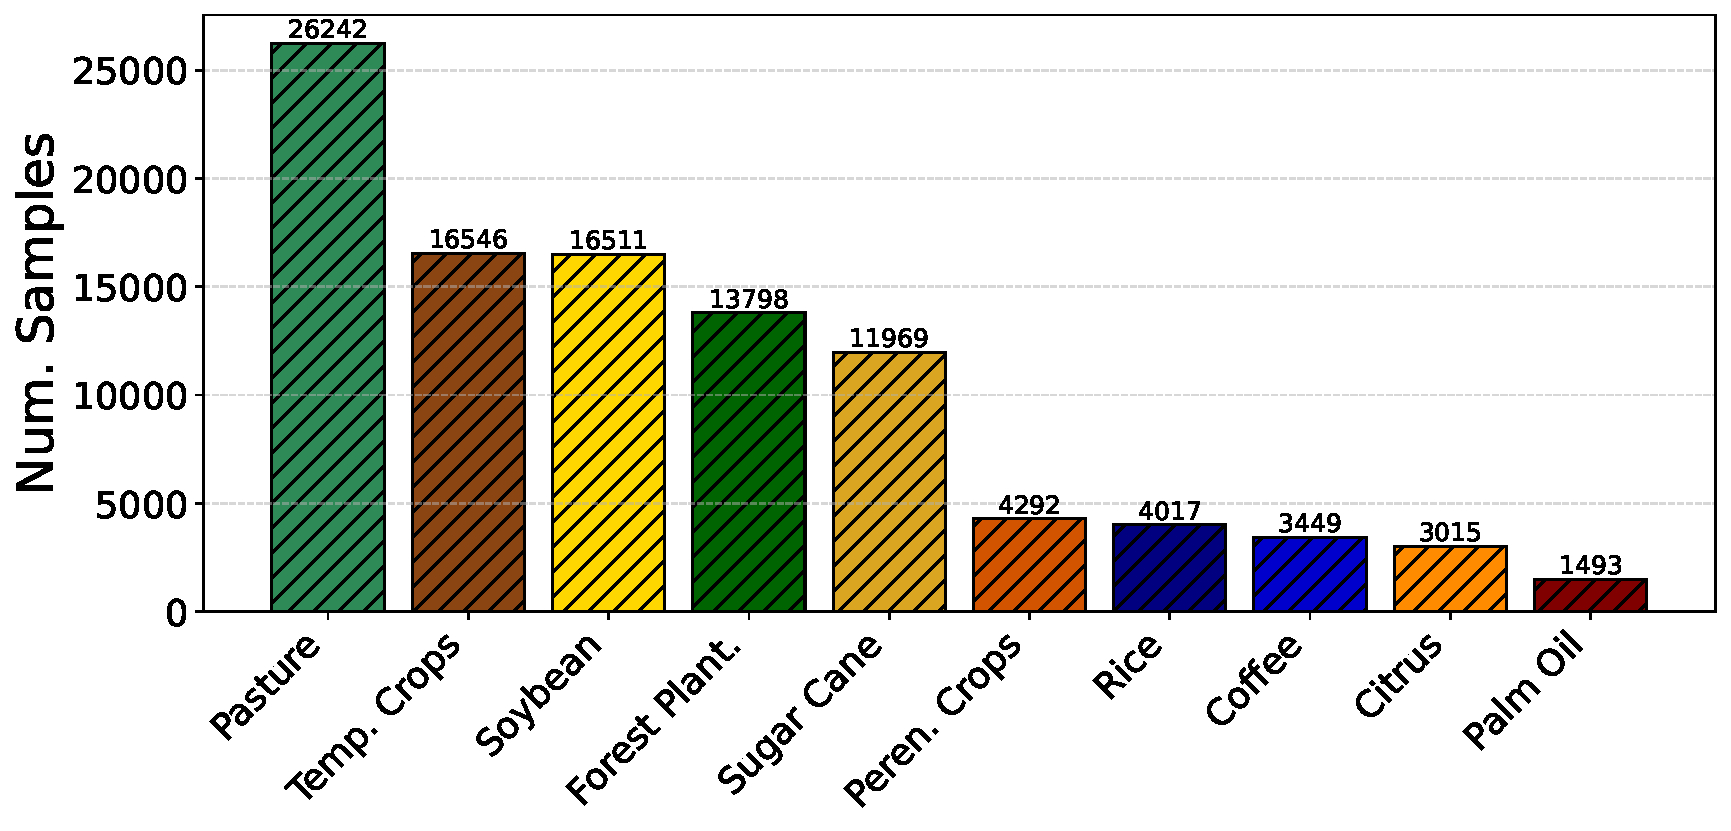
\includegraphics[width=0.6\linewidth]{figures/6_methodology/datasets/brazil_bar_crop.pdf}
\end{figure}

\begin{figure}[ht!]
    \centering
    \caption{Crop classes distribution in California SITS dataset.}
    \label{fig:bar_california}
    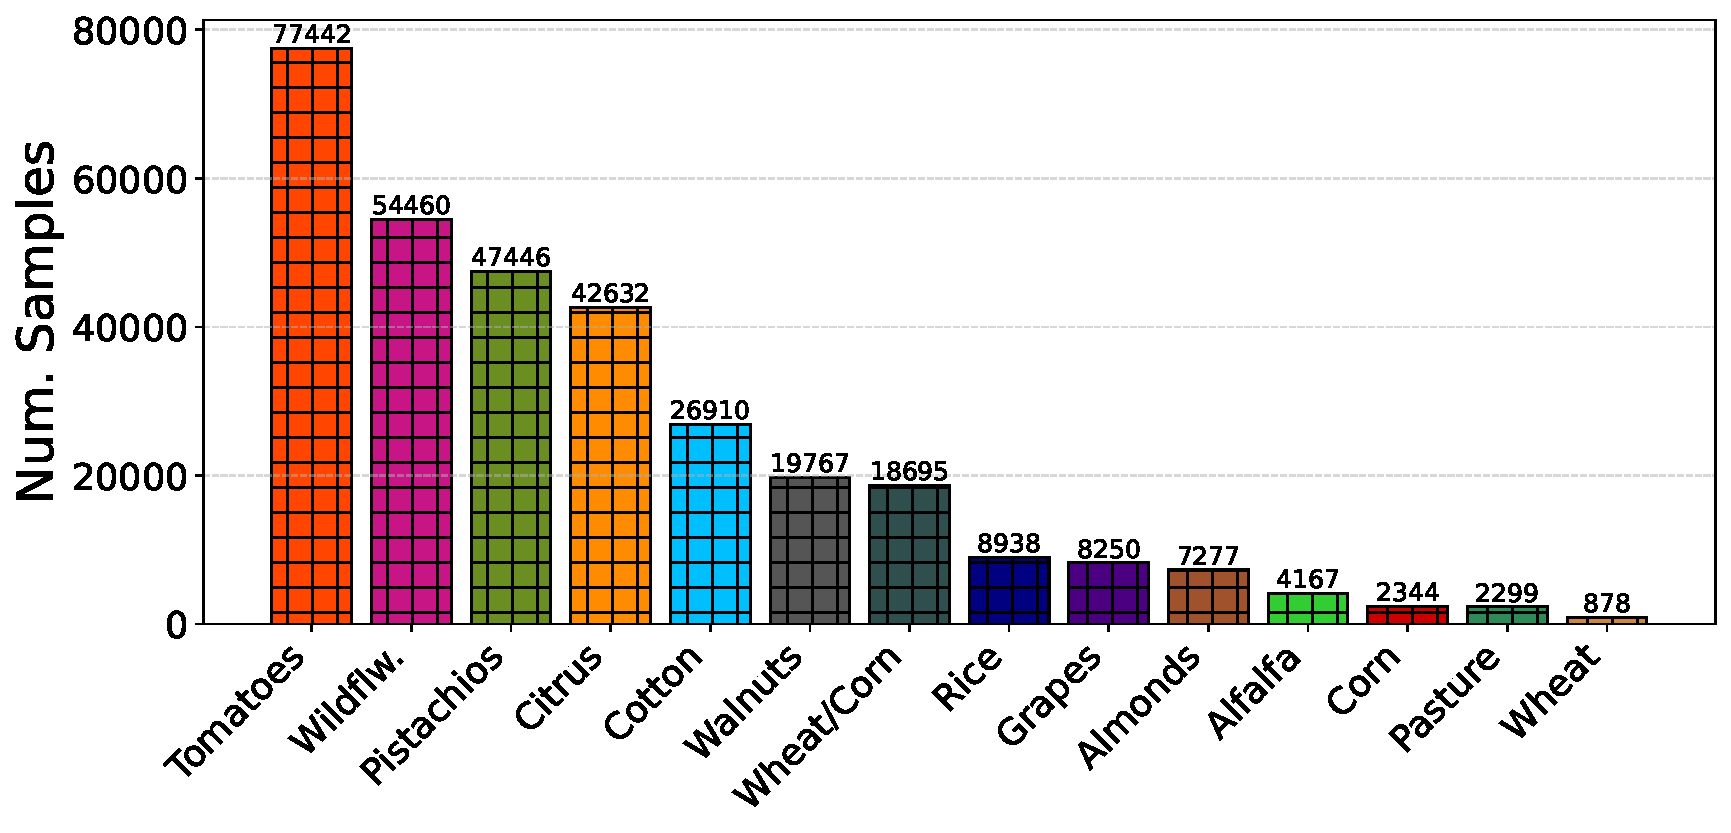
\includegraphics[width=0.6\linewidth]{figures/6_methodology/datasets/california_bar_crop.pdf}
\end{figure}

\begin{figure}[ht!]
    \centering
    \caption{Crop classes distribution in Texas SITS dataset.}
    \label{fig:bar_texas}
        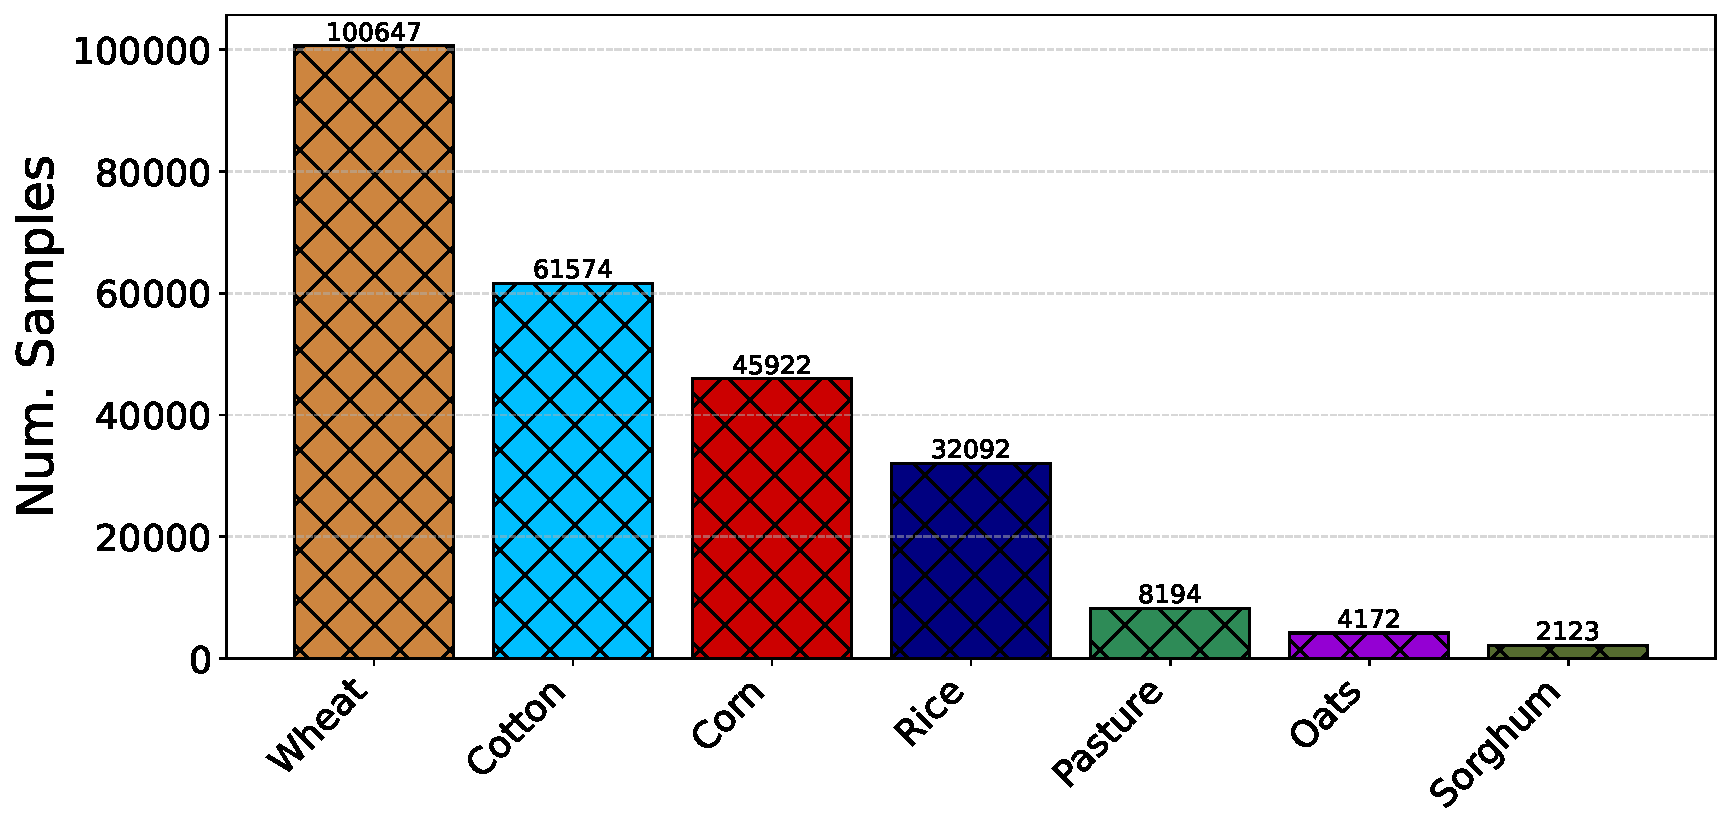
\includegraphics[width=0.6\linewidth]{figures/6_methodology/datasets/texas_bar_crop.pdf}
\end{figure}

Despite the shared challenge of imbalance, the Brazilian dataset is notably more complex than those from California and Texas due to its subcontinental scope and high agricultural variability. As shown in Figure \ref{fig:map_brazil}, the geographical spacing in Brazil leads to distinct regional patterns. For instance, \textit{Soybean} cultivation is heavily concentrated in the Center-West and South, yet planting schedules differ; harvests in the South are generally earlier due to the climate. Other crops, such as \textit{Coffee} and \textit{Sugar Cane}, are clustered in the Southeast, reflecting specific soil and altitude requirements. This heterogeneity requires the model to generalize class features across vastly different biomes. Furthermore, palm oil cultivation is quite geographically localized, as it is planted in degraded areas of the Amazon rainforest. Although the dataset contains plot designs and, consequently, geographic information, this will not be used by the models.

\begin{figure}[ht!]
\centering
\caption{Crop classes regional distribution in Brazil SITS dataset.}
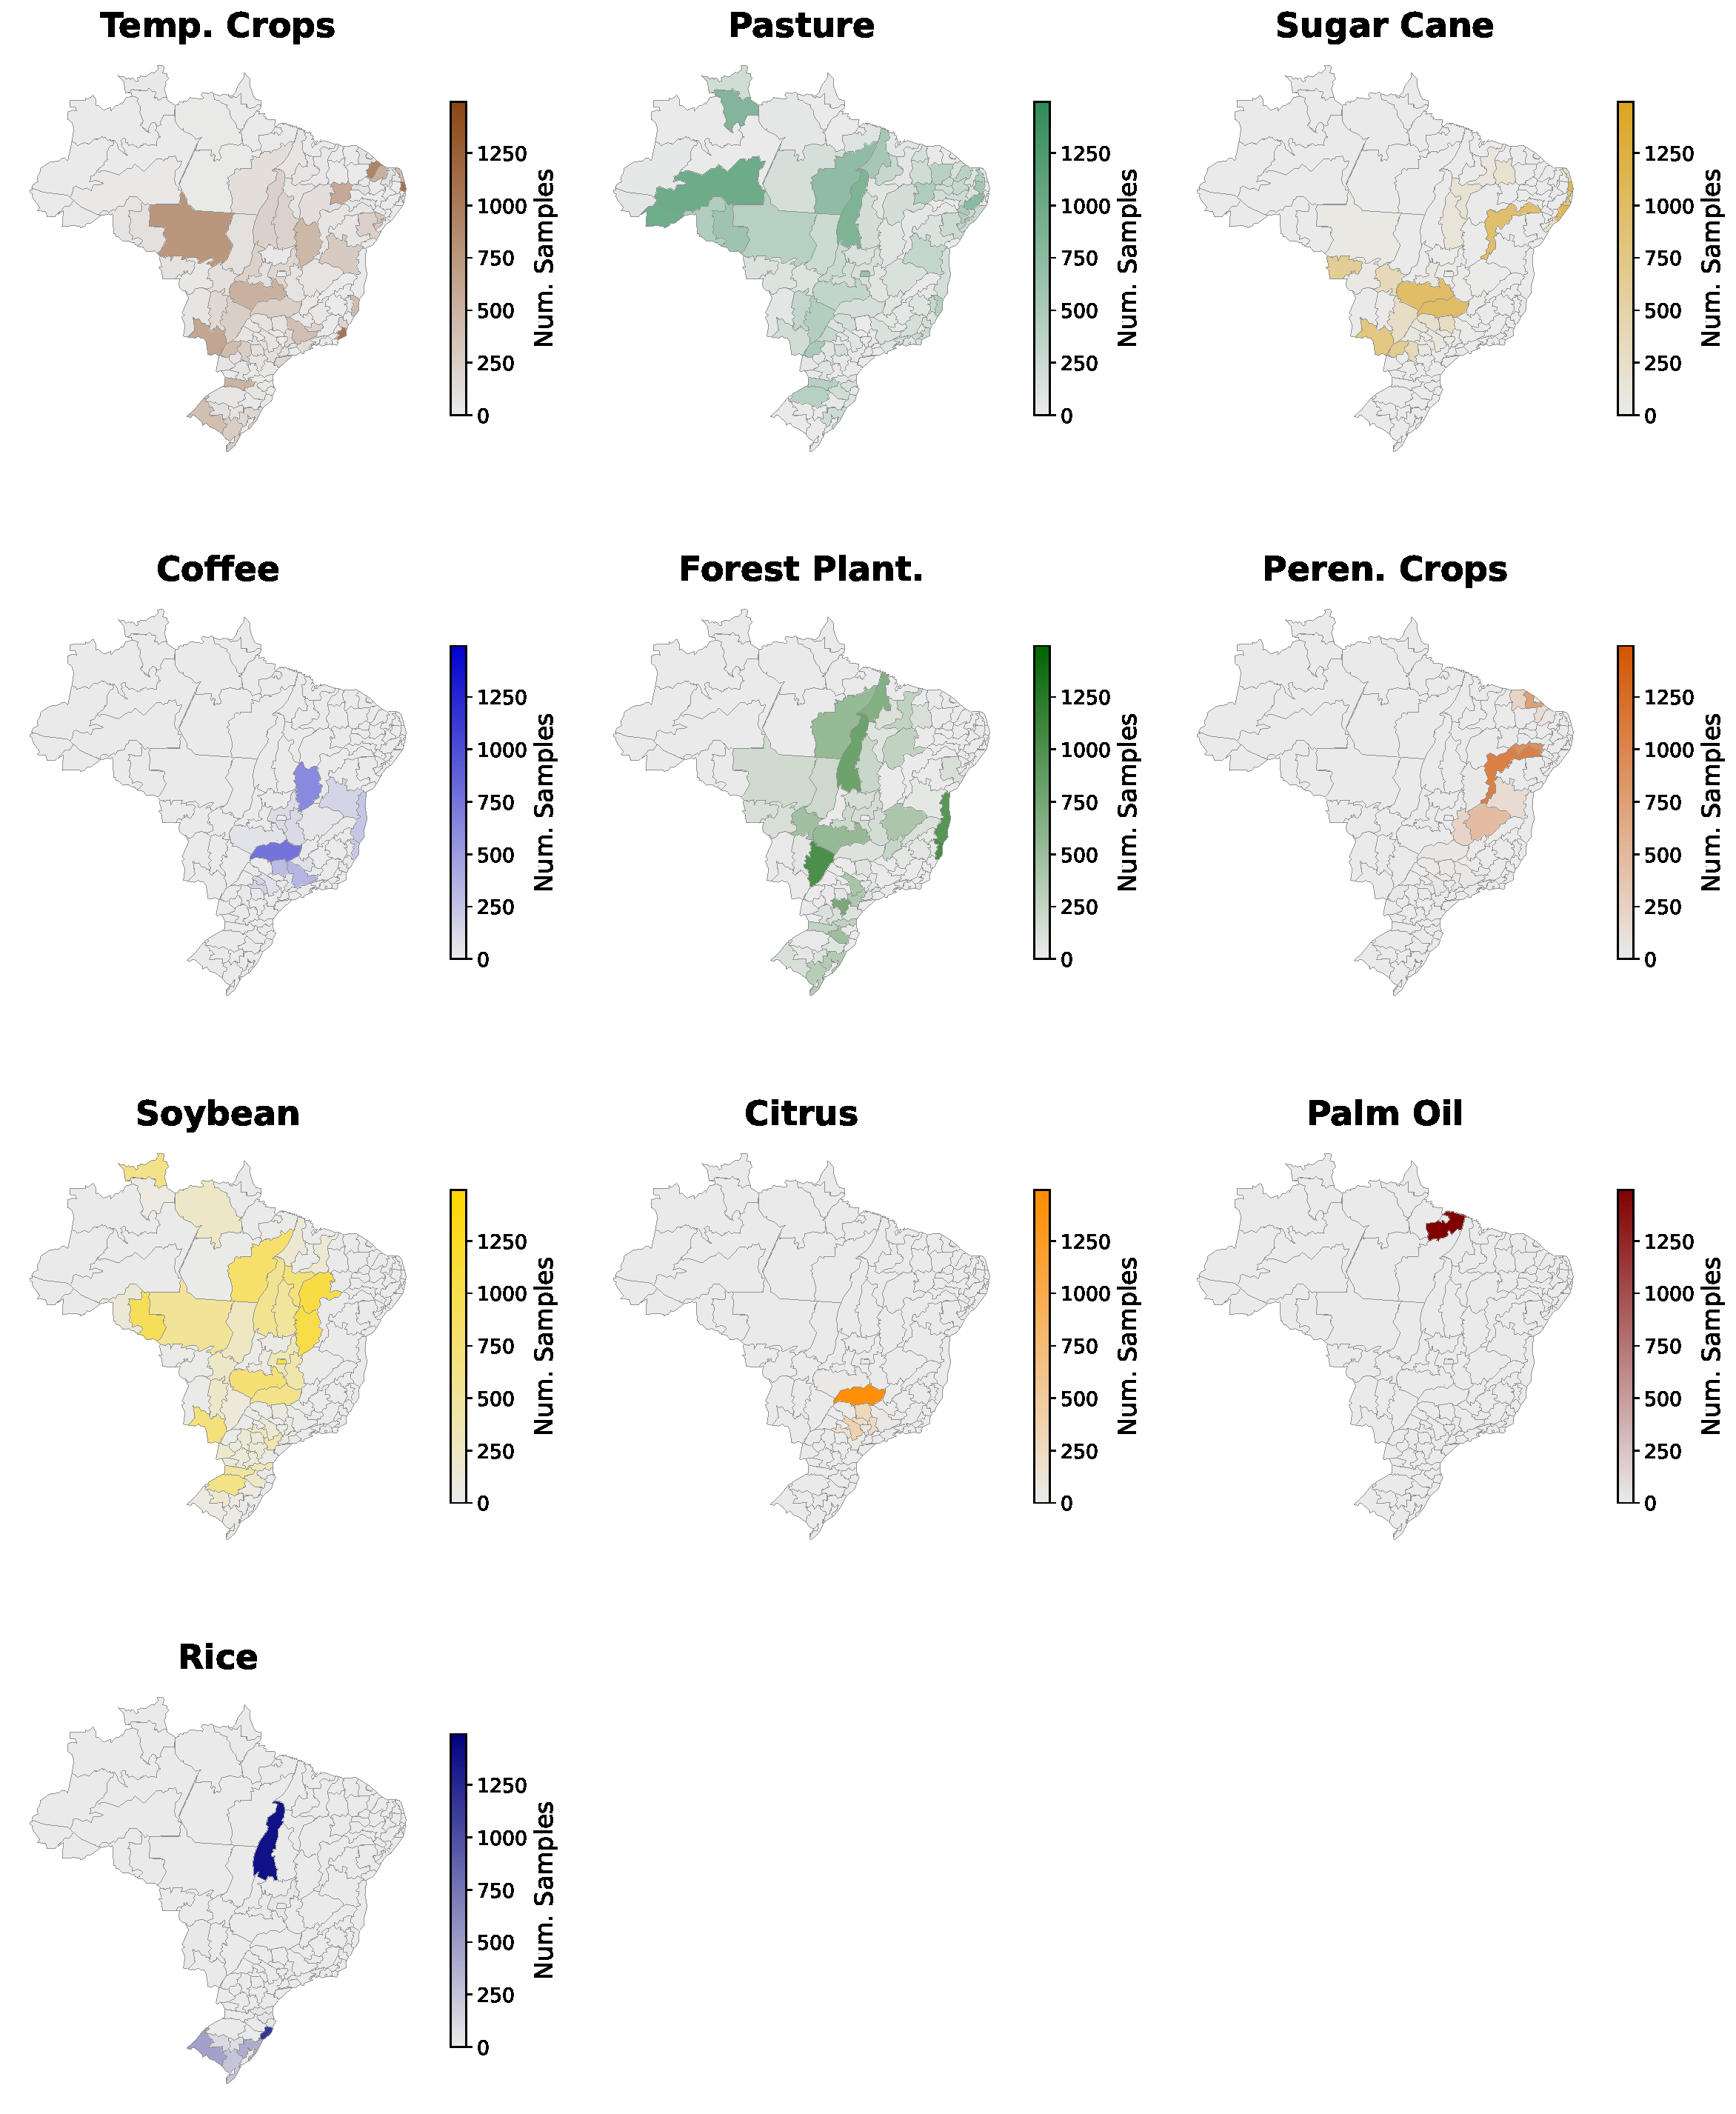
\includegraphics[height=0.7\textheight, keepaspectratio]{figures/6_methodology/datasets/brazil_map_crops.pdf}
\label{fig:map_brazil}
\end{figure}

Furthermore, the phenological behavior of crops in Brazil differs markedly from the US regions. The practice of double cropping (and occasionally triple cropping) in temporary crops is widespread in Brazil. In contrast, agriculture in the US datasets is predominantly single-cycle, with the notable exception of the Wheat/Corn rotation in California. 

This multi-cycle characteristic introduces a specific challenge in the Brazilian dataset: Mapbiomas only provides labels for the primary crop of the year. Consequently, the spectral signals of subsequent crops (often referred to as ``safrinha'') act as noise. This is evident in Figure \ref{fig:evi2_brazil}, where the \textit{Soybean} class exhibits a primary harvest peak followed by secondary EVI2 elevations, likely indicating unregistered corn or cotton. Perennial crops in Brazil, such as \textit{Forest Plantation} and \textit{Citrus}, show stable high EVI2 values, which the model must differentiate from the dynamic peaks of annual crops.

Comparing this to the US datasets, Figure \ref{fig:evi2_california} for California shows the distinct double-peak signature of the labeled \textit{Wheat/Corn} class, while Figure \ref{fig:evi2_texas} for Texas displays clear, single-peak curves for monocultures like \textit{Cotton}, separated by long fallow periods. Furthermore, it is quite evident that the spectral behavior of the crops in both US datasets is much more pronounced and visible in the plots shown, which reinforces that the Brazilian dataset is considerably noisier, inheriting noise from the Mapbiomas Brasil used as a cropland raster.

\begin{figure}[ht!]
\centering
\caption{EVI2 per crop class in Brazil SITS dataset.}
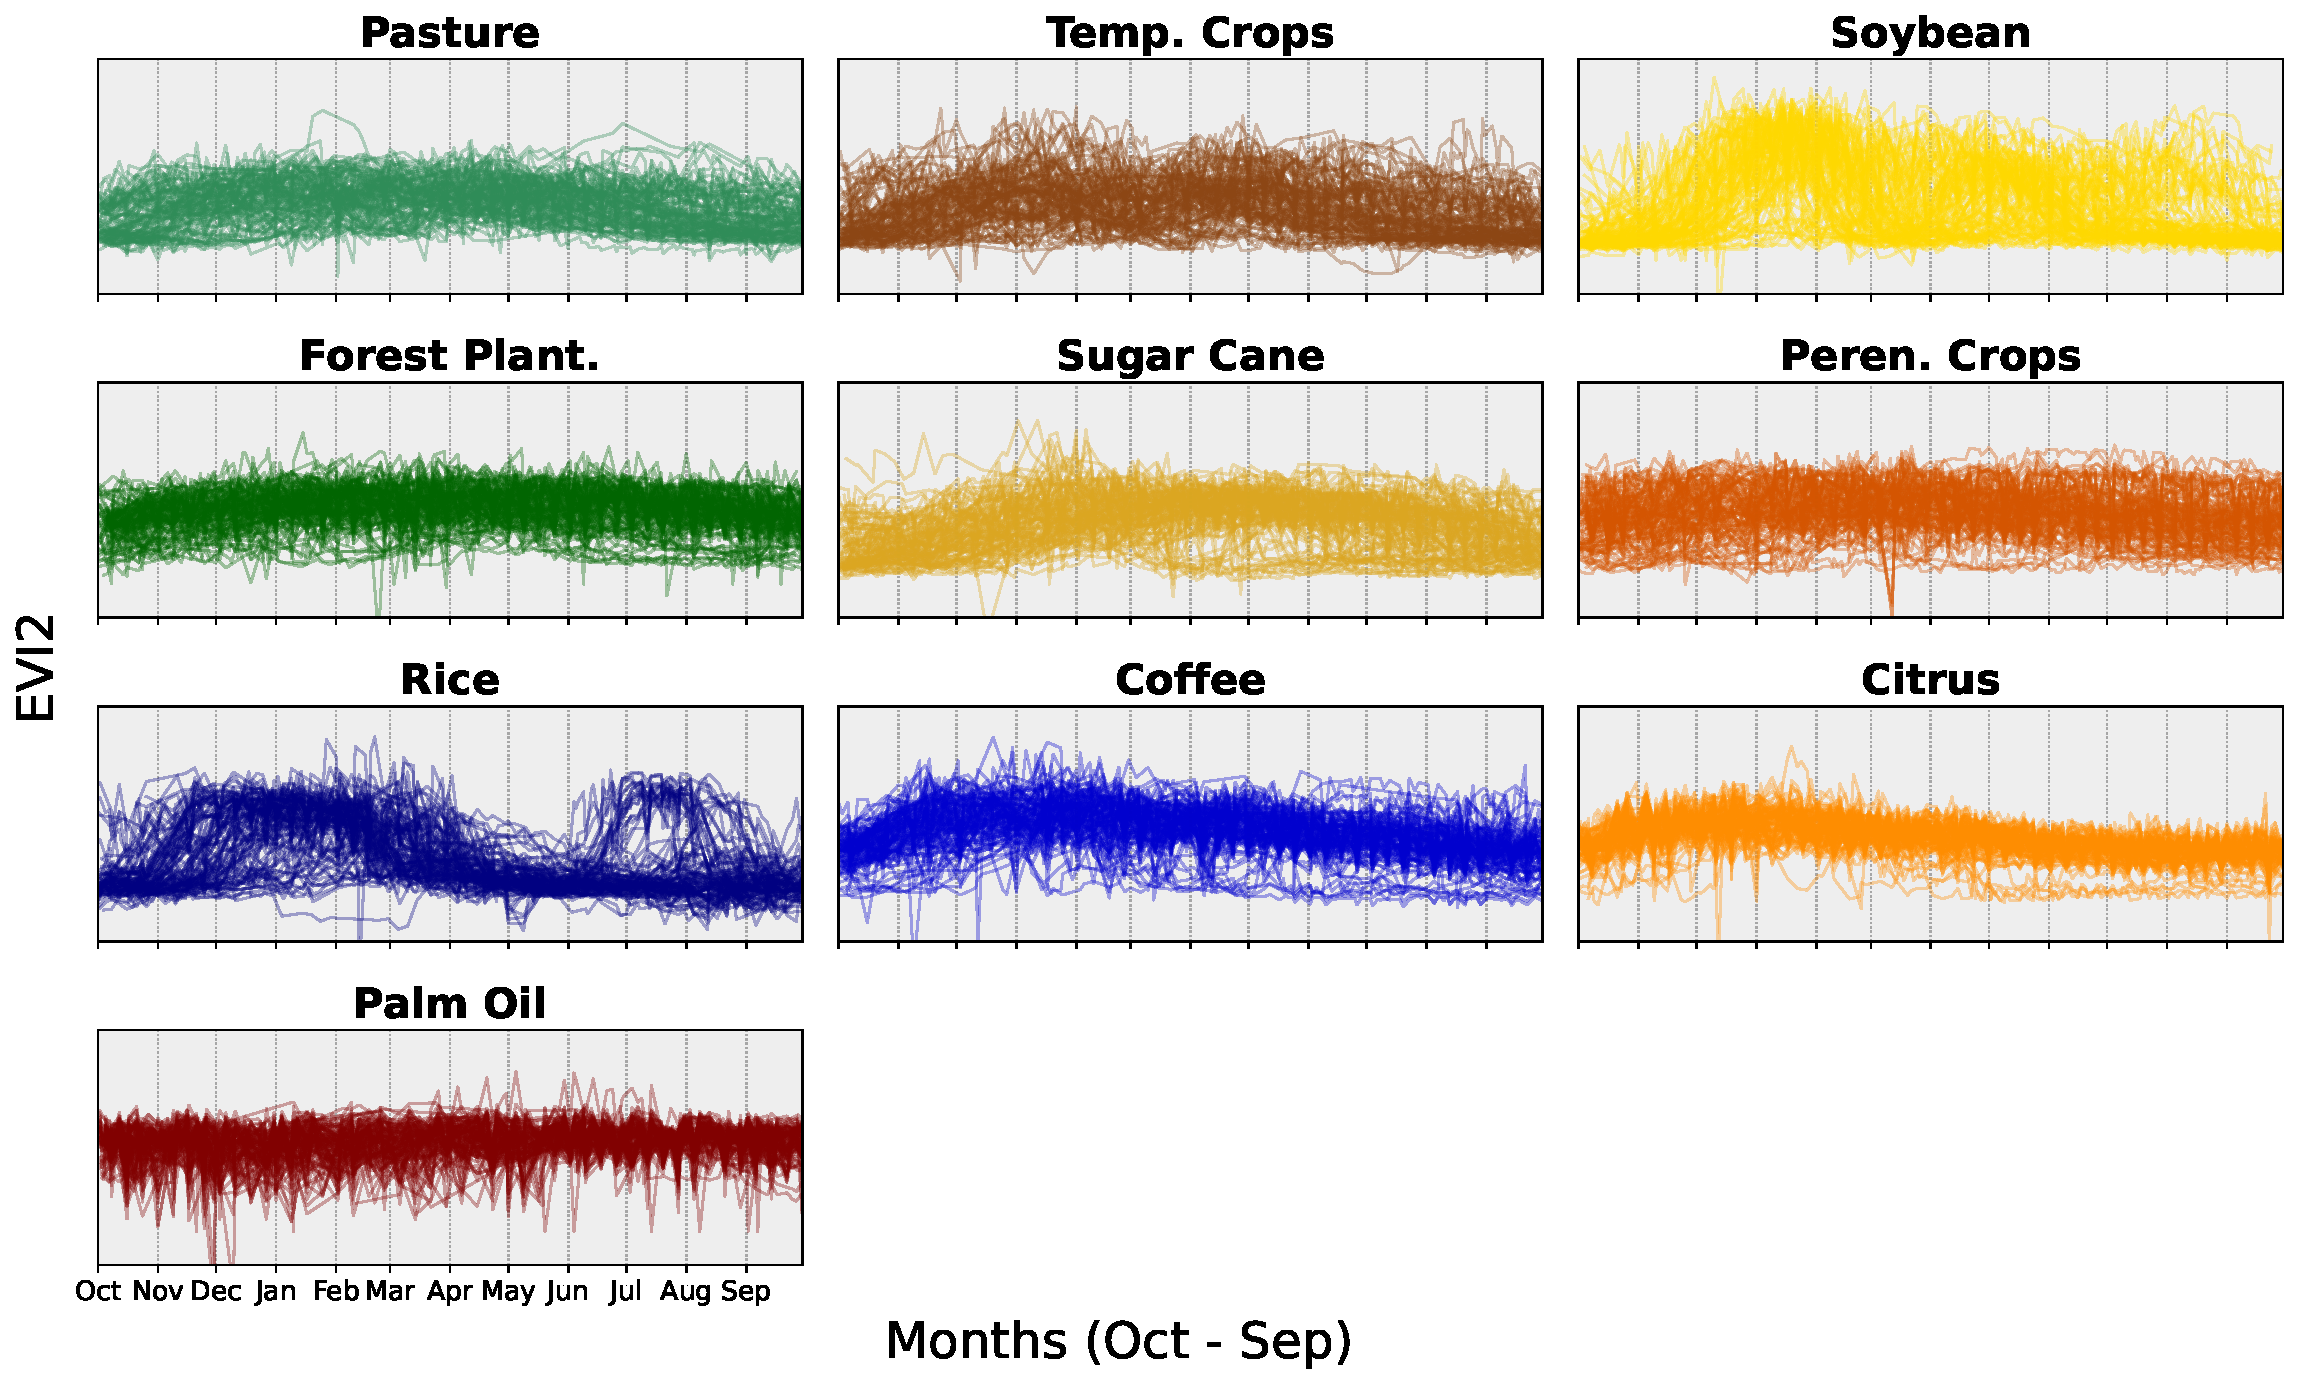
\includegraphics[width=0.7\linewidth]{figures/6_methodology/datasets/brazil_evi2.pdf}
\label{fig:evi2_brazil}
\fignote{Although only EVI2 is shown, which is an agricultural index calculated from Red and NIR and allows for easier visual differentiation of crop classes, the datasets consist of all 10 bands of Sentinel-2.}
\end{figure}

\begin{figure}[ht!]
\centering
\caption{EVI2 per crop class in California SITS dataset.}
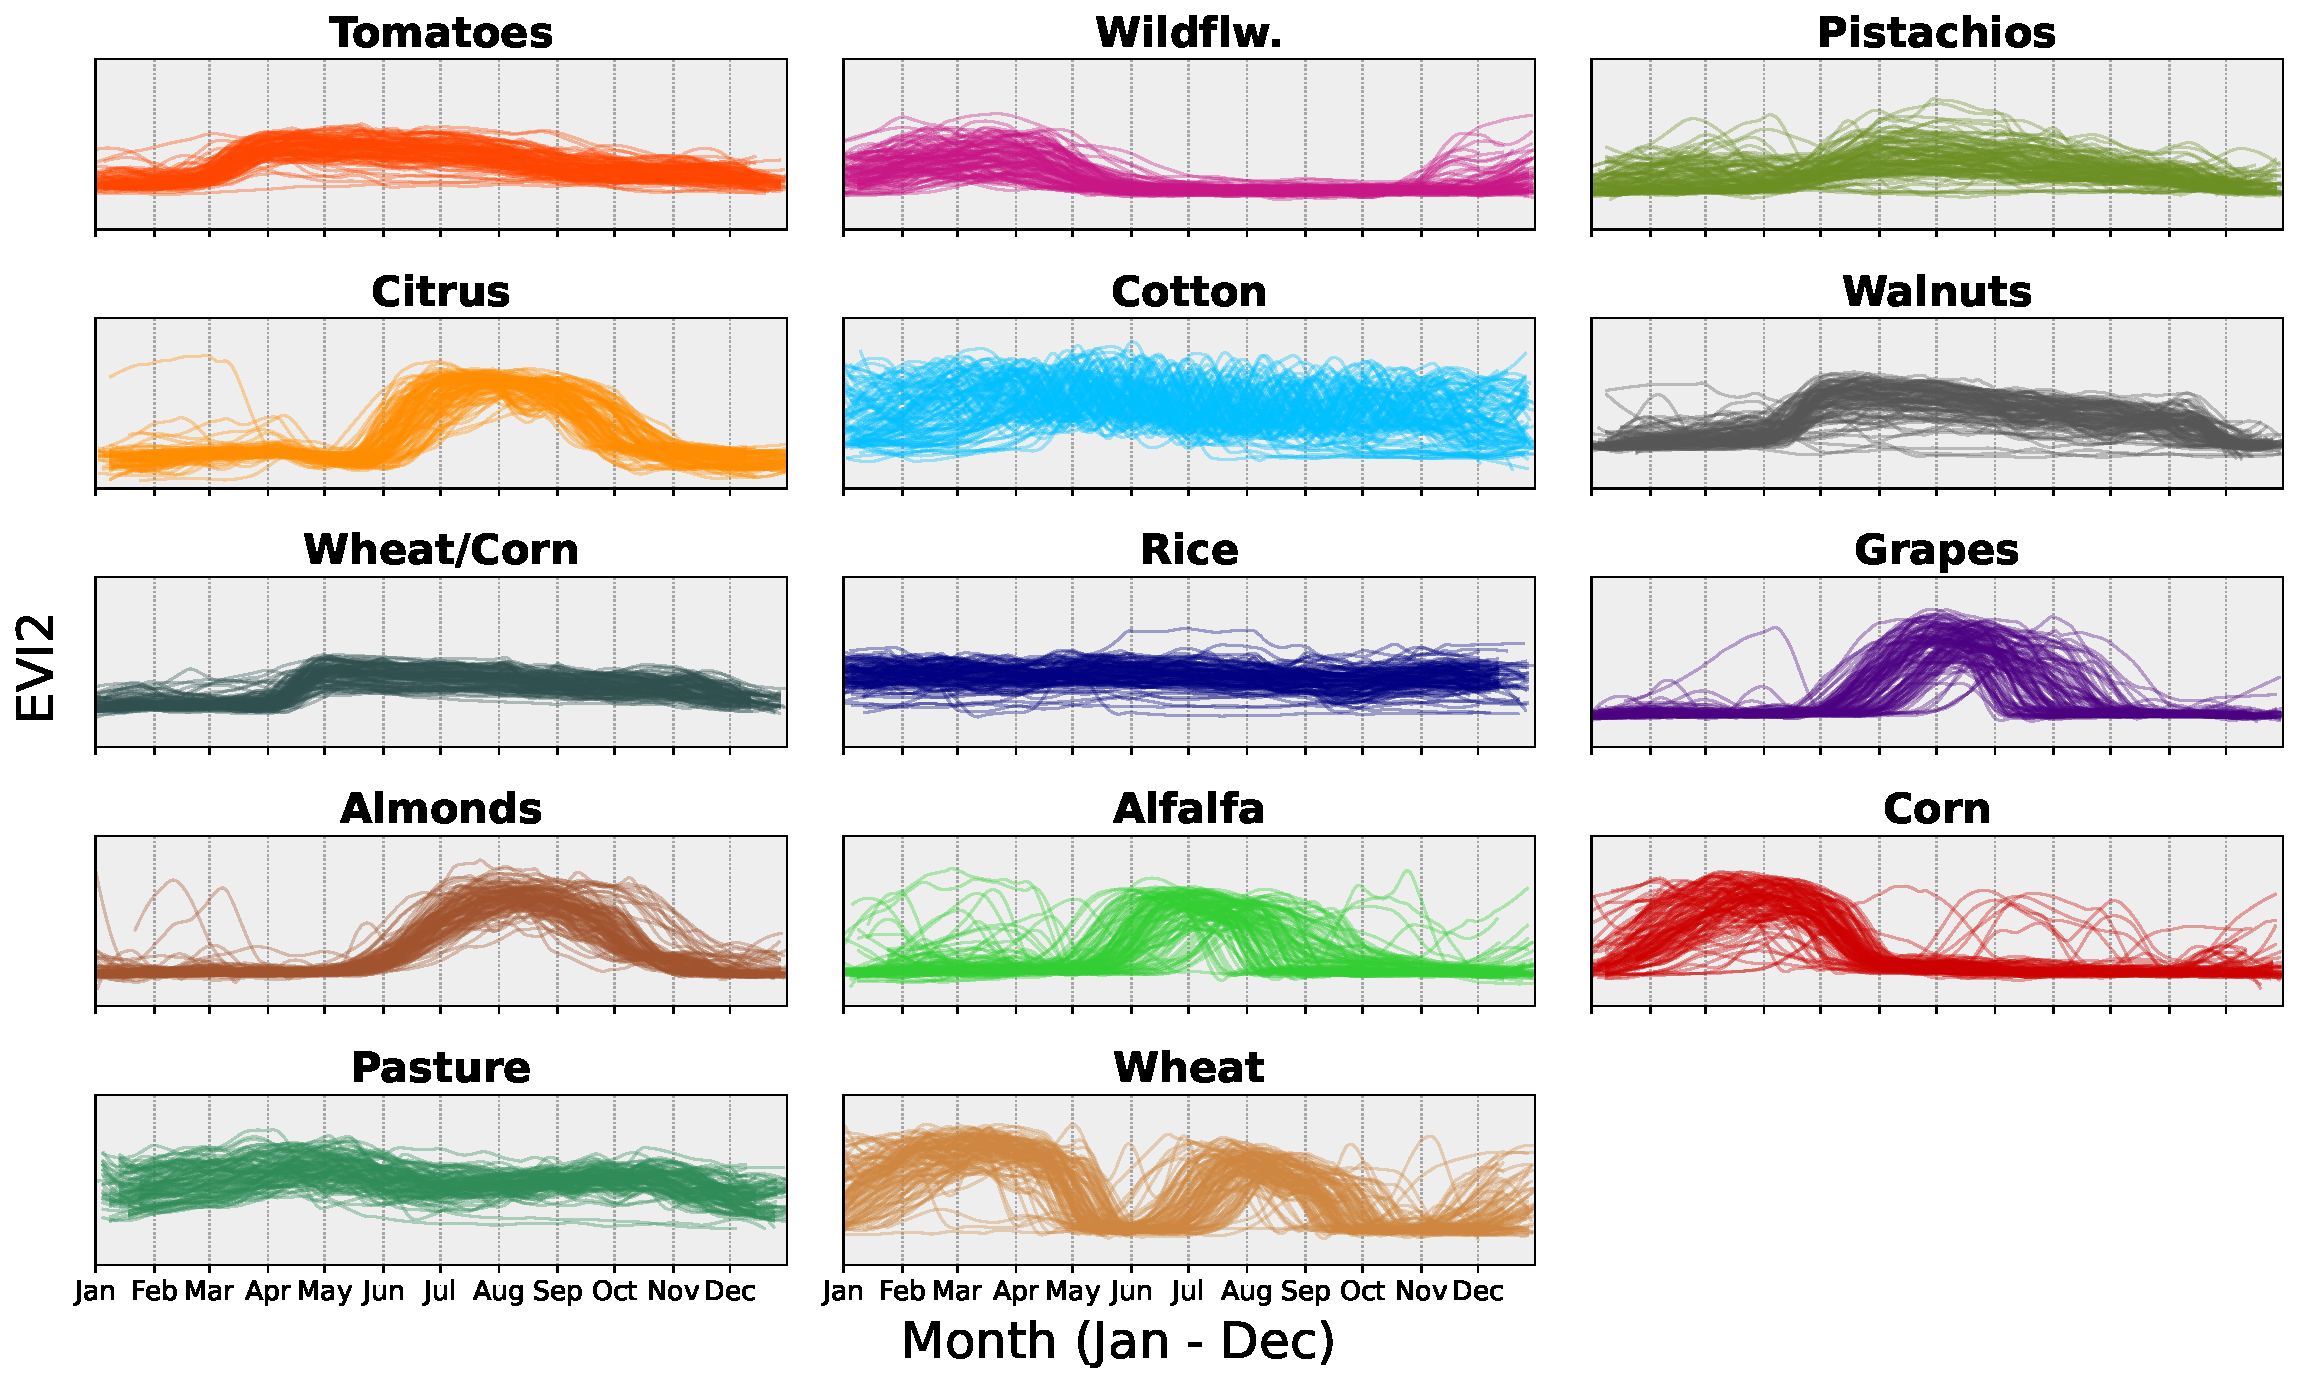
\includegraphics[width=0.7\linewidth]{figures/6_methodology/datasets/california_evi2.pdf}
\label{fig:evi2_california}
\fignote{Although only EVI2 is shown, which is an agricultural index calculated from Red and NIR and allows for easier visual differentiation of crop classes, the datasets consist of all 10 bands of Sentinel-2.}
\end{figure}

\begin{figure}[ht!]
\centering
\caption{EVI2 per crop class in Texas SITS dataset.}
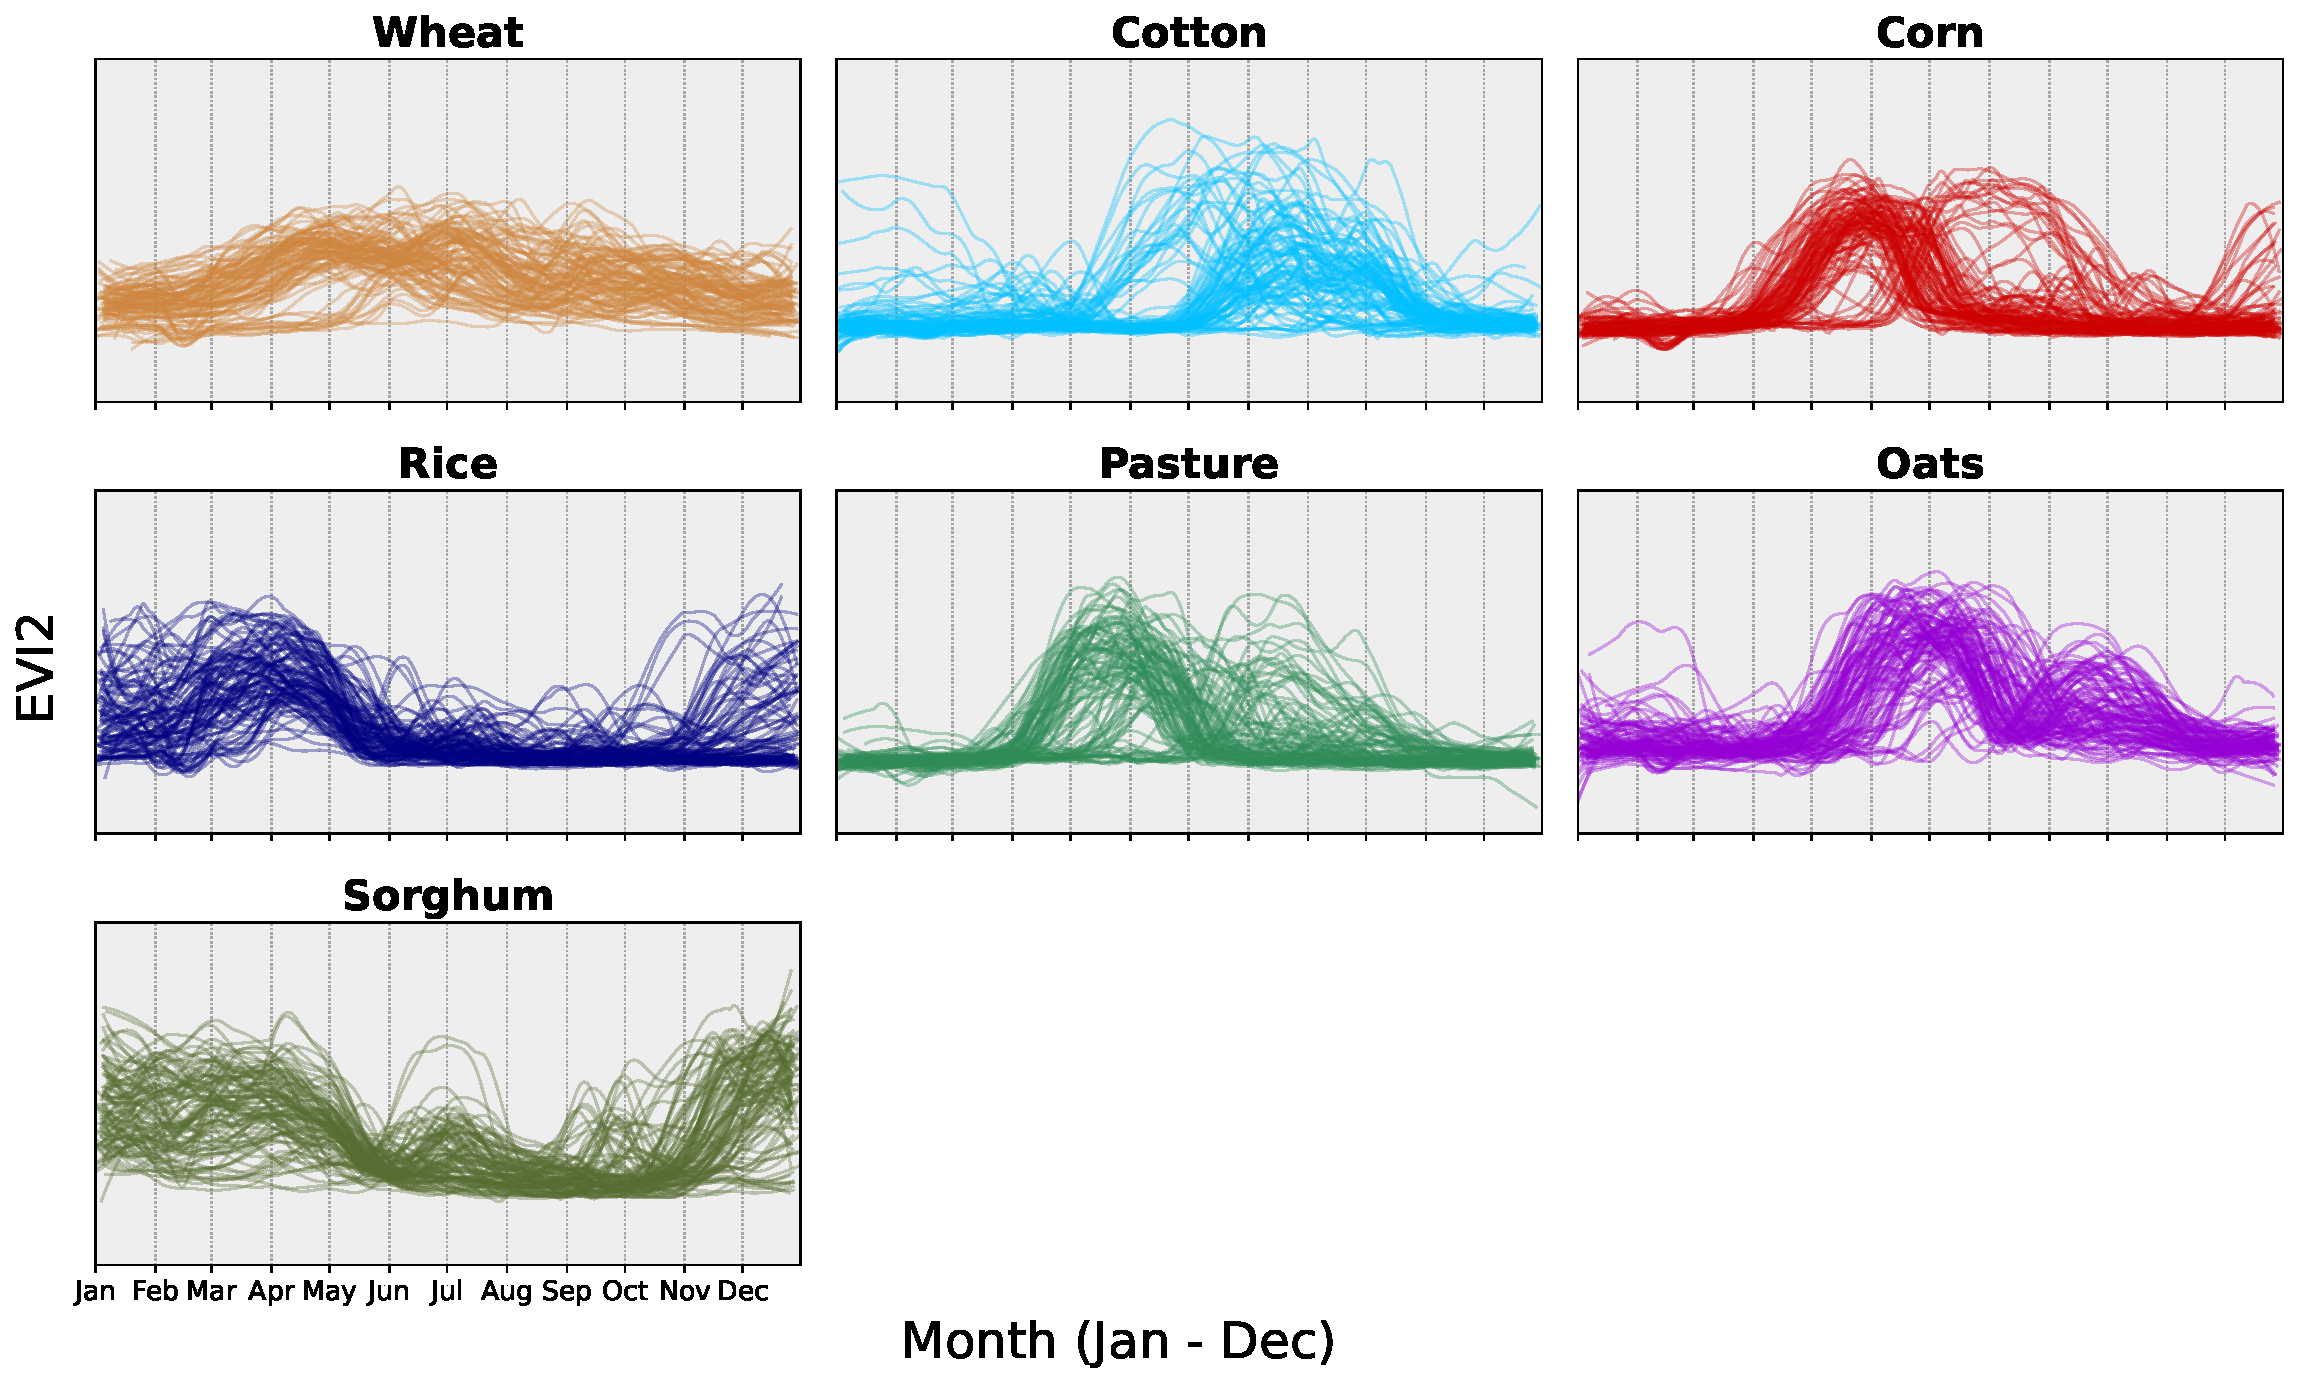
\includegraphics[width=0.7\linewidth]{figures/6_methodology/datasets/texas_evi2.pdf}
\label{fig:evi2_texas}
\fignote{Although only EVI2 is shown, which is an agricultural index calculated from Red and NIR and allows for easier visual differentiation of crop classes, the datasets consist of all 10 bands of Sentinel-2.}
\end{figure}

Finally, the evaluation strategy reflects the varying difficulty of the datasets. A more rigorous division between training, validation, and testing was implemented for Brazil compared to California and Texas. While the US datasets used a stratified split by samples (following \citep{pintodasilva2025lightweight}), the Brazilian dataset was split at the city level. This geographical split prevents spatial leakage and forces the model to generalize to unseen municipalities, making the metrics considerably more realistic and the task more challenging.

\section{The AgriGEE.lite library}
\label{sec:agl}

To facilitate the use of the methodology by other researchers, the lightweight \ac{SITS} download strategy has been coded in our open-source python library AgriGEE.lite. It is a parallel wrapper for \ac{GEE}, designed with the aim of abstracting the complexity of direct programming of the platform and solving performance bottlenecks in \ac{SITS} downloads. By default but optionally, the library abstracts preprocessing steps, such as applying sensor-specific cloud masks, atmospheric corrections, and band harmonization. The library can be installed using PyPI\footnote{PyPI: \url{https://pypi.org/project/agrigee-lite/}} and its source code can be downloaded/checked/reviewed in GitHub\footnote{GitHub: \url{https://github.com/mateuspinto/AgriGEE.lite}}.

The tool's architecture is specifically designed for use with GeoPandas, due to the widespread use of the latter library by remote sensing researchers. The workflow is organized into three main modules: \textbf{agl.sat}, responsible for defining sensors and other data sources; \textbf{agl.vis}, focused on exploratory data visualization; and \textbf{agl.get}, focused on data acquisition, whether parallel or not. One of the technical differences of the library is that downloads are performed by the aria2 utility, allowing the execution of multiple parallel connections outside the Python virtual machine, which enables parallel downloads without dealing with the problems inherent to parallelism and Python's GIL.

Although the methodology of this work specifically uses median statistics applied to Sentinel-2 images to generate the samples, AgriGEE.lite was developed to be agnostic with regard to the sensor and aggregation metric. As detailed in Table \ref{tab:agl_sats}, the library supports a wide range of data sources, including optical sensors (Sentinel-2, Landsat, MODIS), radar sensors (Sentinel-1, PALSAR), Cropland Rasters (MapBiomas, \ac{USDA}), and other products (ANADEM, SoilGrids).

\begin{landscape}
\begin{table}[ht]
\caption{Available data sources of AgriGEE.lite library.}
\centering
\small
\begin{tabular}{|l|p{4cm}|c|c|c|c|c|p{3cm}|}
\hline
\textbf{Name} & \textbf{Bands} & \textbf{Start} & \textbf{End} & \textbf{Region} & \textbf{Pixel size (meters)} & \textbf{Revisit Time} & \textbf{Variations} \\
\hline
Sentinel 2 & VIS, Re1-4, Nir, Swir1-2 & 2016-01-01 & Operational & Global & 10-60 & 5 days & BOA, TOA \\
\hline
Landsat 5 & VIS, Nir, Swir1-2 & 1984-03-01 & 2013-05-05 & Global & 30 & 16 days & - \\
\hline
Landsat 7 & VIS, Nir, Swir1-2, Pan & 1999-04-15 & 2022-04-06 & Global & 15-30 & 16 days & Pan-sharpened \\
\hline
Landsat 8 & VIS, Nir, Swir1-2, Pan & 2013-04-11 & Operational & Global & 15-30 & 16 days & Pan-sharpened \\
\hline
Landsat 9 & VIS, Nir, Swir1-2, Pan & 2021-11-01 & Operational & Global & 15-30 & 16 days & Pan-sharpened \\
\hline
HLS Landsat & Coastal, VIS, Nir, Swir & 2013-04-11 & Operational & Global & 30 & 2-3 days & - \\
\hline
HLS Sent-2 & Coastal, VIS, Re, Nir & 2015-11-30 & Operational & Global & 30 & 2-3 days & - \\
\hline
MODIS & Red, Nir & 2000-02-18 & Operational & Global & 250 & Daily & - \\
\hline
Sentinel 1 & VV, VH (C Band) & 2014-10-03 & Operational & Global & 10 & 5 days & GRD, ARD \\
\hline
JAXA PalSAR & HH, HV (L Band) & 2014-08-04 & Operational & Global & 25 & 15 days & GRD \\
\hline
Sat Embed & 64-dim embedding & 2017-01-01 & 2024-01-01 & Global & 10 & 1 year & - \\
\hline
Mapbiomas & 37 LULC Classes & 1985-01-01 & 2024-12-31 & Brazil & 30 & 1 year & - \\
\hline
ANADEM & Slope, Elevation, Aspect & Single & Single & S. Amer & 30 & Single & - \\
\hline
SoilGrids & WRB Soil Classes & Single & Single & Global & 250 & Single & - \\
\hline
\end{tabular}
\label{tab:agl_sats}
\end{table}
\fignote{The explanation for the abbreviations used in the table is as follows:

\begin{enumerate}
  \item \textbf{BOA -} Bottom of Atmosphere;
  \item \textbf{TOA -} Top of Atmosphere;
  \item \textbf{Pan-sharpened -} Can be downloaded with pan-sharp super resolution applied, increasing spatial resolution to 15 meters;
  \item \textbf{GRD -} Ground Range Detected;
  \item \textbf{ARD -} Analysis Ready Data.
\end{enumerate}
}
\end{landscape}


In addition to flexibility in sensor selection, the tool automates the calculation of spectral indices useful for agricultural and deforestation \ac{RS}, performed in the \ac{GEE} cloud prior to download. The library covers a wide spectrum of optical indices, including those for vegetation health and greenness (e.g., NDVI, EVI, SAVI, GNDVI, NDRE), water content detection (NDWI, MNDWI), and soil characteristics (BSI). Furthermore, specific indices for Synthetic Aperture Radar (SAR) data are implemented, such as the Radar Vegetation Index (RVI) and polarization ratios (VH/VV, HH/HV).

Similarly, for scenarios that require statistics other than the median, the library offers several spatial reducers allowing use in various experimental setups. The available statistics encompass measures of central tendency (mean, mode), dispersion (standard deviation, variance, minimum, maximum), and distribution shape (kurtosis, skewness). Users can also request arbitrary percentiles to capture specific segments of the data distribution.
\chapter{Methods for Learning from SITS Data}
\label{chapter:meth_model}

\begin{figure}[ht!]
    \centering
    \caption{Graphical abstract showing the whole training and inference stages.}
    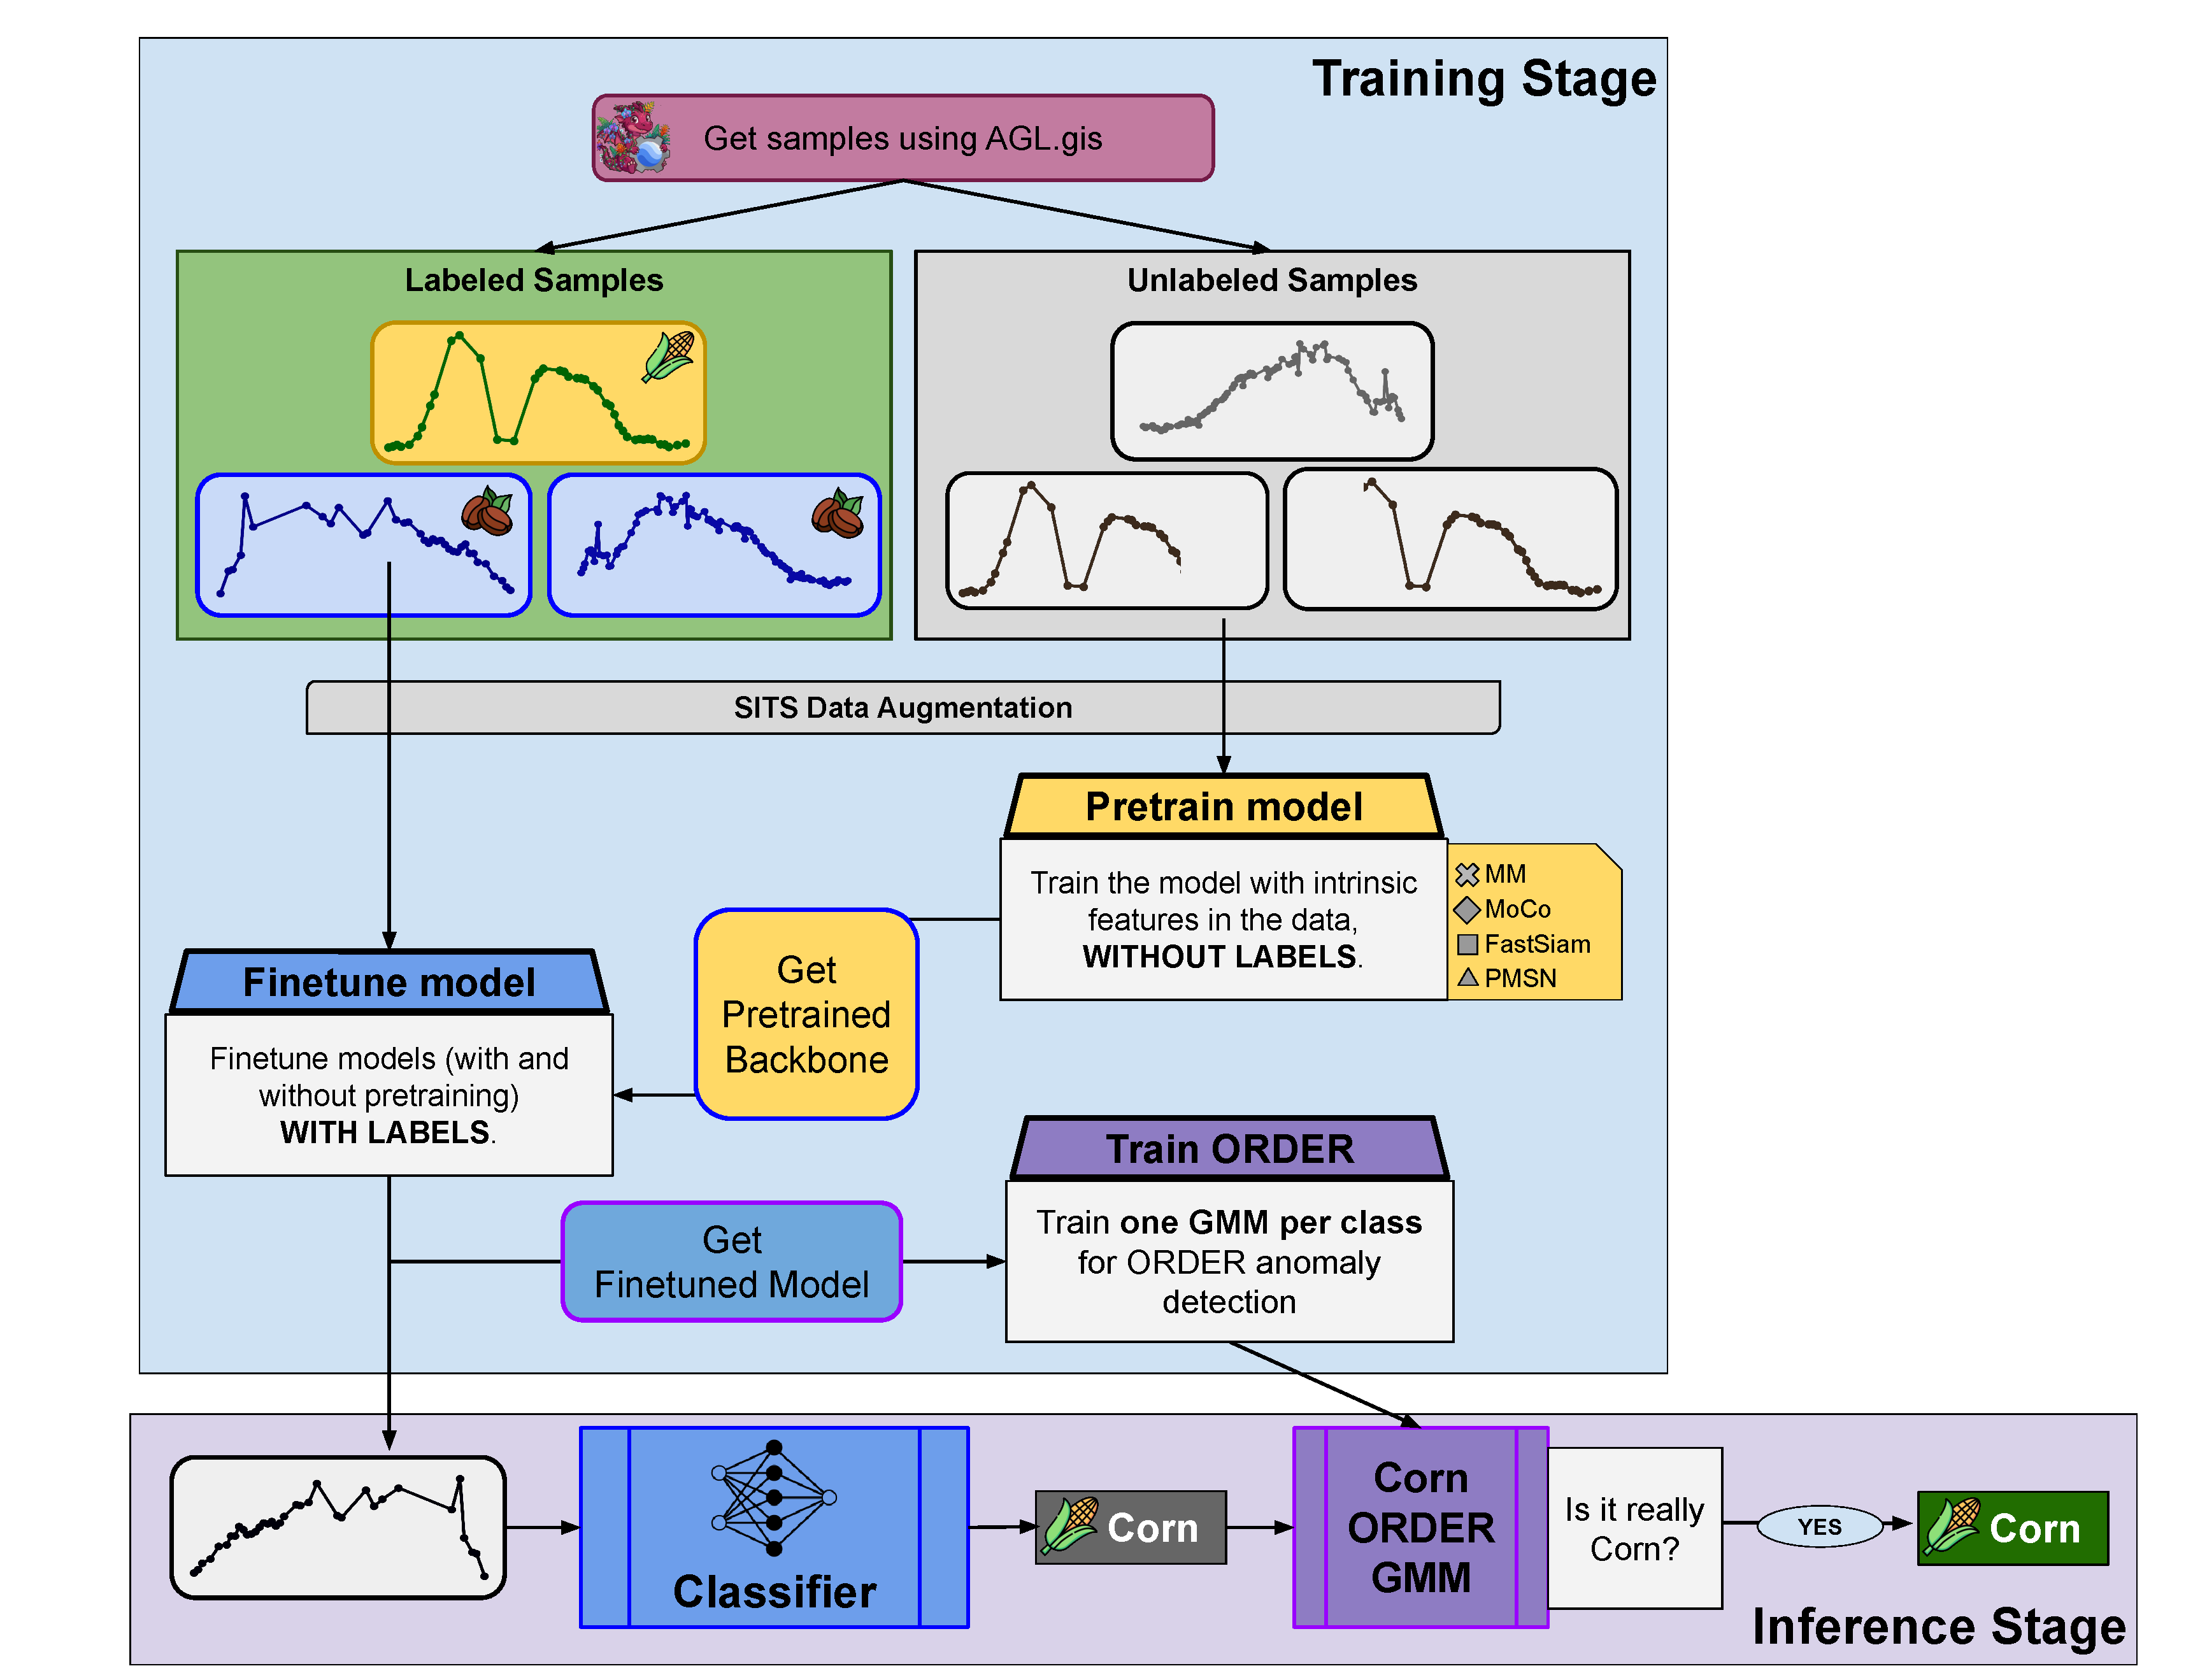
\includegraphics[width=1\linewidth]{figures/6_methodology/meth_graphical_abstract.pdf}
    \label{fig:meth_graphical_abstract}
\end{figure}

With the dataset already consolidated and the samples downloaded using what was presented in the previous chapter (see \autoref{chapter:meth_data}), this pipeline (see \autoref{fig:meth_graphical_abstract}) begins by differentiating between labeled and unlabeled samples (in this work, the unlabeled samples are the same as the labeled ones, but always using all the samples in the dataset). Both undergo a data augmentation process, and the unlabeled samples are used as pre-training for the model. With the trained model backbone, the labeled samples are used for fine-tuning, creating a model capable of classifying predictions. Finally, a \ac{GMM} per class is trained for the \ac{ORDER} method of anomaly detection. In the inference stage, a new sample is received and classified. It receives a class, and the GMM specific to that predicted class checks if there was an anomaly in the model or not. If not, the prediction is confirmed. This pipeline is explained in detail in this chapter.

To establish a robust baseline for \ac{DL} models, this work implemented \ac{SL}-based methodologies. Although \ac{DL} models operate directly on raw data, traditional algorithms require a preliminary feature engineering step to transform the temporal dimension into a structured tabular format, since \ac{SL} models do not handle data of varying sizes.

The preprocessing strategy adopted for \ac{SL} models consisted of reducing the temporal dimensionality by calculating monthly averages. As defined in the implemented transformation pipeline, the time series, originally composed of sequences of \ac{DoY}s and spectral bands, were resampled to 12 fixed time steps (one per month), where the values of each band were aggregated. The resulting vector for each sample was then normalized and flattened to serve as input to the classifiers.

Four SL models were evaluated: RF, SVM, GB through the LGBM library, and an MLP. However, it is known that the process of choosing/creating the best features is time-consuming and often impractical. Therefore, the literature is shifting towards DL models, due to their ability to also learn features.


\section{Deep Architectures for SITS Modeling}
\label{sec:models_supervised}

To evaluate the performance of different paradigms of DL models in SITS crop classification, this work implemented five distinct architectures. These range from attention-based models (Transformers) to recurrent, convolutional, and post-Transformer approaches. All networks share a common input structure, where time series of satellite images are processed to generate embeddings that feed a final linear classifier.

\noindent{\textbf{SITS-CNN:}} To evaluate the performance of convolutional networks, SITS-ConvNeXt was designed, based on the modern ConvNeXt CNN. This architecture adapts the blocks of the ConvNeXt network, originally designed for 2D computer vision, to handle SITS. The implementation treats the temporal dimension and spectral bands as an image, applying convolutions with large kernels (size 7) to capture broad temporal contexts. The model uses convolutional stem layers followed by ConvNeXt residual blocks, layer normalization, and global pooling to extract the final embeddings for classification.

\noindent{\textbf{SITS-LSTM:}} To represent the recurrent network class, the SITS-LSTM model was developed using BiGRU blocks. Unlike classical approaches, this model also incorporates Positional Encoding injection into the input embeddings before the recurrent layer, allowing the network to use explicit information about the \ac{DoY}, so that the comparison with other models is fairer. The output of the recurrent network undergoes layer normalization and dropout before classification, using the final hidden state aggregated via max pooling across the temporal dimension to generate the final embeddings for classification.

\noindent{\textbf{SITS-BERT:}} The SITS-BERT model was implemented strictly following the original architecture proposed in the literature. The model consists of a Transformer encoder only composed of 3 layers, with 8 attention heads and a hidden dimension of 256. The time series input undergoes a linear projection followed by the addition of Positional Encoding based on \ac{DoY}.

\noindent{\textbf{SITS-BERT++:}} As an evolution of this architecture, SITS-BERT++ was used. The number of attention heads was increased to 12 according to the author's work. However, due to implementation restrictions of the PyTorch library, which requires the hidden dimension to be divisible by the number of attention heads, the size of the hidden dimension was adjusted from 256 (original) to 252. SITS-BERT++ also incorporates another attention section for reconstruction and uses Swish activation in the Transformer layers and GeLU in the linear layers.

\noindent{\textbf{SITS-Mamba:}} Exploring the frontier of post-transformer models, SITS-Mamba was implemented, based on the Mamba architecture and Selective State Space Models (S6). The model consists of a stack of Mamba blocks (MambaBlocks), which replace the quadratic self-attention mechanism of Transformers with a linear selection mechanism $O(L)$. In the proposed implementation, the input data and DoY are projected and summed, passing sequentially through three layers of Mamba blocks with a hidden dimension of 256.

\section{Self-Supervised Learning for SITS}
\label{sec:models_selfsup}

\begin{figure}[ht!]
\centering
\caption{Graphical abstract showing the different SSL pretrainings with SITS data.}
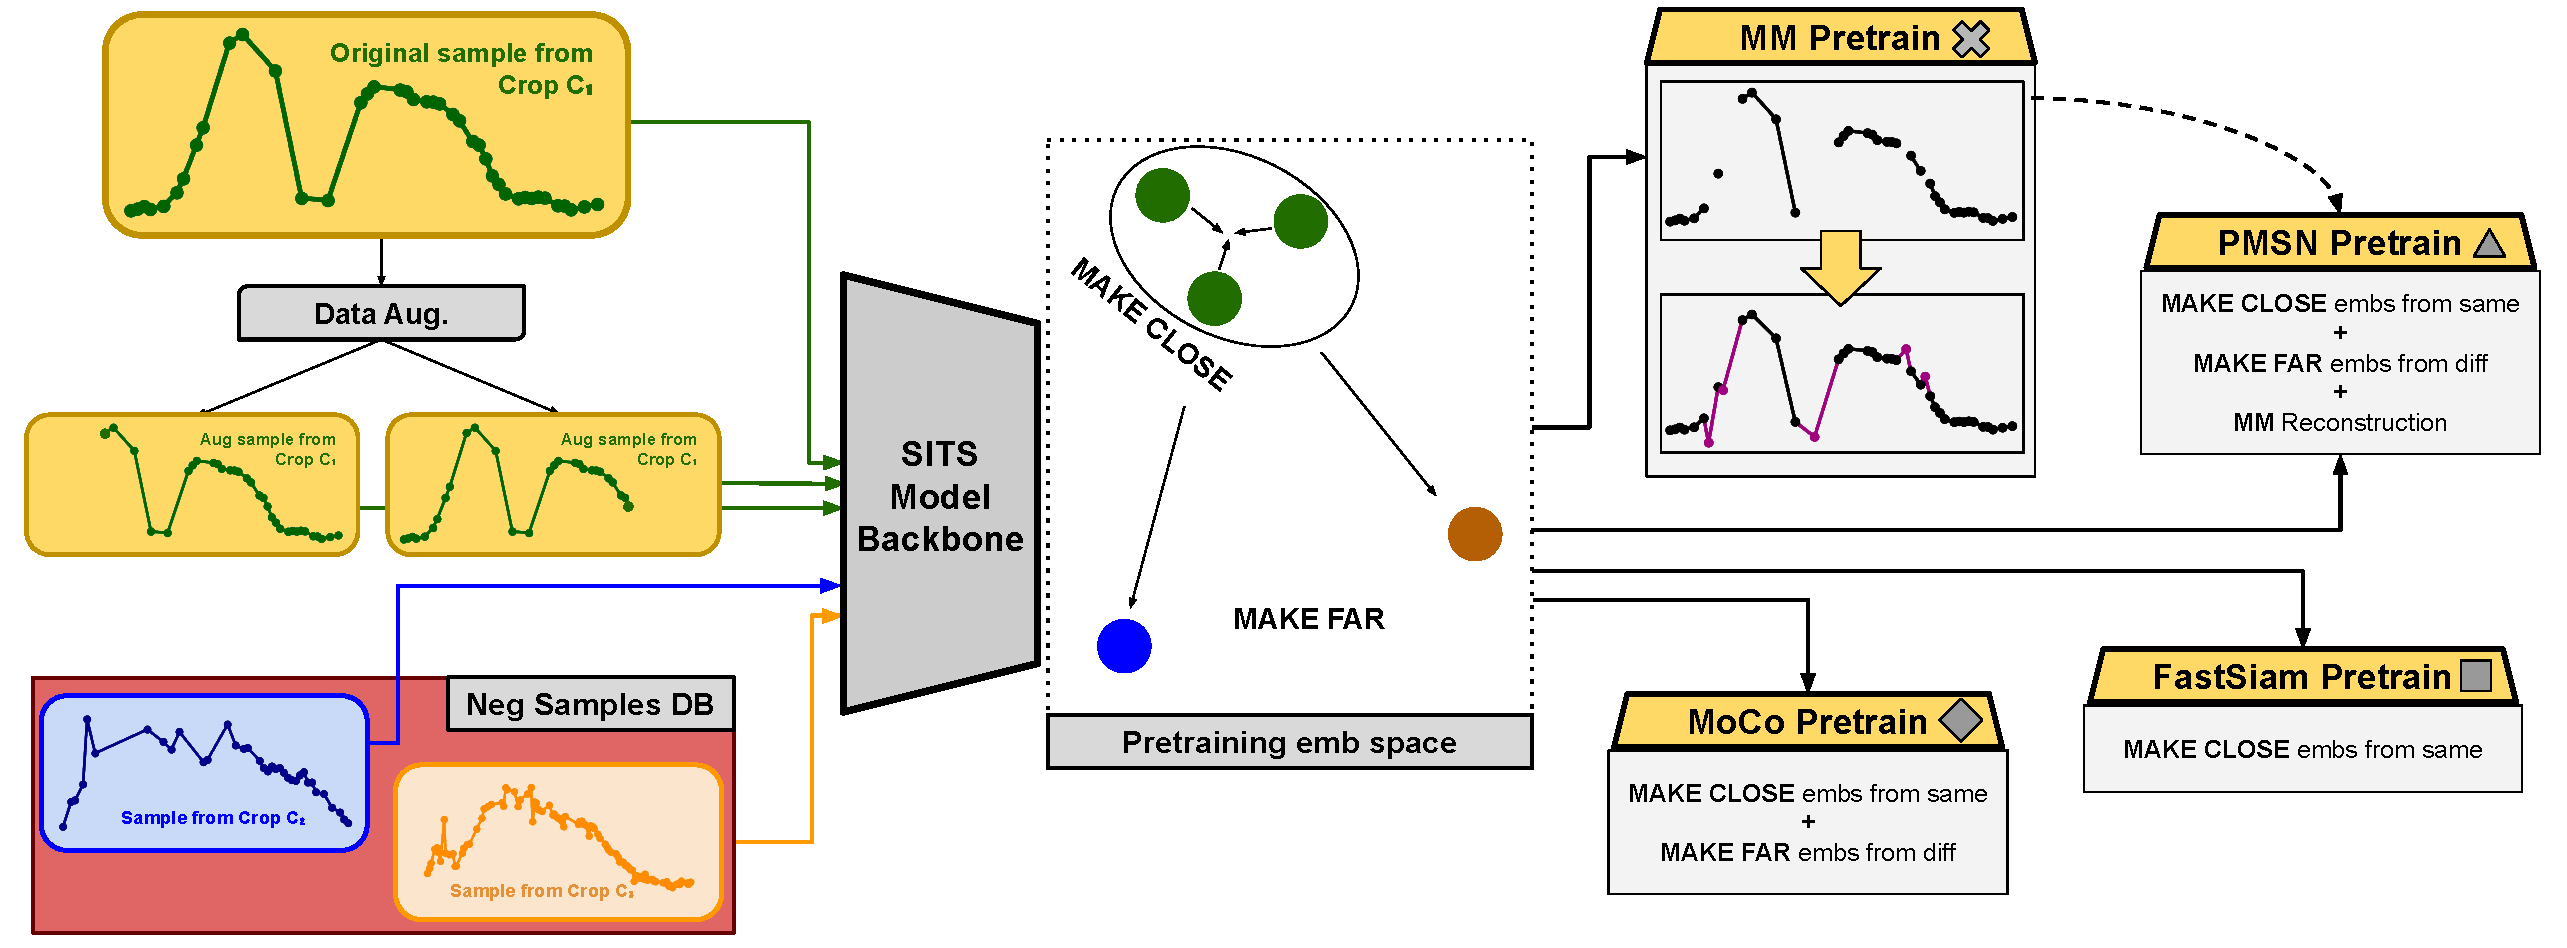
\includegraphics[width=1\linewidth]{figures/6_methodology/meth_ssl.pdf}
\label{fig:meth_ssl}
\end{figure}

To mitigate the scarcity of labeled data from unlabeled \ac{SITS}, this work explores and compares four \ac{SSL} strategies. The selected approaches cover the paradigms of masked modeling/reconstruction, contrastive learning, non-contrastive learning, and hybrid methods.

All strategies use a data augmentation pipeline designed specifically for \ac{SITS} data, in the first paradigm as traditional sample augmentation and the last three to compare augmentations with the data itself and train based on similarities. The transformations applied include: random temporal shift, which simulates variations in planting/harvesting dates; random removal of timestamps, simulating data loss due to clouds or sensor errors; and random swapping of the order of neighboring timestamps. In addition, data normalization is applied consistently.

The first approach evaluated is based on reconstruction via Masked Modeling (MIM). In this configuration, a binary mask is applied to the input, corrupting a percentage of the timestamps in the time series, replacing some timestamps with a token representing the absence of data. The model is trained to predict the values of the original bands of the hidden timestamps, minimizing the Mean Squared Error (MSE) calculated exclusively on the masked elements. This task forces the encoder to learn temporal dependencies and spectral correlations to infer the missing context.

The second strategy employs Momentum Contrast (MoCo), a contrastive method that uses a dynamic dictionary mechanism. The model operates with two encoders: a query encoder, updated via backpropagation, and a key encoder, whose weights are updated via exponential moving average (momentum update) of the query encoder weights. A memory bank is used to store past negative samples, allowing the use of a large number of negatives without the need for excessively large batches. The InfoNCE NT-Xent loss function is used to maximize the similarity between positive view representations while minimizing similarity with negative keys.

The third approach uses FastSiam, a non-contrastive method that does not require the use of negative pairs. The architecture consists of Siamese networks where one of the branches receives an additional prediction head (MLP). To prevent the representation from collapsing into a trivial solution, the stop-gradient operation is applied to the opposite branch. The goal is to maximize the negative cosine similarity between the prediction of one augmented view and the projection of the other view, learning invariance to the applied transformations.

Finally, we evaluate Prior Matching for Siamese Networks (PMSN), a hybrid approach that integrates data masking with prototype-based learning. In this method, an anchor view of the time series is artificially masked, while a target view remains intact, undergoing only standard augmentations. Both representations are projected into a space of trainable prototypes. The loss function seeks to align the probability distribution of the masked anchor with that of the target view on these prototypes, encouraging the model to recognize the semantics of the sample even in the absence of significant parts of the temporal information.

\section{Anomaly Detection and Open Set for SITS}
\label{sec:models_anomaly}

To refine the predictions of SITS classification models, we created an approach focused on the anomaly detection and \ac{OSR} literatures. We propose the \ac{ORDER} method. Although inspired by the GeMOS \ac{OSR} framework~\cite{vendramini2021opening}, \ac{ORDER} substantially advances the methodology by addressing a recurrent challenge in threshold-based methods: the automatic identification of optimal decision boundaries. While \ac{GeMOS} is characterized as a plug-and-play approach that couples GMMs to pretrained neural networks using their embeddings as features, it typically relies on fixed heuristics for rejection. \ac{ORDER} overcomes this limitation by introducing a supervised optimization cycle for hyperparameter optimization and automatic threshold definition. Consequently, the most significant contribution of \ac{ORDER} lies in this fundamental shift in application scope. Unlike the original GeMOS framework, which is primarily designed for \ac{OSR} tasks to identify entirely new and unseen classes, \ac{ORDER} is strictly not intended for open-set scenarios. Instead, its core purpose is the precise discrimination between correct and incorrect predictions within known classes, serving as a robust anomaly detection mechanism to facilitate rigorous dataset cleaning and quality control.

\begin{figure}[ht!]
    \centering
    \caption{Graphical abstract showing the ORDER anomaly detection.}
    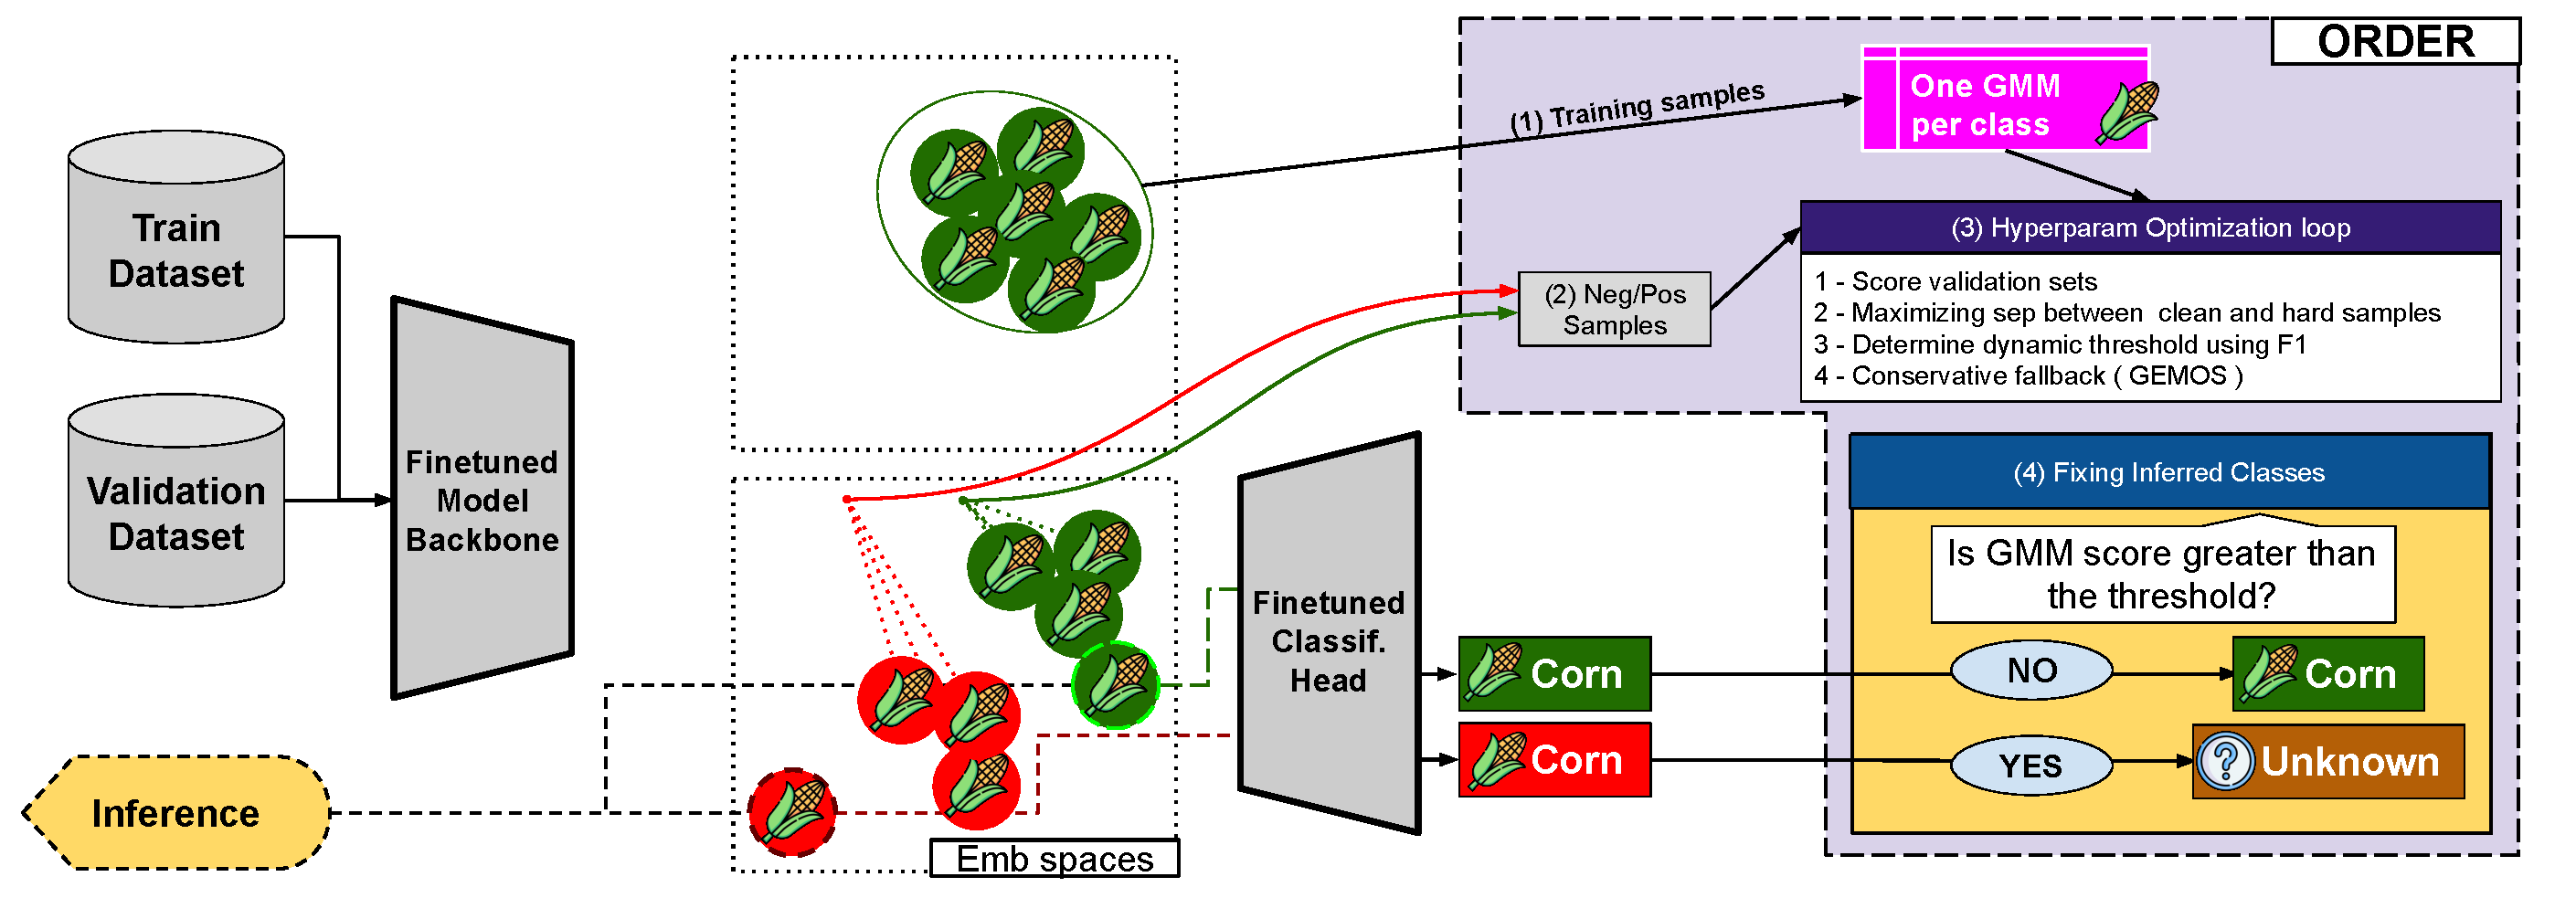
\includegraphics[width=1\linewidth]{figures/6_methodology/meth_models.pdf}
    \label{fig:meth_anomaly}
\end{figure}

As with \ac{GeMOS}, the \ac{ORDER} method uses a dedicated GMM per class, and its main flow iterates over the classes predicted by the base crop classification model. The process begins with feature extraction: in step 1, all correctly classified samples in the training set have their embeddings -  i.e., the intermediate latent representations of the \ac{DL} model - copied to form the training basis for the \ac{GMM} of that class. In step 2, the method processes the validation set, dividing the embeddings into two groups: positive samples (correct classifications) and negative samples (incorrect classifications), which simulate the behavior of hard negatives.

The core contribution of the method lies in step 3, where the stochastic optimization loop of the \ac{GMM} hyperparameters begins. Unlike the standard \ac{GeMOS} approach, which tends to fix the \ac{GMM} hyperparameters (by fixing the number of components), \ac{ORDER} implements an active search for the best configuration through a custom objective function. As detailed in sub-steps 3.1 and 3.2, for each hyperparameter attempt, the candidate model is trained and then used to calculate the log-likelihood of the positive and negative validation groups. The success criterion is not only the fit to the data, but the maximization of the AUC resulting from the separation between these scores. This forces the model to learn a distribution that not only represents the class, but maximizes the distinction between reliable patterns and classifier errors (anomalies).

Solving the threshold definition problem, step 3.3 dynamically establishes the decision boundary. Instead of applying an arbitrary percentile to the training data, the algorithm computes the precision and recall curves based on the validation scores and selects the threshold that maximizes the F1-Score. This strategy adapts the detector's sensitivity to the specific density and dispersion of each class. Finally, sub-step 3.4 acts as a fallback mechanism: if the size of the training set, positive samples, or negative samples is too small for optimization, the method automatically reverts to a conservative configuration, adjusting a \ac{GMM} with one component and setting the cutoff at the 2.5th percentile (basically the standard \ac{GeMOS}, but with values better adjusted for the specific case of \ac{ORDER}), ensuring robustness even in scenarios of very scarce data, or that the model gets the vast majority of samples in the validation sets right or wrong. Although the method has also been tested for OSR, the main focus is anomaly detection for Closed Set.
\chapter{Experimental Setup}
\label{chapter:exp_setup}

As an experimental setup, scenarios with different levels of scarcity of labeled data will be used to evaluate the performance of the trained models. The scenarios include 0.1\%, 1\%, 10\%, and 70\% of the labeled data available in each dataset, with the minor exception that the Brazilian dataset does not present the 0.1\% scenario due to its limited number of labeled samples combined with the separation between training/validation/testing by city, as it was not possible to select 0.1\% of the cities while maintaining at least one sample in each class.

\section{Hardware and Software Used}

The experiments were conducted on an Azure virtual machine provided by \ac{IBGE}. The hardware consists of an AMD EPYC 7V13 processor (Zen 3 architecture) with 48 cores and a base frequency of 2.89 GHz, 448 GiB of RAM, and 2x NVIDIA A100 PCIe 80 GB GPUs, totaling 160 GB of video memory (VRAM). As for the base software, Ubuntu 24.04.2 LTS (Noble Numbat) distribution was used with Linux kernel version 6.14.0-1014-azure and NVIDIA driver 550.163.01. It is important to mention that this machine is well above the minimum required to run the experiments, so it was possible to run several experiments in parallel, saving a lot of development time.

Some less common libraries were used: hyperparameter search was performed by Optuna, and Intel's high-performance Scikit Learn patch, Scikit Learn Intelex, was used. Regarding the versions of all software, all experiments were run within a container orchestrated by Docker 28.3.0, build 38b7060. The image used as a base was the official Pytorch image, version 2.4.0-cuda12.4-cudnn9-devel. The other important packages were their respective versions: AgriGEE.lite 2.0.14, LightGBM 4.6.0, Optuna 4.6.0, Scikit Learn==1.7.2, and Scikit Learn Intelex 2025.10.0.


\section{Shallow Learning hyperparameter search space}

A hyperparameter search was performed for all SL model experiments, including \ac{ORDER} \ac{GMM}. This search was performed using the Tree-structured Parzen Estimator (TPE) \citep{watanabe2025treestructuredparzenestimatorunderstanding}, a sequential Bayesian optimization approach that constructs a probabilistic model of the objective function based on the history of past evaluations. The TPE works by modeling separate densities for good and bad performance configurations, guiding the search to regions of parameter space with a higher probability of maximizing the evaluation metric. For each experiment, the search process was configured with a limit of 100 trials, which is the minimum recommended by the Optuna library used.

For the \ac{SVM} model, the search strategy focused on the balance between regularization and kernel. The penalty parameter  was sampled from a log-uniform distribution within the interval. The hyperplane topology was varied through categorical selection between linear, RBF, and polynomial kernels; for the latter two, the coefficient alternated between the ``auto'' and ``scale'' scales, while the degree of the polynomial was adjusted by integer values between 2 and 5. Class balancing was used to deal with the imbalance commonly found in crop classification datasets.

As for \ac{RF}, the hyperparameter space explored both the number of \ac{DT}s and the pruning of individual trees. The number of estimators was evaluated in the range from 80 to 350, and the maximum depth between trees between infinity, 5, and 10. The granularity of the trees was chosen based on the criteria of node division (between 2 and 10) and leaf composition (between 1 and 4), also considering different strategies for the selection of max features attributes and the activation or not of bootstrap sampling.

The configuration of \ac{ORDER}'s \ac{GMM} is: the number of mixtures/groups was sought linearly between 1 and 10, while the covariance matrix was tested under the geometries ``full'', ``tied'', ``diag'', and ``spherical''. To ensure numerical stability during estimation, a regularization term was applied to the covariance diagonal, whose values were extracted from a logarithmic scale between 0.000001 and 0.001.

Unlike previous models, the \ac{LGBM} classifier did not search for hyperparameters. Early Stopping from the library was used, where training is automatically interrupted if there is no improvement in the evaluation metric on the validation set after a certain number of iterations, defined as 50. Thus, the architecture was instantiated with fixed base parameters -- 500 DT, maximum depth of 5, and balanced weights (similar to SVM) -- with the number of iterations and overfitting prevention determined by dynamic validation monitoring, very similar to what happens in DL model training.

\section{Deep Learning hyperparameters and training strategies}

An attempt was made to standardize the training hyperparameters for all \ac{DL} model training, with some minor variations explained in this section. The weights of the DL models were optimized using the AdamW algorithm \citep{loshchilov2019decoupledweightdecayregularization}, a well-established variant of the Adam \citep{kingma2017adammethodstochasticoptimization} optimizer that decouples the implementation of weight decay from adaptive gradient optimization, providing more efficient and stable L2 regularization. The standard weight decay of 0.05 was used for all training sessions. Furthermore, PyTorch WeightedRandomSampler\footnote{Pytorh WeightedRandomSampler API Documentation: \url{https://docs.pytorch.org/docs/stable/data.html\#torch.utils.data.WeightedRandomSampler}} was used to handle class imbalance, using weights as the inverse of the class ratio. This way, each batch has its samples more or less balanced across all supervised trainings, including those from ConfidNet.

The learning rate control followed a dynamic schedule consisting of two distinct phases. In the first 10 training epochs, the learning rate is incremented linearly, starting from 0 until reaching the base rate of 0.0001. This step is very important to stabilize the initial gradients, especially in models based on Transformers and Mamba, which tend to predict only the majority class when they do not go through this initial step, called warmup. As for the other models, such warmup can at most be seen as a loss of processing cycles. After the warmup period, the learning rate decreases following a cosine curve until it reaches zero at the end of the maximum number of epochs, theoretically allowing for smooth convergence at the local minima of the loss function.

The duration of training varied depending on the task. For the self-supervised pre-training stages, the maximum limit was set at 400 epochs (passed through the training dataset). For fine-tuning and supervised training from scratch, the limit was set at 100 epochs for routines with 70\% and 10\% of the training data, and 200 for few-shot routines with scarcer data (1\% and 0.1\%).

To mitigate overfitting and optimize the use of computational time, two monitoring strategies based on the validation set were used: Early Stopping, in which training is automatically interrupted if the loss function in the validation set does not improve for a patience period set at 10 consecutive epochs (20 for pre-training). And Model Checkpointing, in which at the end of the training process (either by the end of the epochs or by the activation of Early Stopping), the model weights are reverted to the state corresponding to the epoch where the lowest loss function was obtained in the validation set.

The models were trained using mixed precision to reduce VRAM usage and speed up processing - mainly because we use GPUs that allow BF16 mixed precision, with a batch size of 2048 samples (or 8192 for all pre-trainings).

\section{Evaluation Metrics}

A set of metrics consolidated in the literature was used. It is important to note that, in multi-class scenarios such as the one presented, traditional binary metrics (such as Precision, Recall, and F1-Score) require aggregation strategies to provide a single indicator of overall performance. Common strategies are:

\begin{itemize}
    \item \textbf{Micro Average:} Calculates metrics globally by summing the total true positives, false negatives, and false positives of all classes. It is useful when evaluating overall performance in individual instances, as it is influenced by majority classes.
    \item \textbf{Macro Average:} Calculates the metric for each class individually and then extracts the unweighted arithmetic mean. This approach treats all classes equally, penalizing models that perform poorly in minority classes.
    \item \textbf{Weighted Average:} Calculates the metric for each class and extracts the average weighted by the support (number of actual instances) of each class. This strategy takes into account data imbalance and was the most used in the proposed problem, since crops with more samples are usually those with greater economic interest and, consequently, those with greater importance in the evaluation.
\end{itemize}


\textbf{Confusion Matrix - } The confusion matrix provides a tabular view of the model's performance, contrasting the predicted classes with the actual classes. The Table \ref{tab:confusion_matrix} illustrates the structure for a binary problem, although it can be extended to multiclass problems by simply adding a row and column for each new class.

\begin{table}[ht]
\centering
\caption{Structure of a binary confusion matrix.}
\begin{tabular}{|c|c|c|}
\hline
\cellcolor{white} & \textbf{Actually Positive (1)} & \textbf{Actually Negative (0)} \\
\hline
\textbf{Predicted Positive (1)} & True Positive (TP) & False Positive (FP) \\
\hline
\textbf{Predicted Negative (0)} & False Negative (FN) & True Negative (TN) \\
\hline
\end{tabular}
\label{tab:confusion_matrix}
\end{table}

\textbf{Accuracy - } Accuracy measures the overall proportion of correct predictions relative to the total number of samples.

\begin{equation}
\text{Accuracy} = \frac{TP + TN}{TP + TN + FP + FN}
\end{equation}

\textbf{Precision - } Precision assesses the quality of positive predictions, indicating how many of the items classified as positive are actually positive.

\begin{equation}
\text{Precision} = \frac{TP}{TP + FP}
\end{equation}

\textbf{Recall (Sensitivity) - } Recall (or Sensitivity) measures the model's ability to correctly identify all true positive instances.

\begin{equation}
\text{Recall} = \frac{TP}{TP + FN}
\end{equation}

\textbf{Specificity - } Specificity measures the model's ability to correctly identify actual negative instances, indicating how well the model avoids false positives.

\begin{equation}
\text{Specificity} = \frac{TN}{TN + FP}
\end{equation}

\textbf{F1-Score - } The F1-Score is the harmonic mean between Precision and Recall, penalizing extreme values (such as a model that predicts only one class), and is particularly useful in unbalanced datasets.

\begin{equation}
\text{F1-Score} = 2 \cdot \frac{\text{Precision} \cdot \text{Recall}}{\text{Precision} + \text{Recall}}
\end{equation}

\textbf{Geometric Mean Score (G-Mean) - } The Geometric Mean (G-Mean) assesses the balance between performance in the majority and minority classes, calculated as the square root of the product of Sensitivity and Specificity.

\begin{equation}
\text{G-Mean} = \sqrt{\text{Sensitivity} \times \text{Specificity}}
\end{equation}

\textbf{Matthews Correlation Coefficient (MCC) - } The Matthews Correlation Coefficient is a robust metric for imbalanced datasets, as it takes into account the four components of the confusion matrix, returning a value between -1 and +1.

\begin{equation}
\text{MCC} = \frac{TP \cdot TN - FP \cdot FN}{\sqrt{(TP + FP)(TP + FN)(TN + FP)(TN + FN)}}
\end{equation}

\textbf{Area Under the ROC Curve (AUC-ROC) - } AUC-ROC represents the probability that the model will classify a random positive example with a higher score than a random negative example. It is derived from the relationship between the True Positive Rate (TPR) and the False Positive Rate (FPR).

\begin{equation}
\text{TPR} = \frac{TP}{TP + FN}, \quad \text{FPR} = \frac{FP}{FP + TN}
\end{equation}

\begin{equation}
\text{AUC-ROC} = \int_{0}^{1} \text{TPR}(\text{FPR}) \, d(\text{FPR})
\end{equation}

\textbf{AUPR-Error - } The area under the Precision-Recall curve (AUPR) with a focus on error is often used in anomaly detection or OOD (Out-of-Distribution). Here, the unknown class is treated as the target class for calculating precision and recall.

\begin{equation}
\text{AUPR}_{\text{Error}} = \int_{0}^{1} \text{Precision}_{Neg}(\text{Recall}_{Neg}) \, d(\text{Recall}_{Neg})
\end{equation}

\textbf{AUPR-Success - } AUPR-Success refers to the standard metric of area under the Precision-Recall curve, where the known class is the target of interest.

\begin{equation}
\text{AUPR}_{\text{Success}} = \int_{0}^{1} \text{Precision}_{Pos}(\text{Recall}_{Pos}) \, d(\text{Recall}_{Pos})
\end{equation}

\textbf{FPR at N\% TPR - } This metric evaluates the robustness of the model at a specific security operating point. It measures the False Positive Rate (FPR) required to achieve at least $N\%$ True Positive Rate (TPR) (commonly $N=95\%$).

\begin{equation}
\text{FPR}@N\%\text{TPR} = \text{FPR}(\tau) \quad \text{,} \quad \text{TPR}(\tau) = \frac{N}{100}
\end{equation}

\textbf{Mean Squared Error (MSE) - } The Mean Squared Error is a metric used in regression, and measures the average of the squares of the differences between the predicted values (probabilities or regression values) and the actual values. In this work, it is used to evaluate the performance of the reconstruction pre-training.

\begin{equation}
\text{MSE} = \frac{1}{n} \sum_{i=1}^{n} (y_i - \hat{y}_i)^2
\end{equation}
\chapter{Results}
\label{chapter:results}

Quantitative evaluations were performed on the results, and qualitative evaluations were performed on some graphs, including visualizations of embeddings, for all experiments defined in the Experimental Setup (see Chapter \ref{chapter:exp_setup}), including \ac{SL} and \ac{DL} models, with and without pre-training, in different label scarcity modalities and showing ORDER anomaly detection. Approximately 100 experiments were performed for each dataset. Therefore, only the experiment with the best metric, according to F1 Weighted without anomalies, for each dataset was shown in more detail. The experiments were conducted on the three datasets created: Brazil, California, and Texas. 

\section{Shallow and Deep Baselines for SITS}

Initially, a baseline was established by training all \ac{SL} and \ac{DL} models in a fully supervised manner, using 70\% of the data for training. Tables \ref{tab:res_scratch_brazil}, \ref{tab:res_scratch_california}, and \ref{tab:res_scratch_texas} present the Weighted F1, Accuracy, Specificity, G-Mean, ConfidNet metrics in the \ac{DL} and \ac{MLP} models (including False Positive Rates, AUC and AUPR), for the Brazil, California, and Texas datasets, respectively. This discrepancy highlights the superior capability of deep architectures, particularly Transformers and State Space Models (Mamba), in capturing complex temporal dependencies in spectrally similar classes, which are abundant in the tropical agriculture of Brazil. Also, compairing Max Class Probability AUC with ConfidNet AUC, it is well known that the results vary; sometimes the model itself is better, sometimes ConfidNet is better. This shows that ConfidNet presented poor results, since the strategy is specifically designed to generate a better Precision-Recall curve than the original model.

\begin{table}[ht!]
\centering
\caption{Training results from scratch using 70\% on training data in the Brazil dataset.}
\label{tab:res_scratch_brazil}
\resizebox{\textwidth}{!}{%
\begin{tabular}{lccccccccccccc}
\hline
\textbf{Model} & \textbf{} & \textbf{} & \textbf{} & \textbf{} & \textbf{G} & \textbf{Mcp} & \textbf{} & \textbf{Conf} & \textbf{AUPR} & \textbf{AUPR} & \textbf{Conf} & \textbf{Anom} & \textbf{w. A} \\
 & \textbf{F1} & \textbf{Acc} & \textbf{Spec} & \textbf{Mcc} & \textbf{Mea} & \textbf{Auc} & \textbf{Fpr95} & \textbf{Auc} & \textbf{S} & \textbf{E} & \textbf{AUPR} & \textbf{Rate} & \textbf{F1} \\ \hline
SVM & 77.7 & 78.3 & 97.4 & 74.3 & 89.9 & - & - & - & - & - & - & \textbf{2.6} & 78.5 \\
RF & 75.0 & 76.0 & 97.0 & 71.6 & 86.3 & - & - & - & - & - & - & \textbf{1.3} & 75.0 \\
LGBM & 78.0 & 78.8 & 97.4 & 74.7 & 89.5 & - & - & - & - & - & - & 4.3 & 77.9 \\
MLP & 79.2 & 80.0 & 97.6 & 76.4 & 90.6 & 80.5 & 64.0 & 76.3 & 92.6 & 41.1 & \textbf{65.0} & 6.6 & 80.2 \\ \hline
CNN & 83.8 & 84.0 & 98.1 & 80.9 & 91.7 & 81.8 & 63.6 & 82.8 & 95.7 & 46.1 & \textbf{61.5} & 4.2 & 85.3 \\
LSTM & 84.6 & 84.5 & 98.1 & 81.4 & 91.9 & 82.5 & \textbf{60.1} & \textbf{84.6} & \textbf{96.3} & \textbf{49.2} & 56.0 & 5.7 & 85.8 \\
BERT & 84.1 & 84.0 & 98.1 & 80.9 & \textbf{92.3} & 80.9 & 65.3 & 83.1 & 95.8 & 47.0 & 60.3 & 5.6 & 85.8 \\
BERT++ & \textbf{85.6} & \textbf{85.5} & \textbf{98.3} & \textbf{82.7} & \textbf{92.7} & \textbf{82.9} & 60.8 & \textbf{84.0} & \textbf{96.2} & \textbf{48.1} & 60.1 & 6.3 & \textbf{87.3} \\
MAMBA & \textbf{85.0} & \textbf{85.1} & \textbf{98.2} & \textbf{82.2} & 92.2 & \textbf{83.2} & \textbf{59.7} & 82.9 & \textbf{96.2} & 44.2 & 55.8 & 3.4 & \textbf{85.9} \\ \hline
\end{tabular}%
}
\end{table}

\begin{table}[ht!]
\centering
\caption{Training results from scratch using 70\% on training data in the Texas dataset.}
\label{tab:res_scratch_texas}
\resizebox{\textwidth}{!}{%
\begin{tabular}{lccccccccccccc}
\hline
\textbf{Model} & \textbf{} & \textbf{} & \textbf{} & \textbf{} & \textbf{G} & \textbf{Mcp} & \textbf{} & \textbf{Conf} & \textbf{AUPR} & \textbf{AUPR} & \textbf{Conf} & \textbf{Anom} & \textbf{w. A} \\
 & \textbf{F1} & \textbf{Acc} & \textbf{Spec} & \textbf{Mcc} & \textbf{Mea} & \textbf{Auc} & \textbf{Fpr95} & \textbf{Auc} & \textbf{S} & \textbf{E} & \textbf{AUPR} & \textbf{Rate} & \textbf{F1} \\ \hline
SVM & 98.8 & 98.8 & \textbf{99.8} & 98.4 & 98.9 & - & - & - & - & - & - & \textbf{0.1} & 98.9 \\
RF & 97.9 & 98.0 & 99.6 & 97.3 & 96.2 & - & - & - & - & - & - & \textbf{0.1} & 97.9 \\
LGBM & 98.9 & 98.9 & \textbf{99.8} & 98.5 & 98.2 & - & - & - & - & - & - & \textbf{0.1} & 98.9 \\
MLP & 99.1 & 99.1 & \textbf{99.8} & 98.8 & 99.2 & 96.2 & 20.4 & \textbf{76.2} & \textbf{99.6} & \textbf{3.1} & 80.9 & \textbf{0.2} & 99.2 \\ \hline
CNN & \textbf{99.5} & \textbf{99.5} & \textbf{99.9} & \textbf{99.4} & 99.4 & \textbf{97.7} & \textbf{7.8} & 51.7 & 99.5 & 0.5 & 98.3 & \textbf{0.1} & \textbf{99.6} \\
LSTM & \textbf{99.6} & \textbf{99.6} & \textbf{99.9} & \textbf{99.5} & \textbf{99.5} & \textbf{97.7} & \textbf{7.8} & 35.5 & 99.4 & 0.3 & \textbf{99.0} & \textbf{0.1} & \textbf{99.7} \\
BERT & \textbf{99.5} & \textbf{99.5} & \textbf{99.9} & 99.3 & 99.4 & 96.9 & 15.0 & 33.2 & 99.1 & 0.4 & \textbf{99.3} & \textbf{0.1} & 99.5 \\
BERT++ & \textbf{99.5} & \textbf{99.5} & \textbf{99.9} & \textbf{99.4} & \textbf{99.5} & 96.9 & 13.6 & \textbf{89.4} & \textbf{99.9} & \textbf{21.2} & 52.7 & \textbf{0.2} & \textbf{99.6} \\
MAMBA & \textbf{99.6} & \textbf{99.6} & \textbf{99.9} & \textbf{99.5} & \textbf{99.6} & \textbf{98.4} & \textbf{6.3} & 45.4 & \textbf{99.6} & 0.3 & 97.4 & \textbf{0.1} & \textbf{99.7} \\ \hline
\end{tabular}%
}
\end{table}

\begin{table}[ht!]
\centering
\caption{Training results from scratch using 70\% on training data in the California dataset.}
\label{tab:res_scratch_california}
\resizebox{\textwidth}{!}{%
\begin{tabular}{lccccccccccccc}
\hline
\textbf{Model} & \textbf{} & \textbf{} & \textbf{} & \textbf{} & \textbf{G} & \textbf{Mcp} & \textbf{} & \textbf{Conf} & \textbf{AUPR} & \textbf{AUPR} & \textbf{Conf} & \textbf{Anom} & \textbf{w. A} \\
 & \textbf{F1} & \textbf{Acc} & \textbf{Spec} & \textbf{Mcc} & \textbf{Mea} & \textbf{Auc} & \textbf{Fpr95} & \textbf{Auc} & \textbf{S} & \textbf{E} & \textbf{AUPR} & \textbf{Rate} & \textbf{F1} \\ \hline
SVM & 97.2 & 97.2 & \textbf{99.8} & 96.7 & 98.2 & - & - & - & - & - & - & 0.9 & 7.4 \\
RF & 95.3 & 95.3 & 99.6 & 94.5 & 96.4 & - & - & - & - & - & - & \textbf{0.3} & 95.3 \\
LGBM & 96.2 & 96.2 & 99.7 & 95.6 & 97.7 & - & - & - & - & - & - & 1.2 & 96.7 \\
MLP & 97.0 & 97.0 & \textbf{99.8} & 96.5 & \textbf{98.6} & 92.9 & 41.8 & 59.3 & 98.2 & 3.4 & \textbf{76.8} & 1.0 & 97.5 \\ \hline
CNN & \textbf{98.2} & \textbf{98.2} & \textbf{99.8} & \textbf{97.9} & \textbf{98.6} & 95.3 & 22.5 & \textbf{94.8} & \textbf{99.9} & 36.4 & 25.9 & 0.7 & \textbf{98.2} \\
LSTM & 97.4 & 97.4 & \textbf{99.8} & 97.0 & 97.2 & \textbf{95.4} & \textbf{19.0} & \textbf{95.6} & \textbf{99.9} & \textbf{49.1} & 19.9 & 1.0 & 97.9 \\
BERT & \textbf{98.0} & \textbf{98.0} & \textbf{99.8} & \textbf{97.6} & 98.5 & \textbf{95.7} & \textbf{16.6} & 32.6 & 96.9 & 1.4 & \textbf{97.8} & \textbf{0.5} & \textbf{98.2} \\
BERT++ & 97.7 & 97.7 & \textbf{99.8} & 97.4 & \textbf{98.6} & 95.1 & 21.3 & 94.1 & \textbf{99.8} & \textbf{42.7} & 27.9 & 1.4 & \textbf{98.1} \\
MAMBA & 97.9 & 97.9 & \textbf{99.8} & \textbf{97.6} & \textbf{98.8} & \textbf{95.4} & 19.7 & 90.9 & 99.7 & 31.3 & 50.1 & 0.8 & 98.0 \\ \hline
\end{tabular}%
}
\end{table}

As expected, it was noted that the Brazilian dataset presents the worst metrics in all models when compared to those from Texas and California. In the Brazil dataset (see \autoref{tab:res_scratch_brazil}), the best \ac{DL} models (SITS-BERT++ and SITS-Mamba) achieved a Weighted F1 score of around 85\%, while the \ac{SL} models (such as SVM and LGBM) scored below 80\%. This increase also occurred, but to a lesser extent, in the California dataset (see \autoref{tab:res_scratch_california}), where \ac{DL} models such as SITS-BERT and SITS-LSTM were close to 98\% F1 Weighted, while \ac{SL} models were close to 95\%, with the exception of \ac{SVM}, which remained partially competitive with around 97\%. The reduced gap between SL and DL in California suggests that the spectral separability of crops in this region is naturally higher, allowing even simpler models like \ac{SVM} to find good decision boundaries. The Texas dataset (see \autoref{tab:res_scratch_texas}) was the easiest, with architectures such as SITS-LSTM and SITS-ConvNeXt achieving metrics above 99\%, with \ac{SVM} also remaining competitive with a Weighted F1 score close to 99\%. 

As for the results referring to the ConfidNet anomaly detection baseline, the opposite occurred: the metrics were worse for the California and Texas datasets, following what was observed by \cite{cheng2019leveraging} that the methodology tends not to work if the model makes classifications with very high result metrics. This happens because, in highly evaluation metric models, the confidence scores for both correct and incorrect predictions tend to cluster near 1 (overconfidence), making it difficult for the threshold-based approach of ConfidNet to distinguish between in-distribution errors and anomalies (as pointed out by the authors of the mod). Our ORDER method, on the other hand, showed solid results, improving the Weighted F1 metrics in all \ac{DL} models and in almost all \ac{SL} models, with the only exceptions being \ac{RF} and \ac{LGBM} in the California dataset (see \autoref{tab:res_scratch_california}).

\section{Pre-training analysis}

Before finetuning the pre-trained models on target data, the quality of the embeddings generated by the SSL strategies (Masked Modeling - MM, MoCo, FastSiam, and PMSN) using a linear KNN classifier on the validation data, trained with 1\% of the labels from the Brazil dataset and 0.1\% for California and Texas, with results summarized in Tables \ref{tab:pretraining_results_brazil}, \ref{tab:pretraining_results_california}, and \ref{tab:pretraining_results_texas}. The three best results from each table are in bold.

\begin{table}[ht!]
    \centering
    \caption{Pre-training results for Brazil dataset.}
    \begin{tabular}{llcccc}
        \toprule
        Model & Pretrain & Val Loss & $\sqrt{L_2}$ Emb & KNN Acc & KNN F1 \\
        \midrule
        CNN & MM & 2.61 & - & 51.63 & 54.56 \\
        CNN & MoCo & 6.47 & 0.09 & 49.12 & 53.49 \\
        CNN & FastSiam & -0.99 & 0.03 & 55.78 & 57.92 \\
        CNN & PMSN & 4.57 & 0.06 & 42.21 & 47.00 \\
        LSTM & MM & 3.0 & - & 53.89 & 58.02 \\
        LSTM & MoCo & 6.42 & 0.09 & 56.41 & 60.29 \\
        LSTM & FastSiam & -0.95 & 0.03 & 53.64 & 56.71 \\
        LSTM & PMSN & 4.88 & 0.06 & 57.54 & 61.23 \\
        BERT & MM & 2.64 & - & 57.16 & \textbf{62.18} \\
        BERT & MoCo & 6.43 & 0.09 & 60.43 & \textbf{63.80} \\
        BERT & FastSiam & -0.92 & 0.01 & 33.42 & 35.58 \\
        BERT & PMSN & 4.91 & 0.06 & 50.25 & 54.21 \\
        BERT++ & MM & 2.22 & - & 57.04 & 60.60 \\
        BERT++ & MoCo & 6.43 & 0.09 & 58.54 & 62.12 \\
        BERT++ & FastSiam & -0.7 & 0.02 & 38.57 & 43.26 \\
        BERT++ & PMSN & 4.78 & 0.06 & 48.37 & 52.31 \\
        Mamba & MM & 3.12 & - & 54.65 & 58.86 \\
        Mamba & MoCo & 6.45 & 0.09 & 58.92 & \textbf{62.34} \\
        \rowcolor{red!20} Mamba & FastSiam & -0.97 & 0.03 & 55.78 & 58.36 \\
        Mamba & PMSN & 4.18 & 0.06 & 56.16 & 59.31 \\
        \bottomrule
    \end{tabular}
    \label{tab:pretraining_results_brazil}
    \fignote{One should notice that a value close to $1/\sqrt{embsize}$ indicates that the representations are stable, and in all cases $1/\sqrt{embsize}\approx0.06$ in $\sqrt{L_2}$ Emb. If the value is greater or near this, the pretrained embeddings haven't all collapsed, meaning they aren't all nearly or identical. If it's lower, this situation is occurring, and the pretraining has failed.}
\end{table}

For the Brazil dataset (see Table \ref{tab:pretraining_results_brazil}), the MoCo strategy demonstrated consistent superiority in generating separable linear embeddings, achieving KNN accuracy greater than 62\% with backbones based on Transformer (BERT and BERT++) and post-Transformer (Mamba) models, second only to PMSN in SITS-CNN and SITS-LSTM. It is also worth noting the stability of the validation collapse metric in \ac{MoCo} (consistently around 0.09), indicating that the contrastive mechanism effectively prevented the representation collapse, a common issue in \ac{SSL}. Conversely, FastSiam showed low $1/\sqrt{embsize}$ values (0.01-0.03), explaining why it failed to translate this into classification performance for BERT-based models (e.g., 35.58\% KNN F1), suggesting that while the representations collapsed, thus they were not semantically meaningful for the crop classification task. Specifically in the Brazil dataset, the FastSiam pretraining in Mamba leaded to a loss of NaN, therefore the fine-tuning based on it was not generated. The same happened in SITS-BERT++ FastSiam pre-training for California and Texas datasets. Since \ac{MM} pretraining does not depend on approximating representations, nor does it run the risk of collapse, therefore the value of $1/\sqrt{embsize}$ was not calculated.

%%California
\begin{table}[ht!]
    \centering
    \caption{Pre-training results for California dataset.}
    \begin{tabular}{llcccc}
        \toprule
        Model & Pretrain & Val Loss & $\sqrt{L_2}$ Emb & KNN Acc & KNN F1 \\
        \midrule
        CNN & MM & 1.44 & - & 83.23 & 81.64 \\
        CNN & MoCo & 6.4 & 0.09 & 79.19 & 77.77 \\
        CNN & FastSiam & -0.99 & 0.03 & 77.33 & 75.48 \\
        CNN & PMSN & 3.65 & 0.06 & 55.90 & 55.28 \\
        LSTM & MM & 1.33 & - & 86.65 & \textbf{85.77} \\
        LSTM & MoCo & 6.38 & 0.09 & 81.99 & 80.81 \\
        LSTM & FastSiam & -0.92 & 0.03 & 79.19 & 78.44 \\
        LSTM & PMSN & 3.76 & 0.06 & 80.75 & 80.35 \\
        BERT & MM & 1.05 & - & 86.65 & \textbf{84.88} \\
        BERT & MoCo & 6.37 & 0.09 & 81.37 & 80.38 \\
        BERT & FastSiam & -0.93 & 0.03 & 52.17 & 51.46 \\
        BERT & PMSN & 4.54 & 0.06 & 77.33 & 75.79 \\
        BERT++ & MM & 0.93 & - & 85.09 & \textbf{83.73} \\
        BERT++ & MoCo & 6.38 & 0.09 & 81.99 & 80.70 \\
        \rowcolor{red!20} BERT++ & FastSiam & -0.03 & 0.01 & 73.29 & 69.99 \\
        BERT++ & PMSN & 3.87 & 0.06 & 79.19 & 77.96 \\
        Mamba & MM & 1.7 & - & 85.09 & 83.28 \\
        Mamba & MoCo & 6.39 & 0.09 & 84.16 & 82.98 \\
        Mamba & FastSiam & -0.99 & 0.03 & 83.85 & 82.38 \\
        Mamba & PMSN & 3.31 & 0.06 & 82.92 & 81.45 \\
        \bottomrule
    \end{tabular}
    \label{tab:pretraining_results_california}
    \fignote{One should notice that a value close to $1/\sqrt{embsize}$ in $\sqrt{L_2}$ Emb indicates that the representations are stable, and in all cases $1/\sqrt{embsize}\approx0.06$. If the value is greater or near this, the pretrained embeddings haven't all collapsed, meaning they aren't all nearly or identical. If it's lower, this situation is occurring, and the pretraining has failed.}
\end{table}

%%Texas
\begin{table}[ht!]
    \centering
    \caption{Pre-training results for Texas dataset.}
    \begin{tabular}{llcccc}
        \toprule
        Model & Pretrain & Val Loss & $\sqrt{L_2}$ Emb & KNN Acc & KNN F1 \\
        \midrule
        CNN & MM & 2.99 & - & 82.35 & 81.00 \\
        CNN & MoCo & 6.41 & 0.09 & 81.18 & 80.08 \\
        CNN & FastSiam & -0.99 & 0.03 & 83.14 & 82.11 \\
        CNN & PMSN & 3.77 & 0.06 & 65.10 & 64.09 \\
        LSTM & MM & 3.16 & - & 86.27 & 84.51 \\
        LSTM & MoCo & 6.39 & 0.08 & 87.84 & 85.44 \\ 
        LSTM & FastSiam & -0.98 & 0.03 & 89.41 & \textbf{87.84} \\
        LSTM & PMSN & 3.99 & 0.06 & 88.24 & 85.85 \\
        BERT & MM & 2.28 & - & 86.67 & 85.25 \\
        BERT & MoCo & 6.39 & 0.09 & 88.24 & 87.38 \\
        BERT & FastSiam & -0.85 & 0.02 & 76.47 & 75.43 \\
        BERT & PMSN & 4.32 & 0.06 & 84.71 & 84.49 \\
        BERT++ & MM & 2.2 & - & 81.96 & 80.59 \\
        BERT++ & MoCo & 6.4 & 0.09 & 88.24 & 87.47 \\
        \rowcolor{red!20} BERT++ & FastSiam & 0.03 & 0.01 & 76.08 & 74.29 \\
        BERT++ & PMSN & 4.11 & 0.06 & 89.02 & \textbf{88.54} \\
        Mamba & MM & 3.86 & - & 83.14 & 81.04 \\
        Mamba & MoCo & 6.41 & 0.09 & 89.41 & \textbf{88.38} \\
        Mamba & FastSiam & -0.99 & 0.03 & 89.41 & 87.60 \\
        Mamba & PMSN & 3.68 & 0.06 & 86.67 & 85.40 \\
        \bottomrule
    \end{tabular}
    \label{tab:pretraining_results_texas}
    \fignote{One should notice that a value close to $1/\sqrt{embsize}$ in $\sqrt{L_2}$ Emb indicates that the representations are stable, and in all cases $1/\sqrt{embsize}\approx0.06$. If the value of is greater or near this, the pretrained embeddings haven't all collapsed, meaning they aren't all nearly or identical. If it's lower, this situation is occurring, and the pretraining has failed.}
\end{table}

For the California and Texas datasets, the difference between pre-training strategies was smaller when comparing KNN results, due to the natural ease of the datasets. However, it is noted for California (see Table \ref{tab:pretraining_results_california}), that Masked Modeling (MM) obtained robust results for architectures such as SITS-CNN and SITS-Mamba, being superior by approximately 4\% and 1\% respectively to MoCo. This dominance of MM in California, achieving the best overall results (85.77\% KNN F1 with LSTM), indicates that the reconstructive nature of Masked Modeling is particularly effective when the temporal signal has less noise or less intra-class variance. Interestingly, the worst pre-training results were obtained here, with 51\% Weighted F1 on SITS-BERT with FastSiam and 55\% with SITS-CNN pre-trained with PMSN. In Texas (see Table \ref{tab:pretraining_results_texas}), the FastSiam method, which failed in other scenarios, performed excellently with SITS-LSTM (87.84\% KNN accuracy), suggesting that for this specific dataset-architecture combination, the non-contrastive approach found a better local minimum.

\section{Finetuning}

The hypothesis that \ac{SSL} benefits scenarios with few labeled data (few-shot) was tested and presented for each dataset in Figures \ref{fig:fewshot_finetuning_few_brazil}, \ref{fig:fewshot_finetuning_few_california}, and \ref{fig:fewshot_finetuning_few_texas}.

\begin{figure}[ht!]
    \centering
    \caption{F1 Weighted of finetuning model per pretraining in few shot (1\% of training data) in Brazil dataset.}
    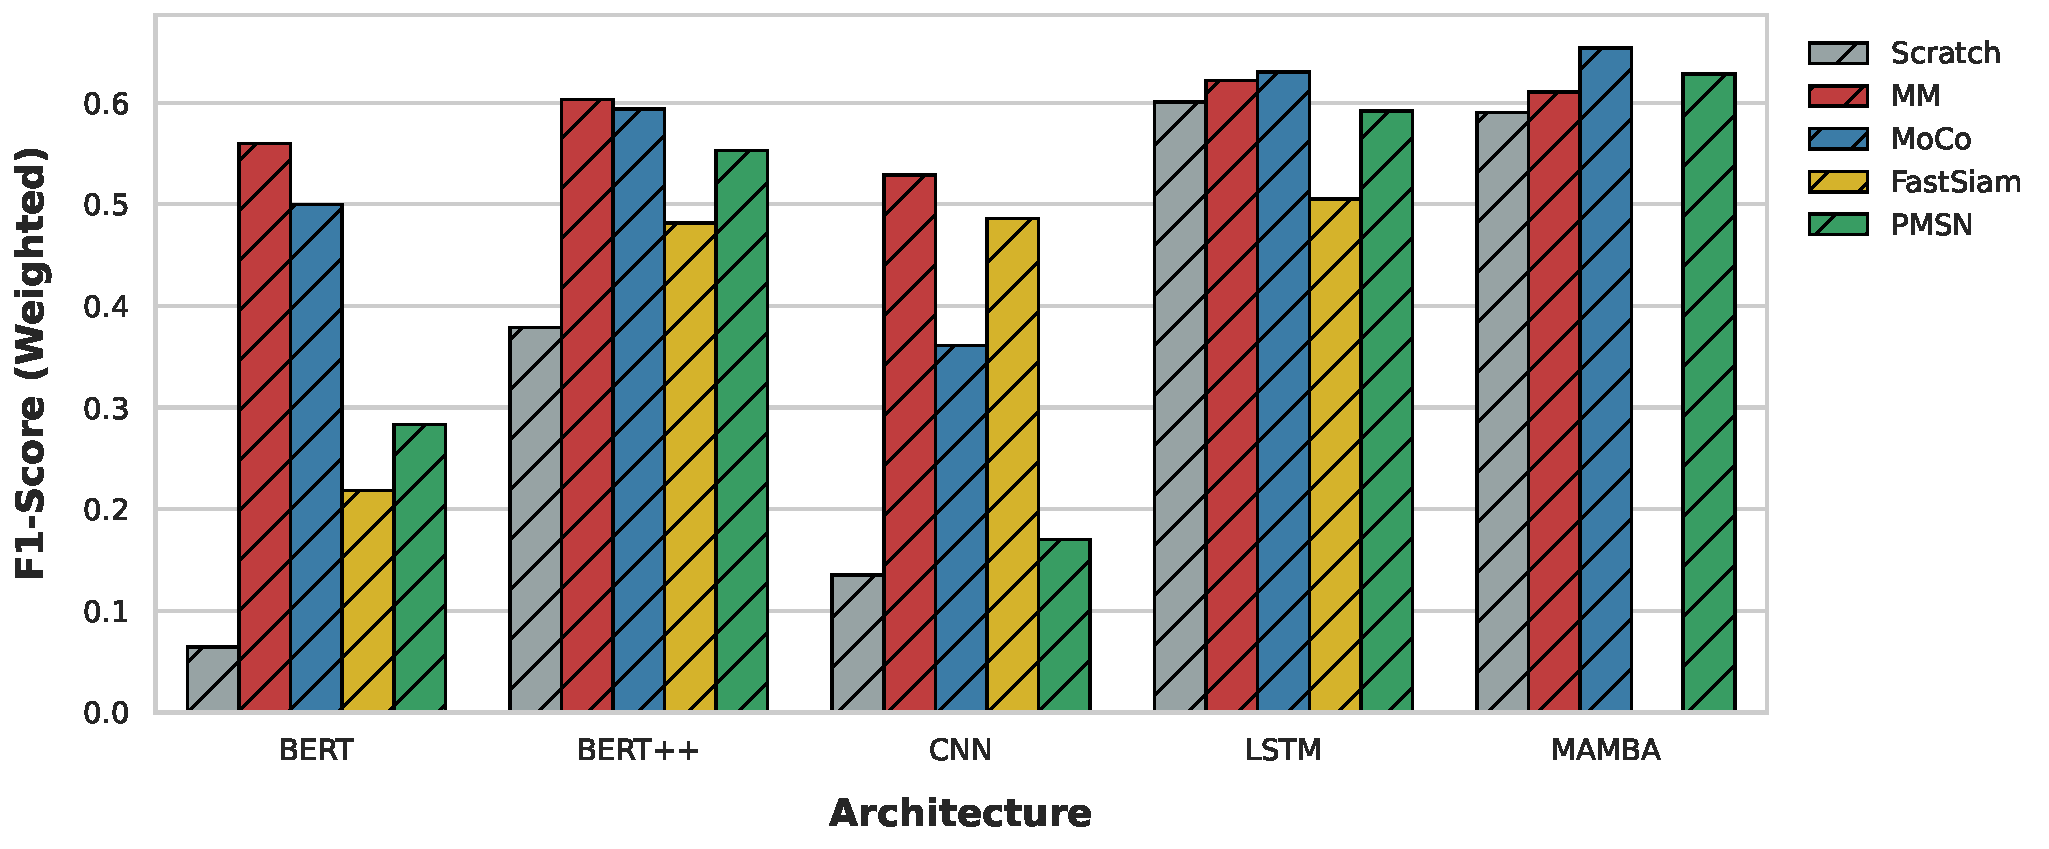
\includegraphics[width=0.7\linewidth]{figures/8_results/brazil-finetuning/few_shot_pretraining.pdf}
    \label{fig:fewshot_finetuning_few_brazil}
\end{figure}

\begin{figure}[ht!]
    \centering
    \caption{F1 Weighted of finetuning model per pretraining in few shot (0.1\% of training data) in California dataset.}
    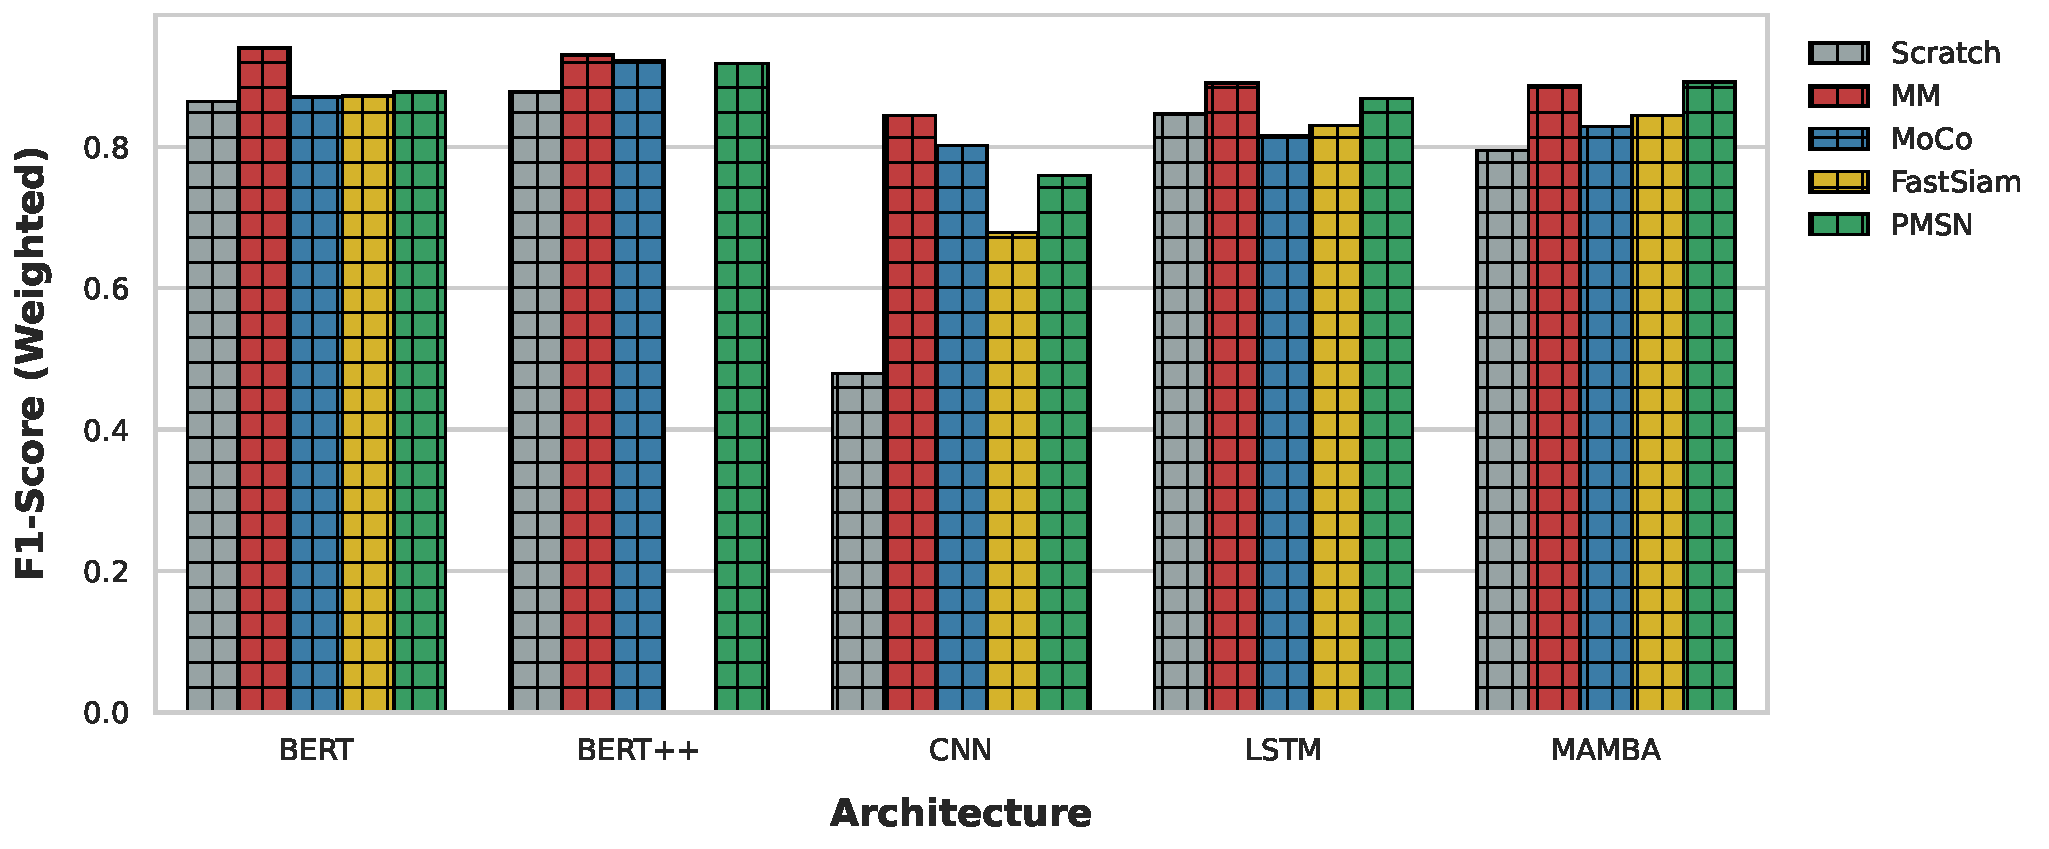
\includegraphics[width=0.7\linewidth]{figures/8_results/california-finetuning/few_shot_pretraining.pdf}
    \label{fig:fewshot_finetuning_few_california}
\end{figure}

\begin{figure}[ht!]
    \centering
    \caption{F1 Weighted of finetuning model per pretraining in few shot (0.1\% of training data) in Texas dataset.}
    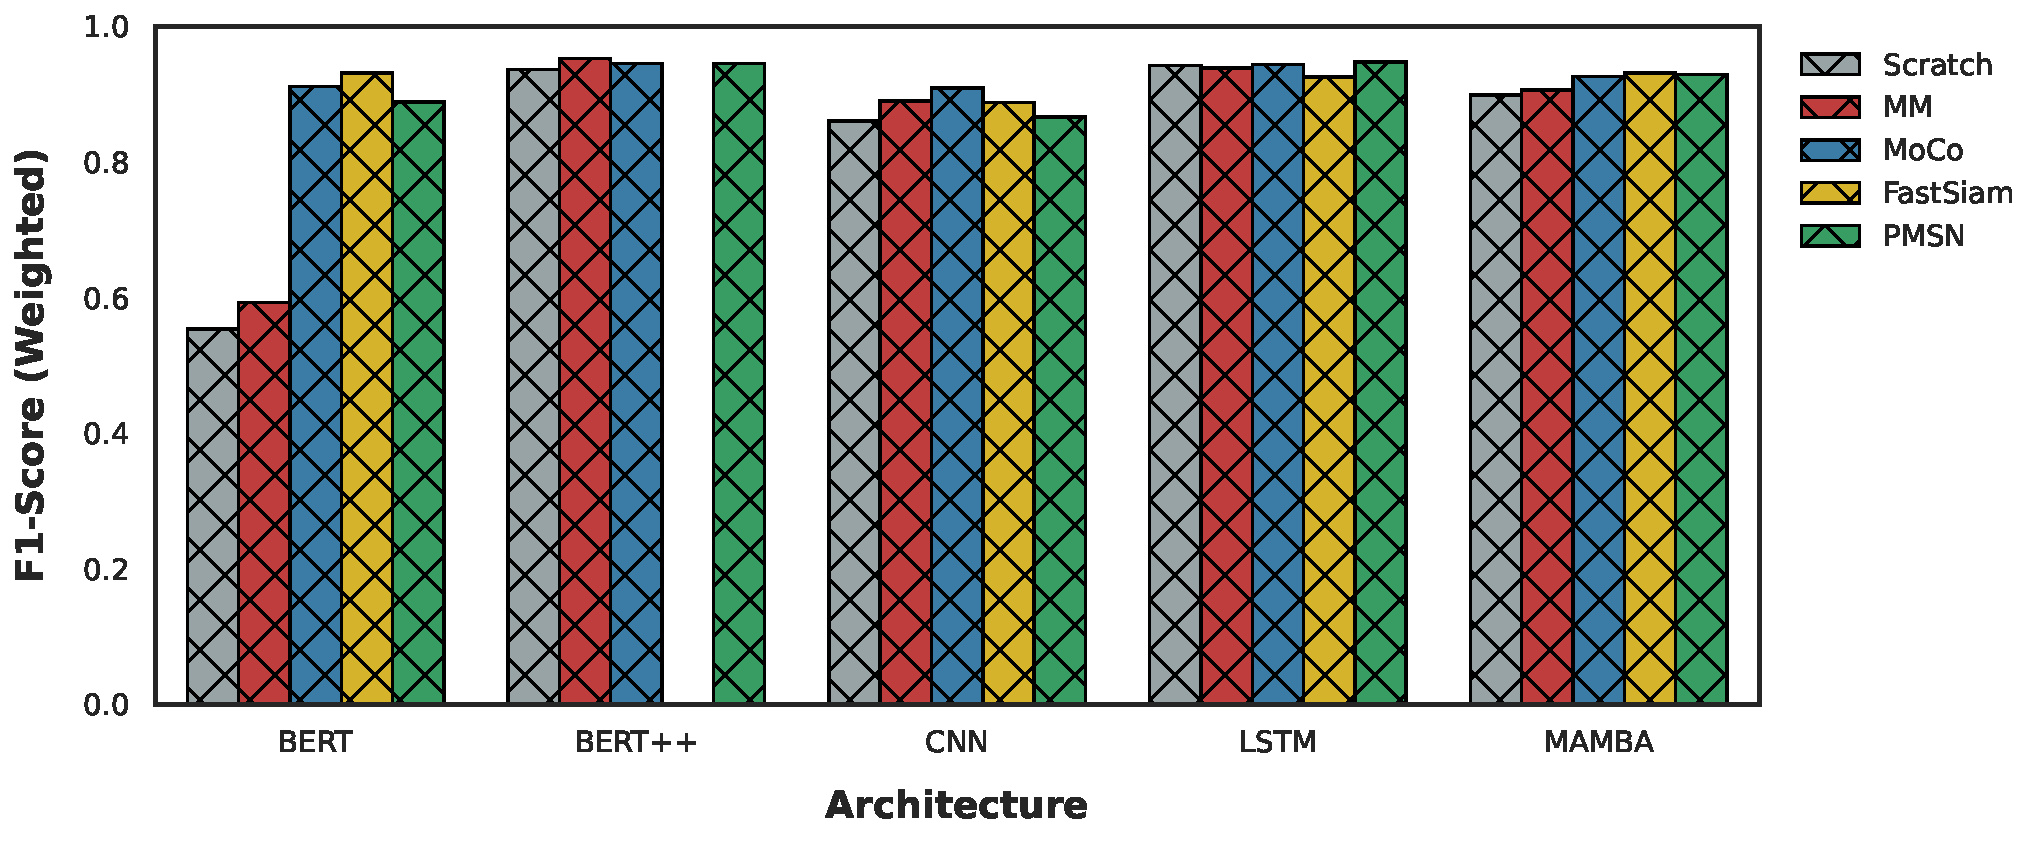
\includegraphics[width=0.7\linewidth]{figures/8_results/texas-finetuning/few_shot_pretraining.pdf}
    \label{fig:fewshot_finetuning_few_texas}
\end{figure}

In Brazil, the impact of pre-training is greater than that of other datasets (see Figure \ref{fig:fewshot_finetuning_few_brazil}). In scenarios with only 1\% of labeled data, models pre-trained with MoCo and MM significantly outperformed their from-scratch versions. SITS-BERT, for example, achieved gains of just over 21\% in F1 Weighted when using MoCo, and up to 40\% also with MoCo in SITS-CNN. These gains confirm that the internal representations learned during the self-supervised phase act as a powerful regularizer, preventing overfitting when labels are scarce. The model starts finetuning with a better initialization than random weights, which is crucial for the complex decision boundaries of the Brazil dataset. In this dataset and scenario, all pre-trainings showed some increase in the metric, with the most marginal being MM for SITS-Mamba, with less than 3\% gain. However, it is important to mention that this model, together with LSTM, already showed high results when compared to the others, even without pre-training.

In the California and Texas datasets (see Figures \ref{fig:fewshot_finetuning_few_california} and \ref{fig:fewshot_finetuning_few_texas}), the advantage of SSL is less noticeable, even in few-shot regimes. However, due to the apparent high separability of classes, even models trained from scratch tend to perform well, with the exceptions of the SITS-CNN models in California and SITS-BERT in Texas.

As for the impact of SSL pre-training on other data regimes, the gains are much smaller, although in very few cases there is a deterioration in performance due to pre-training. The convergence of the curves in Figures \ref{fig:fewshot_finetuning_brazil} through \ref{fig:fewshot_finetuning_texas} as the data percentage increases to 70\% (with enough labeled data), the supervised signal becomes strong enough to learn optimal features directly, rendering the pre-training initialization less critical. In addition, it is noteworthy that some models in some experiments generated unexpected results, indicating a poor fit. SITS-Mamba with MM in Brazil (see Figure \ref{fig:fewshot_finetuning_brazil}) showed a drop in performance when increasing the amount of labeled data from 1\% to 10\%, along with SVM in the same dataset. It is also noteworthy, analyzing the pre-training curves in relation to the shaded area of all datasets (see Figures \ref{fig:fewshot_finetuning_brazil}, \ref{fig:fewshot_finetuning_california}, and \ref{fig:fewshot_finetuning_texas}), that SITS-BERT and SITS-CNN are the models that most depend on pre-training, especially in few-shot scenarios, to present good results.

\begin{figure}[ht!]
    \centering
    \caption{F1 Weighted of finetuning model per pretraining in all data scarcity scenarios in Brazil dataset.}
    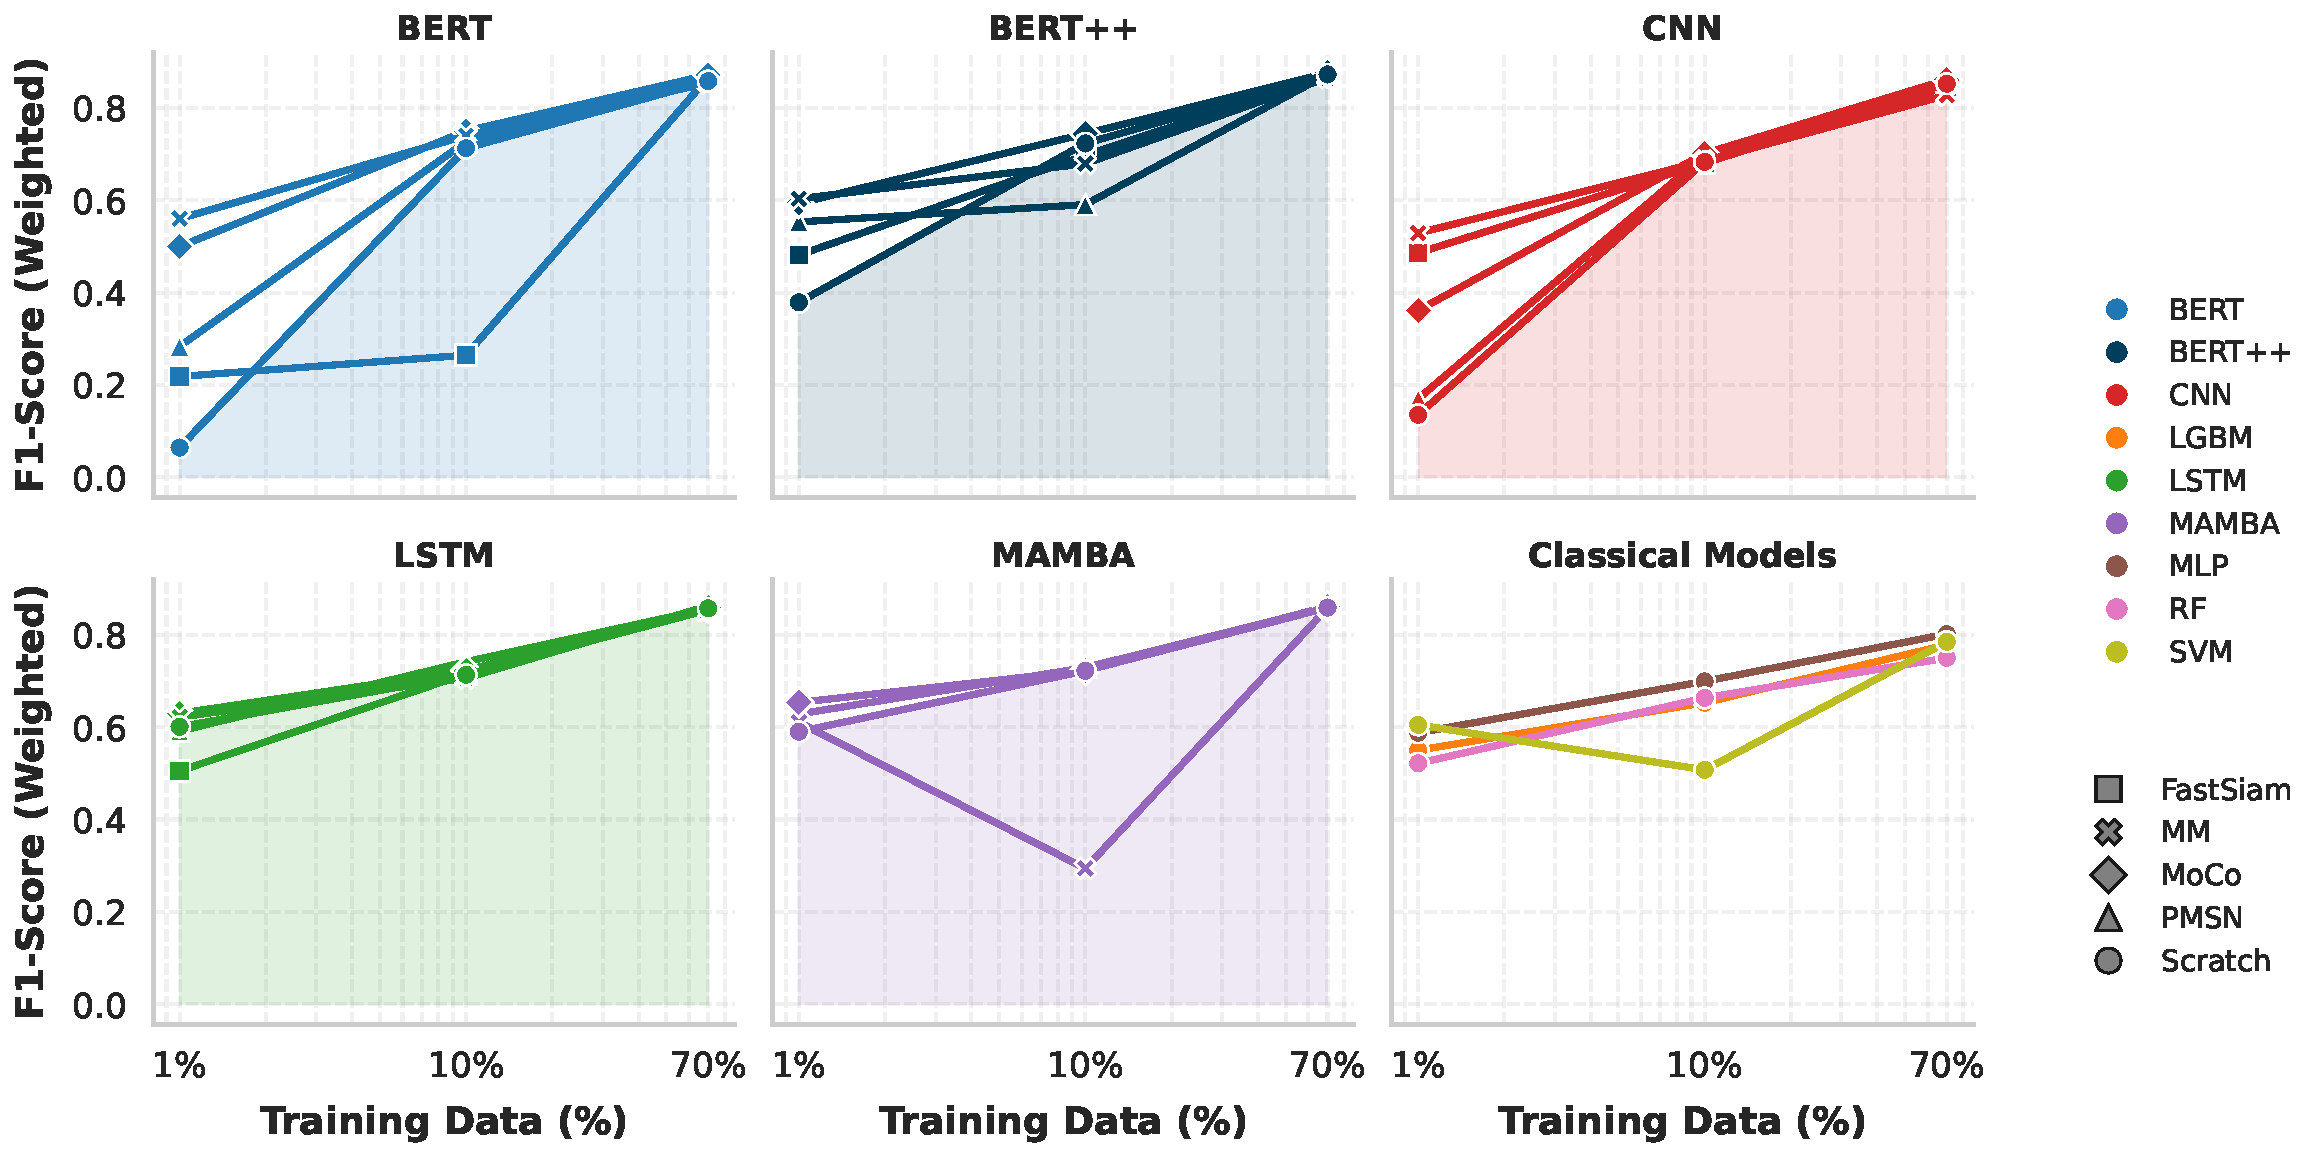
\includegraphics[width=0.7\linewidth]{figures/8_results/brazil-finetuning/line_training.pdf}
    \label{fig:fewshot_finetuning_brazil}
\end{figure}

\begin{figure}[ht!]
    \centering
    \caption{F1 Weighted of finetuning model per pretraining in all data scarcity scenarios in California dataset.}
    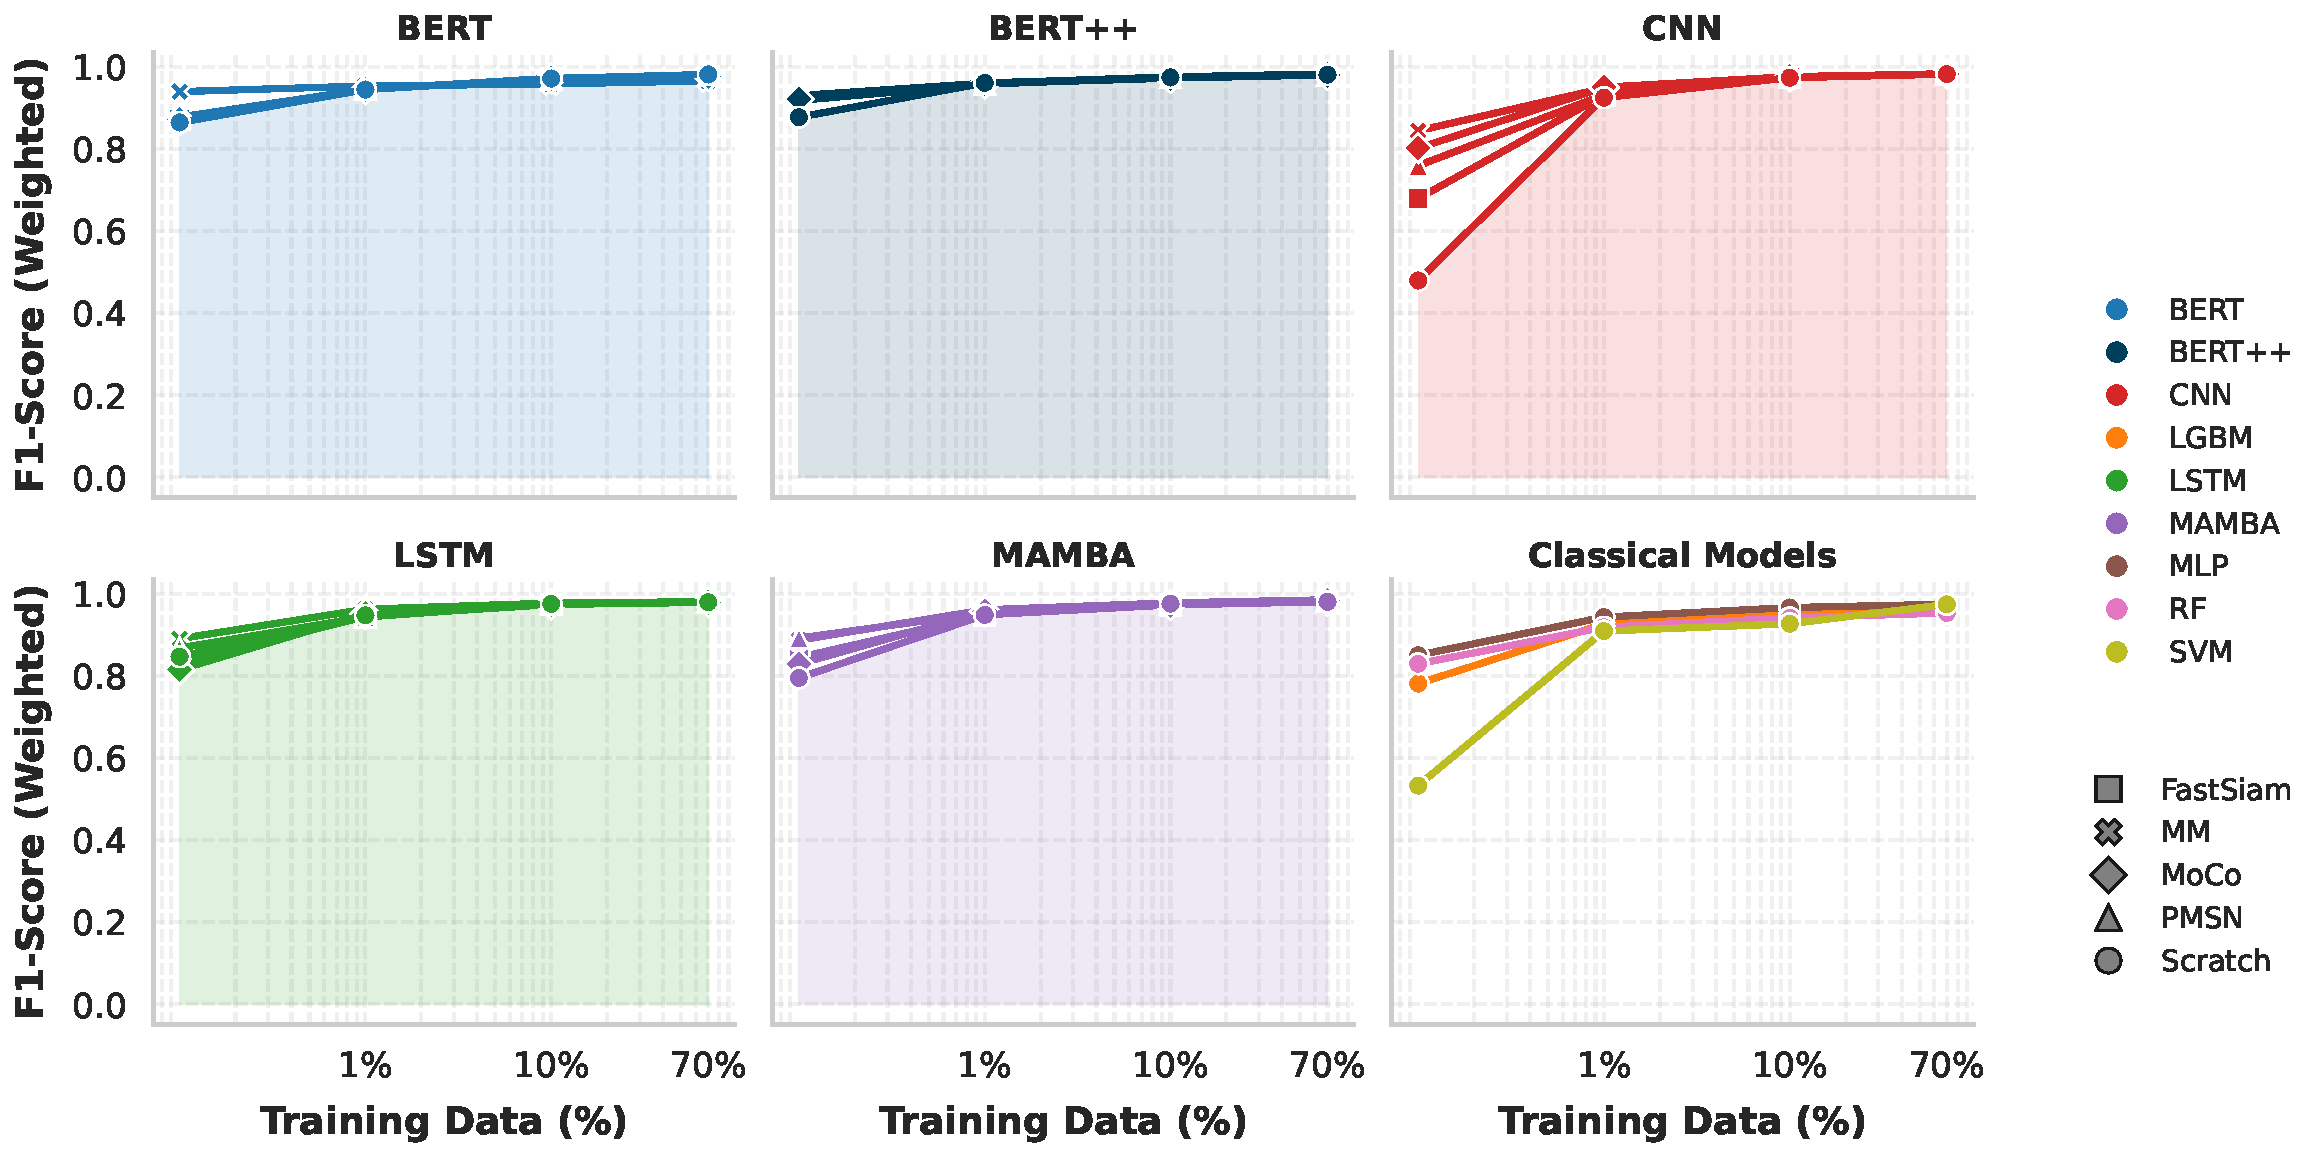
\includegraphics[width=0.7\linewidth]{figures/8_results/california-finetuning/line_training.pdf}
    \label{fig:fewshot_finetuning_california}
\end{figure}

\begin{figure}[ht!]
    \centering
    \caption{F1 Weighted of finetuning model per pretraining in all data scarcity scenarios in Texas dataset.}
    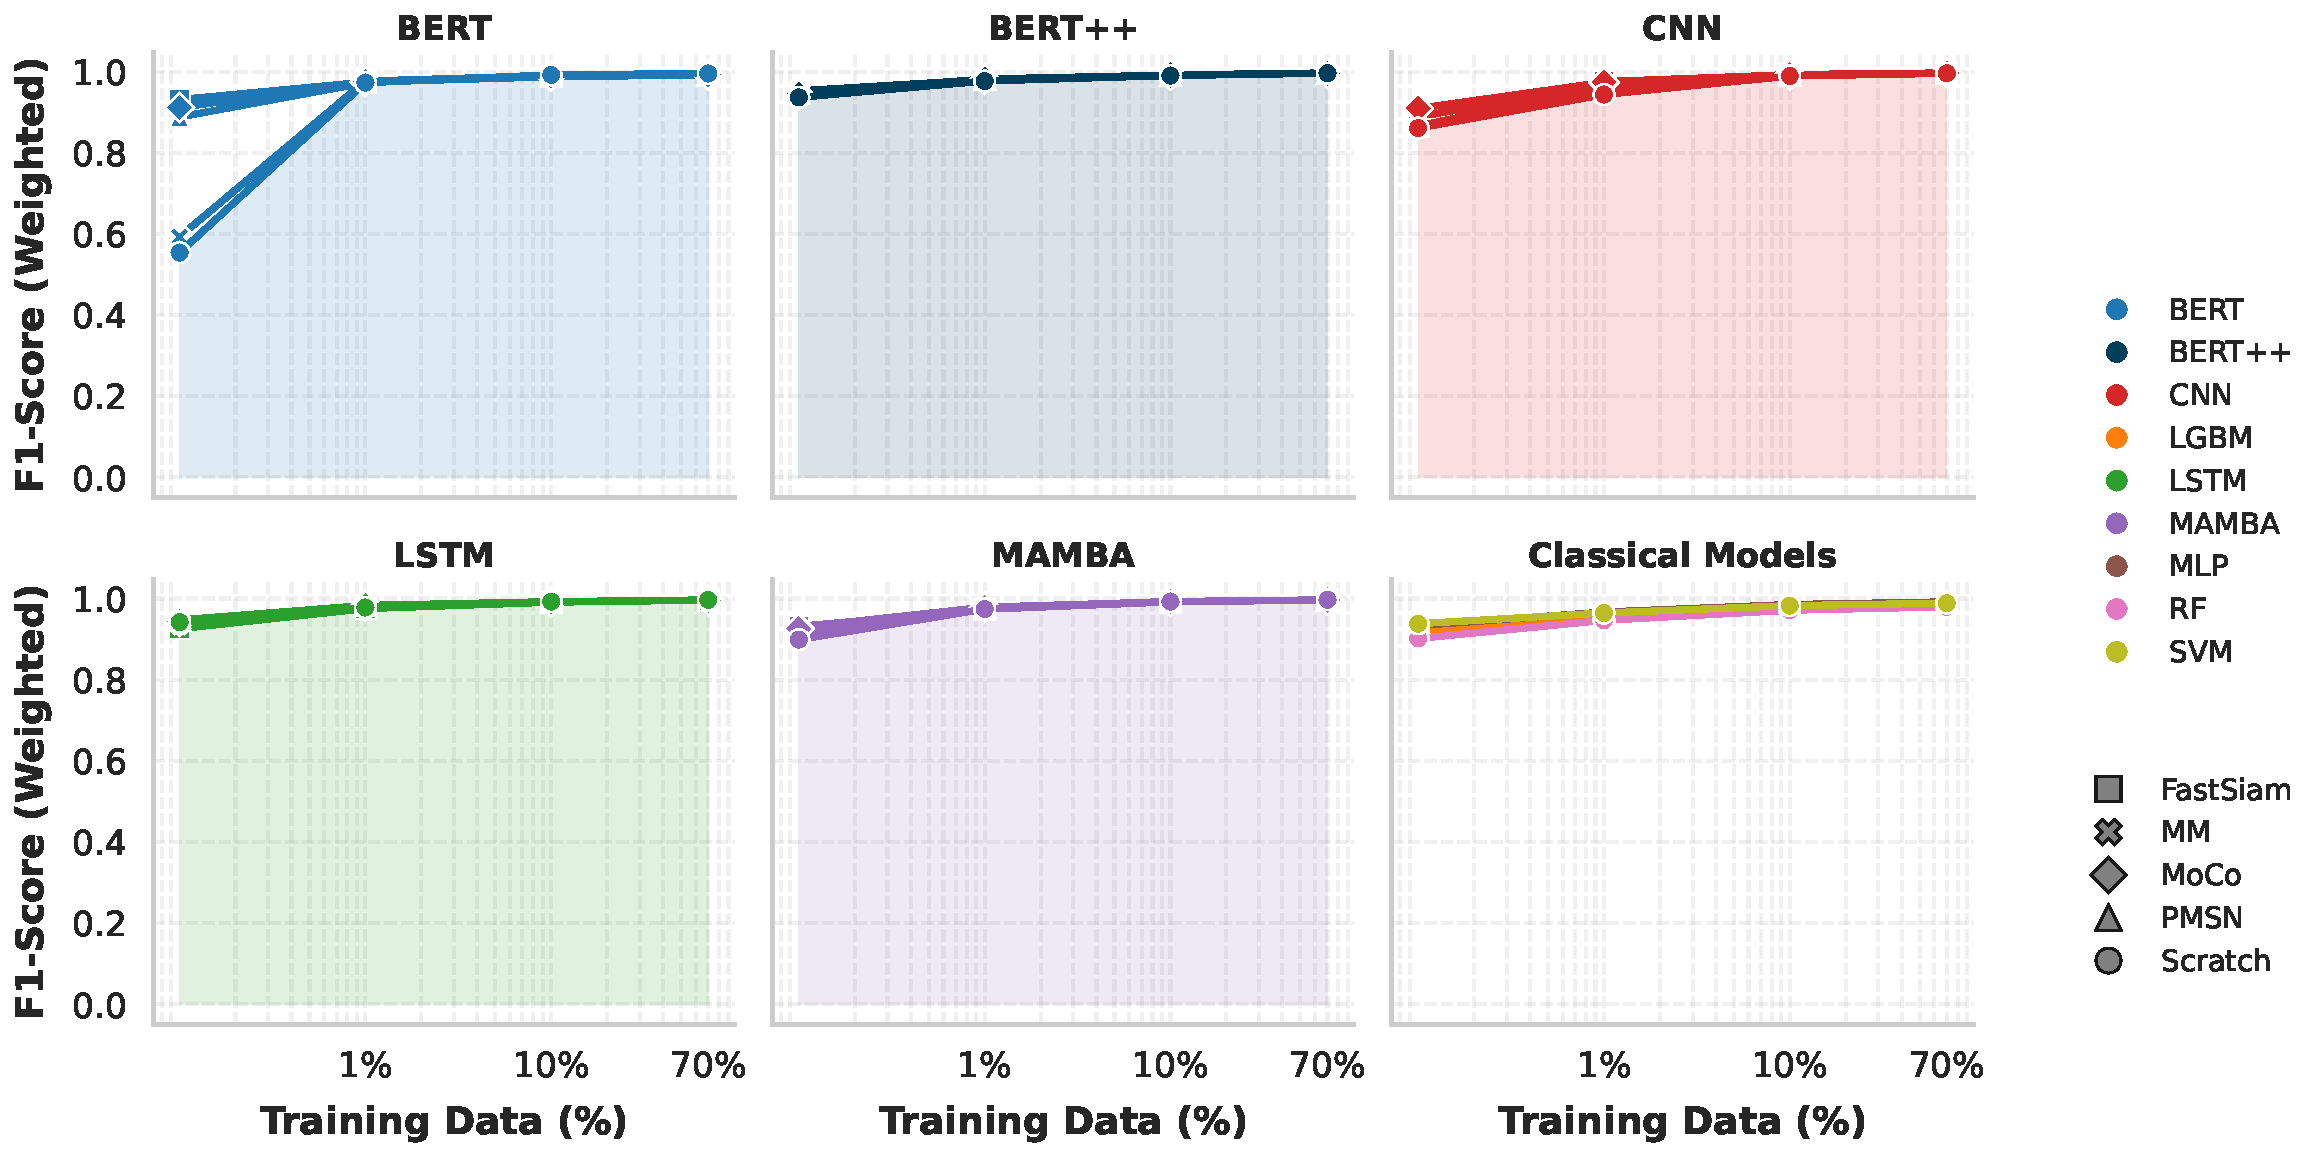
\includegraphics[width=0.7\linewidth]{figures/8_results/texas-finetuning/line_training.pdf}
    \label{fig:fewshot_finetuning_texas}
\end{figure}

\section{ORDER Anomaly Detection}

In the Brazil dataset (see Figure \ref{fig:trust_finetuning_brazil}), removing 5\% to 8\% of samples considered anomalous resulted in a consistent increase in performance (from around 84\% to around 88\% in some models), suggesting that ORDER was effective in identifying samples with noisy labels from Mapbiomas or plots with atypical spectral behavior. Furthermore, it is noticeable that MoCo pre-training identifies a similar number of anomalies even with a low percentage of removed samples when compared to PMSN or from scratch, indicating that the embeddings generated by MoCo are more robust and facilitate the detection of outliers.

\begin{figure}[ht!]
    \centering
    \caption{ORDER per model and pretraining in Brazil dataset.}
    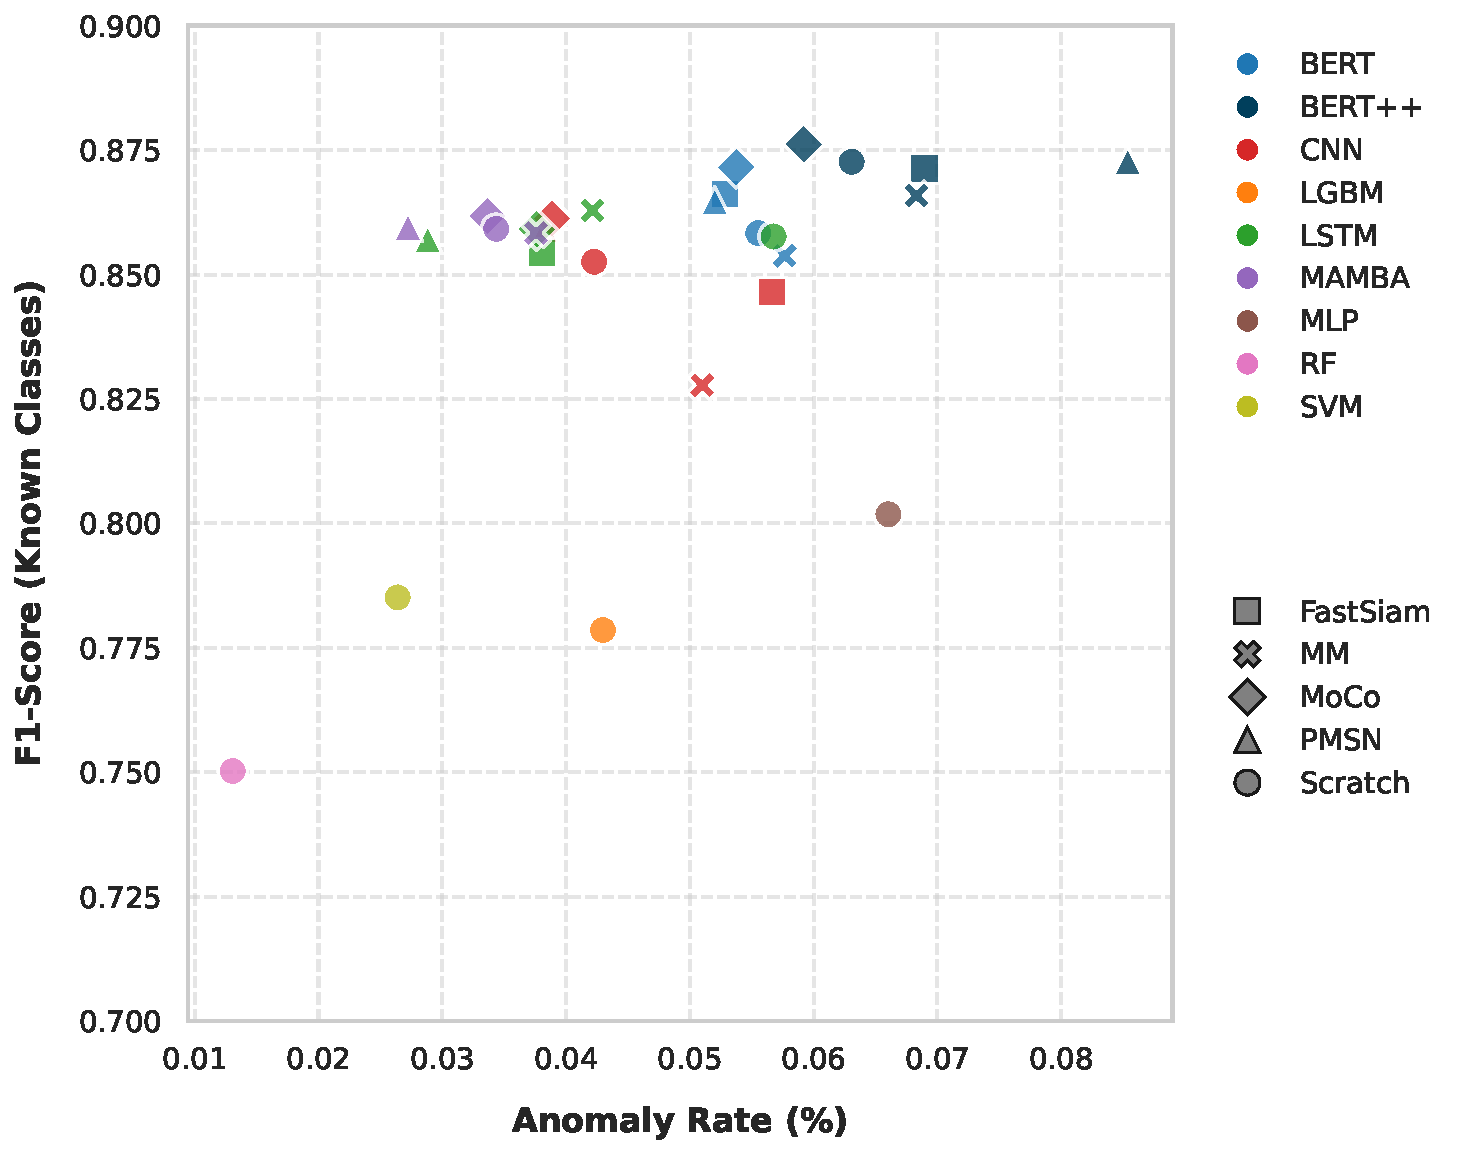
\includegraphics[width=0.6\linewidth]{figures/8_results/brazil-finetuning/trust_analysis.pdf}
    \label{fig:trust_finetuning_brazil}
    \fignote{The Y-axis starts at 0.7 and ends at 0.9.}
\end{figure}

\begin{figure}[ht!]
    \centering
    \caption{ORDER per model and pretraining in California dataset.}
    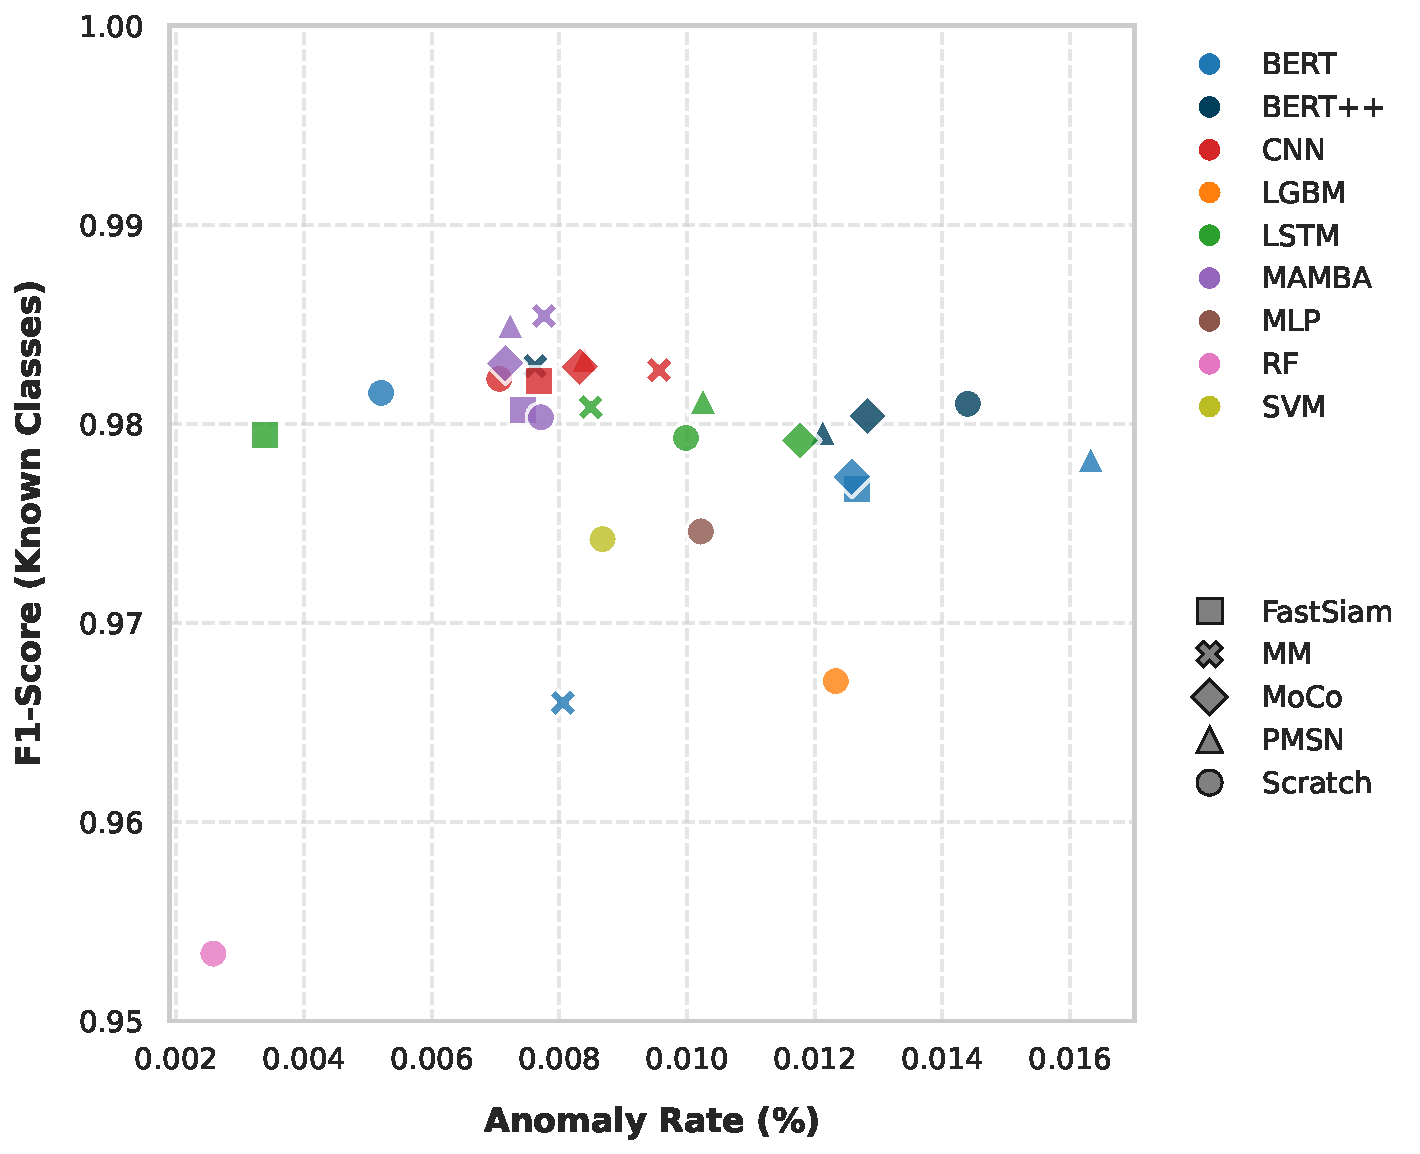
\includegraphics[width=0.6\linewidth]{figures/8_results/california-finetuning/trust_analysis.pdf}
    \label{fig:trust_finetuning_california}
    \fignote{The Y-axis starts at 0.9 and ends at 1.0.}
\end{figure}

\begin{figure}[ht!]
    \centering
    \caption{ORDER per model and pretraining in Texas dataset.}
    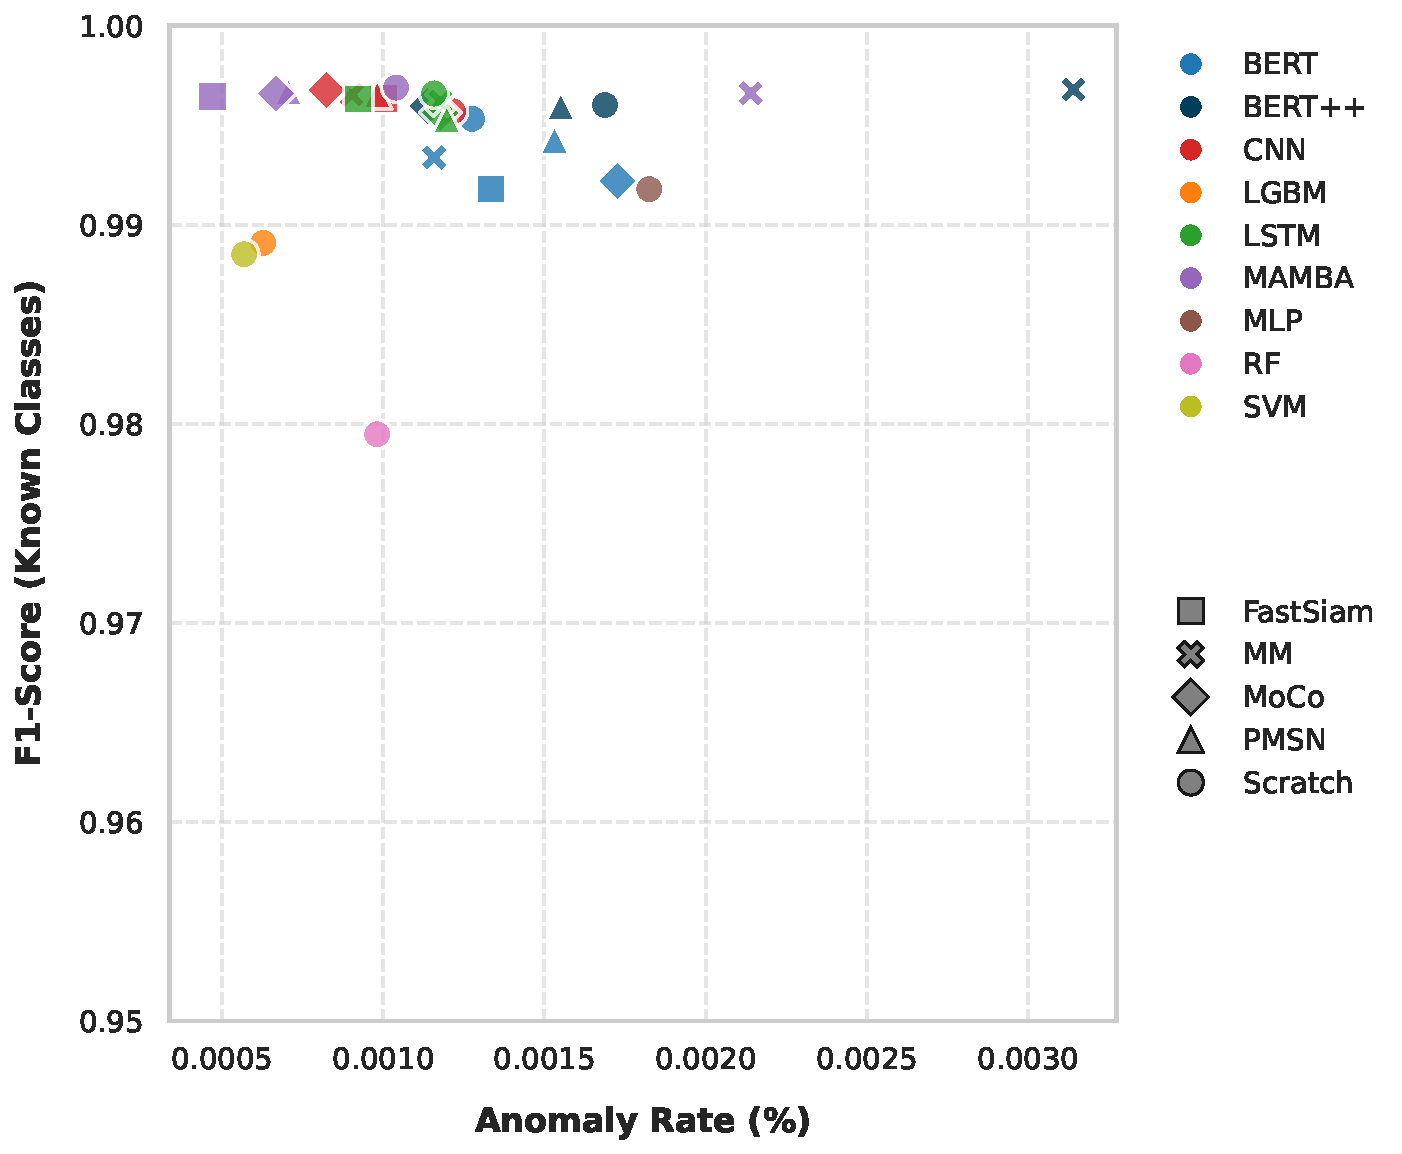
\includegraphics[width=0.6\linewidth]{figures/8_results/texas-finetuning/trust_analysis.pdf}
    \label{fig:trust_finetuning_texas}
    \fignote{The Y-axis starts at 0.9 and ends at 1.0.}
\end{figure}

Conversely, for the California and Texas datasets (see Figures \ref{fig:trust_finetuning_california} and \ref{fig:trust_finetuning_texas}), the improvements were more modest, primarily due to the performance saturation where baseline metrics already exceeded 98\%. However, a crucial finding is the stability of the ORDER framework in these high-accuracy regimes. Unlike traditional uncertainty filtering, which often degrades performance in well-separated data by discarding informative hard samples, ORDER maintained metric stability or provided marginal gains. This behavior indicates that the method is selective and conservative, targeting genuine label noise rather than merely removing difficult examples, essentially acting as a safe filter that preserves the decision boundary integrity even when the anomaly rate is naturally low.

\section{Best results per dataset}

This section details the best experiment obtained for each dataset, analyzing the confusion matrices, the distribution of embeddings using t-SNE dimensionality reduction, and verifying the separability between correct and incorrect predictions using the model itself, ConfidNet, and the proposed ORDER method.

\subsection{Brazil Dataset}

\begin{figure}[ht!]
    \centering
    % Início da primeira subfigura (Matriz)
    \begin{subfigure}[b]{0.48\textwidth}
        \centering
        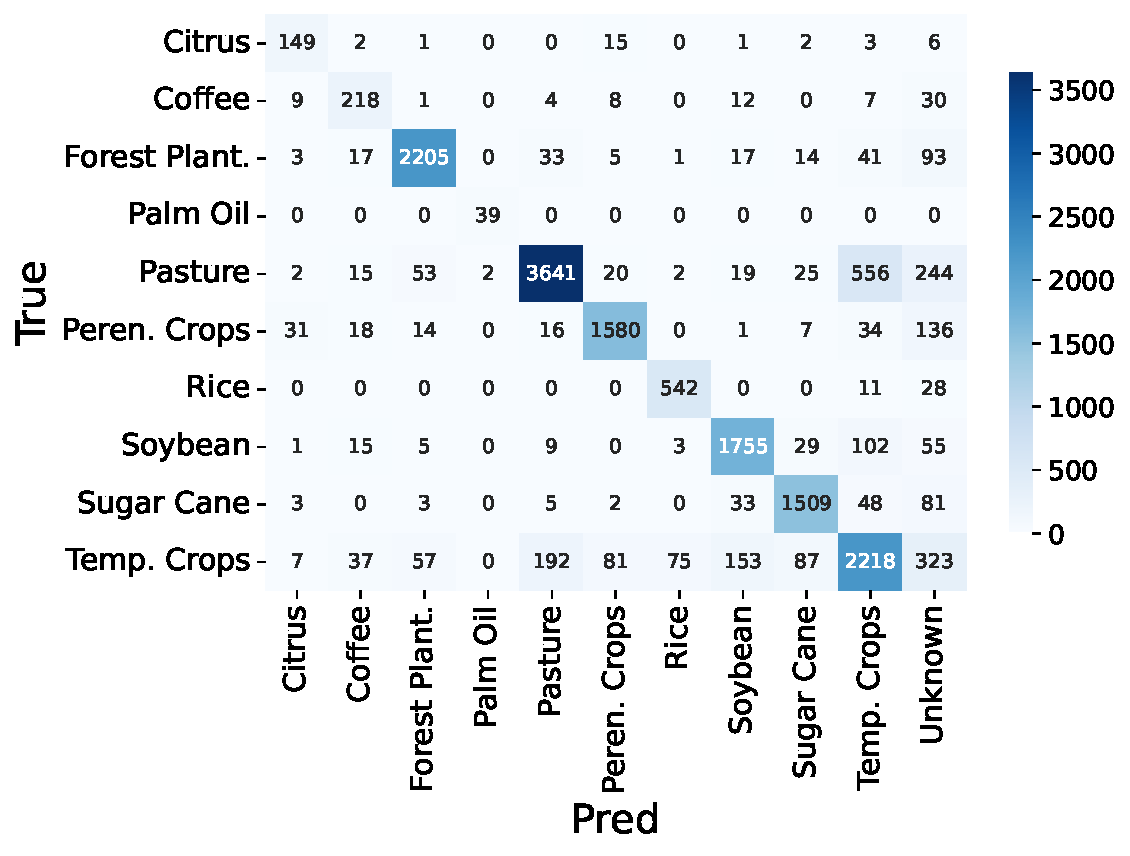
\includegraphics[width=\linewidth]{figures/8_results/brazil-finetuning/BERTPP-70.0-MoCo/class_test_gemmos_matrix.pdf}
        %\caption{Matriz de Confusão}
        \label{fig:brazil_cm}
    \end{subfigure}
    \hfill % Adiciona espaço elástico entre as figuras
    % Início da segunda subfigura (Relatório)
    \begin{subfigure}[b]{0.48\textwidth}
        \centering
        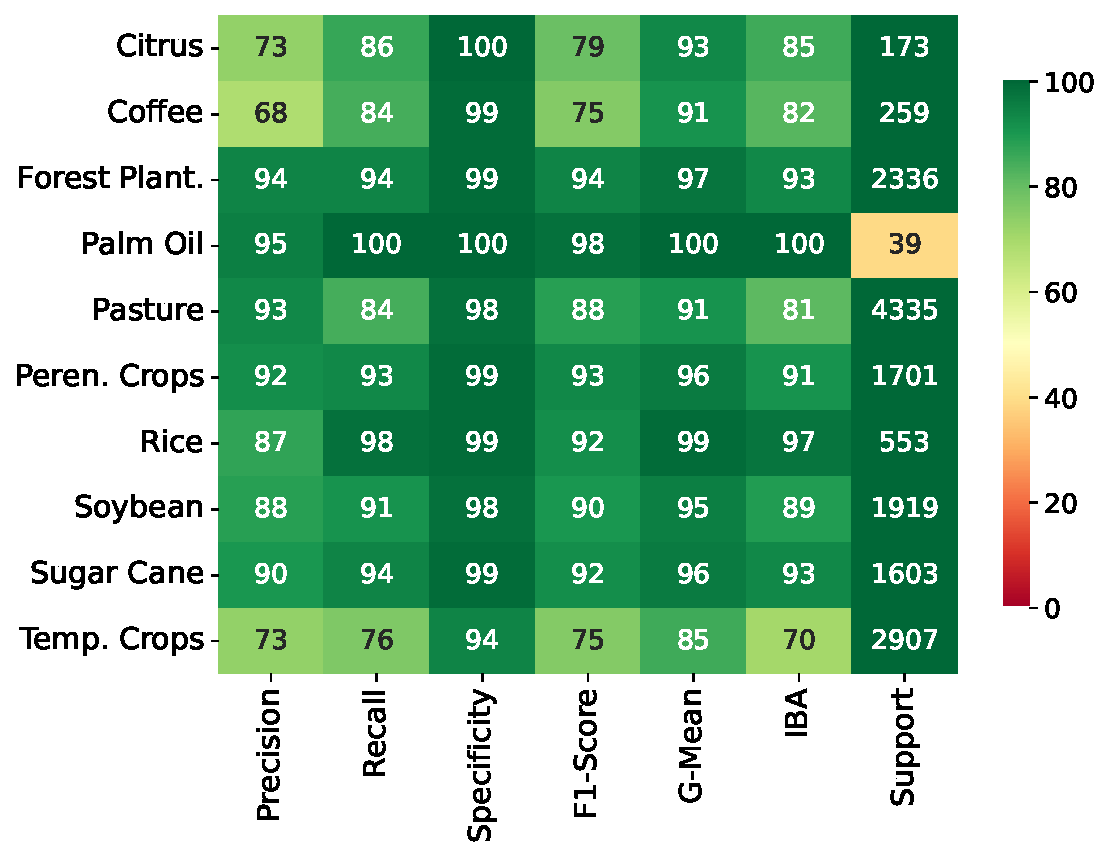
\includegraphics[width=\linewidth]{figures/8_results/brazil-finetuning/BERTPP-70.0-MoCo/class_test_gemmos_report.pdf}
        %\caption{Relatório de Classificação}
        \label{fig:brazil_cr}
    \end{subfigure}
    
    % Legenda geral para ambas as figuras
    \caption{Best experiment in Brazil Dataset class. Report with 70\% in training data (BERT++ with MoCo pretraining).}
    \label{fig:brazil_experiments}
\end{figure}

A closer look of the results from the best experiment on the Brazilian (see \autoref{fig:brazil_experiments}) dataset reveals that the confusion matrix has a significantly high main diagonal, indicating that the model has a high accuracy rate in correctly classifying the classes. The most problematic classes are Pasture, Temporary Crops, and Perennial Crops. The Pasture class is quite complex due to seasonal variations and different agricultural practices that affect its appearance in the SITS, in addition to being more affected by rainfall. The Temporary Crops and Perennial Crops classes, in turn, can contain a variety of crops with different growth cycles, which can lead to classification confusion, and may even include other classes present in the dataset. The \ac{ORDER} method rejects more true samples precisely in these classes, indicating its effectiveness, even in a scenario of high model metrics, where the ConfidNet baseline tends not to perform well.

The evaluation metrics in the classification report confirm the robustness of the framework, with Specificity and G-Mean metrics exceeding 90\% for most categories. However, the Other Temporary Crops and Other Perennial Crops classes show the lowest IBA indices (70 and 91, respectively) and slightly reduced F1-Score metrics when compared to more stable classes, such as Palm Oil and Rice.

\begin{figure}[ht!]
    \centering
    \caption{Best experiment in Brazil Dataset with 70\% in training data (BERT++ with MoCo pretraining) separability between right and wrong predictions with ORDER, ConfidNet and MCP.}
    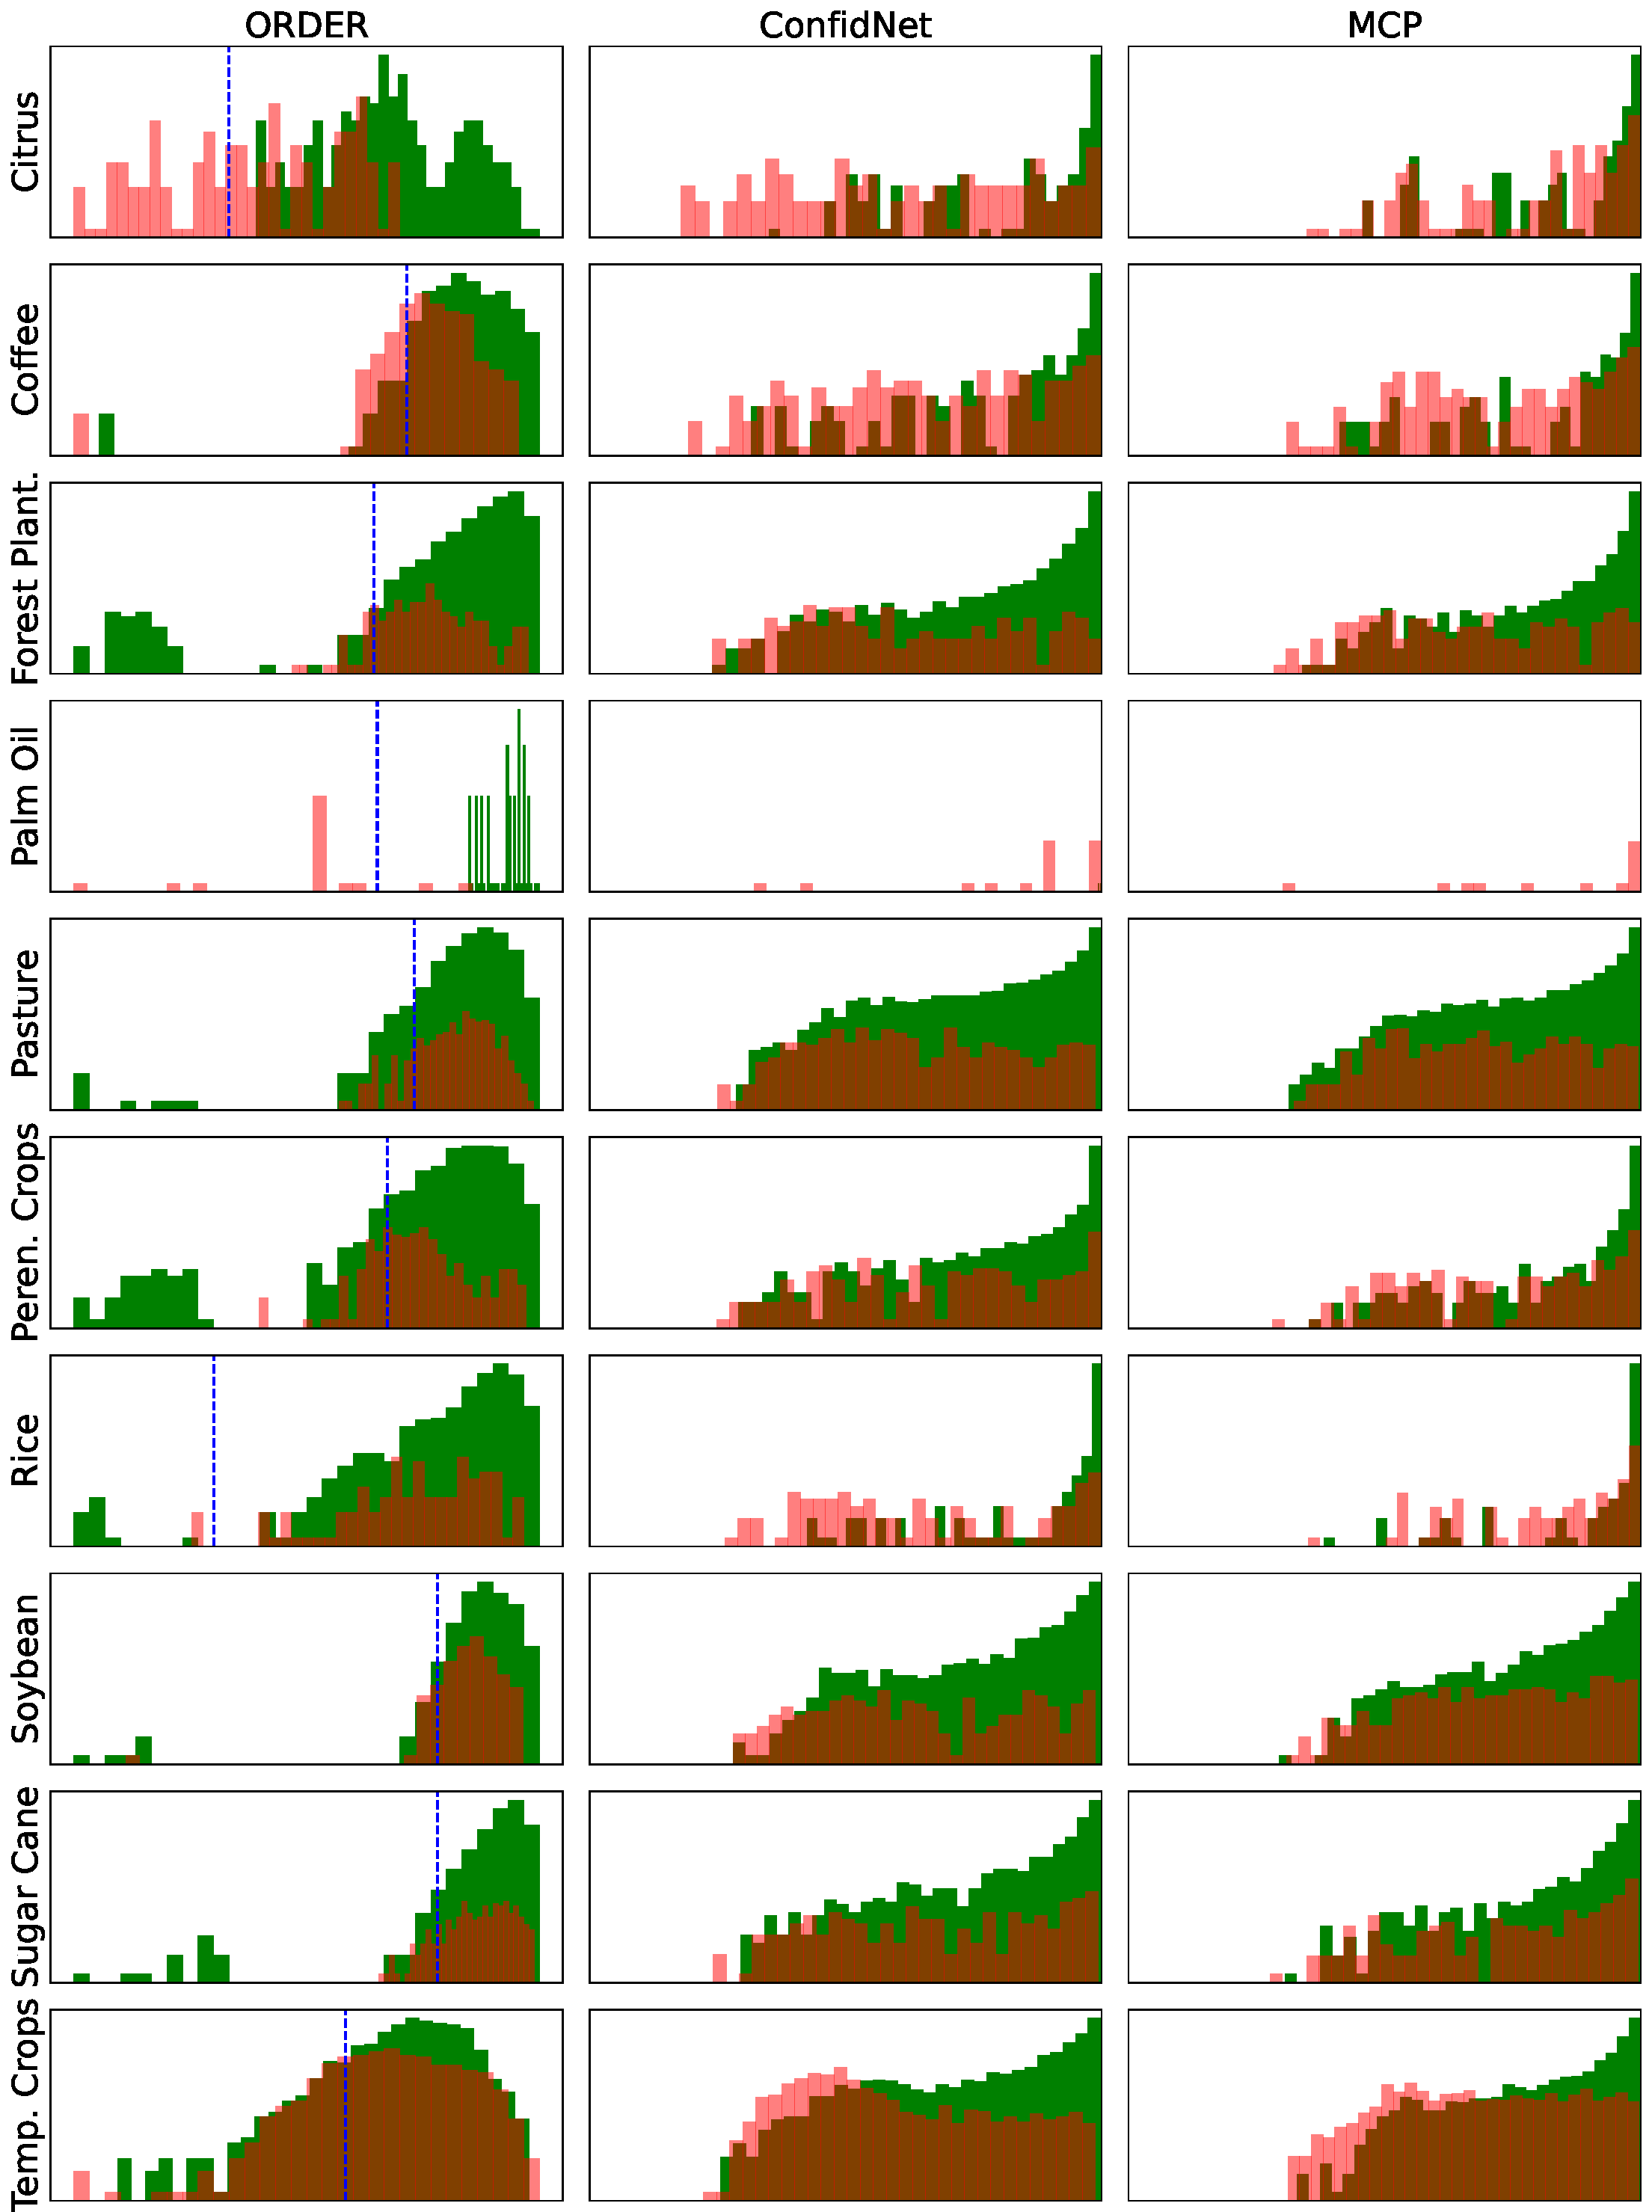
\includegraphics[width=0.6\linewidth]{figures/8_results/brazil-finetuning/BERTPP-70.0-MoCo/hist_combined_test.pdf}
    \label{fig:brazil_gmm}
    \fignote{Y-axis is in logarithmic scale.}
\end{figure}

The histograms illustrate the superiority of ORDER in separating correct from incorrect predictions (see \autoref{fig:brazil_gmm}). While ConfidNet and the Model Confidence show overlapping distributions (Right and Wrong predictions both clustering near high confidence values, being overconfident), the \ac{ORDER} method exhibits a clearer bimodal separation. This separation allows for a more effective thresholding strategy to filter out potential errors without discarding too many correct predictions.

\subsection{Texas Dataset}

\begin{figure}[ht!]
    \centering
    % Início da primeira subfigura (Matriz)
    \begin{subfigure}[b]{0.48\textwidth}
        \centering
        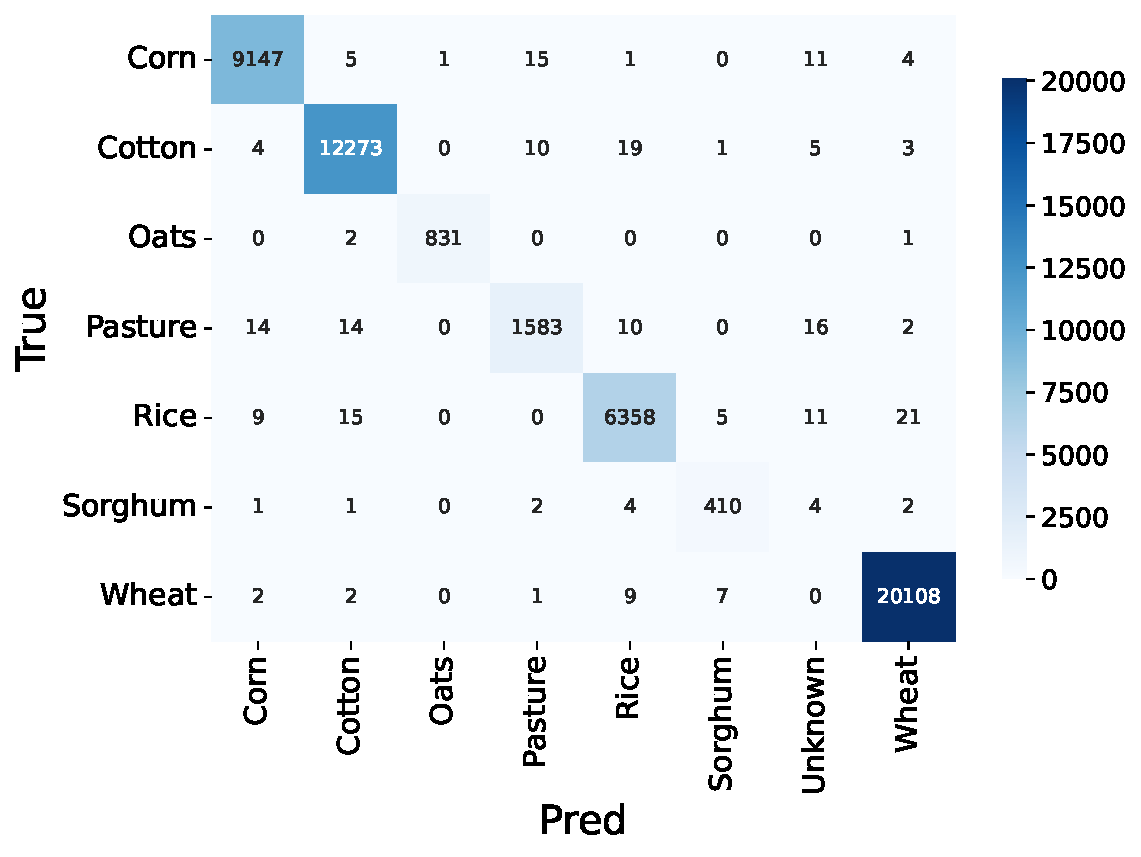
\includegraphics[width=\linewidth]{figures/8_results/texas-finetuning/LSTM-70.0-FastSiam/class_test_gemmos_matrix.pdf}
        %\caption{Matriz de Confusão}
        \label{fig:texas_cm}
    \end{subfigure}
    \hfill % Adiciona espaço elástico entre as figuras
    % Início da segunda subfigura (Relatório)
    \begin{subfigure}[b]{0.48\textwidth}
        \centering
        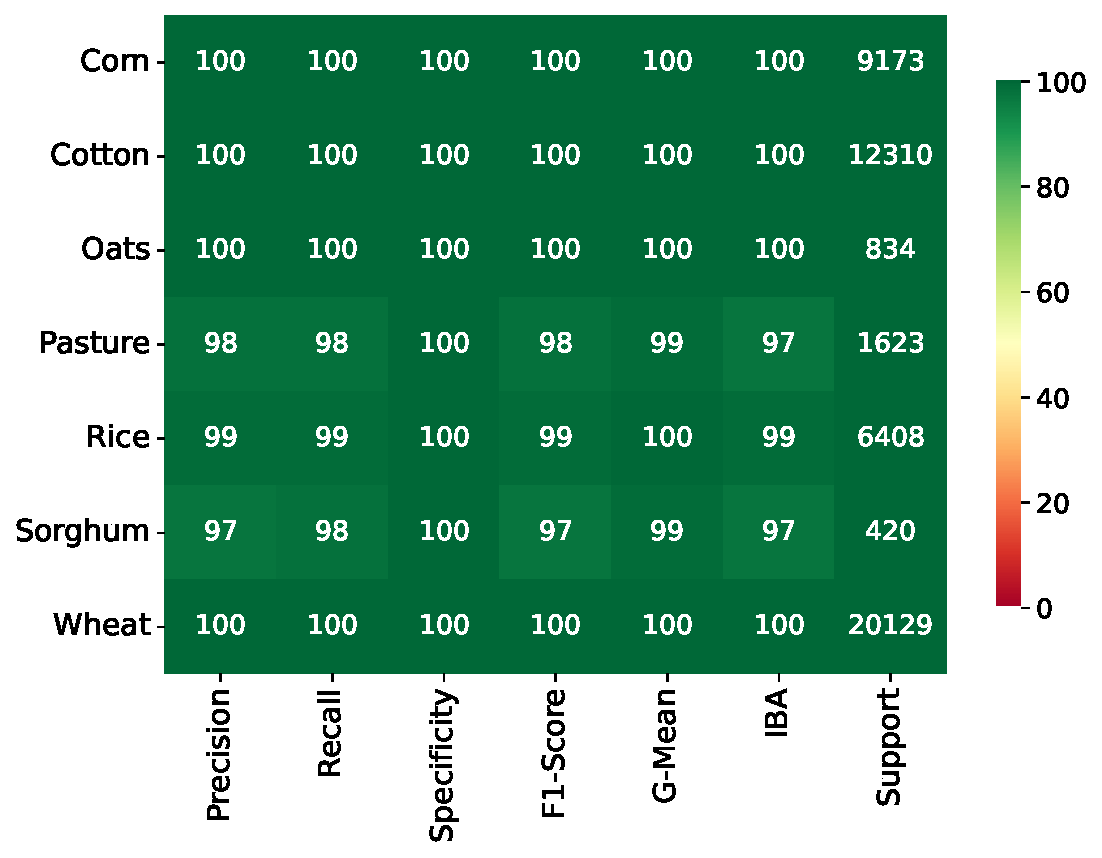
\includegraphics[width=\linewidth]{figures/8_results/texas-finetuning/LSTM-70.0-FastSiam/class_test_gemmos_report.pdf}
        %\caption{Relatório de Classificação}
        \label{fig:texas_cr}
    \end{subfigure}
    
    % Legenda geral para ambas as figuras
    \caption{Best experiment in Texas Dataset with 70\% in training data (LSTM with FastSiam pretraining).}
    \label{fig:texas_experiments}
\end{figure}

Doing the same with the Texas dataset (see \autoref{fig:texas_experiments}), the best experiment on this dataset was using the LSTM model with FastSiam pretraining, revealing  high performance. The confusion matrix shows an extremely clean main diagonal, indicating that the model achieved near-perfect separation for classes such as Corn, Cotton, and Wheat, with hits exceeding 9,000, 12,000, and 20,000 instances, respectively. The reduced incidence of values in the ``Unknown'' column suggests that, in this dataset, the ORDER method found fewer anomalies, which may be attributed to a database with less noisy labels or to a greater spectral-temporal distinction between Texas agricultural crops compared to Brazilian ones.

\begin{figure}[ht!]
    \centering
    \caption{Best experiment in Texas Dataset with 70\% in training data (LSTM with FastSiam pretraining) separability between right and wrong predictions with ORDER, ConfidNet and MCP.}
    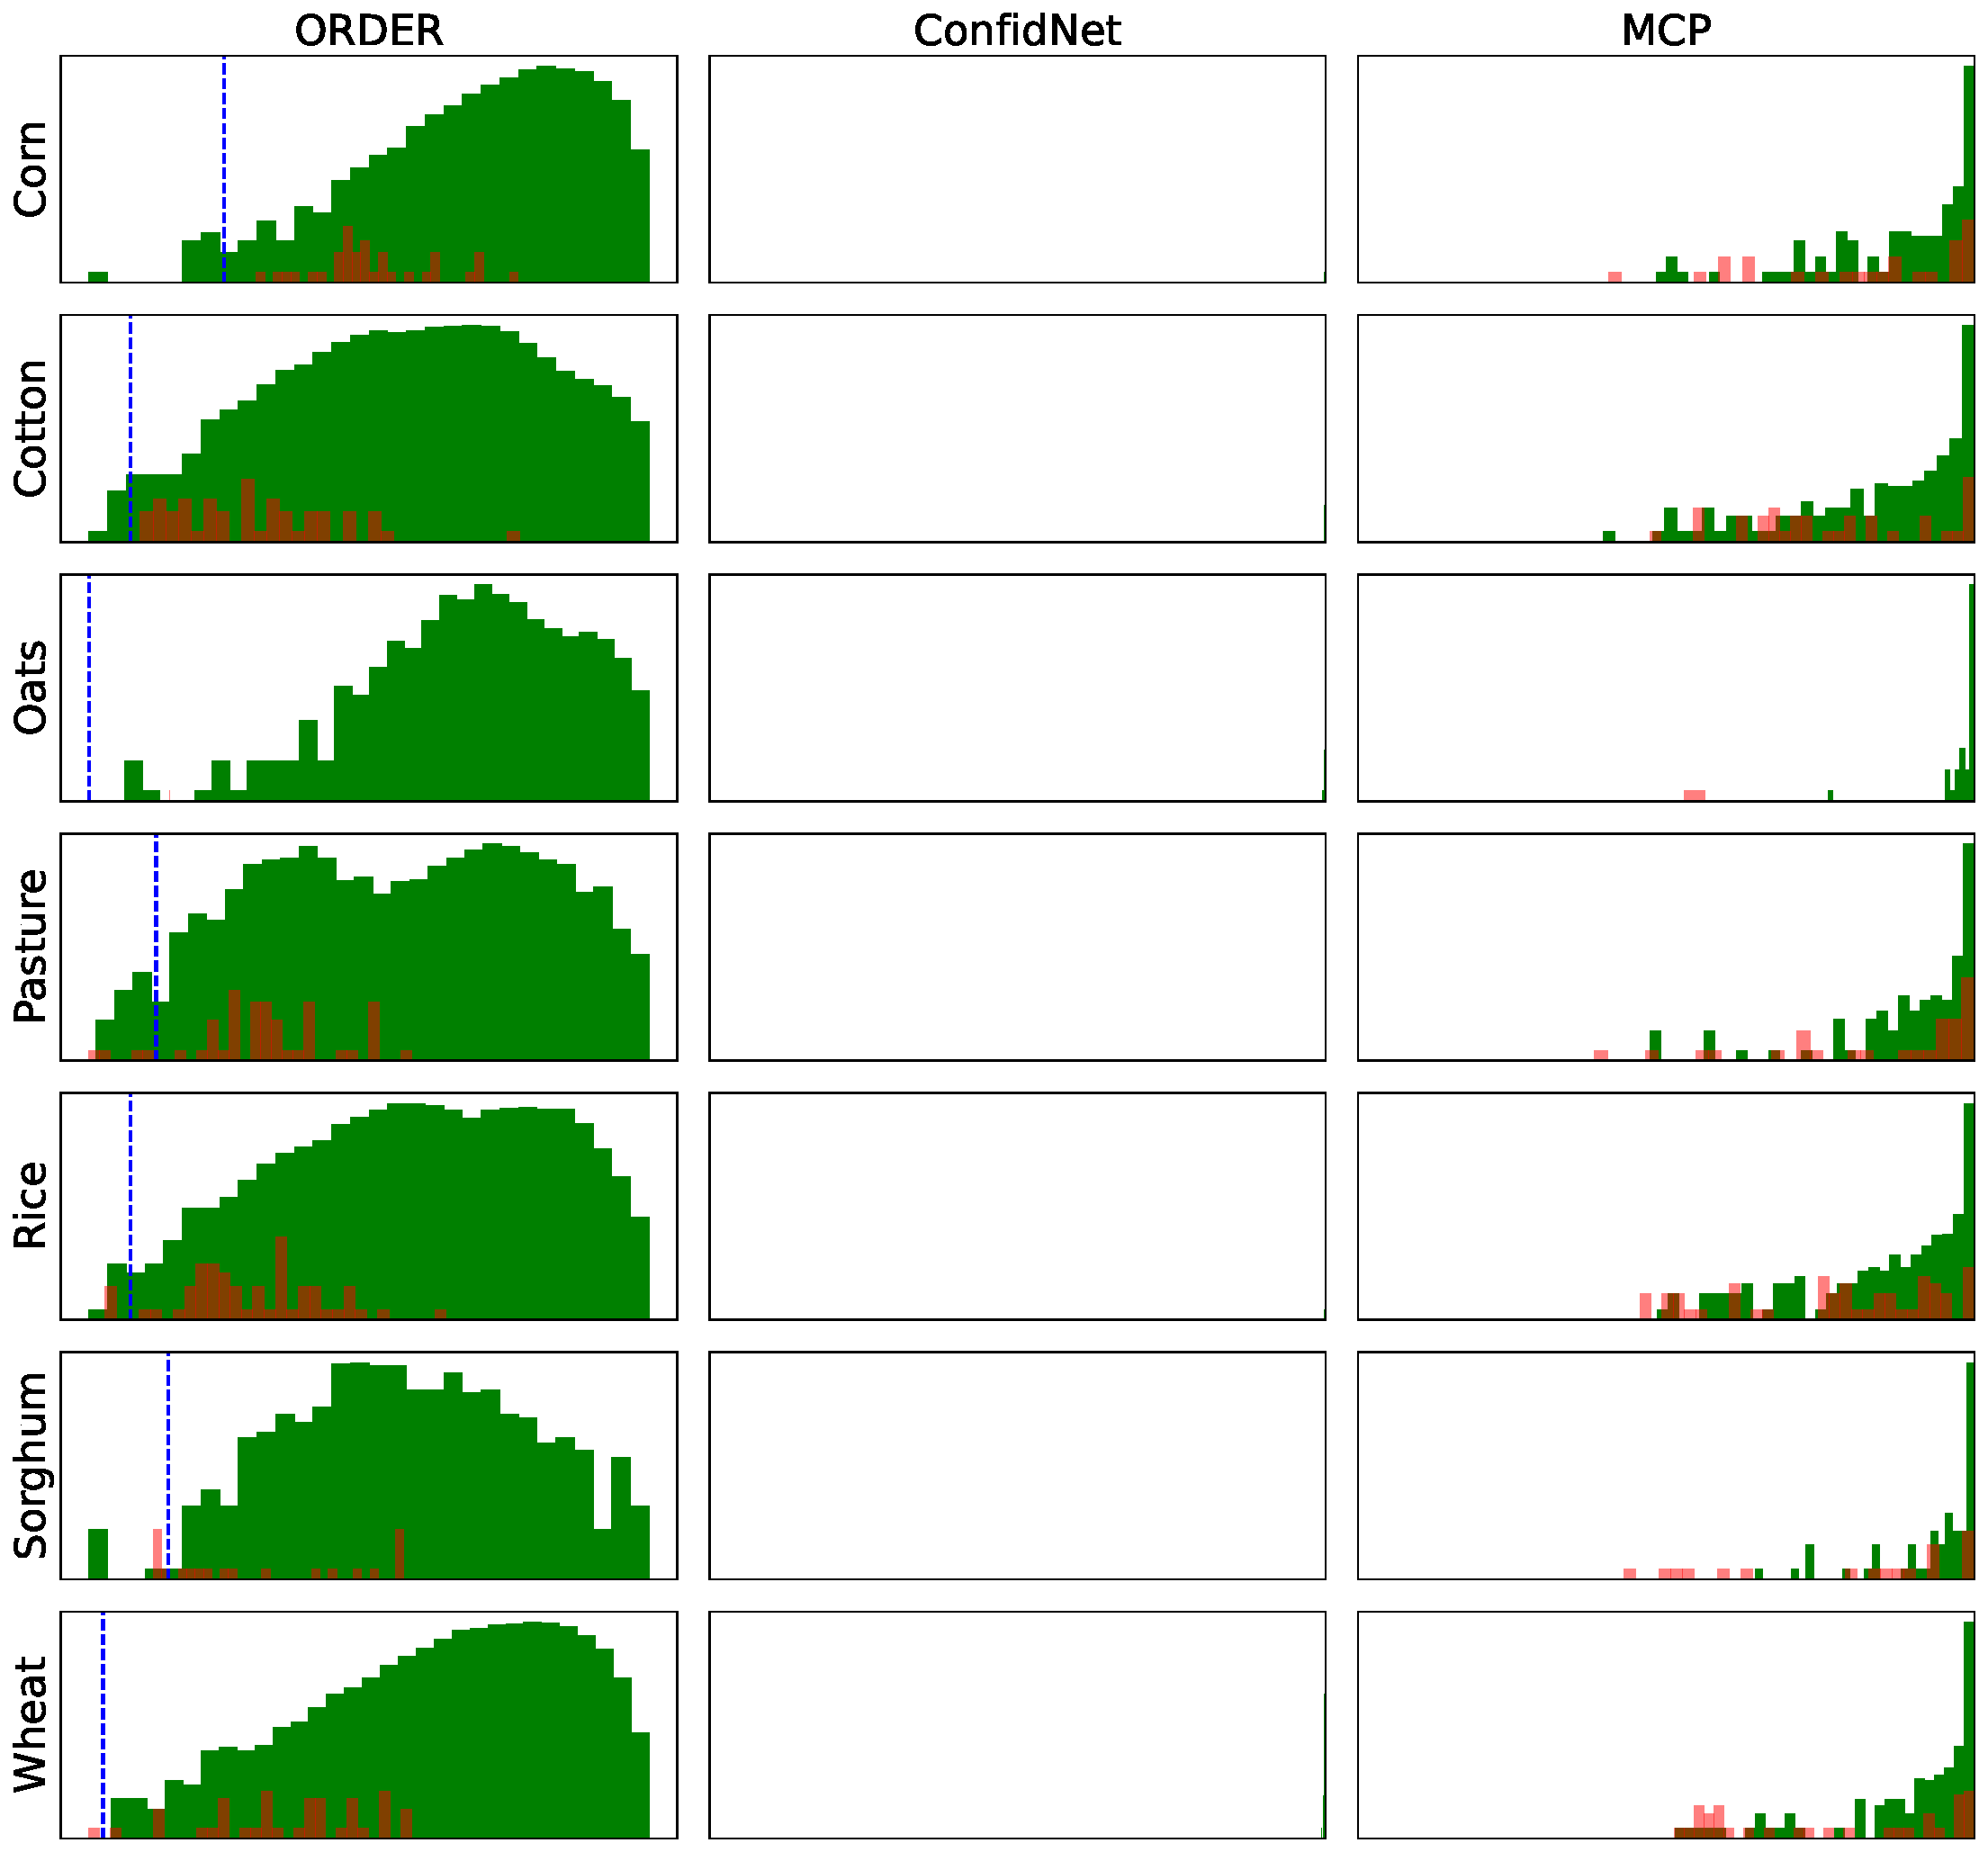
\includegraphics[width=0.6\linewidth]{figures/8_results/texas-finetuning/LSTM-70.0-FastSiam/hist_combined_test.pdf}
    \label{fig:texas_gmm}
    \fignote{Y-axis is in logarithmic scale.}
\end{figure}

Regarding the separability of correct and incorrect predictions (see \autoref{fig:texas_gmm}), the histograms from ConfidNet and MCP are difficult to visualize due to the high clustering very close to the value 1. \ac{ORDER} , however, continues to show unsaturated scores, although it is difficult to determine its efficiency due to the very low number of incorrect predictions.

\subsection{California Dataset}

\begin{figure}[ht!]
    \centering
    % Início da primeira subfigura (Matriz)
    \begin{subfigure}[b]{0.48\textwidth}
        \centering
        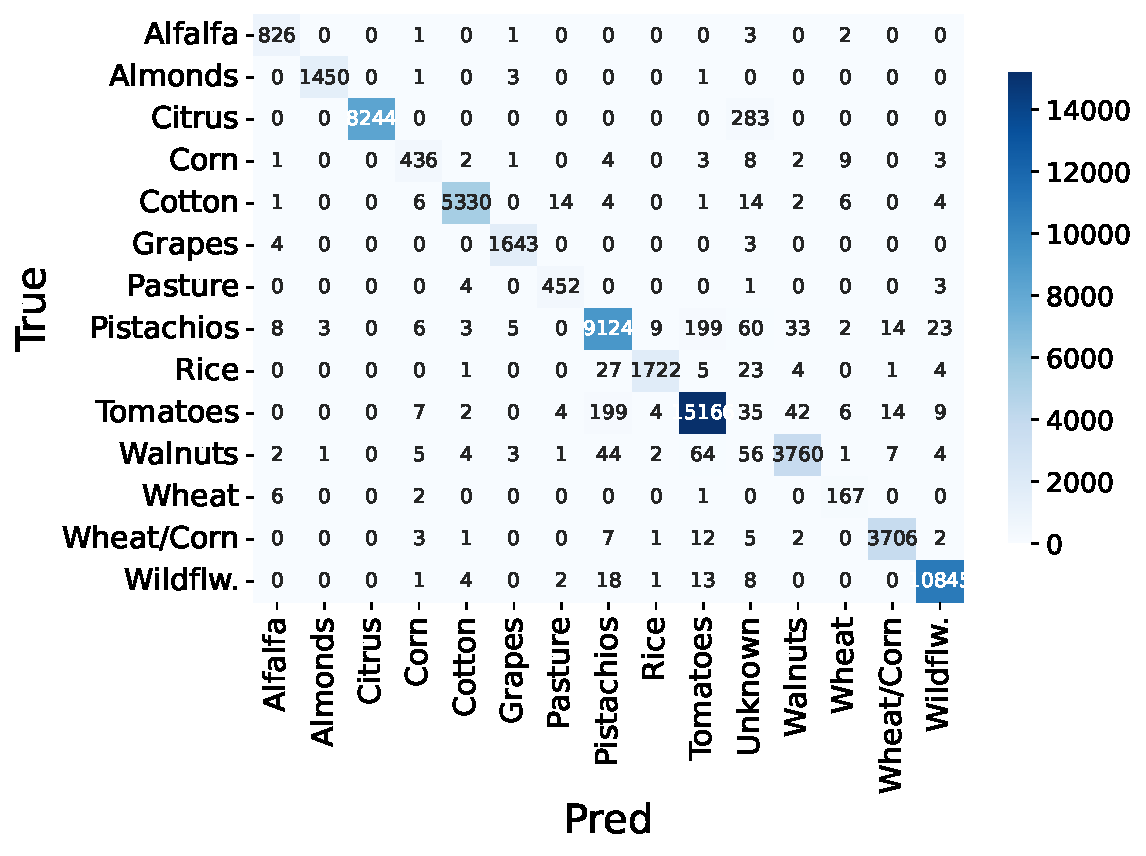
\includegraphics[width=\linewidth]{figures/8_results/california-finetuning/MAMBA-70.0-reconstruct/class_test_gemmos_matrix.pdf}
        %\caption{Matriz de Confusão}
        \label{fig:california_cm}
    \end{subfigure}
    \hfill % Adiciona espaço elástico entre as figuras
    % Início da segunda subfigura (Relatório)
    \begin{subfigure}[b]{0.48\textwidth}
        \centering
        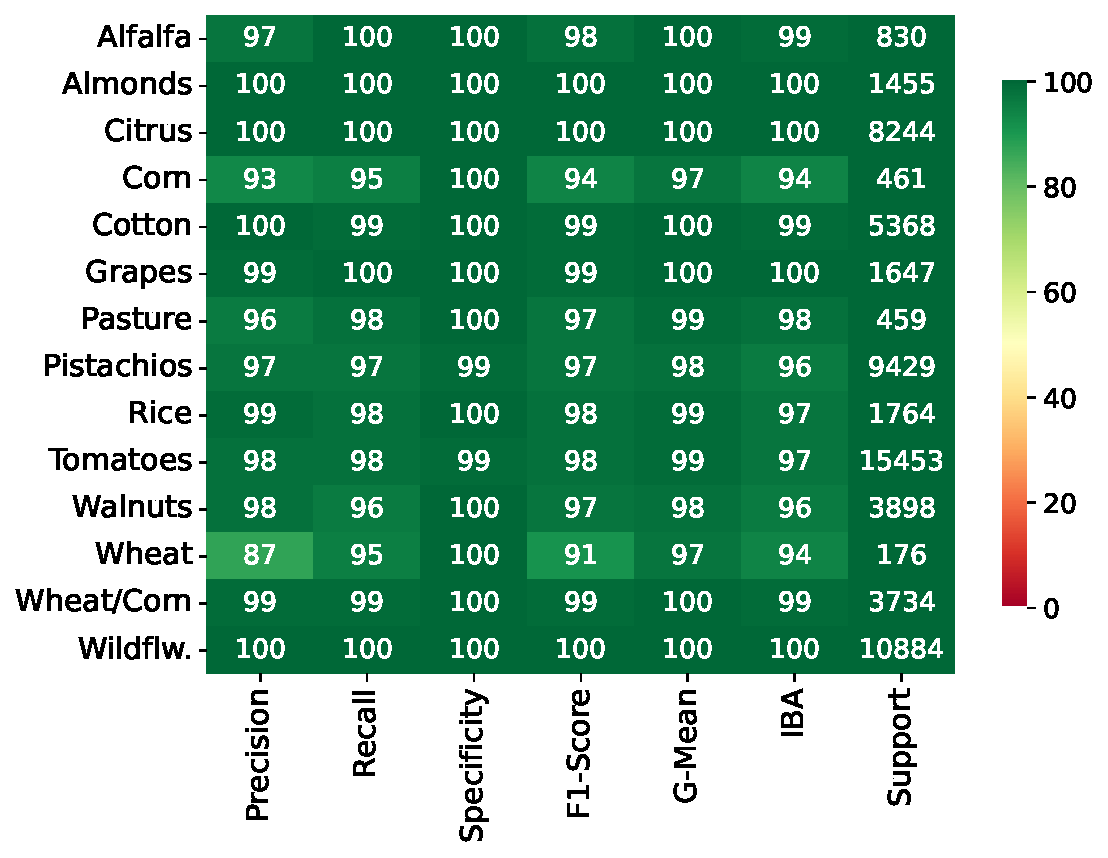
\includegraphics[width=\linewidth]{figures/8_results/california-finetuning/MAMBA-70.0-reconstruct/class_test_gemmos_report.pdf}
        %\caption{Relatório de Classificação}
        \label{fig:california_cr}
    \end{subfigure}
    
    % Legenda geral para ambas as figuras
    \caption{Best experiment in California Dataset with 70\% in training data (Mamba with MM pretraining)..}
    \label{fig:california_experiments}
\end{figure}

Doing the same with the California dataset (see \autoref{fig:california_experiments}), the best experiment on this dataset was using the Mamba model with MM pretraining, demonstrating a robust performance across most agricultural classes. The confusion matrix exhibits a well-defined main diagonal, with near-perfect classification for categories such as Almonds, Citrus, and Wildflow. There is a  consistently high and F1-Score values.

However, the analysis of misclassifications reveals specific spectral-temporal overlaps, most notably between Pistachios and Tomatoes, which accounted for the largest volume of mutual confusion. Additionally, the Wheat class presented the lowest precision (87\%), frequently being mistaken for Alfalfa or Rice, likely due to similarities in phenological cycles or its relatively lower sample support compared to dominant classes.

\begin{figure}[ht!]
    \centering
    \caption{Best experiment in California Dataset with 70\% in training data (Mamba with MM pretraining) separability between right and wrong predictions with ORDER.}
    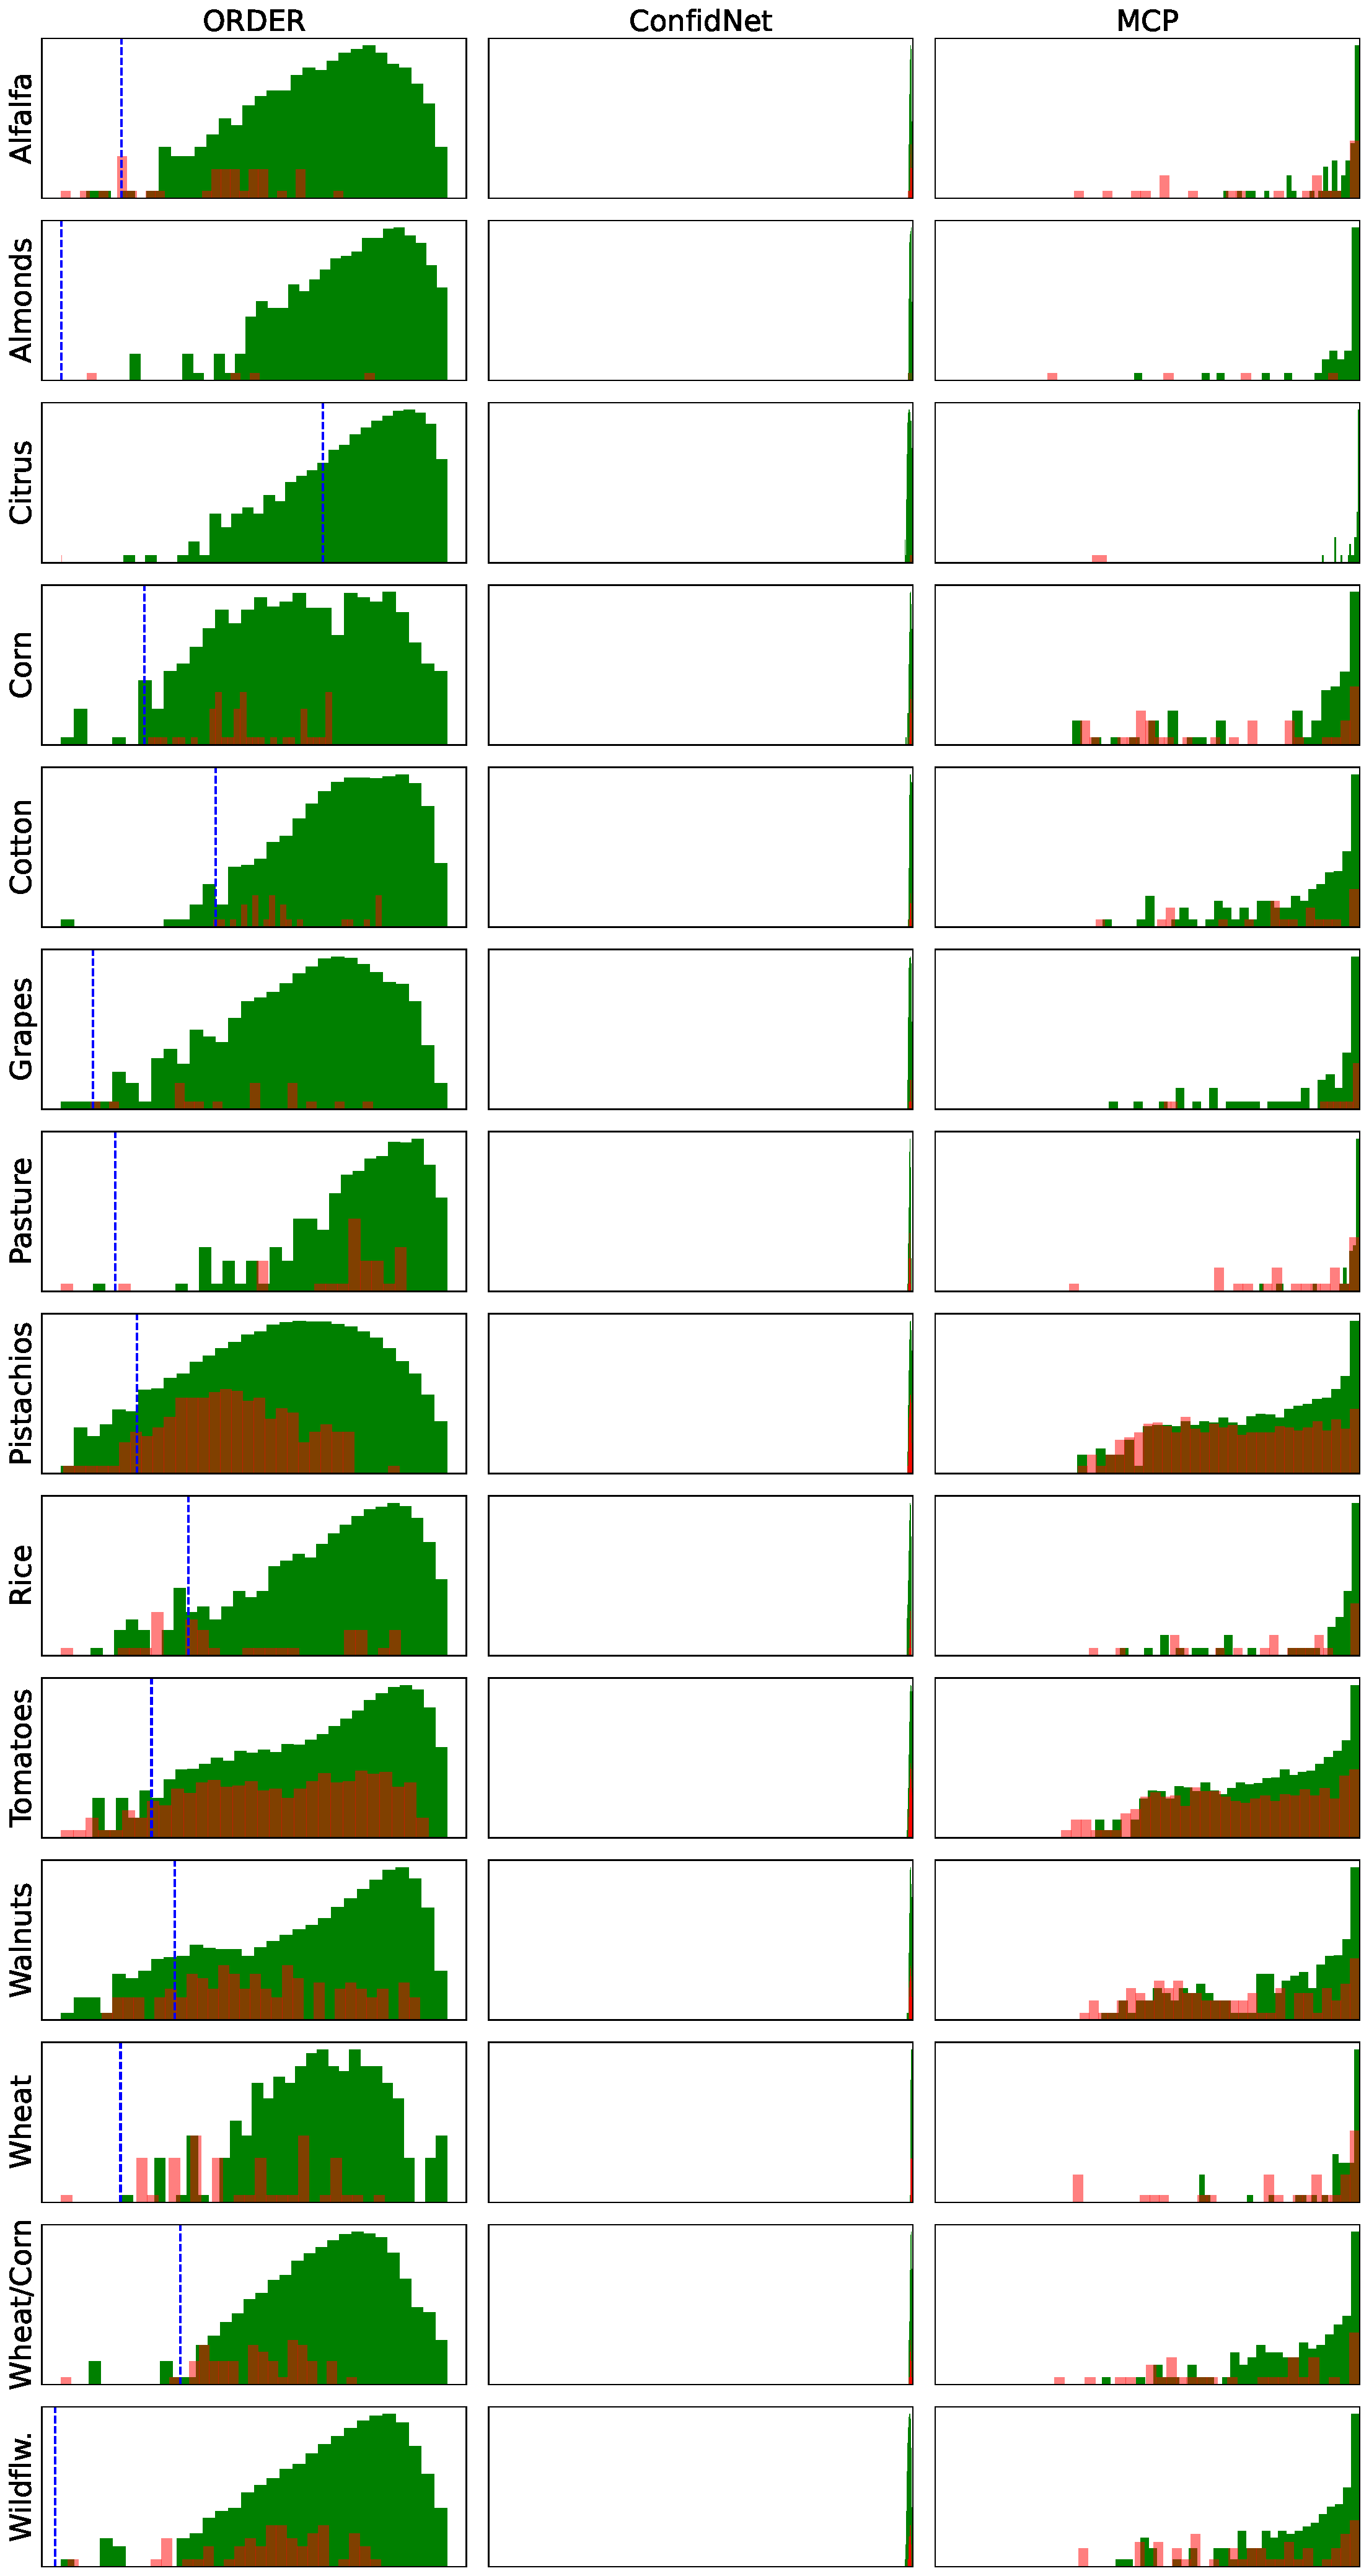
\includegraphics[width=0.6\linewidth]{figures/8_results/california-finetuning/MAMBA-70.0-reconstruct/hist_combined_test.pdf}
    \label{fig:california_gmm}
    \fignote{Y-axis is in logarithmic scale.}
\end{figure}

Again, it is very difficult to determine the effectiveness of ORDER (see \autoref{fig:california_gmm}) given a model with such high evaluation metrics. However, at least the scores are not all saturated close to 1, as is the case with ConfidNet and MCP. Thus, it seems more likely that the strategy would work if there were more challenging samples than the baselines.
\chapter{Conclusion}
\label{chapter:conclusion}

This work presented and validated, through experimental benchmarks, a lightweight pipeline for classifying agricultural crops at the plot level using SITS. As explained, only public labels were used, both from crop mapping and geometry delineation, as well as sensors from public missions. Therefore, this pipeline can be used for low-cost large-scale agricultural monitoring in large countries like Brazil, potentially helping to identify agricultural activities carried out in environmentally protected areas or with unsustainable management practices, and to provide agricultural credit in a fairer and more accurate way.

The experimental results demonstrated that the lightweight download strategy, implemented in our public library AgriGEE.lite, is effective in converting raw data from optical sensors -- such as Sentinel 2 -- into robust statistical representations such as the median-based pseudo-pixels used, enabling large-scale processing without the need for prohibitive hardware infrastructure. Although the library is specifically developed for Google Earth Engine, the methodology can be adapted to other geospatial data processing platforms. Data curation -- also present in the library -- using filters based on vegetation indices and label consistency, allowed the creation of reliable datasets for Brazil, Texas, and California, mitigating noise even in non-agricultural-specific sources such as MapBiomas Brazil.

Regarding model performance, the DL models, specifically SITS-BERT++ and SITS-Mamba, consistently outperformed the SL models, such as RF and SVM, especially in the Brazilian dataset, which presents greater complexity and higher label noise. However, in regional scenarios with less variability, such as Texas and California, simpler and lighter models remained competitive.

Experiments with SSL confirmed that pre-training strategies, particularly Momentum Contrast (MoCo) and Masked Modeling (MM), appear to be impactful in few shot regimes. In the Brazilian dataset, the use of SSL resulted in gains of up to 40\% in F1 Weighted when only 1\% of the labeled data was available for training.

Finally, the proposed \ac{ORDER} method, an evolution of the GeMOS framework but focused on anomaly detection, visually demonstrated greater separation between correct and incorrect predictions when compared to the ConfidNet baseline or the model itself. 

Considering all experiments, in an unknown scenario, it would be wise to opt for the SITS-BERT++ or SITS-Mamba model with MoCo pretraining using \ac{ORDER} for anomaly detection. The choice between the two models will depend on the available computational resources or other data that can be integrated, since SITS-Mamba is much lighter and faster due to its linear complexity, while SITS-BERT++ offers slightly superior performance. Furthermore, it is noteworthy that the SITS-Mamba showed more consistent performance in different pre-training sessions or even when trained from scratch, demonstrating that the model may be more stable and should be chosen when there is limited time/resources for extensive training and results analysis.

Comparing the metrics reported by Mapbiomas and USDA, it is possible to affirm that the pipeline is capable of reconstructing the agricultural classes of these two rasters, demonstrating the viability of its use for large-scale agricultural monitoring. Furthermore, through other rasters from other countries (such as EUCROPMAP\footnote{EUCROPMAP in Google Earth Engine - \url{https://developers.google.com/earth-engine/datasets/catalog/JRC_D5_EUCROPMAP_V1}} or Canada AAFC Annual Crop\footnote{Canada AAFC Annual Crop Inventory in Google Earth Engine - \url{https://developers.google.com/earth-engine/datasets/catalog/AAFC_ACI}}) and the plot design of VARDA itself or the Fields of the World dataset (see \autoref{sec:labeled_datasets}), it is possible to advance in the attempt to create a global crop classification dataset, a kind of Crops of the World. Such a dataset can serve as a more solid benchmark for crop mapping models.

With these conclusions in mind, it is possible to address the research questions raised in Section \ref{chapter:introduction}:

\begin{enumerate}[label=\textbf{RQ\arabic*:}, leftmargin=*, parsep=1em]

    \item \textbf{To what extent can DCAI strategies - specifically, rigorous filtering of noisy public labels (such as USDA CDL or Mapbiomas) - enable the creation of crop classification datasets and improve the performance of crop classification models?}
    
    \begin{itemize}[label=$\hookrightarrow$, leftmargin=2em, topsep=0.5em]
        \item \textbf{Answer:}
        DCAI strategy, combined with public cropland rasters, allows the creation of crop classification datasets. However, to estimate the impacts of DCAI performance, further studies would be necessary, especially to correct possible incorrect labels, analyzing which samples were erroneously predicted and erroneously confirmed by ORDER, as these are possible classification errors.
    \end{itemize}

    \item \textbf{Do SSL pre-training strategies impact embedding generation and offer a significant advantage over supervised models when labels are scarce? If so, which strategy generates the best embeddings?}
    
    \begin{itemize}[label=$\hookrightarrow$, leftmargin=2em, topsep=0.5em]
        \item \textbf{Answer:}
        Using SSL pretraining is a great option for improving classification metrics in scenarios with a shortage of labels, as demonstrated mainly in experiments with 1\% and 0.1\% of labeled data. Regarding strategies, MoCo stands out for generating good metrics in fine-tuning and with KNN trained directly on the embeddings, and it did not present very poor results in any experiment, which shows that it is a very solid choice.
    \end{itemize}

    \item \textbf{Is it possible to build a lightweight pipeline that achieves satisfactory performance for crop classification that can be run without expensive hardware? If so, which models are most suitable?}
    
    \begin{itemize}[label=$\hookrightarrow$, leftmargin=2em, topsep=0.5em]
        \item \textbf{Answer:}
        Yes, such a pipeline seems possible. The SITS download method presented shifts most of the processing cost to the server, allowing the use of cloud solutions like GEE on modest hardware. Regarding the cost of the models, although due to time and research scope constraints their memory size was not explored, all are capable of being fine-tuned on a modest GPU (in some of our tests, we used an Nvidia RTX 5070 TI 16GB). Regarding which model to choose, two stood out: SITS-BERT++ and Mamba. The former presented slightly higher metrics than the latter, which in turn shows linear processing and memory costs instead of the quadratic cost of the former, proving to be a balanced option in terms of cost metrics.
    \end{itemize}

    \item \textbf{Is it possible to achieve satisfactory performance for crop classification using only public sensors?}
    
    \begin{itemize}[label=$\hookrightarrow$, leftmargin=2em, topsep=0.5em]
        \item \textbf{Answer:}
        It appears possible to generate good ranking metrics from public missions. However, further studies with comparative tests against private missions are needed, which can be done using some publicly available datasets.
    \end{itemize}

    \item \textbf{Is it possible to improve confidence estimation or detect model anomalies - differ between right and wrong predictions - through generative models on embeddings, surpassing established baselines such as ConfidNet \citep{corbiere2019addressing} in the task of fault prediction?}
    
    \begin{itemize}[label=$\hookrightarrow$, leftmargin=2em, topsep=0.5em]
        \item \textbf{Answer:}
        It is indeed possible to detect anomalies in the model's prediction time using analysis methods on the embeddings generated during prediction, such as ORDER, generating a visually greater differentiation between correct and incorrect predictions than the ConfidNet baseline or the model itself through MCP. For confidence estimation, the ConfidNet baseline proved to be equal to or even worse visually than the model itself through MCP. It seems possible to create a confidence estimate with ORDER due to the good behavior of the predicted scores, however this was not done and could be done in future work.
    \end{itemize}

\end{enumerate}

Future work could expand the pipeline using more data, whether more spatial statistics for each plot – beyond the median – or the incorporation of data from other sensors such as radars (for example, Sentinel 1 or PalSAR). Another possibility is the incorporation of auxiliary data, such as climate or soil information, from public models/sources. Furthermore, sacrificing some scalability, it would be interesting to explore DL architectures that incorporate spatial information, transforming the classification pipeline into semantic segmentation of SITS images, including the possibility of creating embedding rasters, which can act as data compression for downstream models of other agricultural tasks. To address current limitations, future studies should also explore the use of the \ac{ORDER} framework to proactively clean datasets prior to transfer learning, such as when adapting models trained on Texas data to California environments. Finally, transforming the \ac{ORDER} anomaly outputs into a calibrated confidence score—utilizing techniques like quantile mapping or linear regression—represents a highly valuable next step to better quantify predictive uncertainty and increase the operational reliability of the pipeline.

\postextual

\bibliography{references}

\end{document}